%%%%%%%%%%%%%%%%%%%%%%%%%%%%%%%%%%%%%%%%%%%%%%%%%%%%%%%%%%%%%%%%%%%%%%%%%%%%%%%
%%%%%%%%%%%%%%%%%%%       ADVANCED PROGRAMMING         %%%%%%%%%%%%%%%%%%%%%%%
%%%%%%%%%%%%%%%%%%%%%%%%%%%%%%%%%%%%%%%%%%%%%%%%%%%%%%%%%%%%%%%%%%%%%%%%%%%%%%%
% !TeX program = lualatex
\documentclass[a4paper,10pt,twoside,english]{book}
%\documentclass[a4paper,twoside,english]{book}


\usepackage[
paperwidth=16.99cm,
paperheight=24.40cm,
left=2.4cm,
right=2cm,
top=2.95cm,
bottom=2.2cm,
twoside
]{geometry}


\usepackage[width=16.99truecm,height=24.40truecm,center]{crop}
%\usepackage[frame,width=16.99truecm,height=24.40truecm,center]{crop}
%\usepackage[a4,frame,center]{crop}


\usepackage{epic}
% Paquetes adicionales
\usepackage[utf8]{inputenc} % Codificación de caracteres
\usepackage[spanish]{babel} % Soporte para español
\usepackage{amsmath} % Paquete para matemáticas


% Paquetes para gráficos
\usepackage{graphicx}
\usepackage{tikz}
\usepackage{pgfplots}
\pgfplotsset{compat=1.17}


\usepackage{fancyhdr}
\usepackage[a4paper, margin=1in]{geometry}
\usepackage{afterpage}
\usepackage{titlesec} % O sectsty para modificar títulos y secciones.



\usepackage{hyperref} % Paquete para enlaces y referencias
\usepackage{xcolor}
\usepackage{tcolorbox}
\usepackage{verbatim}



\usepackage{listings}
\usepackage{listingsutf8}

\lstdefinelanguage{Julia}{
  morekeywords={
    abstract, break, case, catch, const, continue, do, else, elseif, end, export, false, for, function, immutable, import, in, macro, module, true, try, using, while, struct, mutable, return
  },
  sensitive=true,
  morecomment=[l]\#,
  morestring=[b]",
  morestring=[b]',
}

\lstset{
  language=Julia,
  backgroundcolor=\color{gray!0},
  basicstyle=\ttfamily\footnotesize,
  keywordstyle=\color{blue},
  commentstyle=\color{black!30},
  stringstyle=\color{red},
  numbers=left,
  numberstyle=\tiny,
  stepnumber=1,
  numbersep=10pt,
  showstringspaces=false,
  tabsize=4,
  breaklines=true,
  breakatwhitespace=false,
  frame=single,
  columns=fullflexible
}

% ________________________CODE LENGUAGE________________________________________
\usepackage{listings}

\lstdefinelanguage{JavaScript}{
	keywords={typeof, new, true, false, catch, function, return, null, catch, switch, var, if, in, while, do, else, case, break, undefined},
	keywordstyle=\color{blue}\bfseries,
	ndkeywords={class, export, boolean, throw, implements, import, this},
	ndkeywordstyle=\color{darkgray}\bfseries,
	identifierstyle=\color{black},
	sensitive=false,
	comment=[l]{//},
	morecomment=[s]{/*}{*/},
	commentstyle=\color{red}\ttfamily,
	stringstyle=\color{orange}\ttfamily,
	morestring=[b]',
	morestring=[b]"
}



%\lstset{literate=%
%	{0}{{{\color{Green}0}}}1
%	{1}{{{\color{Green}1}}}1
%	{2}{{{\color{Green}2}}}1
%	{3}{{{\color{Green}3}}}1
%	{4}{{{\color{Green}4}}}1
%	{5}{{{\color{Green}5}}}1
%	{6}{{{\color{Green}6}}}1
%	{7}{{{\color{Green}7}}}1
%	{8}{{{\color{Green}8}}}1
%	{9}{{{\color{Green}9}}}1
%}


\newcommand{\lsthtml}{
	\lstset{
		language=html,
		basicstyle=\ttfamily\small,
		frame=single,
		showspaces=false,
		showstringspaces=false,
		backgroundcolor=\color{white},
		keywordstyle=\color{blue},
		deletekeywords={type},
		commentstyle=\color{mygreen},
		stringstyle=\color{violet},
		breaklines=true,
		alsoletter={.},morekeywords={nav,/nav}
	}
}
\newcommand{\lstbash}{
	\lstset{
		language=bash,
		basicstyle=\ttfamily\small,
		frame=single,
		showspaces=false,
		showstringspaces=false,
		backgroundcolor=\color{white},
		keywordstyle=\color{blue},
		deletekeywords={type},
		commentstyle=\color{mygreen},
		stringstyle=\color{violet},
		breaklines=true,
		alsoletter={.},
		morekeywords={ssh,scp,server.py,runserver.sh,killserver.sh,killemail.sh,runemail.sh}
	}
}


%\newcommand{\lstpython}{
%	\lstset{
%		language=python,
%		basicstyle=\footnotesize\ttfamily,
%		frame=single,
%		showspaces=false,
%		showstringspaces=false,
%		backgroundcolor=\color{gray!2},
%		keywordstyle=\normalsize\bfseries,
%		deletekeywords={type},
%        commentstyle=\color{gray!50},
%        captionpos=b, % sets the caption-position to bottom
%		stringstyle=\color{gray},     % string literal style
%		breaklines=true,
%        breakatwhitespace=false, 
%		alsoletter={.,...},
%		morekeywords={},
%        tabsize=2, % sets default tabsize to 2 spaces
%        numberstyle=\tiny, % the size of the fonts that are used for the line-numbers     
%        numberstyle = \color{black},
%        rulesepcolor=\color{gray},
%        frame=trBL,
%        showtabs=false % show tabs within strings adding particular underscores
%	}
%}





\newcommand{\lstjs}{
	\lstset{
		language=JavaScript,
		extendedchars=true,
		basicstyle=\ttfamily\footnotesize,
		frame=single,
		showstringspaces=false,
		showspaces=false,
		numberstyle=\footnotesize,
		numbersep=9pt,
		tabsize=4,
		breaklines=true,
		showtabs=false,
		captionpos=b
	}
}




%
%
%\lstset{ %
%	backgroundcolor=\color{white},   % choose the background color; you must add \usepackage{color} or \usepackage{xcolor}
%	basicstyle=\footnotesize,%%        % the size of the fonts that are used for the code
%	breakatwhitespace=false,         % sets if automatic breaks should only happen at whitespace
%	breaklines=true,                 % sets automatic line breaking
%	captionpos=b,                    % sets the caption-position to bottom
%	commentstyle=\color{mygreen},    % comment style
%	deletekeywords={...},            % if you want to delete keywords from the given language
%	escapeinside={\%*}{*)},          % if you want to add LaTeX within your code
%	extendedchars=true,              % lets you use non-ASCII characters; for 8-bits encodings only, does not work with UTF-8
%	frame=single,                    % adds a frame around the code
%	keepspaces=true,                 % keeps spaces in text, useful for keeping indentation of code (possibly needs columns=flexible)
%	keywordstyle=\color{blue}\textbf,       % keyword style
%	language=Fortran,                 % the language of the code
%	otherkeywords={*,source},            % if you want to add more keywords to the
%	% set
%	numbers=none,                    % where to put the line-numbers; possible
%	% values are (none, left, right)
%	numbersep=5pt,                   % how far the line-numbers are from the code
%	numberstyle=\tiny\color{mygray}, % the style that is used for the line-numbers
%	rulecolor=\color{black},         % if not set, the frame-color may be changed on line-breaks within not-black text (e.g. comments (green here))
%	showspaces=false,                % show spaces everywhere adding particular underscores; it overrides 'showstringspaces'
%	showstringspaces=false,          % underline spaces within strings only
%	showtabs=false,                  % show tabs within strings adding particular underscores
%	stepnumber=2,                    % the step between two line-numbers. If it's 1, each line will be numbered
%	stringstyle=\color{mymauve},     % string literal style
%	tabsize=2,                       % sets default tabsize to 2 spaces
%	title=\lstname                   % show the filename of files included with \lstinputlisting; also try caption instead of title
%}
%
%
%


%\lstset{ %
%	backgroundcolor=\color{Goldenrod!10},   % choose the background color; you must add \usepackage{color} or \usepackage{xcolor}
%	basicstyle=\footnotesize\ttfamily,%%\small,               % the size of the fonts that are used for the code
%	breakatwhitespace=false,                % sets if automatic breaks should only happen at whitespace
%	breaklines=true,                 % sets automatic line breaking
%	captionpos=b,                    % sets the caption-position to bottom
%	commentstyle=\color{mygreen},    % comment style
%	deletekeywords={...},            % if you want to delete keywords from the given language
%	escapeinside={\%*}{*)},          % if you want to add LaTeX within your code
%	extendedchars=true,              % lets you use non-ASCII characters; for 8-bits encodings only, does not work with UTF-8
%	frame=single,                    % adds a frame around the code
%	keepspaces=true,                 % keeps spaces in text, useful for keeping indentation of code (possibly needs columns=flexible)
%	keywordstyle=\color{blue}\textbf,       % keyword style
%	language=Fortran,                 % the language of the code
%	otherkeywords={*,source},            % if you want to add more keywords to the
%	% set
%	numbers=none,                    % where to put the line-numbers; possible
%	% values are (none, left, right)
%	numbersep=5pt,                   % how far the line-numbers are from the code
%	numberstyle=\tiny\color{mygray}, % the style that is used for the line-numbers
%	rulecolor=\color{black},         % if not set, the frame-color may be changed on line-breaks within not-black text (e.g. comments (green here))
%	showspaces=false,                % show spaces everywhere adding particular underscores; it overrides 'showstringspaces'
%	showstringspaces=false,          % underline spaces within strings only
%	showtabs=false,                  % show tabs within strings adding particular underscores
%	stepnumber=2,                    % the step between two line-numbers. If it's 1, each line will be numbered
%	stringstyle=\color{mymauve},     % string literal style
%	tabsize=2,                       % sets default tabsize to 2 spaces
%%	title=\texttt{\detokenize{\lstname}}     % show the filename of files included with \lstinputlisting; also try caption instead of title
%%	title= \texttt{\lstname}
%%    caption =\texttt{\detokenize{\lstname}}
%%    caption =\detokenize{\lstname}
%}




%\newcommand{\lstfor}{
% \lstset{ 
%    language=Fortran, % choose the language of the code
%    % basicstyle=\footnotesize\ttfamily,
%    % keywordstyle=\color{black}\textit, % style for keywords
%    basicstyle=\footnotesize\ttfamily,
%    keywordstyle=\normalsize\bfseries,%\textit, %%
%    numbers=none, % where to put the line-numbers
%    numberstyle=\tiny, % the size of the fonts that are used for the line-numbers     
%    backgroundcolor=\color{gray!2},
%    showspaces=false, % show spaces adding particular underscores
%    showstringspaces=false, % underline spaces within strings
%    showtabs=false, % show tabs within strings adding particular underscores
%    frame=single, % adds a frame around the code
%    tabsize=2, % sets default tabsize to 2 spaces
%    rulesepcolor=\color{gray},
%    stringstyle=\color{gray},     % string literal style
%    captionpos=b, % sets the caption-position to bottom
%    breaklines=true, % sets automatic line breaking
%    breakatwhitespace=false, 
%    commentstyle=\color{gray!50},
%    numberstyle = \color{black},
%    frame=trBL,
%    morekeywords={procedure, findloc}
%}
%}


\newcommand\mycap[1]{ \texttt{ \detokenize{#1} }  }


\definecolor{mymauve}{rgb}{0.58,0,0.82}


\definecolor{codegreen}{rgb}{0,0.6,0}
\definecolor{codegray}{rgb}{0.5,0.5,0.5}
\definecolor{codepurple}{rgb}{0.58,0,0.82}
\definecolor{backcolour}{rgb}{0.95,0.95,0.92}

\newcommand{\lstfor}{
 \lstset{ 
     language=Fortran, % choose the language of the code
      morekeywords=[1]{,imag,procedure,abstract,findloc},
    % basicstyle=\footnotesize\ttfamily,
   %  keywordstyle=\color{black}\textit, % style for keywords
     basicstyle=\footnotesize\ttfamily,
     keywordstyle=\color{blue}\normalsize\bfseries,%\textit, %%
     numbers=none, % where to put the line-numbers
     numberstyle=\tiny, % the size of the fonts that are used for the line-numbers     
     backgroundcolor=\color{blue!1},
  %   backgroundcolor=\color{blue!5!white},
     showspaces=false, % show spaces adding particular underscores
     showstringspaces=false, % underline spaces within strings
     showtabs=false, % show tabs within strings adding particular underscores
     frame=single, % adds a frame around the code
  %   rulecolor=\color{black},
     rulecolor=\color{Blue!75!black},
     tabsize=2, % sets default tabsize to 2 spaces
  %   rulesepcolor=\color{blue},
     rulesepcolor=\color{Blue!75!black},
     stringstyle=\color{orange},     % string literal style
     captionpos=b, % sets the caption-position to bottom
     breaklines=true, % sets automatic line breaking
     breakatwhitespace=false, 
     commentstyle=\color{codegreen},
     numberstyle = \color{black},
     frame=trBL,
     %morekeywords={class,imag,procedure, abstract, findloc}
  %    morekeywords=[1]{,imag,procedure,abstract,findloc}
 }
}



\newcommand{\lstpython}{
 \lstset{ 
     language=Python, % choose the language of the code
     commentstyle=\color{codegreen}\ttfamily,
    % basicstyle=\footnotesize\ttfamily,
   %  keywordstyle=\color{black}\textit, % style for keywords
     basicstyle=\footnotesize\ttfamily,
     keywordstyle=\color{blue}\normalsize\bfseries,%\textit, %%
     numbers=none, % where to put the line-numbers
     numberstyle=\tiny, % the size of the fonts that are used for the line-numbers     
     backgroundcolor=\color{blue!1},
     showspaces=false, % show spaces adding particular underscores
     showstringspaces=false, % underline spaces within strings
     showtabs=false, % show tabs within strings adding particular underscores
     frame=single, % adds a frame around the code
   %  rulecolor=\color{black},
     rulecolor=\color{Blue!75!black},
     tabsize=2, % sets default tabsize to 2 spaces
   %  rulesepcolor=\color{blue},
     rulesepcolor=\color{Blue!75!black},
     stringstyle=\color{orange},     % string literal style
     captionpos=b, % sets the caption-position to bottom
     breaklines=true, % sets automatic line breaking
     breakatwhitespace=false, 
     numberstyle = \color{black},
     frame=trBL,
     morekeywords={}
 }
}

%%%% LUA MACRO FOR EXTRACTING A PIECE 

\directlua{

function create_file(file, label1, label2)

    local write =  false; 
    local temp = io.open("temp.f90", "w"); 

    for line in io.lines(file) do 

          if string.match( line, label1) then
                                              write = true; 
          end

          if write then 

             if string.match( line, label2) then
                    write = false; 
                    temp:write(line, "\string\n"); 
                    temp:close(); 
                    return; 
             else 
                    temp:write(line, "\string\n"); 
             end 
                  
          end
     end  

end
} 


\newcommand{\ExtractCode}[3]{
	\directlua
	{ 
		create_file(#1, #2, #3)
	}
}%


\newcommand{\listings}[4]{
	\ExtractCode{"#1"}{"#2"}{"#3"}
	\lstinputlisting[language=Fortran, firstline = 1, lastline = 500, caption = \mycap{#4}]{temp.f90}	
}
\newcommand{\listingsp}[4]{
	\ExtractCode{"#1"}{"#2"}{"#3"}
	\lstinputlisting[language=Python, firstline = 1, lastline = 500, caption = \mycap{#4}]{temp.f90}	
}





%\usepackage{parskip}
%\setlength{\parskip}{1cm plus 4mm minus 3mm}
%\setlength\parindent{18pt}



\graphicspath{ {images/} }
\newcommand{\folder}{./libraries}

\usepackage{amsfonts}

%MIGUEL
\usepackage{rotating}
\newcommand\myfunc[5]{%
    \begingroup
    \setlength\arraycolsep{0pt}
    #1\colon\begin{array}[t]{c >{{}}c<{{}} c}
        #2 & \to & #3 \\ #4 & \to & #5 
    \end{array}%
    \endgroup}


\usepackage{amsmath}
%\DeclareMathOperator{\Tr}{Tr}



%LINEAS NUEVAS
\newlength\myheight
\newlength\mydepth
\settototalheight\myheight{Xygp}
\settodepth\mydepth{Xygp}
\setlength\fboxsep{0pt}


% Replace the title of the table of contents 
\addto\captionsenglish{
    \renewcommand{\contentsname}%
    {Contents}% Here it goes the new title
}


%_______________________________________________________________________________
\usepackage{titling} % Allows custom title configuration

\bibliographystyle{abbrvnat}
\addto\captionsenglish{\renewcommand{\bibname}{References}}		%It changes name of bibliography to References using natbib

\definecolor{DarkGoldenrod}{rgb}{0.8,0.6,0.1}
\definecolor{DarkRed}{rgb}{0.5,0.1,0.1}
\definecolor{DarkRedPart}{rgb}{0.3,0.1,0.2}

% Defines the gold horizontal rule around the title
%\newcommand{\HorRule}{\color{DarkGoldenrod} \rule{\linewidth}{1pt}}

%Makes the font of the bibliography a little bit smaller to adjust it to one page.
\renewcommand*{\bibfont}{\footnotesize} 


% Horizontal rule before the title
\pretitle{\vspace{-150pt} \begin{flushleft} \HorRule \fontsize{34}{34}
		\usefont{OT1}{phv}{b}{n} \color{DarkRed} \selectfont}
	% Your article title	
	\title{{\fontsize{27}{33}\selectfont Advanced Programming for \\ Numerical Calculations: 
	 \\  \vspace{0.8cm} } 
	 {\fontsize{27}{33}\selectfont Climbing Python \& Fortran\\ }
	 }
	
	% Whitespace under the title	
	\posttitle{\par\end{flushleft}\vskip 0.5em} 

% Author font configuration
\preauthor{	
\begin{flushleft} 
    \large \lineskip 0.5em \usefont{OT1}{phv}{b}{sl} \color{DarkRed}}	 	
	\author{ Juan Antonio Hern\'andez Ramos\\ 	
  	         Miguel \'Angel Rapado Tamarit\\
            \vspace{5cm} } % Your name. En función de los nombres poner más espacio en el vspace o menos, para dejar la línea abajo del todo
         
        % Configuration for the institution name
        \postauthor{\footnotesize \usefont{OT1}{phv}{m}{sl} \color{Black}
        Department of Applied Mathematics \\
        School of Aeronautical and Space Engineering \\
        Technical University of Madrid (UPM)		
	\par 
\end{flushleft}
\HorRule % Horizontal rule after the title
}

\date{  } % Add a date here if you would like one to appear underneath the title block


\usepackage{tocloft}
\setlength{\cftbeforechapskip}{0.4cm}

\usepackage{hyperref}

\newcommand{\link}[2]
{  
\color{red}    
\href{#2}{#1}                     
\color{black}  
}

%%%%%%%%%%%%%%%%%%%%%%%%%%%%%%%%%%%%%%%%%%%%%%%%%%%%%%%%%%%%%%%%%%%%%%%%%%%%%%%%%%%%%%%%%%%%%%%%%%%%%%%%%%
%%%%%%%%%%%%%%%%%%%%%%%%%%%%%%%%%%%%%%%%%%%%%%%%%%%%%%%%%%%%%%%%%%%%%%%%%%%%%%%%%%%%%%%%%%%%%%%%%%%%%%%%%%
%\pagestyle{empty}
\begin{document}
 
  
   
    \maketitle
    \thispagestyle{empty}   %Le quita el número de página y las líneas arriba y abajo a la parte de atrás de la portada. 
    %\cleardoublepage       %Deja en blanco la página de detrás de la portada y no se numera
    
    %______________________________________________________________________________________________________
    %Para la página de detrás de la portada, la hacemos a mano que es más sencillo y da menos problemas.  
    
    \noindent  Cover: 
    \vspace{0.2cm}
    
    \noindent Programming and mountain climbing are not such dissimilar activities. 
    In both worlds, you start slowly, little by little. 
    We start programming with a ``hello world" just as we start 
    with a circular route of a few kilometers and little slope.
     But as time goes by, we add time spent in routes with family and friends 
     and scripts to solve class work, personal projects, or even complete doctoral theses.
    
    This book is the last slope before reaching the peak. 
    It's that urge to say: ``come on, there's nothing left, there's the summit" after several kilometers. 
    In this book, you will find advanced programming techniques of two great languages, 
    Python and Fortran, to climb the ``numerical calculations" like a true professional.
    
    These words are inspired by the photo on the cover of this book. The photo was taken in the last minutes of arriving at the Urriellu 
    refuge in Asturias, Spain.
    
    I hope you enjoy this book as much as I enjoy programming and climbing mountains. 
    Thank you, dad, for showing me both worlds.
    
    \vspace{1cm}
    \noindent Cover design: 
    \vspace{0.2cm}
    
    \noindent Laura Hernández \& Cristina de Lorenzo
   
 
    \vfill  
    \begin{minipage}[b]{0.9\textwidth}
     %   This manual is aimed at the Aerospace Engineering students of the Technical University of Madrid who may start programming different 
     %languages with Microsoft Visual Studio. It is also for anyone interested in start using this complete tool from scratch. Additional 
     %content can be downloaded from \url{https://github.com/jahrWork}. The manual has been written with the idea of increasing all the 
     %information presented and improving the contents. Ideas for something to be added, deleted or changed would be kindly appreciated. In 
     %addition, corrections and feedback about anything that could be improved or better explained are welcomed. All contributions can be 
     %made 
     %in:
        
%        \vspace*{2\baselineskip}
%        Miguel Ángel Rapado Tamarit \newline
%        \textcolor{Blue}{marapadotamarit@gmail.com}
%        \vspace*{3\baselineskip}
%        
        %\footnotesize\raggedright
        
    \end{minipage}
    
    \noindent
    All rights reserved.
    No part of this publication may be reproduced or transmitted in any form or by any means, electronic or mechanical, including photocopy, recording, or any information storage and retrieval system, without permission in writing from the authors. 
    \vspace{2\baselineskip}
    

       \noindent \copyright  \ \ 2022 Juan Antonio Hernández Ramos 
       \hspace{0.7cm}     Miguel Ángel Rapado Tamarit
    
    \vspace{0.5cm}            
    \noindent ISBN 979-8352363232
    %\noindent Depósito Legal: M-3036-2001
    \clearpage
    
  
    %______________________________________________________________________________________________________
    \frontmatter
    
    \pagenumbering{roman}
    
    \parskip = \baselineskip %  plus 4mm minus 3mm}  
   % \input{./doc/Chapters/Preface.tex}
    
    \newpage
    \setlength{\parskip}{0pt}
    \tableofcontents
    ~\clearpage


    \pagenumbering{arabic}
    
    \parskip = \baselineskip
    
    %______________________________________________________________________________________________________
    \mainmatter
  
    \newcommand\home{./Fortran_project/sources/IEEE}
  
   \chapter*{Advanced Programming for Numerical Calculations: Climbing Python \& Fortran}
%addcontentsline{toc}{chapter}{Introduction}
%\thispagestyle{empty}
\vspace{-2.5cm}
This book is devoted to those who like math and  use  
programming languages such as: Python or Fortran to solve numerical problems.  
The main focus of this book is to approach math language to programming languages by 
paying attention to functional programming paradigm.
Through different numerical examples, 
the book tries to mimic mathematics by showing how  mathematical concepts 
are implemented by means of functional programming paradigm. 
 

This book is divided in three parts: 
\begin{itemize}
\setlength\itemsep{0cm}
\item[] Part I. Foundations. 
\item[] Part II. Computer operations with integers and reals. 
\item[] Part III. Advanced programming. 
\end{itemize}
\vspace{-0.2cm}
These three parts can be read  independently. The first part: Foundations is devoted to 
initiate the reader in implementing  numerical problems with the computer.
The second part: Computer operations with integers and reals. 
Real or integer numbers are represented with finite storage. When oerating those numbers, 
errors associated to the loss of precision is encountered. This second part tries to get a deep 
knowledge, by following different examples, of this round-off errors.   
The third part: Advanced programming gives tries to show the most important techniques 
focalizing  mainly in the functional programming paradigm with pure functions 
emulating math environments. 


This book can not be considered a full handbook of Python or Fortran. 
It is a modest approach of challenging numerical problems by means of
functional programming in Python and Fortran. 
This book is fully supported with the following software repository: 
\vspace{-0.2cm}
\begin{center} 
\link{Software repository: jahrWork}{https://github.com/jahrWork/Advanced_programming}
\end{center} 

\newpage 
\subsection*{Fortran menu}
The repository comprises a Fortran project and Python project
implemented in Visual Studio. However, examples can be run with any other different editor or 
Integrated
Development Environment (IDE). 
Once this repository  is downloaded or cloned, the following Fortran main program 
covers different examples for the three parts of this book:   
\vspace{0.5cm}
\lstfor
\renewcommand{\home}{./Fortran/sources} 
\listings{\home/main.f90}{Program main}{end program}{main.f90}

\newpage 
\subsection*{Python menu}
The following Python main program 
covers different examples for the three parts of this book:   
\vspace{0.5cm}
\lstpython
\renewcommand{\home}{./Python/sources} 
\listingsp{\home/main.py}{from}{option not implemented}{main.py}









    
  \part{Foundations}\label{PartI}
         \chapter*{Advanced Programming for Numerical Calculations: Climbing Python \& Fortran}
%addcontentsline{toc}{chapter}{Introduction}
%\thispagestyle{empty}
\vspace{-2.5cm}
This book is devoted to those who like math and  use  
programming languages such as: Python or Fortran to solve numerical problems.  
The main focus of this book is to approach math language to programming languages by 
paying attention to functional programming paradigm.
Through different numerical examples, 
the book tries to mimic mathematics by showing how  mathematical concepts 
are implemented by means of functional programming paradigm. 
 

This book is divided in three parts: 
\begin{itemize}
\setlength\itemsep{0cm}
\item[] Part I. Foundations. 
\item[] Part II. Computer operations with integers and reals. 
\item[] Part III. Advanced programming. 
\end{itemize}
\vspace{-0.2cm}
These three parts can be read  independently. The first part: Foundations is devoted to 
initiate the reader in implementing  numerical problems with the computer.
The second part: Computer operations with integers and reals. 
Real or integer numbers are represented with finite storage. When oerating those numbers, 
errors associated to the loss of precision is encountered. This second part tries to get a deep 
knowledge, by following different examples, of this round-off errors.   
The third part: Advanced programming gives tries to show the most important techniques 
focalizing  mainly in the functional programming paradigm with pure functions 
emulating math environments. 


This book can not be considered a full handbook of Python or Fortran. 
It is a modest approach of challenging numerical problems by means of
functional programming in Python and Fortran. 
This book is fully supported with the following software repository: 
\vspace{-0.2cm}
\begin{center} 
\link{Software repository: jahrWork}{https://github.com/jahrWork/Advanced_programming}
\end{center} 

\newpage 
\subsection*{Fortran menu}
The repository comprises a Fortran project and Python project
implemented in Visual Studio. However, examples can be run with any other different editor or 
Integrated
Development Environment (IDE). 
Once this repository  is downloaded or cloned, the following Fortran main program 
covers different examples for the three parts of this book:   
\vspace{0.5cm}
\lstfor
\renewcommand{\home}{./Fortran/sources} 
\listings{\home/main.f90}{Program main}{end program}{main.f90}

\newpage 
\subsection*{Python menu}
The following Python main program 
covers different examples for the three parts of this book:   
\vspace{0.5cm}
\lstpython
\renewcommand{\home}{./Python/sources} 
\listingsp{\home/main.py}{from}{option not implemented}{main.py}









         \chapter{Basic operations} \label{chap:basicop}

    %\vspace{-1cm}
    \section{Introduction} 
    %\vspace{-0.7cm}
This chapter introduces some of the most basic ingredients of computer programming 
using its foundational concepts of mathematics.
Data types, operators, data structures, etc.
find their origins in mathematical objects.
In a given branch of mathematics, an object is anything that can be formally defined and 
which is subject of deductive reasoning. 
For example, the numbers are objects in the Numbers Theory and
all algebraic structures are objects in Abstract Algebra.
But first let's give some context. 

\textbf{Scientific computing} is considered the third pillar of science. 
Together with a theoretical approach and an experimental approach, 
the complex problems of science and engineering can also be solved 
by means of computers. 
To do that, a computer program is coded following a particular life cycle (see figure \ref{fig:LifeCycle}).
First of all the phenomena of interest must be revised and the \textbf{specifications of the project} defined. 
Then, a \textbf{mathematical model} is built by setting the governing and constitutive equations, the assumptions and constraints of the model, initial and boundary conditions, etc.
With all the tools encompassed in the field of Numerical Analysis, the methods needed to solve the mathematical model are developed, leading to the algorithms. 

An \textbf{algorithm} in mathematics is a finite and ordered sequence of unambiguous instructions to solve a specific problem. 
Notice that this definition involves that i) the algorithm ends in a finite number of steps, 
ii) the sequence of instructions that yields the output are followed in their numerical order and
iii) inputs, instructions and outputs must be properly identified. 

The \textbf{problem} to solve can be seen as a function between a bunch of inputs and their associated outputs.
The algorithm solves an instance of this function, which means, its particularization on a specific set of inputs.
Given a problem, an algorithm to solve it and a machine, 
the theory of computation gives the basis for the automatic processing of the algorithm
and answers things like how efficiently the problem is solved. 

To use machines we need to speak their language, however, machine languages are extremely tough to comprehend by humans.
These languages are known as low-level programming languages and are made of binary numbers carrying processor instructions. 
As an intermediate step, humans use high-level programming languages.
The \textbf{programming code} is the translation or implementation of the algorithm (mathematical language) 
to a language partially understood by the machine, the programming language. 
Notice that an algorithm breaks down a complex problem into simpler instructions 
and then it is translated into a program. 

This program is then compiled or interpreted by a computer program called compiler. 
It is in charge of the final translation from the human-friendly programming language 
into the machine language. As a result, an \textbf{executable code} is generated.
The execution of this code in the machine performs the simulation until the \textbf{numerical results} are obtained.
Here a \textbf{validation} process begins where the output is compared with observations, theoretical models, experiments, etc. 
and the different steps of the cycle are called into question.



 
\usetikzlibrary{shapes.geometric, arrows}

\usetikzlibrary{positioning} 

\tikzstyle{block} = [draw, rectangle, rounded corners, draw=black, very thick,
fill={rgb:orange,1;yellow,2;pink,5},
text width=4cm, text centered, minimum height=1.2cm, node distance=3cm]
\tikzstyle{container} = [draw, rectangle, inner sep=0.3cm]

\tikzstyle{text} = [draw, color=blue]
\tikzstyle{arrow} = [thick,->, >=latex]
\tikzstyle{line} = [thick,-]
 
\begin{figure}[]
\centering

    \begin{tikzpicture}
        
        \node [block, name=s] {Specification};
        \node [block, below of=s] (m) {Math model} ;
        \node [block, below of=m] (a) {Algorithm};
        \node [block, below of=a] (p) {Programming code};
        \node [block, below of=p] (e) {Executable code};
        \node [block, below of=e] (r) {Numerical result};
        
        \node [coordinate, below of=r] (d1) {};
        \node [coordinate, left=3cm and 4cm of d1] (d2) {};
        \node [coordinate, left=1cm and 1.847cm of s] (d3) {};
        
        
        \draw [arrow] (s) -- (m);
        \draw [arrow] (m) -- (a);
        \draw [arrow] (a) -- (p);
        \draw [arrow] (p) -- (e);
        \draw [arrow] (e) -- (r);
        
        \draw [line] (r) -- (d1);
        \draw [line] (d1) -- (d2);
        \draw [line] (d2) -- (d3);
        \draw [arrow] (d3) -- (s);
        
        \node [color=blue, left=1cm and 2cm of p] (v) {Validation};
        %  \node [coordinate=0cm and 1cm of s] (m) {Model};
        
        \node [color=blue, below right=0.5cm and -1.5cm of s ]  {Modelization};
        \node [color=blue, below right=0.5cm and -1.5cm of m ]  {Numerical method};
        \node [color=blue, below right=0.5cm and -1.5cm of a ]  {Implementation};
        \node [color=blue, below right=0.5cm and -1.5cm of p ]  {Compilation};
        \node [color=blue, below right=0.5cm and -1.5cm of e ]  {Simulation};
        
        
    \end{tikzpicture}

\caption{Software Development Life Cycle }
\label{fig:LifeCycle}
\end{figure}
 
 
 
 
 
 
 
 
 
 
 
 
 
 
 
 
 \newpage
Most high-level programming languages use the same components as building blocks to translate the algorithm instructions:
\begin{itemize}[noitemsep]
    \item \textbf{Statements and Expressions:} Statements are all line of code that instructs the compiler to perform a task.
    There are several types of statements like assignments, procedures calls, input/output statements or control flow structures. 
    It is usually distinguished between statement and expression. 
    The former is executed with no value as a result, only a compiler instruction, 
    the latter is evaluated and ends with a resulting value.
    \begin{itemize}
        \item \textbf{Control flow structures:} These are the structures that, by means of keywords, allow to control the flow of data along the program. 
        The most basic control structures are the loops, which let instructions be repeated until a condition is reached and 
        the conditionals, which allow to make decisions and execute instructions accordingly.  
    \end{itemize}
    
    \item \textbf{Variables and Data structures:} A variable involves a tag that identifies a memory location and 
    the content of the memory, the data itself. 
    This attached data, of different types (integer, real, character, etc.), may change during the execution of the program.
    In contrast, \textbf{constants} may also have a name but the data don't change during the execution.
    Data structures are also used to store, organize and process data, 
    now arranged in a specific way so that it can be treated efficiently. 
    Some common data structures are arrays, sets, lists, tuples, trees, graphs, etc.
    
    \item \textbf{Operators:} Symbols that tell the compiler to perform operations of different kind in order to produce a result.
    There are arithmetic operators ($+$, $*$, $-$, $/$, etc.), 
    relational ($>$, $<$, $==$, etc.), 
    logical operators (\texttt{AND}, \texttt{OR}, \texttt{NOT}), etc. 
    Sometimes the assignment operator (\texttt{=}) is also included in this classification, 
    however, it has a different nature. 
    
    \item \textbf{Functions, Procedures:} Procedures and functions in computer science are usually defined as 
    named blocks of code that are called to perform a task, maybe accepting some input arguments and maybe returning some output values. 
    Pure functions can be included here, the representation of the mathematical functions in programming. 
    
    \item \textbf{Objects:} objects are constructions with 
    \textit{state} (combinations of variables and data structures) and 
    \textit{behaviour} (combinations of functions and methods) 
    to represent concepts and objects of the real world. 
    A complex number could be an object, 
    whose state needs from variables: the real and imaginary parts, and 
    whose behaviour involves addition, multiplication, conjugation among others. 
    
    \item \textbf{Comments:} Lines of code intended to help programmers understand the code, 
    but which are not read or executed by the compiler.
\end{itemize}
\vspace{-0.5cm}
Other \textbf{keywords and characters} are usually reserved by each programming language 
in order to perform tasks like: 
group expressions (parenthesis), 
delimit characters (\texttt{''}), 
break lines of code, 
include more than one statement in a line, etc.

Finally, the \textbf{compiler/interpreter directives} are not part of the programming language itself 
but also instructs the compiler to perform tasks. 
These statements cause the compiler to take a specific action during compilation and 
may vary from compiler to compiler.
 
 
Let's see all these components together, 
do not worry if the syntax of the languages or 
the meaning of the keywords are not clear at this point. 
The first example solves the roots of a second degree equation in Fortran and 
the other example reads real and imaginary parts of a complex number with Python.


\begin{figure}[h]
    \centering
    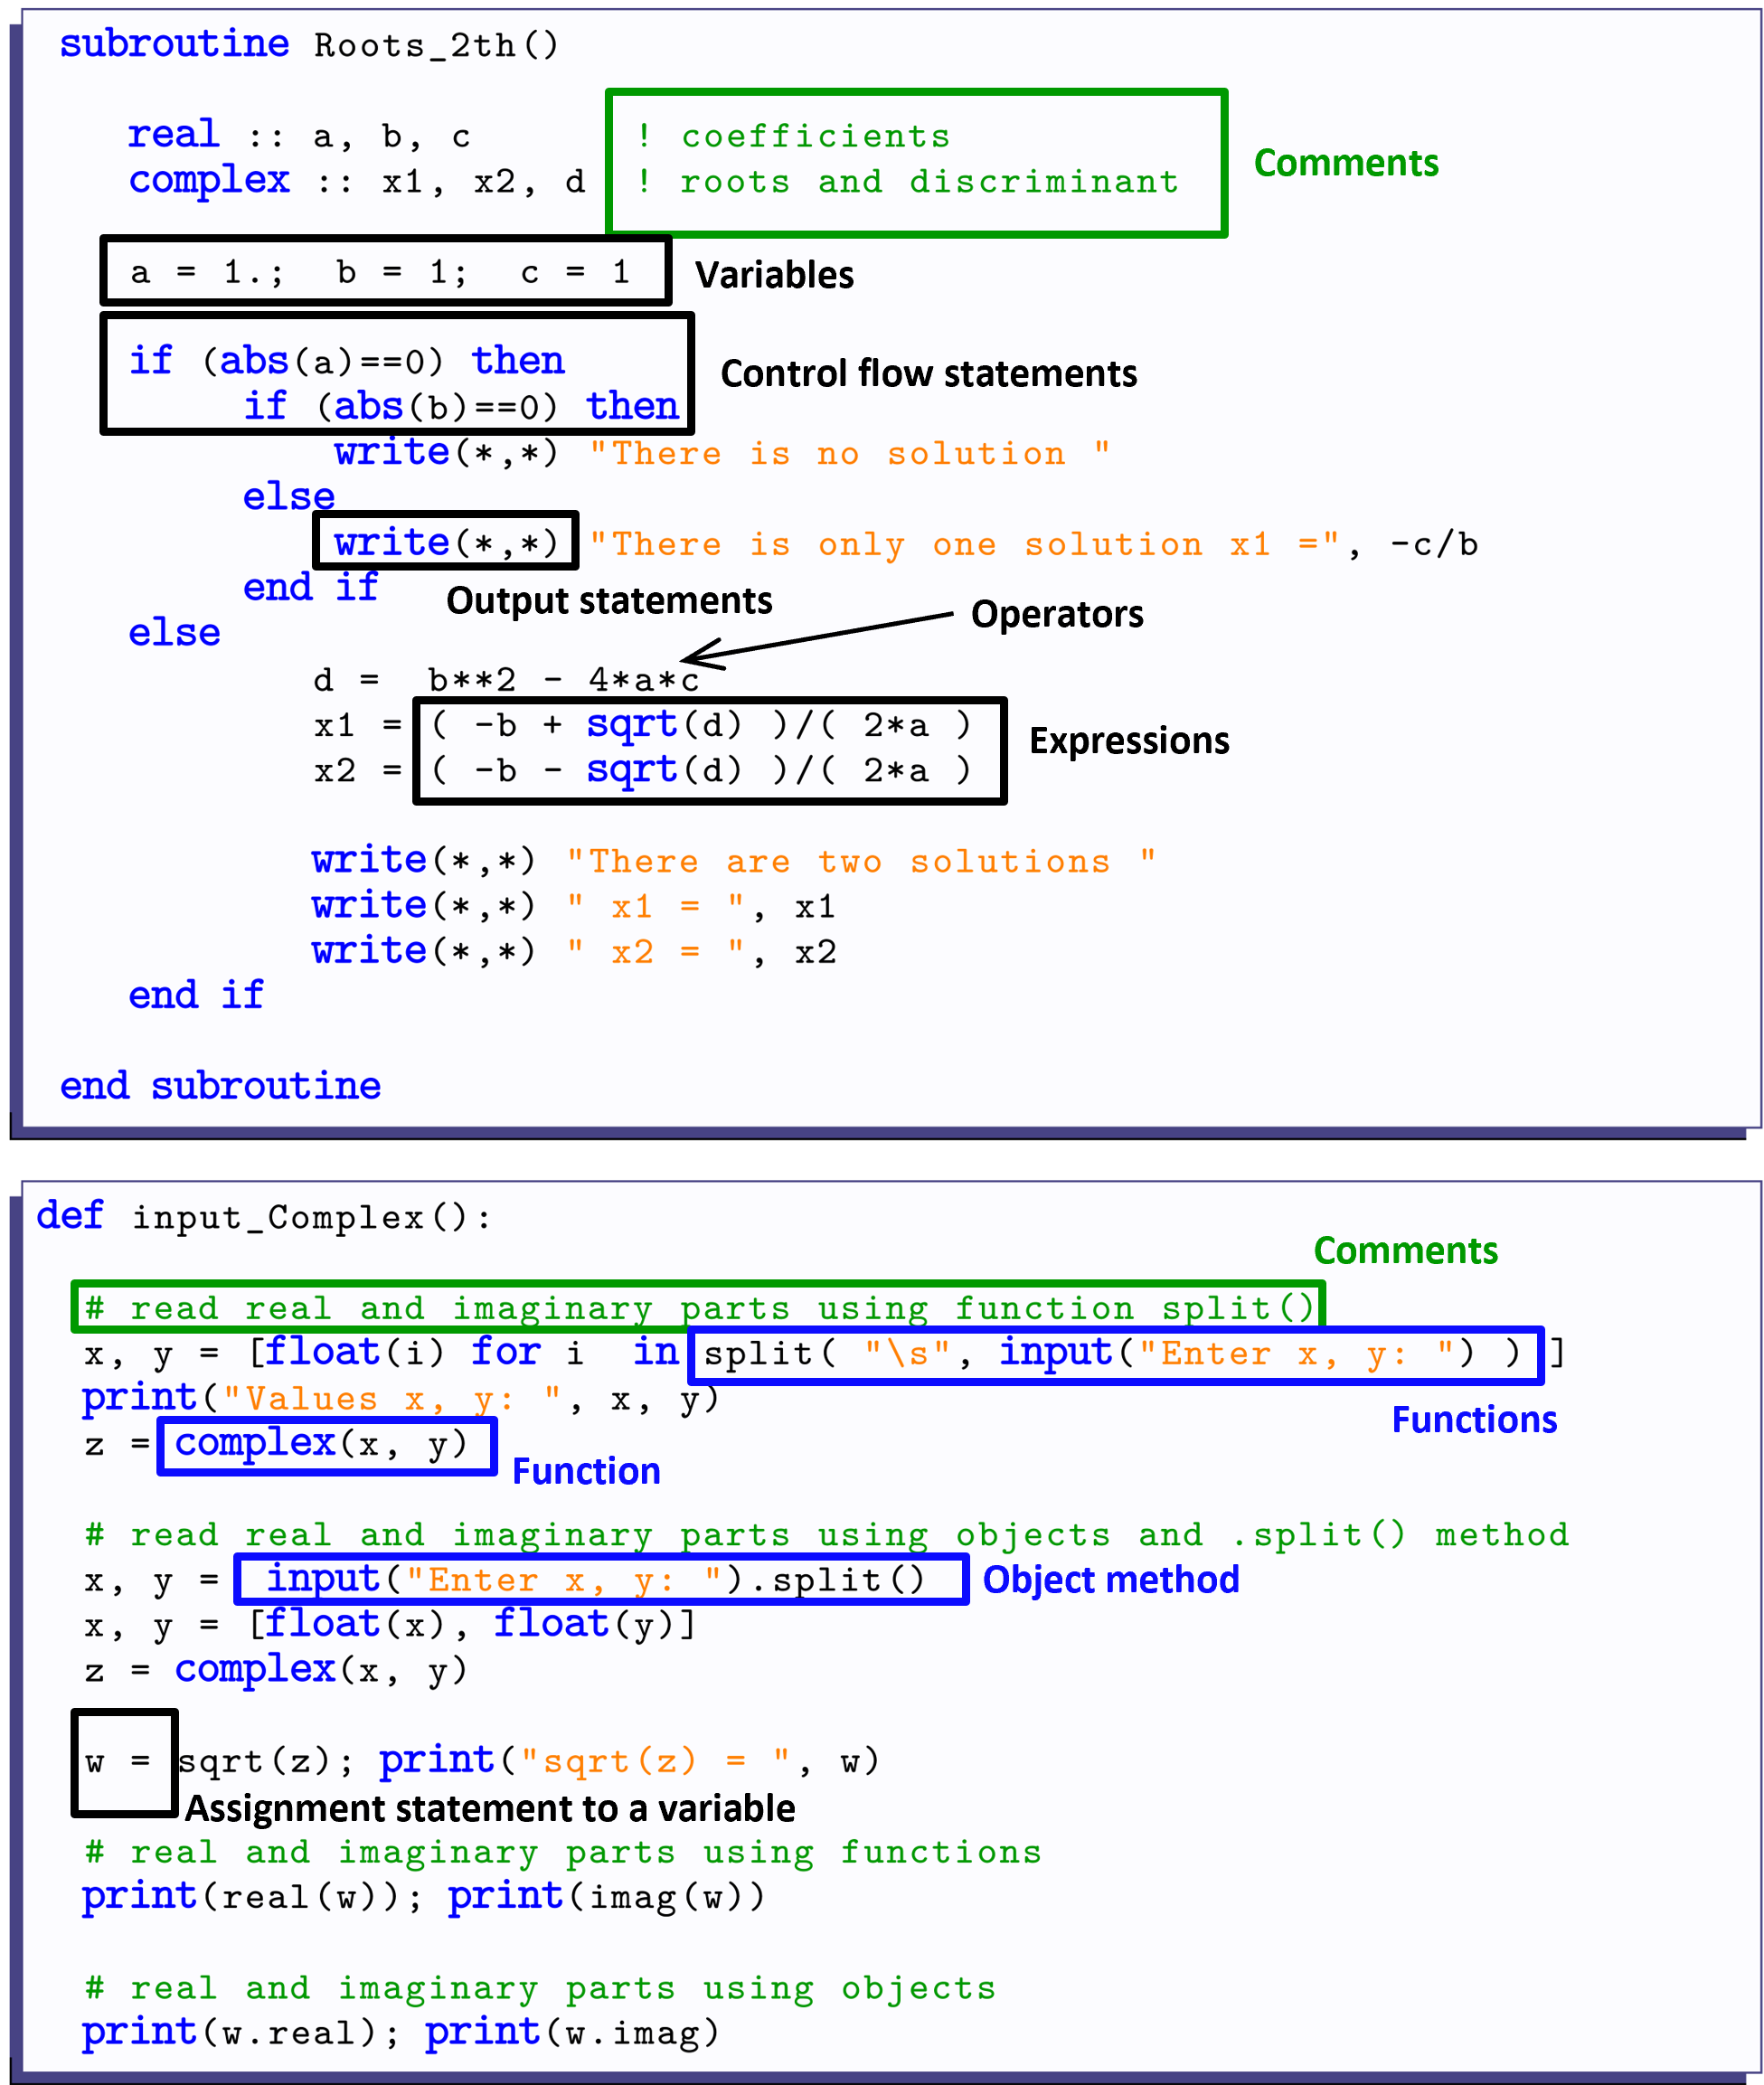
\includegraphics[width=.95\textwidth]{./doc/Figures/components.png}
    \caption{Main building blocks used to code in common programming languages.}
    \label{fig:components}
\end{figure}
\FloatBarrier
 %THIS CODE IS USED TO GENERATE LATER THE IMAGE...
 %\vspace{0.5cm}
 %\renewcommand{\home}{./Fortran/sources/Foundations/Roots} 
 %\lstfor
 %\listings{\home/Roots.f90}{subroutine Roots_2th}{end subroutine}{}
 %
 %\renewcommand{\home}{./Python/sources/Foundations/Data_type} 
 %\lstpython
 %\listingsp{\home/data_type.py}{def input_Complex}{w.imag}{}










%MORE:
%Input: getting data and commands into the computer
%Output: getting your results out of the computer

%Libro FORTRAN: Programación Multicapa

%Most important basic elements for programming languages are:
%Programming Environment
%Keywords
%Input and Output Operations

%Functions
%A function is a statement that returns a value. For example, the function InputBox() returns the value of its dialog text field.
%Objects
%An object is a program “building block” entity. It can be visible, like a Button control, or invisible like a Timer control.
%Properties
%A property is a characteristic of an object. For example, the property Btn.Text is the Text property of the Btn object.
%Methods
%A method is an action that an object can perform. For example, the method Btn.Click() is the Click method of the Btn object.



%The assignment statement \texttt{v = 3*5 + 2} becomes the bottleneck of programming languages in the sense that a program is mainly concerned 
%with the flow of assignments of single variables (imitating single words). 
%By executing assignments many times, maybe altering subscripts (imitating memory addresses), 
%the program ends up with the result stored in a variable (imitating the storage in memory). 
%Furthermore, this assignment statement splits the programming languages into two worlds: 
%a world of expressions with strong algebraic properties (\texttt{3*5 + 2}) and a world of statements with few mathematical properties (\texttt{v =}).



    \section{Data types and their operators}
    
Several objects are used to build the different branches of mathematics; numbers, operations, functions, sets, vectors, matrices, tensors and a large etcetera. 
Let's review here the formal definition of some objects that later are represented in programming by means of the data types. 

In mathematics, the numbers are usually classified into sets according to their nature.
The set of \textbf{integers} $\mathbb{Z}$ includes the number zero (0), the natural numbers ($\mathbb{N} = \{ 1,2,3,... \}$) and their additive inverses ($\{ -1,-2,-3,... \}$), the negative numbers.
The set of \textbf{real} numbers ($\mathbb{R}$) includes any number identified with a point on the real number line.
$\mathbb{R}$ includes both the set of rational numbers ($\mathbb{Q}$) and the set of irrational numbers.
Finally, the \textbf{complex} numbers ($\mathbb{C}$) extends the real numbers using the imaginary unit, an element satisfying the equation $i^2 = -1$, which does not have solution among the reals.
Once introduced the imaginary unit, every complex number can be expressed as $a+bi$ where $a,b\in\mathbb{R}$. 

The fact that a number belongs to one or another set is not only important from the classification point of view.
It also comes with a long list of derived consequences which are essential to build mathematics. 
Let's take for example $\mathbb{Z}$ equipped with the usual \textbf{arithmetic operations} of addition and multiplication and the usual ordering. 
Automatically we can assert that for any $a,b\in\mathbb{Z}$, $a\cdot b\in\mathbb{Z}$ and $a+b\in\mathbb{Z}$.
Also, we do not have to worry about the order to operate them since $a+b=b+a$ and $a\cdot b = b\cdot a$.
To mention other results, for $a,b>0$ then $a+b>0$, $a+b>a$, $a+b>b$, $a\cdot b>0$, $a\cdot b\geq a$, $a\cdot b\geq b$, the equation $a+x = 0$ has a unique solution $x\in\mathbb{Z}$, etc.

From the axioms some properties emerge and other properties are built on these until a whole theory around the integers is built.
The same happens with $\mathbb{N}$, $\mathbb{R}$, $\mathbb{C}$, etc. 
When we use these mathematical objects in a computer, 
it's not only the elements of the set but also
all the properties and results derived. 

However, the arithmetic operators are not the only essential operators in mathematics, 
in the context of ordered sets like $\{\mathbb{R}\}$ or $\{\mathbb{Z}\}$,
any two elements can be compared with the usual ordering, 
which is derived from the 
conventional counting and measuring order on $\mathbb{R}$. 
The \textbf{relational operators} are used to compare any two numbers. 
Both numbers could accomplish with some of the following comparisons: 
equals operator $x = y$, not equal $x\neq y$, less than $x < y$, greater than $x > y$, less or equal than $x \leq y$ and greater or equal than $x\geq y$. 
Notice that the complex numbers do not have the structure of an ordered field and then, these operators are not useful in this context. 


\newpage
Jumping to the context of Boolean algebra, the same principle applies.
However, now the elements to consider are the truth values: \textit{true} and \textit{false}, instead of numbers.
In addition, the basic operations between these elements are conjunction (and), disjunction (or) and negation (not) 
instead of binary operations like addition and multiplication.
These operations allow to combine one or more mathematical statements to create a new one 
and are usually represented by the \textbf{logical operators}.
Given the statements $P$ and $Q$:
\begin{enumerate}[noitemsep]
    \item Conjunction of statements: $P \land Q$ is true when both $P$ and $Q$ are true.
    \item Disjunction of statements: $P\lor Q$ is true when at least $P$ or $Q$ is true.
    \item Negation of a statement: $\neg P$ is true only when $P$ is false.
    \item Implication or conditional: If $P$ then $Q$, $P\to Q$ is false only when $P$ is true and $Q$ is false. 
    \item Equivalent: $P = Q$ or $P \iff Q$ is true if both functional arguments have the same logical value
    \item Non-equivalent: $P \neq Q$ is true if both functional arguments have different logical value
\end{enumerate}
%More than one operator can be used together in an statement building a compound operator.


 

%PROGRAMMING
As a need of representing these essential mathematical sets in the computer, data types are used. 
Each constant, variable, array or function in a language has an intrinsic data type associated, a set to which they belong. 
In the same way, the mentioned \textbf{arithmetic, comparison and boolean operations} are reproduced in the programming language 
so the whole potential of the algebraic structures are transmitted to the computer. 
Hence, the data type decides, among other things, the allowed values that the entity can have and the set of operations that can be performed with them.

Roughly speaking, a value $n\in \mathbb{Z}$ is stored in an \texttt{integer}, 
$x\in \mathbb{R}$ is stored in a \texttt{real} and 
$z\in \mathbb{C}$ is stored in a \texttt{complex} variable.
Many nuances to the equivalence between the programming concept and the mathematical abstraction 
for integers and reals are treated in the Part \ref{PartII} of this book. 

The \texttt{logical} type gets the two possible values of the Boolean algebra; \texttt{True} and \texttt{False}. 
Finally, the \texttt{character} type can store strings with ASCII (American Standard Code for Information Interchange) characters which includes alphanumeric, symbols and sign characters.

Programming languages usually have built-in all the needed operations through \textit{operators} in their syntax,
hence, each of them has a reserved symbol or keyword.
From a general perspective, 
they behave similarly to functions (also treated in this book), 
but they differ in the syntax or the semantics. 
Furthermore, sometimes the language allows the users to create new operators 
or add meanings to existing ones similarly to functions. 





        \newpage
        \subsection*{Fortran code}
        \vspace{-.5cm}
Fortran provides five intrinsic data types:
\begin{itemize}[noitemsep]
    \item Numeric nature: \texttt{integer}, \texttt{real}, \texttt{complex}. 
    \item Boolean nature: \texttt{logical}.
    \item Text nature: \texttt{character}.
\end{itemize}
Fortran has a \textbf{explicit} data typing, which means that before using any variable, all must be previously declared with a specific type.
The code below shows the declaration and initialization of the five intrinsic data types: 
\vspace{0.5cm}
\lstfor
\renewcommand{\home}{./Fortran/sources/Foundations/Basic operations} 
\listings{\home/Basic_operations.f90}{subroutine Data_types}
{end subroutine}{Basic_operations.f90}

\begin{table}[!h]
    \centering
    \begin{tabular}{|l|l|l|l|}
        \hline
        Data Type  & Operator type & Operator & Meaning \\ \hline
        Numeric & Arithmetic & + & Addition \\ 
        ~ & ~ & \texttt{-} & Subtraction \\ 
        ~ & ~ & \texttt{*} & Multiplication \\ 
        ~ & ~ & \texttt{/} & Division (integers!) \\ 
        ~ & ~ & \texttt{**} & Exponentiation \\ 
        ~ & Relational & \texttt{==}   & Equal to (\texttt{=} not valid!) \\ 
        ~ & ~ & \texttt{/=}   & Not equal to \\ 
        ~ & {\footnotesize (no \texttt{complex})} & \texttt{>}   & Greater than  \\ 
        ~ & {\footnotesize (no \texttt{complex})} & \texttt{<}  & Less than \\ 
        ~ & {\footnotesize (no \texttt{complex})} & \texttt{>=} & Greater or equal to \\ 
        ~ & {\footnotesize (no \texttt{complex})} & \texttt{<=}   & Less or equal to  \\ \hline
        \texttt{logical} & Logical & \texttt{.and.} & Conjunction \\ 
        ~ & ~ & \texttt{.or.} & Disjunction \\ 
        ~ & ~ & \texttt{.not.} & Negation \\ 
        ~ & Relational &\texttt{==}  & Equivalent \\ 
        ~ & ~ & \texttt{/=}   & Not equivalent \\ \hline
        \texttt{character} & Character & \texttt{//} & Concatenate \\ 
        ~ & Relational & \texttt{==,/=,>,>=,<,<=} & order ASCII table \\ \hline
    \end{tabular}
\end{table}

%We don't tell the options .EQ., .NEQ., etc.
%Neither the .eqv. and .neqv. in logical



        \newpage 
        \subsection*{Python code}
        \vspace{-.5cm}
The same five data types (also known as primitive data types) are built-in in Python:
\vspace{-0.2cm}
\begin{itemize}[noitemsep]
    \item Numeric nature: \texttt{int}, \texttt{float}, \texttt{complex}. 
    \item Boolean nature: \texttt{bool}.
    \item Text nature: \texttt{str}.
\end{itemize}
\vspace{-0.2cm}
Since Python is mainly an implicit typing language we don't declare the type of any variable and just initialize it.
The following program shows an example of the initialization of the five data types we can find: 
%\vspace{0.5cm} 
\renewcommand{\home}{./Python/sources/Foundations/Data_type} 
\lstpython
\listingsp{\home/data_type.py}{def data_types}
{string}{data_type.py}

\begin{table}[!h]
    \centering
    \begin{tabular}{|l|l|l|l|}
        \hline
        Data Type  & Operator type & Operator & Meaning \\ \hline
        Numeric & Arithmetic & + & Addition \\ 
        ~ & ~ & \texttt{-} & Subtraction \\ 
        ~ & ~ & \texttt{*} & Multiplication \\ 
        ~ & ~ & \texttt{/} & Division \\ 
        ~ & ~ & \texttt{**} & Exponentiation \\ 
        ~ & ~ & \texttt{\%} & Modulus \\
        ~ & ~ & \texttt{//} & Floor division \\
        ~ & Relational & \texttt{==}   & Equal to (\texttt{=} not valid!) \\ 
        ~ & ~ & \texttt{!=}  & Not equal to \\ 
        ~ & {\footnotesize (no \texttt{complex})} & \texttt{>}  & Greater than  \\ 
        ~ & {\footnotesize (no \texttt{complex})} & \texttt{<}  & Less than \\ 
        ~ & {\footnotesize (no \texttt{complex})} & \texttt{>=}  & Greater or equal to \\ 
        ~ & {\footnotesize (no \texttt{complex})} & \texttt{<=}   & Less or equal to  \\ \hline
        \texttt{bool} & Logical & \texttt{and} & Conjunction \\ 
        ~ & ~ & \texttt{or} & Disjunction \\ 
        ~ & ~ & \texttt{not} & Negation \\  
        ~ & Relational &\texttt{==} & Equivalent \\ 
        ~ & ~ & \texttt{!=}  & Not equivalent \\ \hline
        \texttt{str} & Character & \texttt{+} & Concatenate \\ 
        ~ & {\footnotesize needs \texttt{int}} & \texttt{*} & Repetition \\ 
        ~ & ~ & \texttt{in} & Membership \\
        ~ & ~ & \texttt{not in} & Not membership \\
        ~ & Relational & \texttt{==,/=,>,>=,<,<=} & order ASCII table \\ \hline
    \end{tabular}
\end{table}


%Furthermore, while some programming languages allow the use of some data types as if they were a different type (weak typing) others does not (strong typing). 

        \subsection*{Operators}

The operators presented in the tables above are now coded into some examples. 
In the first example we consider a well known equality, the Euler's identity:
$$
e^{i\pi}+1 = 0
$$
In the second one we consider a simple inequality and check the fact that inequalities 
must reverse their sign when both sides are multiplied or divided by a negative value. 
For a given $x,y\in\mathbb{R}$ with $x\leq y$ it is clear that:
$$
-x \geq -y
$$
In the third example the string \texttt{abcdef} is compared alphabetically with \texttt{abcdeg}. 

\vspace{0.5cm}
\lstfor
\renewcommand{\home}{./Fortran/sources/Foundations/Basic operations} 
\listings{\home/Basic_operations.f90}{subroutine Operators}
{end subroutine}{Basic_operations.f90}

\vspace{0.5cm} 
\lstpython
\renewcommand{\home}{./Python/sources/Foundations/data_type} 
\listingsp{\home/data_type.py}{def Operators}{abc}{data_type.py}







    \newpage
    \section{Assignment operator}
The assignment operator is different from the rest of operators in the sense that its 
definition does not come from pure mathematics, it is not related to the mathematical equality 
but related to the assignment statement. 
We have seen that the variables are built by 
a memory storage location tagged with a symbolic name.
While the name is just a tag to identify the data,
the content of the memory location (value) is the data itself. 
Essentially, this operator sets or re-sets the value stored in that memory location (data) using its name. 

To do that the assignment statement is used: 

\texttt{name = expression}

This statement works from right to left, first the \texttt{expression} on the right is evaluated and
when it is done, the data resulted is charged in the memory location tagged by \texttt{name}.
Actually, for some programming languages it is referenced as the left arrow $\leftarrow$ indicating its purpose.
According to John Backus in his article ``Can Programming Be Liberated from the von Neumann Style?'' 
this operator splits the programming languages into two worlds: 
a world of expressions with strong algebraic properties \texttt{expression} and 
a world of statements with few mathematical properties \texttt{name =}.
\vspace{0.5cm}
\lstfor
\listings{./doc/Figures/assignment.f90}{x}{12}{assignment.f90}

%Several variations of the assignment operator are sometimes defined in languages like Python. 
%For example, 
%an operator that adds the right side operand with the left side and then assign the result to the left operand: \texttt{+=}.
%Also, an operator that multiplies the right operand with the left operand and then assign the result to left operand: \texttt{*=}.
%Like this, the following options are allowed: \texttt{-=}, \texttt{/=}, \texttt{\%=}, \texttt{\^{}=}, \texttt{//=}, \texttt{**=}, \texttt{\&=}, \texttt{|=}, \texttt{>>=}, \texttt{<<=}. 






    \newpage
    \section{Control Flow statements}
In order to translate the steps of an algorithm to the programming language 
and essentially manage the flow of data, the control flow statements are needed. 
All the statements in a program are executed from top to bottom but 
the control flow statements modify this behaviour by including decisions, 
loops, branches, separate block executions, etc.
Let's review some essential statements commonly used, 
specially in imperative programming languages 
(we will delve into the concepts of imperative and declarative languages later in this book).


        \subsection{Conditionals}
        \vspace{-0.3cm}
The conditionals are used to separate the flow into branches depending on logical conditions. 
Some statements are executed if a logical expression is evaluated as \texttt{true} and others if it is evaluated as \texttt{false}.

An \texttt{if - then - else} structure is used to evaluate first the condition between parenthesis and execute some statements if it's \texttt{true}.
If the condition is evaluated as \texttt{false} then the statements within the \texttt{else} statement are executed. 
Although \texttt{else} is optional, we strongly recommend to include it in every conditional structure to ensure that at least one of the branches is executed. 
If it seems to be not necessary then write just an error message within the \texttt{else} (see examples). 
A conditional is used to code the absolute value of a number in the examples below. 

The structure \texttt{if - elseif - else} works in the same way, however it allows more than two branches in the same structure. 
From top to bottom all the conditions are evaluated, if one condition is \texttt{false} it jumps to check the following one. 
In the moment that one condition is \texttt{true}, their statements are executed and the structure exited without checking the rest. 
If neither condition is met, the \texttt{else} block of code is executed.
As an example let's compare two integers $a$ and $b$. 

Fortran implements a third kind of conditional, the \texttt{case} structure. 
It executes a block of statements depending on the value of an \texttt{integer} or \texttt{character} expression.
All the Fortran menus in this book are coded using this structure. 
Consider for example the menu of Foundations: 
the user introduces an integer which is stored in \texttt{option} and 
\texttt{select case(option)} is executed accordingly. 
If \texttt{option} is \texttt{2}, the statements under \texttt{case(2)} are executed. 

Notice the differences between both languages. 
In Python the indentation rules must be strictly followed, 
the colon symbol is used before starting the body of the conditional and 
the keywords are \texttt{if}, \texttt{elif}, \texttt{else}.
In Fortran, instead of indentation, the \texttt{end} statement indicates where the body of the conditional ends and 
the keywords are \texttt{if}, \texttt{elseif}, \texttt{else}.


            \newpage
            \subsubsection*{Fortran code} 
            %\vspace{0.5cm}
            \lstfor
            \renewcommand{\home}{./Fortran/sources/Foundations/Basic operations} 
            \listings{\home/Basic_operations.f90}{else conditional}
            {end subroutine}{Basic_operations.f90}
        
        
            \subsubsection*{Python code}
            %\vspace{0.5cm} 
            \lstpython
            \renewcommand{\home}{./Python/sources/Foundations/data_type} 
            \listingsp{\home/data_type.py}{else conditional}{Error}{data_type.py}




        \newpage
        \subsection{Loops}

Loops are used to repeat a bunch of statements cyclically, whether it is executed 
a fixed number of times, 
until a condition is reached or 
maybe up to infinity. 
Typically, the statements inside the loop are executed and then some condition is checked.
Depending on this condition (\texttt{true} or \texttt{false}) the bunch of statements starts again from the beginning or
the loop is exited and the next instruction outside the loop is executed. 

Two basic types of loops are usually used depending 
if the number of iterations is explicitly known or 
it is not but a stop condition is known. 
In the first case, an index controls the loop: it usually has start and stop values and sometimes the increment in each iteration is specified.
Notice that this index cannot be modified inside the loop.
In the second case the number of iterations is not determined beforehand but 
the loop finishes once a condition is evaluated as \texttt{false}. 
This conditions is usually determined by some variables modified inside the loop.

However, some keywords positioned inside a loop can be used to transfer 
some control of the loop execution to the statements inside. 
\begin{itemize}
    \item Use \texttt{exit} in Fortran or \texttt{break} in Python to finish its execution and skip to the next code after the loop. 
    Notice that these statements are usually positioned within a conditional so the loop is finished if the condition is \texttt{true}.        
    \item Use \texttt{continue} in Python to end the current iteration of the loop but continue with the following iteration. 
\end{itemize}

In the examples below we first compute the factorial of a number $n$, $n!$.
Since we know the number of multiplications to perform (given by \texttt{n}) we can use a 
\texttt{do} loop in Fortran and 
\texttt{for} loop in Python.
Notice that in both cases the multiplication stops when multiplying by 2, 
while in Fortran this is expressed by the stop value 2 (\texttt{n, 2, -1}) (sequence $(n, n-1, n-2,...,2)$), 
in Python the \texttt{range} function does not take the stop value at any moment in the sequence
so it has to be expressed as \texttt{range( n, 1, -1 )} (sequence $(n, n-1, n-2,..., 2)$).

Later, the Newton-Raphson method is used to find a good approximation for one root of $f(x) = 3x^3-x^2$. 
We do not know the amount of iterations needed to find the root but we can set as condition that 
the distance between two successive approximations, $|x_{n+1} - x_n|$ is less than $0.00001$ so, while this error condition 
is higher than our threshold, the loop continues iterating.

Finally notice the differences between both languages. 
In Python the indentation rules must be strictly followed and the colon symbol is used before starting the body of the loop.
In Fortran, instead of indentation, the \texttt{end} statement indicates where the body of the loop ends. 


            \newpage
            \subsubsection*{Fortran code} 
            \vspace{0.5cm}
            \lstfor
            \renewcommand{\home}{./Fortran/sources/Foundations/Basic operations} 
            \listings{\home/Basic_operations.f90}{Flow_structures}
            {One root of}{Basic_operations.f90}
            
            
            \subsubsection*{Python code}
            \vspace{0.5cm} 
            \lstpython
            \renewcommand{\home}{./Python/sources/Foundations/data_type} 
            \listingsp{\home/data_type.py}{def Flow_structures}{One root of}{data_type.py}



    \newpage 
    \section{Example: Roots of a second degree equation} 
In this section all of the concepts presented above are put into practice, 
a program to obtain the roots of a second order equation is presented:  
$$
a x^2 + b x + c = 0, \qquad \forall \ a, b, c \in \mathbb{R}.
$$
The fundamental theorem of algebra states that every  Nth order polynomial has N complex roots. 
If the coefficients are real, then the roots are complex conjugate.
Dividing the above equation by $ a $ an looking for a perfect square, 
the following equation is obtained: 
$$
\left( x + \frac{b}{2a} \right)^2 - \frac{b^2 }{ 4 a^2} + \frac{c}{a} = 0. 
$$
Solving the unknown $x$, the well known formula for the roots is obtained: 
\begin{equation}
    x_{1,2} = \frac{ - b \pm \sqrt{ b^2 - 4 a c }  }{ 2 a  }  
    \label{x12}
\end{equation} 
If the discriminant $ d = b^2 - 4 a c $ is less than zero, roots become complex. 
In the following code, complex solutions given by (\ref{x12}) are implemented. 
Note that the discriminant $ d $ was defined as a complex variable to avoid maths problems 
when the discriminant is negative. Whereas negative numbers do not have real square roots, 
they have a value within the set of complex numbers. 

\vspace{0.5cm}
\renewcommand{\home}{./Fortran/sources/Foundations/Roots} 
\lstfor
\listings{\home/Roots.f90}{subroutine Roots_2th}{end subroutine}{Roots.f90}


        \newpage 
        \subsection*{Python code}
The same function is presented now coded with Python. Essentially both codes are quite similar, 
however, now data types for variables are not explicitly declared because 
Python automatically declares them. In addition, indentation rules must be strictly followed. 
\vspace{0.5cm} 
\lstpython
\renewcommand{\home}{./Python/sources/Foundations/Roots} 
\listingsp{\home/Roots.py}{from}{output}{Roots.py}








% -----------------------------------  UNTIL   HERE BASICs  -----------------------------------













    \newpage
    \section{Data structures} 
\vspace{-0.5cm}
Numbers and truth values are not the only objects needed to build the different branches of mathematics.
Also sets, vectors, tuples, matrices, tensors or sequences are used in the context of algebra, calculus or set theory.
Let's review now the formal definition of the objects that are represented in programming by arrays, sets, tuples, lists and dictionaries. 

\begin{enumerate}[noitemsep]
    \item \textbf{Set:} gathering together into a whole of definite, distinct objects of our perception or our thought.
    \item \textbf{Tuples and sequences:} enumerated collection of elements, where repetitions are allowed and order matters. 
    While a sequence can be finite or infinite, a tuple is always finite. 
    \item \textbf{Vectors:} elements of a vector space.
    \item \textbf{Matrices:} rectangular arrangement of numbers (or other mathematical objects) distributed in rows and columns.
    \item \textbf{Graphs:} mathematical structures used to model pairwise relations between objects.
    \item \textbf{Array:} an orderly arrangement of similar mathematical objects.
\end{enumerate}

        \subsection*{Set}
\vspace{-0.5cm}
% --------------------------------------------------------------
A \textbf{set}, with the definition given by Georg Cantor within the set theory, 
is a gathering together into a whole of definite, distinct objects of our perception or our thought, 
which are called elements of the set.
The elements of a set can be any mathematical objects: numbers, points in space, geometrical shapes, variables or other sets.
However, every element of the set must be different from the others.
Sets are usually indicated by listing its elements between curly brackets separated by commas (roster notation): $\{\textrm{car, boat, plane}\}$.

Given two sets $A$ and $B$, the following operations can be performed:
\begin{enumerate}[noitemsep]
    \item Union: $A\cup B$ is the set of elements that belong to set $A$, set $B$ or both.
    \item Intersection: $A\cap B$ is the set of elements that belong to set $A$ and $B$.
    \item Difference: $A - B$ is the set of elements that are in $A$ but not in $B$.
    \item Complement: $\overline{A}$ is the set of all elements that are in the universal set $S$ but are not in $A$.
\end{enumerate}
It is interesting to extend the use of propositional logic to the set theory. 
Notice that an element or set do not have a truth value associated, they are not true or false by themselves. 
By including some relational operators, true or false statements can be 
built and used in the context of propositional logic. 
For example, we can say $3.5 \in \mathbb{R}$ which is true. 

\newpage
Given a set $A$, the following operators are used:
\vspace{-.5cm}
\begin{enumerate}[noitemsep]
    \item Membership: $x\in A$ means that $x$ is an element of the set $A$. The opposite operator would be $x\notin A$.
    \item Subset: $A \subseteq B$ means that all elements of $A$ are also elements of $B$.
    \item Superset: $A \supseteq B$ means that all elements of $B$ are also elements of $A$.
    \item Strict subset: $A \subset B$ means that all elements of $A$ are also elements of $B$ but they are not equal.
    \item Strict superset: $A \supset B$ means that all elements of $B$ are also elements of $A$ but they are not equal.
\end{enumerate}
\vspace{-.5cm}

        \vspace{-.5cm}
        \subsection*{Sequence and Tuple}
        \vspace{-.5cm}
% --------------------------------------------------------------
\textbf{Tuples and sequences} are also collections of mathematical objects.
However, a \textbf{sequence} is an enumerated collection, where repetitions are allowed and order matters.
Unlike sets, since the elements follow an order, they can be repeated in different positions of the sequence.
The length of a sequence is its number of elements and could be any finite value or infinite.
A sequence can also be interpreted (and it usually is) as a function whose domain is a countably ordered set like $\mathbb{N}$ 
(denoting the position within the sequence) to the set of elements. 
Sequences are essential in different branches of mathematics, specially in analysis since they are 
the basis for series.
A $n-$\textbf{tuple} is a finite sequence, which means, a finite ordered lists of $n$ elements where $n$ is a non-negative integer.
Notice that $n-$tuples can be represented by an a single dimensional arrangement of $n$ elements.
Sequences and tuples are usually written between parenthesis or square brackets: $[1,3,5,7,...]$.

        \vspace{-.5cm}
        \subsection*{Vector, matrix and tensor}
        \vspace{-.5cm}
%--------------------------------------------------------------
%vectors
A \textbf{vector} is any element of a vector space.
Historically this term was used for geometric vectors, objects that has magnitude and direction.
In a vector space its members are elements of a set and, satisfying some axioms, they can be added together and multiplied by numbers of a given field. 
These axioms are associativity and commutativity of addition, 
existence of identity and inverse elements for addition, 
existence of identity for scalar multiplication, 
associativity of scalar multiplication and 
distributivity for scalar multiplication over scalar and vector additions. 
Vectors are usually enclosed in parentheses: $(x,y,z)$.

%--------------------------------------------------------------
A \textbf{matrix} is a rectangular arrangement of numbers (or other mathematical objects) distributed in rows and columns.
Matrices over a field $\mathbb{F}$ are those where all its \textit{elements} or \textit{entries} belong to the field $\mathbb{F}$.
If $\mathbb{F}$ is $\mathbb{R}$ or $\mathbb{C}$ it conforms real matrices or complex matrices respectively.
It is usually used $\mathbb{F}^{n\times m}$ or ${\cal{M}}^{n \times m} (\mathbb{F})$ to denote 
the set of $n\times m$ matrices with entries in the field $\mathbb{F}$. 
This set, together with the common addition of matrices and the multiplication by numbers (scalars) 
in the field $\mathbb{F}$ also has the structure of vector space. 
Hence, some matrices are also vectors inherited from the vector space structure they present.
Matrices are commonly written with square brackets: $\begin{bmatrix}  1 & 2 & 3 \\  4 & 5 & 6\end{bmatrix}$.

%Tensors are NOT the generalization of scalars, vectors and matrices (no indices, one index, two indices) to an arbitrary number of indices. 
The concept of \textbf{tensor} has different approaches. 
Avoiding the formal definition let's consider here that a tensor can be represented as a potentially multidimensional array.
The elements in this multidimensional array are called scalar components and are denoted by indices with their position in the array.
A tensor is usually denoted by a symbolic name followed by a collection of subscripts where the number of subscripts attached defines the rank of the tensor: $\alpha_{ijkl}$ is a rank 4 tensor

The operations among numbers in the elementary algebra can be extended to vectors, matrices and tensors. 
The addition and subtraction are element wise-operations: 
they are operated on corresponding elements within the respective objects. 
There are also an element-wise multiplication, multiplication by a scalar, 
vector product, dot product, matrix multiplication, transpose, trace, etc.
These operations are covered in greater depth in chapter \ref{chap:matrices}.



        \subsection*{Graphs}
%--------------------------------------------------------------
\textbf{Graphs} in graph theory and discrete mathematics are structures that model pairwise relations between objects. 
A graph is built by a collection of points (vertices) and lines (edges) connecting a subset of them.
Graphs are usually enclosed in parenthesis and indicating the sets of vertices and edges: $G = (V,E)$ where $V = \{a,b,c\}$ and $E = \{\{a,b\},\{a,c\},\{b,c\}\}$. 


        \subsection*{Array}
%--------------------------------------------------------------
We have used the term \textbf{array} (or arrangement) three times: 
a potential representation for tuples or vectors, 
a representation of matrices and a representation for tensors. 
In maths, an array refers to an orderly arrangement of similar 
mathematical objects. From this definition two notions are essential, 
in an array the elements are of the same kind and they are ordered with a specific pattern.

On one hand, notice that sequences or tuples are not defined in terms of vectors in any sense. 
It can happen that a sequence with elements in a field $\mathbb{F}$ 
(whether finite or infinite)
is a vector in the vector space of all sequences with elements in $\mathbb{F}$.
This is because the addition and multiplication by scalars in $\mathbb{F}$ 
can be defined in terms of element wise common addition and multiplication, 
and satisfy the vector axioms, hence, we have a vector space over $\mathbb{F}$. 
It can also happen that some tuples are vectors of finite dimensional vector spaces. 
However, there is no need that their elements belong to a field and hence, no need 
to consider sequences or tuples  as vectors. 

\newpage
On the other hand, vectors are not defined in terms of sequences or tuples.
Notice that vector spaces can be finite dimensional like the commonly used $\mathbb{F}^{n}$ 
(where $\mathbb{F}$ is a field like for example $\mathbb{R}$ or $\mathbb{C}$) or infinite dimensional.
In the first case, $n-$tuples with elements in the field $\mathbb{F}$ are usually used to represent the vectors once a basis has been chosen. 
Hence, tuples are used to represent the vectors in a specific basis but not being the vectors themselves.
As an example, $\mathbb{R}^{2}$ or $\mathbb{R}^{3}$ are vector spaces 
usually represented as 2-tuples and 3-tuples of reals with respect to a given basis.
When $n-$tuples are used to represent the vectors we can use a one-dimensional arrangement of $n$ elements.
In the case of infinite dimensional vector spaces, tuples cannot be used to represent vectors and sequences sometimes can. 
Some examples are the vector space of infinite sequences of real numbers $\mathbb{R}^\infty$ or 
the set of all continuous real valued functions on $[0,1]$.
It is clear then that some vectors could be seen as tuples, others as sequences and others in neither of these forms. 
However, again there is no need to define 
vectors in terms of these objects since it is not the general situation. 

As a conclusion, even vectors, matrices, tensors, sequences and tuples being different mathematical objects, 
under some specific conditions they can be represented by arrays.

%--------------------------------------------------------------
Let's see some basic examples of these structures in physics and mathematics:
\vspace{-.5cm}
\renewcommand{\arraystretch}{1.5} % Default value: 1
\begin{table}[!h]
    \centering
    \begin{tabular}{|l|l|l|}
        \hline
        \textbf{Data Structure}  & \textbf{Example}  & \textbf{Description}  \\ \hline
        Set  & $\mathbb{N}$ & Natural numbers \\ \hline
        Tuple  & $(x,y)$ & Cartesian coordinates \\ \hline
        Sequence  & $[1,1,2,3,5,8,13,21,...]$ & Fibonacci sequence \\ \hline
        Vector  & $\vec{v} = (\dot{x},\dot{y},\dot{z})$ & Velocity vector \\ \hline
        Matrix  & $H(f) = \left[ \partial^2f / \partial x_i\partial x_j \right]$  &   Hessian matrix   \\ \hline 
        ~  & ~  &   ~   \\[0pt]
        Tensor & $\sigma_{ij} = \left[{\begin{matrix}
                \sigma _{11} & \sigma _{12} & \sigma _{13} \\
                \sigma _{21} & \sigma _{22} & \sigma _{23} \\
                \sigma _{31} & \sigma _{32} & \sigma _{33} \\
        \end{matrix}}\right]$ & Stress tensor  \\
        ~  & ~  &   ~   \\[0pt] \hline
        Graph  & $(\{a,b,c\}, \{\{a,b\},\{b,c\},\{c,a\}\})$ & Cycle graph  \\ \hline
    \end{tabular}
\end{table}

We saw in previous sections that the data type of an object decides, among other things, 
the allowed values that it can have and 
the set of operations that can be performed with them. 
The same applies to data structures, each structure can take specific values and 
can be operated with a different bunch of operators.






        \newpage
        \subsection*{Fortran code}
        
        In a programming language all these objects are represented by different data structures.
        Fortran does not include sets or graphs, but tuples, sequences, vectors, matrices and tensors are represented with arrays. 
        
            \subsubsection*{Array}
            Similar to what happens with scalar variables or constants, 
            each array has a data type, which indicates the data type of the elements within the array.
            In the following code a one-dimensional array with three components is declared and initialized with the values $\vec{v} = (1,2,3)$. 
            Notice that arrays in Fortran are declared enclosed in square parenthesis:  
            \vspace{0.5cm}
            \lstfor
            \renewcommand{\home}{./Fortran/sources/Foundations/Basic operations} 
            \listings{\home/Basic_operations.f90}{subroutine Data_structures}
            {end subroutine}{Basic_operations.f90}

        \newpage
        \subsection*{Python code}
        
        Python has built-in the structures of sets and dictionaries (that can emulate graphs). 
        The mathematical tuples, sequences, vectors, matrices and tensors are represented with arrays, which are available in the library \texttt{NumPy}. 
        In addition, Python has tuples and lists built-in, however, tuples does not have a direct correspondence with its mathematical description. 
        From a general perspective, sets, tuples, lists and dictionaries are used to store collections of data.
        Their elements can be of any type for lists, tuples and dictionaries: 
        strings together with integers and reals, 
        lists nested in lists, tuples within lists, etc. 
        However, sets and ranges present some exceptions to consider in the elements they gather.
        \begin{itemize}[noitemsep]    
            \item Set nature: \texttt{set}, \texttt{frozenset}.
            \item Sequence nature: \texttt{list}, \texttt{tuple}, \texttt{range}.
            \item Array nature: \texttt{array}.
            \item Mapping nature: \texttt{dict}.
        \end{itemize}
        %MATEMATICAS:
        %List/Sequence: enumerated collection of objects in which repetitions are allowed and order matters. USUALLY INFINITE
        %Tuple: enumerated collection of objects in which repetitions are allowed and order matters. ALWAYS FINITE
        
        %PROGRAMMING PYTHON:
        %List/Sequence: enumerated collection of objects in which repetitions are allowed and order matters. ONLY FINITE IS POSSIBLE
        %Tuple: Same as list but it can not change (programming concept not related to maths)
        
        
            \subsubsection*{Set}
            \vspace{-.5cm}
            A \texttt{set} in Python takes the same meaning as the mathematical object: a collection of any type of data that 
            i) is unordered and 
            ii) do not allow duplicate values. 
            In a set, all that matters is whether each element is in it or not, so the ordering of the elements is irrelevant.
            Furthermore, two equal elements, since they are not ordered, could not be distinguished between them. 
            While a set is mutable (remove or add elements is allowed), a \texttt{frozenset} is an immutable set, once created, its content can not be modified. 
            Sets cannot contain lists or dictionaries since they are unhashable structures (they do not contain any hash value that never changes during their lifetime).
            Following the roster notation, a set is expressed by listing its elements between curly brackets and separated by commas.
            \vspace{0.3cm} 
            \lstpython
            \renewcommand{\home}{./Python/sources/Foundations/data_type} 
            \listingsp{\home/data_type.py}{Set}{remove}{data_type.py}
            
            %Notice that the sets \texttt{ \{``car'', 5, 6.7, 1 + 1j\} } and \texttt{\{5, 1 + 1j, 6.7, ``car'', 5\}} 
            %are the same since repetition and order change do not modify it.
            
            \subsubsection*{List and Tuple}
            \vspace{-.5cm}
            A \texttt{list} in Python is a collection of data characterised by being 
            i) ordered: the position within the list is kept, 
            ii) allow duplicates: items can appear more than one time in the list and  
            iii) changeable: change, add, and remove items are allowed.
            In a list, the difference between any two elements comes with the index within the list.
            Lists are written using square brackets \texttt{[]} with comma-separated values.
            
            A \texttt{tuple} does not take the mathematical definition of tuple.
            In Python a tuple is the same as a list with the difference that tuples are unchangeable. 
            Hence, a tuple is characterised by being 
            i) ordered: the position within the tuple is kept, 
            ii) allow duplicates: items can appear more than one time in the tuple and  
            iii) unchangeable: once created, it can not be modified.
            For tuples, Python allocates the required memory once and not reallocates it. 
            This becomes a more memory efficient strategy to follow when the data is going to be immutable.
            Tuples are written using parenthesis \texttt{()} with comma-separated values.
            \vspace{0.1cm} 
            \lstpython
            \renewcommand{\home}{./Python/sources/Foundations/data_type} 
            \listingsp{\home/data_type.py}{Tuple}{false}{data_type.py}
            
            %No ponemos subset como operacion porque solo lo computa si estan ordenados de la misma forma 
            
            \vspace{-.5cm}
            \subsubsection*{Range}
            \vspace{-0.5cm}
            A \texttt{range} structure is a strictly increasing or decreasing sequence of integers. 
            It is more efficient than a list or tuple since only generates the values 
            of the sequence when are needed and do not store any values in memory. 
            For \texttt{range(start, stop, step)} all its arguments are integers, 
            \texttt{start} and \texttt{step} are optional.
            If only \texttt{stop} is specified the sequence starts in \texttt{0} and do not include the \texttt{stop} value itself.            
            \vspace{0.1cm} 
            \lstpython
            \renewcommand{\home}{./Python/sources/Foundations/data_type} 
            \listingsp{\home/data_type.py}{Range}{Stops in}{data_type.py}
            
            \subsubsection*{Array}
            In Python array structures are not built-in, however, the library \texttt{NumPy} supports them.
            In the following code a one-dimensional array with three components is declared and initialized with the values $\vec{v} = (1,2,3)$. 
            Notice that the function array is used to declare this structure.
            \vspace{0.3cm} 
            \lstpython
            \renewcommand{\home}{./Python/sources/Foundations/data_type} 
            \listingsp{\home/data_type.py}{Array}{print}{data_type.py}
            
            
            \subsubsection*{Dictionary}
            A dictionary (\texttt{dict}) is a collection of data that stores pairs \texttt{key:value}. 
            It is similar to a set in some sense, it is characterised by being 
            i) ordered: the position is kept (however, in terms of comparison, two dictionaries with same pairs but different order are considered as equals), 
            ii) do not allow key duplicates: the same key can not appear more than once and  
            iii) changeable: change, add, and remove items are allowed.
            It can store any type of data; lists, integers, tuples, ..., and even other dictionaries nested.
            A dictionary is declared by a list of elements separated by commas, 
            enclosed in curly brackets (\texttt{\{\}}) and 
            using a colon (\texttt{:}) to separate each pair. 
            \vspace{0.3cm} 
            \lstpython
            \renewcommand{\home}{./Python/sources/Foundations/data_type} 
            \listingsp{\home/data_type.py}{Dictionary}{a not in F}{data_type.py}





    \newpage
    \section{Iterators}
    \vspace{-.5cm}
In this section, some iterators are presented for 
sets, lists, tuples, dictionaries and even strings in Python. 
Arrays are treated in the chapter \ref{chap:matrices}, however, 
notice now that both Python and Fortran use the indices of each dimension as iterators.
Hence, loops with different indices are used to reference any element within the array.

Sets, lists, tuples, ranges, dictionaries and strings, 
they all contain a countable number of elements so 
they are considered iterable data structures. 
Three main strategies can be used to iterate:
\vspace{-.3cm}
\begin{enumerate}
    \item \textbf{Iterating in the elements:} All iterable structures are iterable in their elements, including strings.      
    \item \textbf{Iterating in the index:} While lists, tuples and strings are easily iterable on their indices, 
    sets are not subscriptable (they do not have order) and 
    dictionaries need keys as subscripts and not indices.    
    \item \textbf{Iterate in both the index and the element:} While lists, tuples and strings are easily iterable on their indices, 
    sets are not subscriptable (they do not have order) and 
    dictionaries should be better iterated using their keys.
    \item Dictionaries have two extra methods to iterate: 
    \texttt{for k in D.keys()} to iterate in the keys and
    \texttt{for v in D.values()} to iterate in the values. 
\end{enumerate} 
\vspace{-.3cm}
Notice that the structure \texttt{range()} is used in combination with \texttt{len()} 
to iterate in the index of any other structure. 
The function \texttt{len()} returns the length of the structure and \texttt{range()} 
returns a sequence of numbers between \texttt{0} and the given length.
%\vspace{.2cm}
\lstpython
\renewcommand{\home}{./Python/sources/Foundations/data_type} 
\listingsp{\home/data_type.py}{def iterators}{the values of}{data_type.py}



%Finally, notice that every iterable object can use the \texttt{iter()} method to create an iterator from the data structure and
%the \texttt{next()} method to jump element in the iterator (see \texttt{ite} in the code above).
%Actually, Python is using this kind of iteration behind the more straightforward options seen.
% 
% #ite = iter( ("one", 5, 3.5, 5) )
% #print( next(ite) )
% #print( next(ite) ) #returns StopIteration when no more elements. 
 
 
To access the elements of these iterable objects the square brackets notation is used.
In the example below, the third element of the list \texttt{L} or the tuple \texttt{T}
is obtained. Notice that the indices start always in 0. 
In a similar way, we can access the element with key \texttt{''a''} in the dictionary \texttt{D} 
as shown in the example below.
\vspace{.5cm}
\lstpython
\renewcommand{\home}{./Python/sources/Foundations/data_type} 
\listingsp{\home/data_type.py}{Third element}{with key}{data_type.py}
 
 
We have seen how to manually define these structures, but this is not the only way to do it. 
When our structure is defined by a general term, or it takes a slice from another structure, 
the \textbf{list comprehension} method (an implicit loop iterating in another structure) is used. 
It can be used for lists, tuples, sets, etc. 
Its notation for a tuple is:
\begin{verbatim}
(expression for index in iterable if condition == True)
\end{verbatim}
where \texttt{for}, \texttt{in} and \texttt{if} are the keywords of the notation.
As an example let's generate a set of Pythagorean triples, 
tuples like: 
$$\left(a,b,c\in\mathbb{Z}^+|a^2 + b^2 = c^2\right)$$ 
using the following three equations up to $i = 9$:
\begin{equation}
    \begin{cases}
        a  & = i^2 - 1\\
        b & = 2i\\
        c & = i^2+1
    \end{cases}       
\end{equation}
\vspace{.5cm}
\lstpython
\renewcommand{\home}{./Python/sources/Foundations/data_type} 
\listingsp{\home/data_type.py}{Pyt}{print}{data_type.py}
 
 

 
 
 
 
 
 
 
 
 
 
%FUTURE? 
 
%where??

%Luego hay funciones y metodos de objetos para hacer un monton mas de operaciones de todo tipo. 
%In a set the data can be modified through built-in methods so for example mathematical set operations like union, intersection or difference can be performed.

%future?
%\texttt{ (/ list /) } is not used as constructor.

%enumerate en Python futuro?

%For sets with many elements, especially those following an implicit pattern,
%the list of members can be abbreviated using an ellipsis ``...''.
%For instance, the set of the first thousand positive integers 
%may be specified in roster notation as
%\begin{verbatim}
%    { 1, 2, 3, ..., 1000 }.
%\end{verbatim}

%Derived data types can be created either from intrinsic types or from other derived types previously defined.
%In addition, Python also allows non-primitive data types (explained in this book as data structures)
%and user-defined data structures.

%Let's find in the examples below an approximation to the infinite sum of the sequence: 
%$$
%\left[\sqrt{\frac{n}{n^4+1}}| n\in\mathbb{N}\right]
%$$
%# List, sequence
%print( "Sum sqrt(n/(n**4+1)) = ", sum( [sqrt(n/(n**4+1)) for n in range(10000+1)] ) )

%
%Given the set 
%$\Pi = \{1\leq i\leq 30, i\in\mathbb{N}|\; i \;\textrm{is prime}\}$ 
%and the set 
%$E = \{1\leq i\leq 30, i\in\mathbb{N}|\; i \; \textrm{is even}\}$: 
%$$
%\Pi = \{2, 3, 5, 7, 11, 13, 17, 19, 23, 29\}
%$$
%$$
%E = \{2, 4, 6, 8, 10, 12, 14, 16, 18, 20, 22, 24, 26, 28, 30\}
%$$
%we can check first that the following assertion is false:
%$$
%(1\in P) \land (5\in P)
%$$
%and we can also check the first De Morgan's Law ($\neg (P\lor Q) \iff (\neg P \land \neg Q)$) for the assertions $P = a\in \Pi$ and $Q = a\in E$:
%$$
%\neg (a\in\Pi \lor a\in E) \iff (\neg a\in\Pi \land \neg a\in E)
%$$
%%$$
%%(\neg a\in\Pi \land \neg a\in E) \to   \neg (a\in\Pi \lor a\in E)
%%$$
%
%En el codigo de operadores
%
%P = {2, 3, 5, 7, 11, 13, 17, 19, 23, 29}
%E = {2, 4, 6, 8, 10, 12, 14, 16, 18, 20, 22, 24, 26, 28, 30}
%
%print( "(1 in P) and (5 in P) = ", (1 in P) and (5 in P) )
%print( not(a in P or a in E), "implies", not(a in P) and not(a in E) )












%NOT USED

%In the context of the elementary algebra, some operations are defined for the elements of each of these sets, addition and multiplication.
%Furthermore, the properties of these operations give a ring structure to the integers 
%and a field structure to reals and complex. 
%These properties among others build the structure of ring for the integers and much more properties can be derived.
%Furthermore, when some results are proved for a set with their operations, 
%any other set and operations following the same axioms
%        \subsection*{Arithmetic operators}
%\vspace{-0.5cm}
%For both Fortran and Python the symbols for the main arithmetic operations are:
%\vspace{-0.7cm}
%\begin{itemize}[noitemsep]
%    \item \texttt{+} for the addition operator, 
%    \item \texttt{-} for subtraction,
%    \item \texttt{*} for multiplication,
%    \item \texttt{/} for division and
%    \item \texttt{**} for exponentiation.
%    
%    \vspace{0.3cm}
%    Python also includes the modular arithmetic operators:
%    \item \texttt{//} for the floor division (ONLY PYTHON).
%    \item \texttt{\%} for the modulo operation (ONLY PYTHON).
%\end{itemize}
%
%%(specially important when working with finite fields and cybersecurity)
%%\footnote{It implements the floor function over the result of the division: it returns the greatest integer less than or equal to $x\in\mathbb{R}$.}
%%\footnote{It returns the modulus of the division, its remainder after one number is divided by another.}

%        \subsection*{Relational operators}
%        \vspace{-0.5cm}
%        For both Fortran and Python the relational operators are:
%        \vspace{-0.5cm}
%        \begin{itemize}[noitemsep]
    %            \item \texttt{==} for the \textit{equal to} operator (notice that \texttt{=} is not used for this), 
    %            \item \texttt{/=} in Fortran and \texttt{!=} in Python for the \textit{not equal to} operator.
    %            \item \texttt{>} for the \textit{greater than} operator,
    %            \item \texttt{<} for the \textit{less than} operator,
    %            \item \texttt{>=} for the \textit{greater or equal to} operator and
    %            \item \texttt{<=} for the \textit{less or equal to} operator.
    %        \end{itemize}
%    \vspace{-0.5cm}
%        Historically, Fortran also allows \texttt{.EQ., .NE., .GT., .LT., .GE., .LE.} for the above operators respectively. 

%        
%        \subsection*{Logical operators}
%        \vspace{-0.5cm}
%        In Fortran the logical operators are:
%        \vspace{-0.5cm}
%        \begin{itemize}[noitemsep]
    %            \item \texttt{.and.} in Fortran, \texttt{and} in Python for the conjunction operator, 
    %            \item \texttt{.or.} in Fortran, \texttt{or} in Python for the disjunction operator,
    %            \item \texttt{.not.} in Fortran, \texttt{not} in Python for the negation operator,
    %            
    %            \vspace{0.3cm}
    %            Fortran also includes the following:
    %            \item \texttt{.eqv.} for the equivalent operator (true if both functional arguments have the same logical value, ONLY FORTRAN) and
    %            \item \texttt{.neqv.} for the non-equivalent operator (true if both functional arguments have different logical value, ONLY FORTRAN).
    %        \end{itemize}

%        In Python the logical operators are:
%        \vspace{-0.5cm}
%        \begin{itemize}[noitemsep]
    %            \item  for the conjunction operator, 
    %            \item  for the disjunction operator and
    %            \item  for the negation operator.
    %        \end{itemize}

%        \subsection*{Membership operators}
%        \vspace{-0.5cm}
%        Python allows the membership operators for sets, lists, tuples and dictionary keys:
%        \vspace{-0.7cm}
%        \begin{itemize}[noitemsep]
    %            \item \texttt{in} for the $\in$ operator and
    %            \item \texttt{not in} for the $\notin$ operator.
    %        \end{itemize}        
%      

%
%We mentioned before that a lot of properties are derived from the structure of the integers with the usual addition and multiplication and their properties. 
%Well, in mathematics: rings, fields, groups, vector spaces and more algebraic structures 
%are built with the following ingredients:
%\vspace{-0.6cm}
%\begin{enumerate}[noitemsep]
%    \item A nonempty set $A$.
%    \item Some operations on $A$.
%    \item A finite set of axioms that these operations must satisfy.   
%\end{enumerate}
%\vspace{-0.6cm}
%We can consider for example the set of reals together 
%with the operations of addition and multiplication 
%and the following axioms: 
%associativity and commutativity of addition and multiplication, 
%existence of additive and multiplicative identity,
%existence of additive and multiplicative inverses and
%distributivity of multiplication over addition.
%Then, the field $\{\mathbb{R}, +, \times\}$ is built. 
%
%A big amount of consequences are derived from the fact that we are working with a field:
%some equations are proved to have unique solutions, subtraction and division (except by 0)
%can be performed, every Cauchy sequence has a limit, etc. 


  
  
 
 

         
\newpage 
%\chapter{Imperative programming versus declarative programming} 
\chapter{Sum of series. Imperative versus declarative}   \label{chap:impdec}


\section{Introduction}
\vspace{-0.5cm}
A big number of programming languages exist nowadays, all of them covering different features 
in order to fit diverse needs. While a programming languages is focused on the way the 
code is organized, other language gives importance to the dataflow through operations.
Consider as an example the object-oriented paradigm, one of his main features 
is that the data is organized into objects 
that are modified by methods also specified in the object.

%According to these features, the different programming paradigms appear. 
A group of these features define the conceptual framework of the language, its programming paradigm.
Think of it as a group of ideas that describe how to write a program. Some languages are based only on one 
paradigm while others are multi-paradigm so their programs are too.  

A big amount of programming paradigms are commonly grouped into two types: imperative and declarative. 
This chapter covers the difference between both supported on examples of numerical sum series.

In an imperative style, the programmer tells the machine \textbf{how} to perform each task step by step,
hence, an statement describes how to change the state of the program.
However, in a declarative paradigm, the programmer tells the interpreter/compiler \textbf{what} to obtain
and its properties but not the control flow of the process. 



\section{Sum of numerical series} 
One of the main tasks of numerical calculus is to sum numerical series
which appear from approximation of functions to numerical integration. 

The algorithm to sum these series can be done in an iterative way by a sequential machine or von Neumann
machine or concurrently by a bunch of processors.
This first idea allows to introduce the two different paradigms mentioned when trying to write or to implement 
algorithms in different programming languages: imperative paradigm and declarative paradigm. 

Imperative programming is related to an ordered sequence of sentences that allows to obtain the solution
whereas declarative programming is concerned with the specification or the statement of the problem 
no matter the way it is accomplished. 

The following sum series are treated in the Fortran project included with this book:

$$
S = \sum_{n=1} ^{\infty} \frac{ (-1)^{n+1} } { 2^n },  \ \   \ \
S = \sum_{n=1} ^{\infty} \frac{ 1 } { n! },  \ \   \ \
S = \sum_{n=1} ^{\infty} \frac{ 1 } { n^2 }
$$

The first two examples have a good convergence, this means that the general
term $a_n$ tends to zero quickly with  $n \rightarrow \infty$ and few terms must be added 
to get a correct result. 
Then, it is easy to obtain the result of the infinite sum up to a given finite number of digits. 
However, the third example has a poor convergence and some issues must be review to sum it 
in a correct way. The following chapter is dedicated to this third example and the particularities 
that appear when bad convergence series are calculated with a finite precision machine. 


%--------------------------------------------------------------------------------------------
%--------------------------------------------------------------------------------------------
\newpage 
\section{First example with imperative paradigm} 
Let's consider the following summation  as an example to show how the imperative paradigm 
can be implemented. 
$$
S_N = \sum_{n=1} ^{N} \frac{ 1 } { n^2 }
$$
In the following code, the summation is done in an iterative way. 
\vspace{0.5cm}
\renewcommand{\home}{./Fortran/sources/Foundations/Calculus} 
\listings{\home/Examples/Sum_series.f90}{function SummationN_n2}
          {end function}{Sum_series.f90}
          

The result for \texttt{N = 10} is obtained by calling the function in the following way:
\begin{verbatim} 
    write(*,*) " S = ", SummationN_n2( 10 ) 
\end{verbatim}

Notice how the main task to develop (sum a value to the older value of \texttt{S}) is specified to the 
compiler with a loop. Since this function is simple, the imperative style used is easy to read and easy to 
learn for beginners. However, with more complex tasks, the code quickly becomes extensive and difficult 
to follow and maintain.

If you are curious about the need of including \texttt{real(i)} in the denominator of the sum, 
this issue is treated in the section \ref{sec:NumIssues} and also you can take a look 
at the chapter \ref{sec:UndersIntOver}. Just forcing the number \texttt{1.} of the numerator to be real, 
the operations are performed in the reals field so the result is properly calculated, converting the denominator to 
real should not be needed. However, there is another interest in doing that. As a clue, overflow of integers must be avoided. 
    
    
\newpage 
\subsection*{Python code} 
This example can be implemented with Python in a similar way.
Notice that data type for variables (\texttt{S}, \texttt{i} or \texttt{N}) is not explicitly declared, 
Python automatically declares it when a value is assigned. Also, indentation rules are strictly followed and 
there is no need to close structures like loops by means of statements. 
\vspace{0.5cm}
\renewcommand{\home}{./Python/sources/Foundations/Calculus} 
\lstpython
\listingsp{\home/Examples/Sum_series.py}{def SummationN_n2}
          {return}{Sum_series.py}          
\lstfor


\newpage 
\section{First example with declarative paradigm}
Now the same sum is coded with declarative programming. On one hand, the abstraction of 
summation is used for the function \texttt{Sigma\_N}, an easily reusable code has been created and once 
validated it will be used for future similar projects. On the other hand, the general term of the sum 
is independently declared in a different function, hence, if the program specifications change 
(a different sum is needed), updating this code is extremely easy. 

\vspace{0.5cm}
\renewcommand{\home}{./Fortran/sources/Foundations/Calculus} 
\listings{\home/Series.f90}{function Sigma_N}
          {end function}{Series.f90}

\vspace{0.5cm}
\renewcommand{\home}{./Fortran/sources/Foundations/Calculus} 
\listings{\home/Series.f90}{interface}
          {end interface}{Series.f90}

\vspace{0.5cm}
\renewcommand{\home}{./Fortran/sources/Foundations/Calculus} 
\listings{\home/Examples/Sum_series.f90}{function a1}
          {end function}{Sum_series.f90}



The result for \texttt{N = 10} is obtained by calling the function in the following way:
\begin{verbatim} 
    write(*,*) " S = ", Sigma_N( a1, 1, 10 ) 
\end{verbatim}

\newpage
The essence of the declarative programming in this example are the lines:

\texttt{S = sum( [ (a(i), i=i0, N ) ] )} 
 
\texttt{Sigma\_N( a1, 1, 10 )}

Both lines tell the compiler the properties of the solution to be obtained, no matter how the process is done. 
In the first case the intrinsic function \texttt{sum} performs the summation 
of the elements of a Fortran vector by means of an implicit loop from one value to another. The properties of the solution sought are 
of course the limits of the sum (\texttt{i0} and \texttt{N}) and the type of term to be added. 
In the second case, thanks to the created function \texttt{Sigma\_N}, the sum is performed just by declaring the 
general term to add and the limits, the programmer does not need to tell the compiler how to do the summation step by step.

Another ingredient is needed for this example, since the function \texttt{Sigma\_N} admits any general term 
of a series, it needs to know how to communicate with the function that defines that general term \texttt{a1(n)}. 
Through the interface block (intentionally created defining a function from integers to reals) \texttt{Sigma\_N}
knows everything about the dummy arguments used inside the referenced procedure \texttt{a1(n)}. The same procedure 
could be recycled next time a function of the following form is used: 
$$ 
\myfunc{ \texttt{f\_N\_R} }{\mathbb{Z}}{\mathbb{R}}{n}{\texttt{f\_N\_R(n)}} 
$$
\subsection*{Python code}
The same advantages demonstrated with Fortran are visible in Python, 
now the extension and simplicity of the code is even higher due to the characteristics of this language. 
We do not need vectors in Python since lists, the representation of matheamtical sequences, are built-in in the language. 
However, do not forget the implicit assumptions that are made for its statements; 
type and kind of variables, interface between procedures, etc.  
\vspace{0.3cm}
\renewcommand{\home}{./Python/sources/Foundations/Calculus} 
\lstpython
\listingsp{\home/Series.py}{def Sigma_N}
          {return}{Series.py}  
\vspace{0.2cm}
\listingsp{\home/Examples/Sum_series.py}{def a1}
          {return}{Sum_series.py}



%--------------------------------------------------------------------------------------------
%--------------------------------------------------------------------------------------------

\newpage 
\section{Second example with imperative paradigm} 
Let's consider another series summation example with imperative paradigm. 
In this case the result sought is the summation of the infinite terms of the series. 
$$
S = \sum_{n=1} ^{\infty} \frac{ 1 } { n^2 }
$$
In the following code, the summation is done in an iterative way. 
\vspace{0.5cm}
\renewcommand{\home}{./Fortran/sources/Foundations/Calculus} 
\listings{\home/Examples/Sum_series.f90}{function Summation_n2}
          {end function}{Sum_series.f90}

This piece of code performs the summation of as many terms as 
the variable \texttt{S} can significantly sum to itself. 
Once the nth term of the sum is not going 
to modify the value of \texttt{S} due to its finite number of digits, 
the result obtained is the closest value
to the infinite sum that \texttt{S} can hold (with this specific algorithm). 
Then, \texttt{n} is returned indicating the last term calculated. 

The sum must be stopped once the result of \texttt{an} is smaller than the 
smallest number that can be added to \texttt{S}. Then, the result of 
adding \texttt{S + an} is equal to \texttt{S}. Notice that the calculus of \texttt{S}
from one step to the next one is the same to the first example. However, now \texttt{Sn}
is used to compare the value before and after the nth sum. If both values are the same, 
it means that \texttt{an} has not contributed to \texttt{S} and the process is stopped. Also, 
take into account the need of
initializing \texttt{S} and \texttt{Sn} with different values.
 
\newpage
The result of the sum is obtained by calling the function in the following way:
\begin{verbatim} 
    integer :: n
    
    write(*,*) " S = ", Summation_n2( n )
\end{verbatim}


\vspace{0.5cm}

\subsection*{Python code}
The same imperative statements are presented now with Python.  

\vspace{0.5cm}
\renewcommand{\home}{./Python/sources/Foundations/Calculus} 
\lstpython
\listingsp{\home/Examples/Sum_series.py}{modify arguments}
          {return S}{Sum_series.py}
\lstfor





\newpage
\section{Second example with declarative paradigm}  \label{sec:Sigma}
For this example a modification of \texttt{Sigma\_N} is needed: \texttt{Sigma}. Nevertheless, notice the simplicity of the code when 
the existing function \texttt{Sigma\_N} is reused.

For an infinite sum it is more interesting to declare the minimum term to add to the sum (\texttt{eps}) instead of the number of 
terms to sum (\texttt{N}). The programmer does not normally know how many terms are needed to reach a finite number of digits in the result.
However, the allowed error of the result is usually a specification. 
%the minimum term that his result can store in order to calculate it. 
For this reason, \texttt{N} is automatically found by specifying the general term and the 
minimum term to sum with the function \texttt{Tail(a, eps)}. 
Then, \texttt{Sigma\_N} is used to perform the sum as seen in the previous example. 

Once again, the operation is performed by means of a desired properties bunch and not declaring the control flow step by step. 
This strategy increases the capabilities of solving many different problems with the same tools by creating more and more complex functions 
always based on lower level functions (in a hierarchical structure). In this case for example, a new degree of freedom (\texttt{eps}) 
is obtained by using \texttt{Sigma}, which is based on \texttt{Tail} and \texttt{Sigma\_N}. 
This programming paradigm also leads to a reuse strategy, where the next time that a similar task is performed 
in another program, the same functions can be used thereby saving time.


\vspace{0.5cm}
\renewcommand{\home}{./Fortran/sources/Foundations/Calculus} 
\listings{\home/Series.f90}{function Sigma}
          {end function}{Series.f90}

\newpage 
\vspace{0.5cm}
\renewcommand{\home}{./Fortran/sources/Foundations/Calculus} 
\listings{\home/Series.f90}{function Tail}
          {end function}{Series.f90}

Do not forget to declare the same interface block of the first example \texttt{f\_N\_R(x)} and define 
the general term to sum (\texttt{a1} for example), then, the following statements obtain the infinite sum
for a minimum general term of \texttt{eps = 1e-10}:
\begin{verbatim} 
    real :: eps
    
    eps = 1e-10
    write(*,*) " S = ", Sigma( a1, 1, eps ) 
\end{verbatim}




The mathematical support for the function \texttt{Tail} is treated in the section \ref{sec:NumIssues}. 
It is essential to notice three issues:

\begin{enumerate}
    \item This function is written for good convergence series since its definition is based on 
    obtaining \texttt{N} such as the integral from \texttt{i = N+1} to infinity of \texttt{a\_i} is equal to \texttt{eps}. 
    Read the following section for more information.
    
    \item The stop condition is established on the last two terms to be added with the line:
    
    \texttt{abs( a(i) + a(i+1) ) > 2*eps}
    
    This is done so alternating sums also reacts to this criteria. 
    If this were not done, an alternating sum with very different odd and even terms could stop 
    prematurely.
    
    \item Also, a maximum allowed sums are permitted with the line:
    
    \texttt{.and. i < Nmax} 
\end{enumerate}





\newpage 
\subsection*{Python code}
The same reused strategy is performed with Python by creating the corresponding function \texttt{Tail} and using \texttt{Sigma\_N}.
\vspace{0.5cm}
\renewcommand{\home}{./Python/sources/Foundations/Calculus} 
\lstpython
\listingsp{\home/Series.py}{def Sigma}
          {return}{Series.py}
\lstfor

\vspace{0.5cm}
\renewcommand{\home}{./Python/sources/Foundations/Calculus} 
\lstpython
\listingsp{\home/Series.py}{def Tail}
          {return}{Series.py}
\lstfor





\newpage 

\section{Numerical issues} \label{sec:NumIssues} 
 
    \subsection{Theoretical framework}
From the numerical point of view, there are some important issues to revise.  
Let's try to explain these issues with an example. 
Consider the previous sum of infinite terms: 
$$
S = \sum_{n=1} ^{\infty} \frac{ 1 } { n^2 }.
$$
The difficulty in this case comes with the infinite number of terms to be added. 
It is clear that the program  will try to yield an 
approximate number for this problem and the difficulty will be associated to those 
series with low convergence rate. 
 

\begin{enumerate} 
  %  \setlength\itemsep{-0.3cm}	
    \item Convergence of the series.
 
 The rate of convergence of this series depends on the velocity the general term
 $ a_n =1/n^2$ tends to zero with $ n \rightarrow \infty $. In this special case, $ n $ should be very big to approach $ a_n $ to zero and 
 many terms of the series should be added to obtain the right result. This issue would slow down the process of the summation. Besides, 
 another issue appears associated to the finite precision of computers.  
    
    
    
    \item Overflows associated with integer variables. 
    	
Another interesting issue that we can encounter when running a loop is overflow of variables. A real variable can hold a huge number and an 
overflow is unlikely reached.  
However, since the maximum of an integer variable of 4 bytes is around $ 2 \times 10^7 $, a simple operation such as $ (100)^5 $ can give 
rise to an overflow if the operation is done with integers. Taken into account that the maximum value of a real variable of 4 bytes is 
around $ 3 \times 10^{38} $ and to avoid this issue, the operation 
$ (100)^5 $  can be done with real numbers. 
This is done in the  summation example by the following line: 

\vspace{0.5cm}
\renewcommand{\home}{./Fortran/sources/Foundations/Calculus} 
\listings{\home/Examples/Sum_series.f90}{real to avoid overflow}
          {overflow}{Sum_Series.f90}    
    
    
    
    \item Round-off errors associated to significant digits. 

Since the numbers in the computer are operated with a finite precision arithmetic, real numbers do have an approximate representation. 
This means that they are approximated by a finite number of digits. Namely, single precision variables are approximated 
with 7 digits and double precision variables with 16 digits. Hence, even real number can be very small, the smallest real number $ \epsilon $ 
that can be added to 1 should be greater $ 10 ^{-15} $. 
It is interesting to bound the error committed due to leaving this infinite number of terms out of the sum. 
This forces to stop the summation process when round-off is encountered as 
it is done by the following line in the summation example: 


    \vspace{0.5cm}
    \renewcommand{\home}{./Fortran/sources/Foundations/Calculus} 
    \listings{\home/Examples/Sum_series.f90}{do while}
            {do while}{Sum_Series.f90}    
  
  
    \item Round-off errors associated to the summation process. 
 
Another source of error appears due to the same fact explained above, the finite precision floating point arithmetic
(each of the sums is performed and stored with a finite number of digits; 7 or 15). 
When only one sum is made, this error remains bounded, however, after millions of operations it can grow. 

The total error of the result can be divided into truncation error $E_N$
and round-off error $ E_{fl} $ as follows: 
$$
     E = E_N + E_{fl}.
$$

Since only $ N $ terms are added, and when considering exact precision arithmetic, 
the error is due to those terms from $ N+1 $ to infinity which are not included.    
However, when floating point precision is considered, round-off errors are
accumulated after a huge amount of operations to yield an additional round-off error $E_{fl}$.
An analytical effort is needed to bound the truncation error $E_N$. 
It is important to discuss the magnitude of those two errors 
to optimize the computational effort associated to $ N$.  




%  the The error due 
%to the round-off associated to significant digits ($E_N$) considers the fact that we are not adding an infinite number 
%of terms after N.
%
% Secondly, each of the sums is also 
%performed with finite digits so an error could be accumulated 
% ($E_{fl}$ for floating point error). 

  
    
	\item Truncation error. 
    
The number of terms $ N $ that the algorithm will sum depends mainly on the 
convergence rate of the general term $ a_n $. To know the error associated to 
the finite sum $ S_N $, the remaining terms should be evaluated.

	$$
	   S = S_N + \sum_{n=N+1} ^{\infty} a_n 
	$$ 

\end{enumerate}



To obtain an upper and lower bound of this error the integral test is used. 
Let's consider 
the real function $ f(x) $  that verifies $ f(n) = a_n $ for all $n$.   
This function is represented in figure \ref{fig:sn}. 
In the same figure, the image of $ f(x) $ for different natural values $ n $  
is plotted. These images allow to draw rectangles of height $ f(n)$ and base one. 
From figure  \ref{fig:sn}, 
the integral from $ n $ to $ n+1 $ can be bounded by the area of two rectangles of height $ f(n+1) $ and $ f(n) $ 
by the following expression:
\begin{equation} 
f(n+1) \le \ \int _{n} ^{n+1}  f(x) \ dx \le \ f(n) 
\label{fnb}
\end{equation} 
Since the  error $ S - S_N $ is given by:  
$$
S-S_N = \sum_{n=N+1} ^\infty f(n)
$$
and using equation (\ref{fnb}), a lower bound for the error is obtained: 
$$
S-S_N \ge \sum_{N+1}  ^\infty \int _{n} ^{n+1}  f(x) \ dx = 
\int _{N+1} ^{\infty}  f(x) \ dx.
$$
In the same manner, an upper bound is given by: 
$$
S-S_N = \sum_{n=N} ^\infty f(n+1) \le \sum_{N}  ^\infty \int _{n} ^{n+1}  f(x) \ dx = 
\int _{N} ^{\infty}  f(x) \ dx
$$
With these bounds, the rest $ S- S_N $ can be estimated by the following expression: 

\begin{equation}
  \int _{N+1} ^{\infty}  f(x) \ dx\  \le \ S -S_N \ \le \int _{N} ^{\infty}  f(x) \ dx
\label{error_SN}
\end{equation} 


\begin{figure}[h]
	\centering
	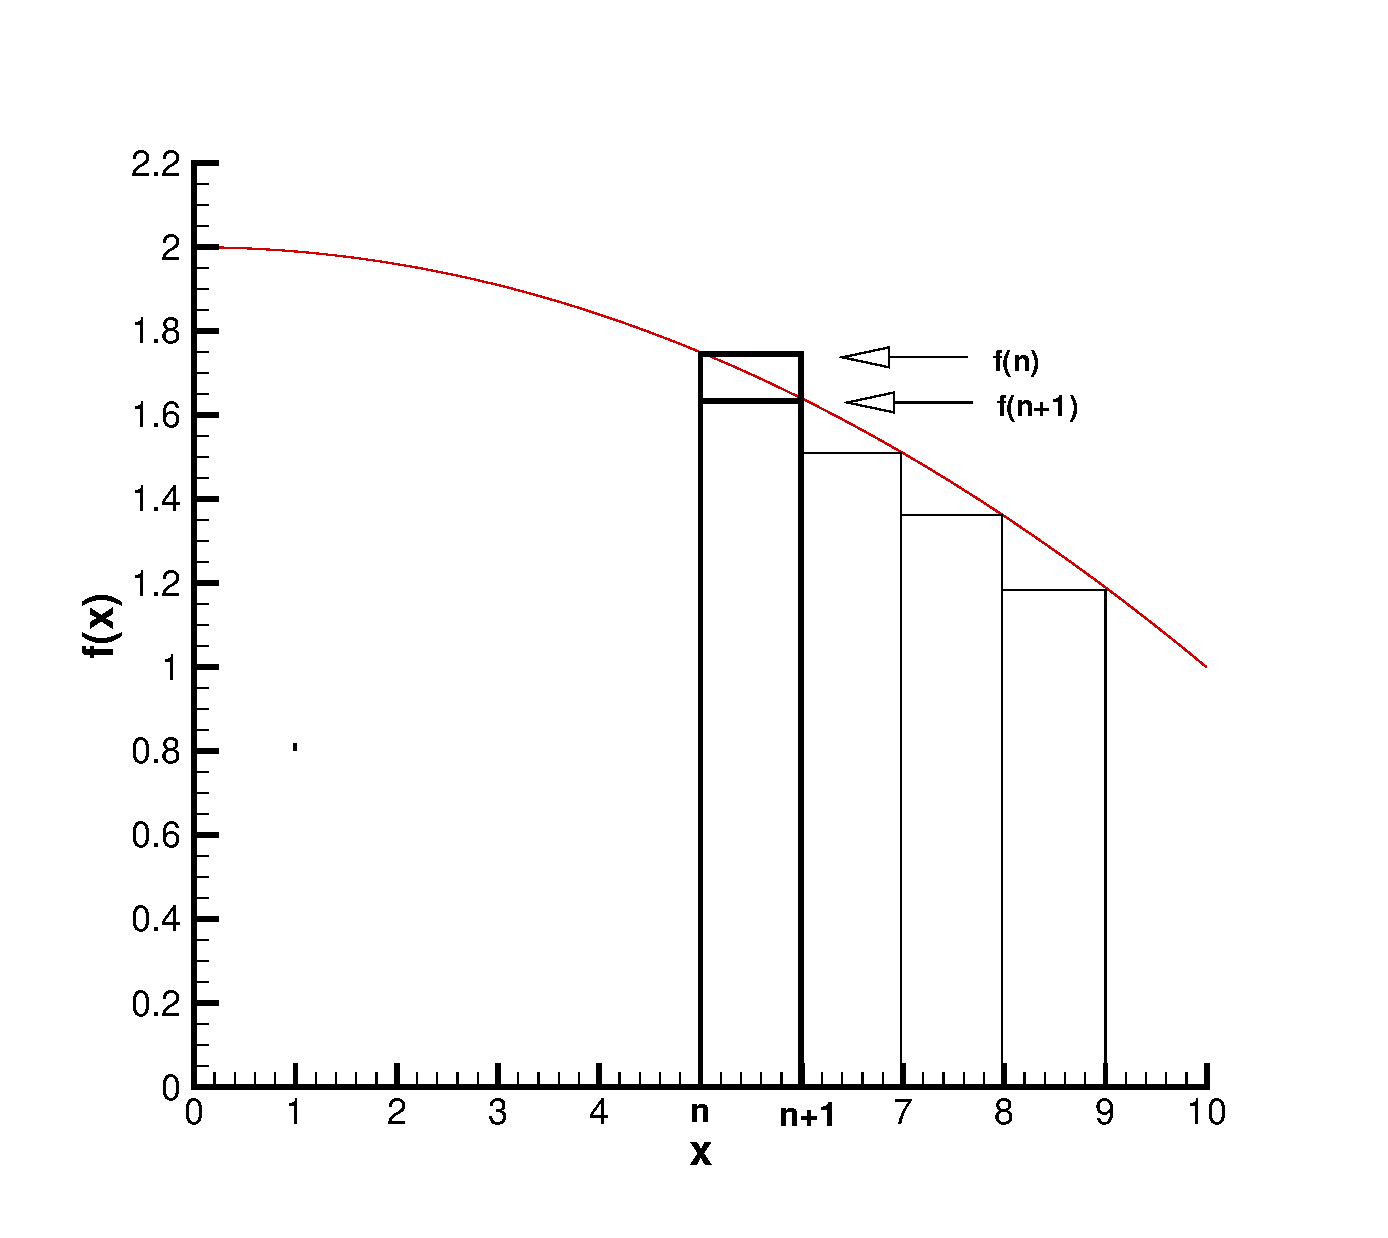
\includegraphics[width= 0.9\textwidth]{./doc/Figures/tecplot/snb}
	%	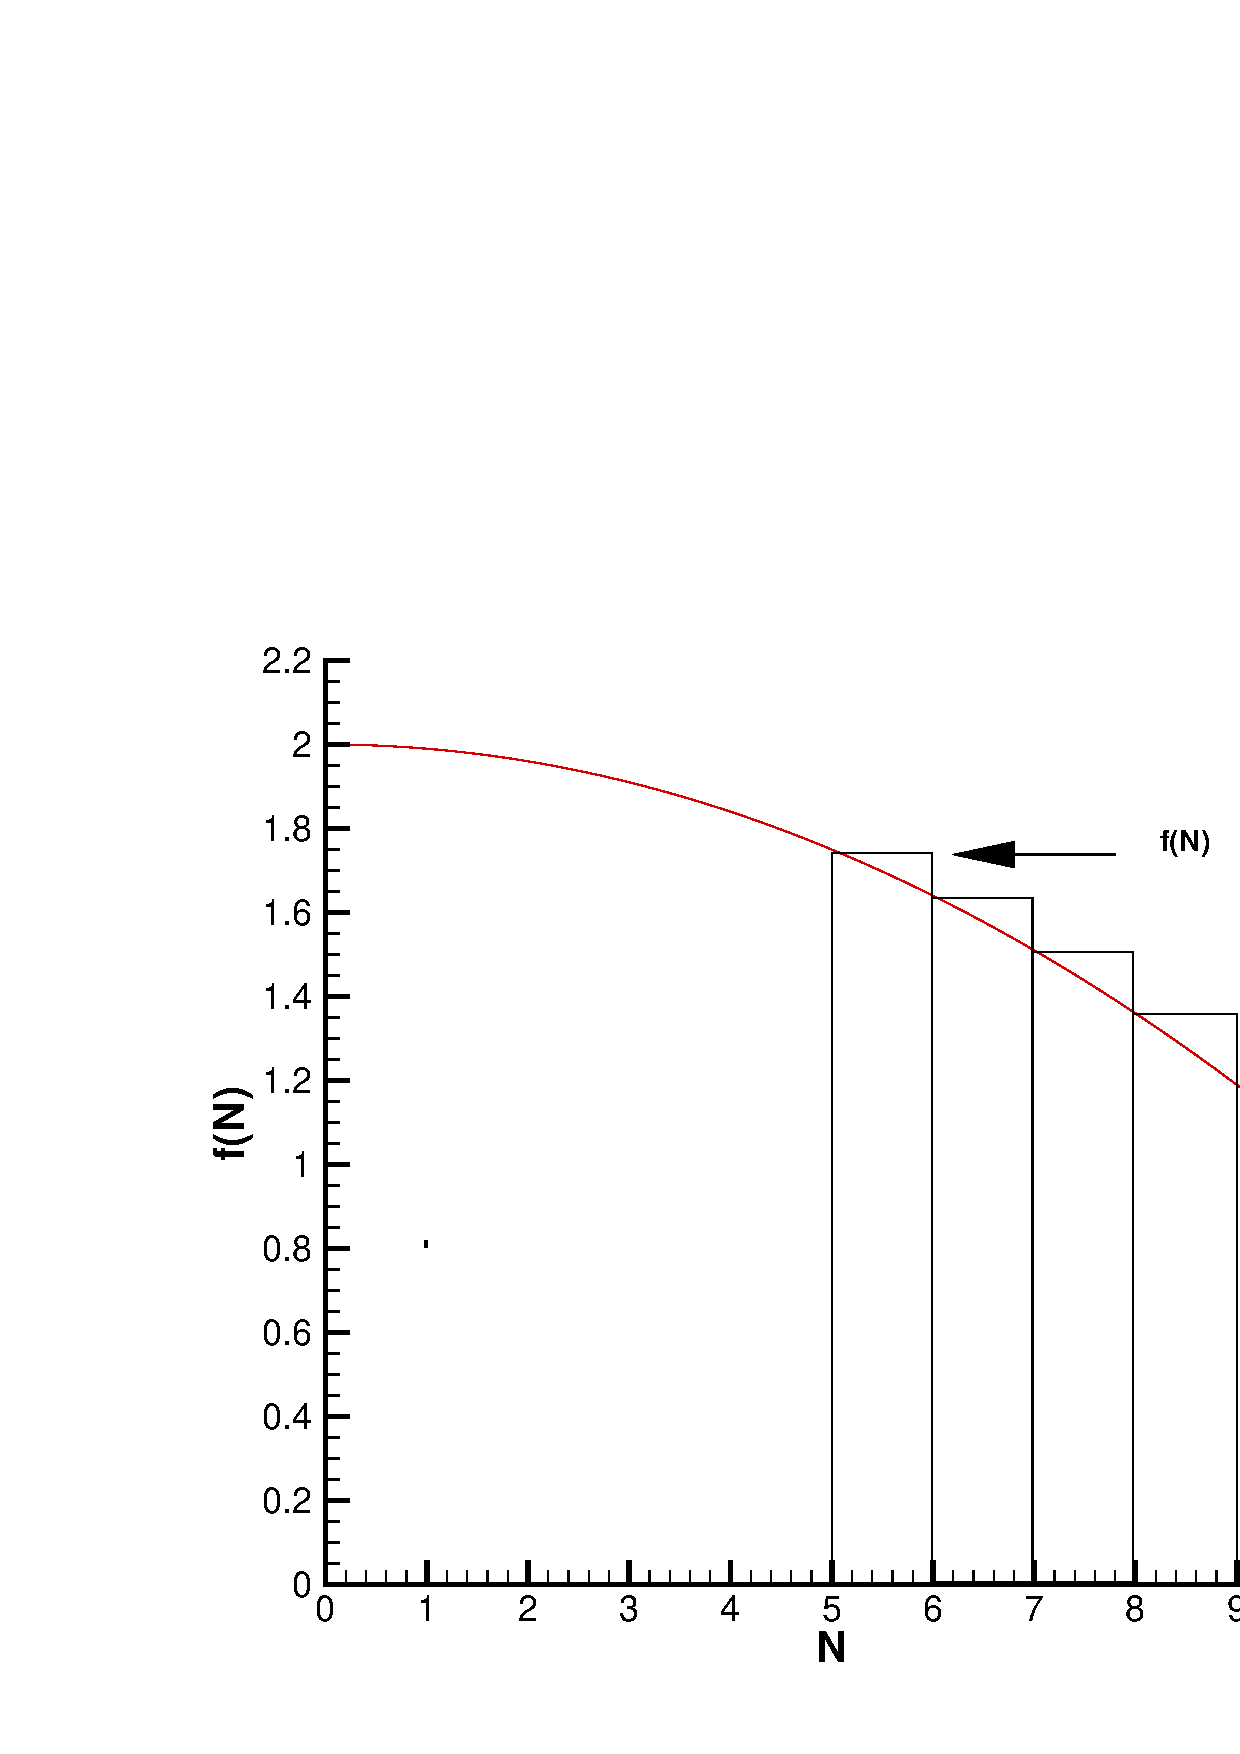
\includegraphics[width= 0.49\textwidth]{Figures/tecplot/sn.pdf}
	\caption{Relation between the integral of $ f:  \mathbb{R} \rightarrow \mathbb{R} $ and a sum of a numerical series with general term $ f 
	: \mathbb{N} \rightarrow \mathbb{R}$.}
	\label{fig:sn}
\end{figure}







    \FloatBarrier
    \subsection{Mathematical support for \texttt{Tail} function}
    
Notice that the function \texttt{Tail} is specially created for good convergence series. It is based on the premise that:
\begin{verbatim} 
    ! Obtain N such as:
    ! integral from i=N+1 to infinity a_i = eps
\end{verbatim}
For a fast convergence sum (the general term tends to 0 quickly), 
the sum is stopped when the truncation error is equal or less than some specific value \texttt{eps}. 
The terms not included in the sum would not appreciably
modify the result. 
For a sum series with a poor convergence the situation is the opposite, stopping the sum when the general term is less than \texttt{eps} 
leaves without adding a huge number of terms whose sum is comparable to \texttt{eps} or even much more higher. Then, the total error committed could be impermissible 
and there resides the difficulties of calculating these series.

Said in other words, the value \texttt{N} that \texttt{Tail} calculates is based on reducing the 
truncation error for good convergence series, not considering that it can be much higher than expected 
if round-off is reached before the truncation error is permissible.

    
    
    
    
    \subsection{First test for bad convergence sum}
For the example we are treating here the bounds of the error are:
\begin{equation}
    \frac{1}{N+1} \le \ S - S_N \ \le \frac{1}{N}
\end{equation} 
Being \texttt{S1} the result of the sum in the computer and using its analytical result,
the total error of the sum is $ \pi^2/6 - \texttt{S1} $.
Then, with the above bounds, the round-off error of the summation gives:

$$
    E_{fl} = E - E_N = \left( \frac{\pi^2}{6} - \texttt{S1} \right) - 1/N
$$
Let's execute now the following example to test this bad convergence sum series: 
\vspace{0.5cm}
\renewcommand{\home}{./Fortran/sources/Foundations/Calculus} 
\listings{\home/Examples/Sum_series.f90}{Summation_n2_examples}
{end subroutine}{Sum_Series.f90} 

First, take a look at the result of the computer if the summation process is stopped according to the 
round-off errors associated to significant digits. Notice that this result is obtained after 94906265 sums.

\begin{verbatim} 
Summation 1/n**2
S =  1.64493405783458   N =  94906265 Error = 9.013651380840315E-009
\end{verbatim}

Now force the computer to calculate the same sum up to 200000000 terms, 
around twice the number of operations than before,
notice that the total error is exactly the same than in the
previous case.

\begin{verbatim} 
S =  1.64493405783458   N = 200000000 Error = 9.013651380840315E-009
\end{verbatim}

If both errors are balanced thanks to the bounds calculated, 
the following results are obtained for the truncation and round-off errors 
(for \texttt{N = 94906265} terms added):

\begin{verbatim} 
Truncation error S =   1.053671197498475E-008
Round--off error   =  -1.523060594144434E-009
\end{verbatim}

Two interesting conclusions are obtained for this example. 
Firstly, 
the round-off error is quite smaller than the error associated to the truncation. 
Secondly,
the error is much higher than the finite number of digits that the computer 
is handling with the sums (in this case around 15 decimal digits). An infinite number of
non-negligible terms are omitted due to a bad convergence rate. 






    \subsection{Second test for bad convergence sum}

Now, the same sum is performed with declarative paradigm, 
calculate the result for a value \texttt{eps = 1e-10} 
and calculate the total error as usual:
\begin{verbatim} 
    real :: S, eps, E
    
    eps = 1e-10
    S = Sigma( a1, 1, eps )
    E = PI**2/6 - S
    
    write(*,*) " Summation 1/n**2 "
    write(*,*) " S = ", S, "Error = ", E    
\end{verbatim}

The following result is obtained, a total error of around \texttt{1e-5} is committed
when the computer is performing sums with terms around \texttt{1e-10}.  

\begin{verbatim} 
Summation 1/n**2
S =    1.64492406689824      Error =   9.999949984074163E-006
\end{verbatim}

A question may appear now; which \texttt{eps} should be introduced to \texttt{Sigma} so the result is calculated until round-off is obtained?
The answer is \texttt{eps = epsilon( S )/2.}, however, some notions of floating-point representation are essential to deepen in this topic.
An extensive discussion regarding the consistency of using \texttt{epsilon( S )} for this example and the generalization for any other sum 
is treated in the section \ref{chap:reals} of Part \ref{PartII} of this book. Also, why dividing it by \texttt{2} is needed becomes clearer. 




 
    \subsection{How can I improve this calculation?}
    
There is a different way of calculating this sum with better accuracy in the computer:
\begin{enumerate}
    \item Using higher precision for the variables, for example quadruple precision for the variables involved. 
    \item Change the algorithm to perform the sum. A non-intuitive way of calculating the sum comes from the fact
    that adding in floating-point arithmetic is not an associative operation. 
\end{enumerate}

Let's perform the same sum backwards, also with double precision and from the lower terms to the higher ones using 1000000000 terms, more than 10 times the maximum terms
used for the forward sum. 

\begin{verbatim} 
Summation 1/n**2
S = 1.64493406584823 N = 1000000000 Error = 1.000000082740371E-009

Truncation error S =   1.000000000000000E-009
Round --off error =   8.274037093680878E-017
\end{verbatim}
 
Surprisingly, just performing the same sums from the lower terms to the higher ones the 
limit of terms found before can be exceeded and the result is ten times more accurate than before. 
As a general rule, when adding numbers with a big difference in magnitude order, 
try to sum first the lower values and then add the result to the higher values. 
Why this improve the result is 
treated in the section \ref{chap:reals} of Part \ref{PartII} of this book.
 
 

\label{numeric_series}








%Dar el resultado de la suma de los 100 primeros términos de las siguientes series: 
%\begin{enumerate}    
%	\item Serie de números naturales.
%	\item Serie de números naturales impares.
%	\item Serie numérica donde el término general de la serie es: $ a_n = 1/n^2 $ desde $ n= 1 $.  
%	\item Serie numérica donde el término general de la serie es $ a_n = 1/ n! $ desde $ n=1$.  % e 
%	\item Serie numérica donde el término general de la serie es
%	$ a_n = (-1)^{n+1}/ (2n-1) $ desde $ n=1$.   
%\end{enumerate}         



%___________________________________________________________________________________________________
\newpage 
\section{Convergence rate}  \label{sec:convergence} 
One of the main focus of the numerical approximation techniques is to attain expansions with high rate of convergence. When dealing with 
numerical series, it is desirable to obtain a precise result by adding the smallest number ot terms to reduce CPU time. 
However, the number of terms to obtain the precise accuracy depends on the convergence rate of the series.
In other words, the behavior of $ a_n $ with $ n \rightarrow \infty $ defines the number of terms to be added. 



In figure \ref{spectral},  $ a_n $ versus $ n $ is represented in log-scale. 
In the same context of discretization techniques, 
if $ a_n = O( 1/n^q) $  for a  given number $ q $, the convergence is algebraic. 
If $ a_n \ll O( 1/n^q) $ for all  q, the convergence is spectral. 
This is shown schematically in figure \ref{spectral}.
\unitlength 0.8mm
\begin{center}
	\begin{figure}[htbp]
		\centering
		\vbox{
			\begin{picture}(120,85)
			
			%   \put(0,0){\framebox(120,85)}
			
			\drawline [200](40,70)(80,50)               
			\drawline [200](40,65)(80,35) 
			\drawline [200](40,60)(80,20)           
			
			\put(30,10){\vector(0,1){70}}
			\put(30,10){\vector(1,0){70}}   
			
			\put(10,78){$\log{|a_{n}|}$}                                        
			\put(90,5){$\log{n}$}
			\put(85,35){Algebraic (line with slope $ q $)}            
			
			\put(38,20){Spectral}    
			
			\qbezier(40,55)(55,40)(60,10)
			
			\qbezier(90,60)(90,40)(70,20)
			
			\put(70,20){\vector(-1,-1){0}}          
			
			
			
			\end{picture} 
			\caption{Convergence of $ a_n $ with $ n $.  Algebraic and spectral  convergence. }
			\label{spectral}
		}
		
	\end{figure}
\end{center}





 
 
 
 
 
   
   
         %___________________________________________________________________________________________________
\chapter{Operations with vectors and matrices}    \label{chap:matrices}


\vspace{-.7cm}
\section{Introduction}

This chapter covers two independent topics through examples. 
In the first place, some essential operations of matrix arithmetic are introduced, 
an operation like the product of two matrices becomes extremely simple 
in programming languages oriented to vector programming. 
In the second place, the concepts of static and dynamic data objects are covered. 
Notice that all the examples are written according to a declarative programming style, 
consider reproducing the same results with an imperative programming style to compare.
    
    \vspace{-.3cm}
    \subsection*{Matrix arithmetic}
    \vspace{-.2cm}

An array programming language or vector language has the possibility 
to operate a whole group of values at once.
The common operations that range over scalar numbers can then be applied to vectors, 
matrices and higher dimension arrays in a closer to maths style. 
Hence, mathematical expressions at the time of programming are simplified.

Languages like Fortran, MATLAB, R or the NumPy extension of Python support array programming.
Matrix arithmetic are built-in in these languages and expressing the mathematical language in a natural way is feasible.

\newpage
The following concepts are covered:
\begin{enumerate}[noitemsep]
    \item Declaring arrays (Fortran): type, rank and dimension.
    \item Initialize arrays: constructors. 
    \item Iterators for arrays, sectors or slices. 
    \item Operations:
    \begin{itemize}
        \item Addition. 
        \item Dot product.
        \item Matrix multiplications. 
        \item Hadamard product. 
        \item Element-wise operations.    
    \end{itemize}
\end{enumerate}  


%Take note of the difference between array programming and array processors. The first makes reference to how the programmer 
%codes the mathematical operations in its program (a big advantage is obtained from this feature for Scientific Computing as mentioned before). 
%The second feature is related to how the processor operates that group of numbers, by performing
%all the operations together under the same instruction given to the processor in a considerably increase of speed.
%Both features suppose an increase of performance for the coding and executing of scientific programs, however, this chapter is 
%oriented to the aspects of the first feature mentioned. 



    \vspace{-.5cm}
    \subsection*{Static/Dynamic data objects}

Each data object declared in a program (variables, constants, pointers, arrays, etc.) are either static or dynamic, 
this means that the memory storage to hold that piece of data is reserved during compilation time or 
during the execution of the program respectively. 

Consider for example the Fortran variable \texttt{real :: A(N, N)} declared at the beginning of a code, 
its memory storage is reserved when the program is compiled and this space is not liberated 
until the program has finished the execution. 

Another option to declare and manage the memory storage of an object involves using dynamic allocation. 
In this case, the storage of the variable is not reserved until the program orders it (which happens during the execution of the code) and can be changed or freed at any moment. 
In Fortran for example, this is done through a code like \texttt{real, allocatable :: Ak(:, :, :)}.

This chapter also includes a review of the main memories that a program uses: Static, Heap and Stack.
All variables, program instructions, constants, etc. are stored in these memories and their use is intimately related 
to the different ways of allocating space in the code.





%___________________________________________________________________________________________________
\newpage 
\section{Declaring, initializing and slicing arrays} 
%Declaration
Consider the vectors $V \in \mathbb{R}^N$, $X\in \mathbb{R}^6$, $Y\in \mathbb{R}^3$ 
and matrices $A \in { \cal{M}}^{N \times N} (\mathbb{R})$, $Z \in { \cal{M}}^{2 \times 3} (\mathbb{R})$
with $N=10$ and let's use arrays to represent them: 
$$
V = \left( v_i =\frac{1}{i^2} \right)^T, \quad A = \left[ a_{ij} = \left( \frac{i}{N} \right)^{j-1} \right], \;\; i = 1 \ldots  N, \;\;  j = 1 \ldots  N   
$$
$$
X = ( 1.3, 2.4, 3, 4.5, 5.3, 7 )^T,  \quad  Y = \left(A_{i j}\right)_{\substack{i = 2 \\  3\leq j\leq 5}}^T, \quad Z =     
\begin{bmatrix}
    1.1 & 2.2 & 3.3\\
    4 & 5.6 & 6.2
\end{bmatrix} 
$$

    \subsection*{Fortran code}

An array, either representing a vector, a matrix or a tensor, is properly \textbf{declared} when it has 
type, rank and dimension (or extent) (see Figure \ref{fig:arrays}). 
The data type has already been treated before, in these examples we are using \texttt{real} vectors and matrices. 
The rank; the number of dimensions in the array, is 1 for column vectors, 2 for matrices and can be higher for higher dimension tensors.
The extent of each particular dimension is its length; the number of elements in that dimension.
\vspace{0.5cm}
\lstfor
\renewcommand{\home}{./Fortran/sources/Foundations/Algebra} 
\listings{\home/Matrix_operations.f90}{subroutine Basic_arrays}{indices of B}{Basic_operations.f90}

\begin{IN}
    Notice that, in Fortran, the \textbf{bounds of a dimension} may start with the index we prefer. 
    By default it stars with index \texttt{1} but it can start in \texttt{0} or whatever index we want. 
    For example the matrix \texttt{B(-2:4,0:1)} starts in \texttt{-2} and ends in \texttt{4} (also included) for the first dimension and 
    \texttt{0} and \texttt{1} (also included) for the second dimension. 
\end{IN}


\newpage
%Initialization
Once declared, the \textbf{initialization} of the arrays is performed with constructors. 
Three ways are commonly used to manually construct an array: 
\vspace{-0.5cm}
\begin{enumerate}[noitemsep]
    \item \textbf{List of values:} \texttt{ [ list ] } where 'list' is a list of values of the same array type separated by commas. 
    \item \textbf{Array slice:} For example \texttt{Y = [ A(2, 3:5) ]} stores the list of values in the second row of \texttt{A} from columns \texttt{3} to \texttt{5}.
    \item \textbf{Implicit loop:} a list of elements is computed from a loop.
\end{enumerate}
In Fortran a list of values can only be used with rank-one arrays so 
the function \texttt{reshape} is needed for higher ranks. 
For example the matrix \texttt{A} in the code is initialized using the \texttt{reshape} function.     
\vspace{0.5cm}
\lstfor
\renewcommand{\home}{./Fortran/sources/Foundations/Algebra} 
\listings{\home/Matrix_operations.f90}{Implicit loop}{By columns}{Basic_operations.f90}   




%sectors, iterators... 
In Fortran the elements of the array are accessed using parenthesis notation and
an index in each dimension can be used as \textbf{iterator}.
This is intimately related to the \textbf{slicing}: referencing a portion of the array by a range of indices.
For example the initialization of \texttt{Y} above use an slice of \texttt{A}.
This can also be extended to a whole dimension using the colon symbol, \texttt{C(:,2)}. 
Furthermore, alternate values can be selected by specifying a lower bound, an upper bound and the jump between values.
Notice that, since Fortran is a column major order language, functions like \texttt{reshape} and slicing treats the data by columns. 
\vspace{0.5cm}
\lstfor
\renewcommand{\home}{./Fortran/sources/Foundations/Algebra} 
\listings{\home/Matrix_operations.f90}{Slices}{columns!}{Basic_operations.f90}  




    \newpage
    \subsection*{Python code}

Let's see the same examples defined above using \texttt{NumPy} arrays.
Notice that now they do not need to be explicitly declared, 
Python automatically does it. 

%Initialization
The \textbf{initialization} of the arrays is performed using the \texttt{array()} function as constructor. 
Three ways are commonly used to manually construct an array: 
\begin{enumerate}[noitemsep]
    \item \textbf{List of values:} \texttt{ [ list ] } or \texttt{ [ [ list ], [ list ] ] } for higher than rank-one arrays,
     where \texttt{list} is a list of values of the same array type separated by commas.
    \item \textbf{Array slicing:} For example \texttt{Y = A(1, 2:5)} stores the list of values in the second row of \texttt{A} from columns \texttt{3} to \texttt{5}.
    \item \textbf{Implicit loop (list comprehension):} a list of elements is computed from a loop.
\end{enumerate}
\vspace{0.5cm} 
\lstpython
\renewcommand{\home}{./Python/sources/Foundations/Algebra} 
\listingsp{\home/Matrix_operations.py}{basic_arrays}{by rows}{data_type.py}



%sectors, iterators...    
In Python, the elements of the array are accessed using bracket notation, 
the array can be \textbf{iterated} using an index in each dimension and 
\textbf{slicing} is also allowed.
Notice that NumPy arrays, contrary to Fortran, are row-major order. 
This means that arrays store the data by rows. 
Similarly to Fortran, the colon symbol iterates in a whole dimension and 
alternate values can be selected by specifying lower and upper bound and the jump between values.
However, the example \texttt{B(-2:4:3,:)} made with Fortran can not be copied because:
\begin{IN}
    In Python, the \textbf{bounds of a dimension} always start with the index \texttt{0} (zero-indexing) and
    stop 1 before the final bound.  
\end{IN}



\newpage
%\begin{figure}[h]
%    \centering
%    \includegraphics[width= 0.8\textwidth]{./doc/Figures/FixedFloat3.png}
%    \caption{Representation of number 20.25 with fixed-point format using only 1 byte (8 bits).}
%    \label{fig:FixedFloat2}
%\end{figure}
\FloatBarrier
\begin{figure}[b]
    \centering
    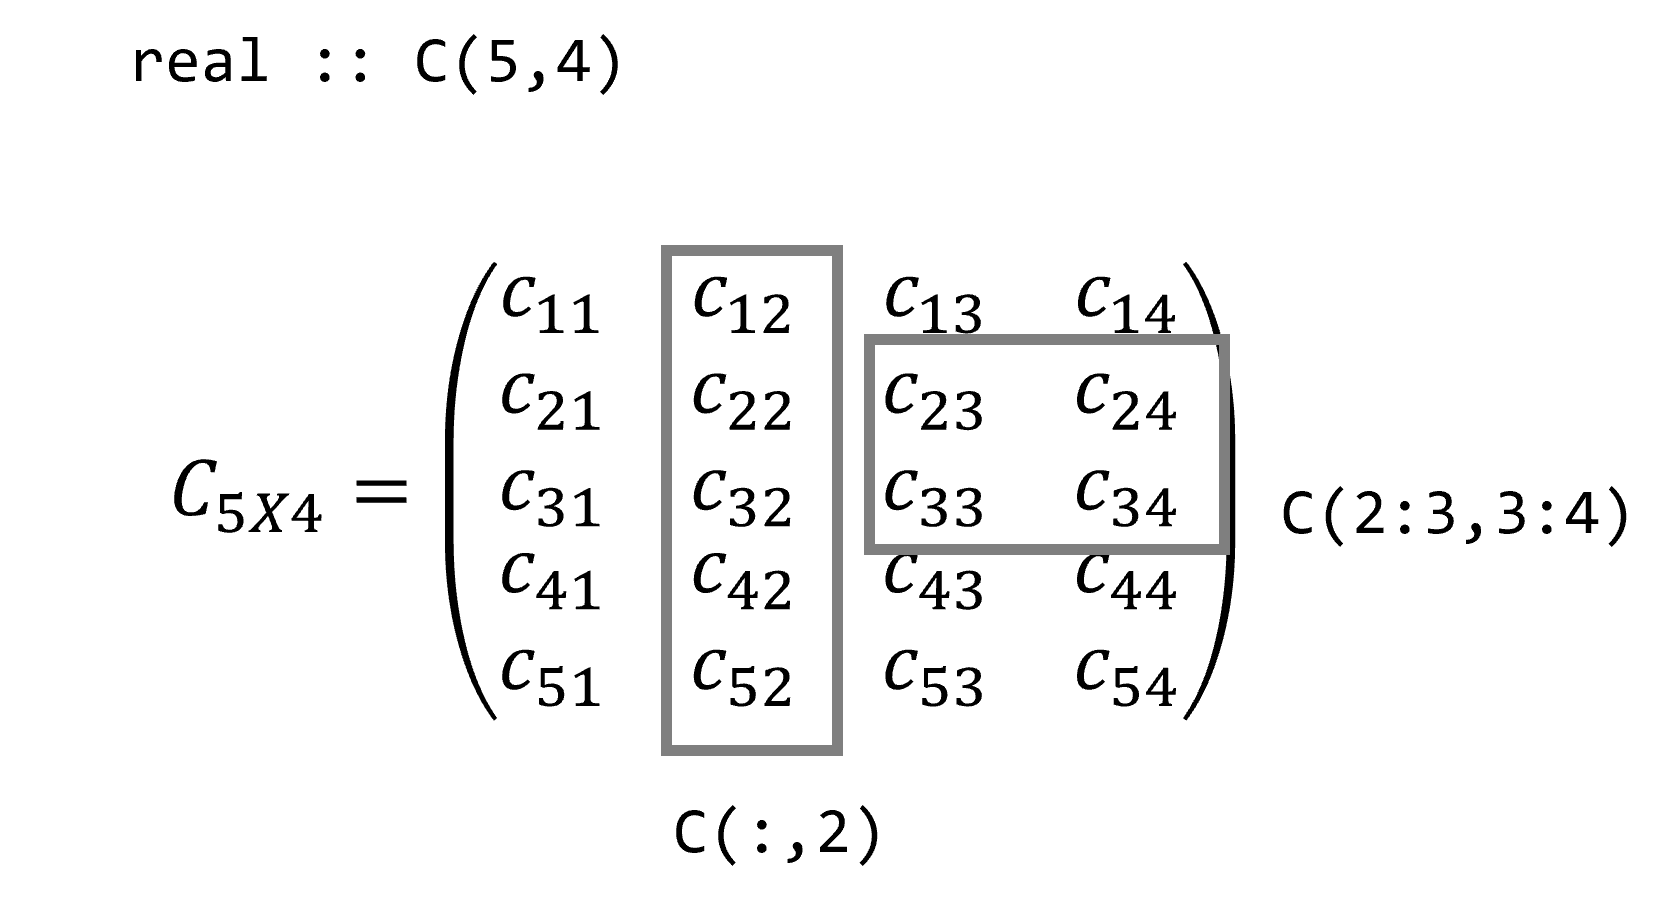
\includegraphics[width = .8\textwidth]{./doc/Figures/Array1.png}  \\
    \begin{center}
        Rank = 2 \\
        Extent = (5,4) \\
        Size = 20 \\
        Bounds = (1:5, 1:4) \\
        %Shape = (5, 4)
    \end{center}
\end{figure}

\begin{figure}[b]
    \centering
    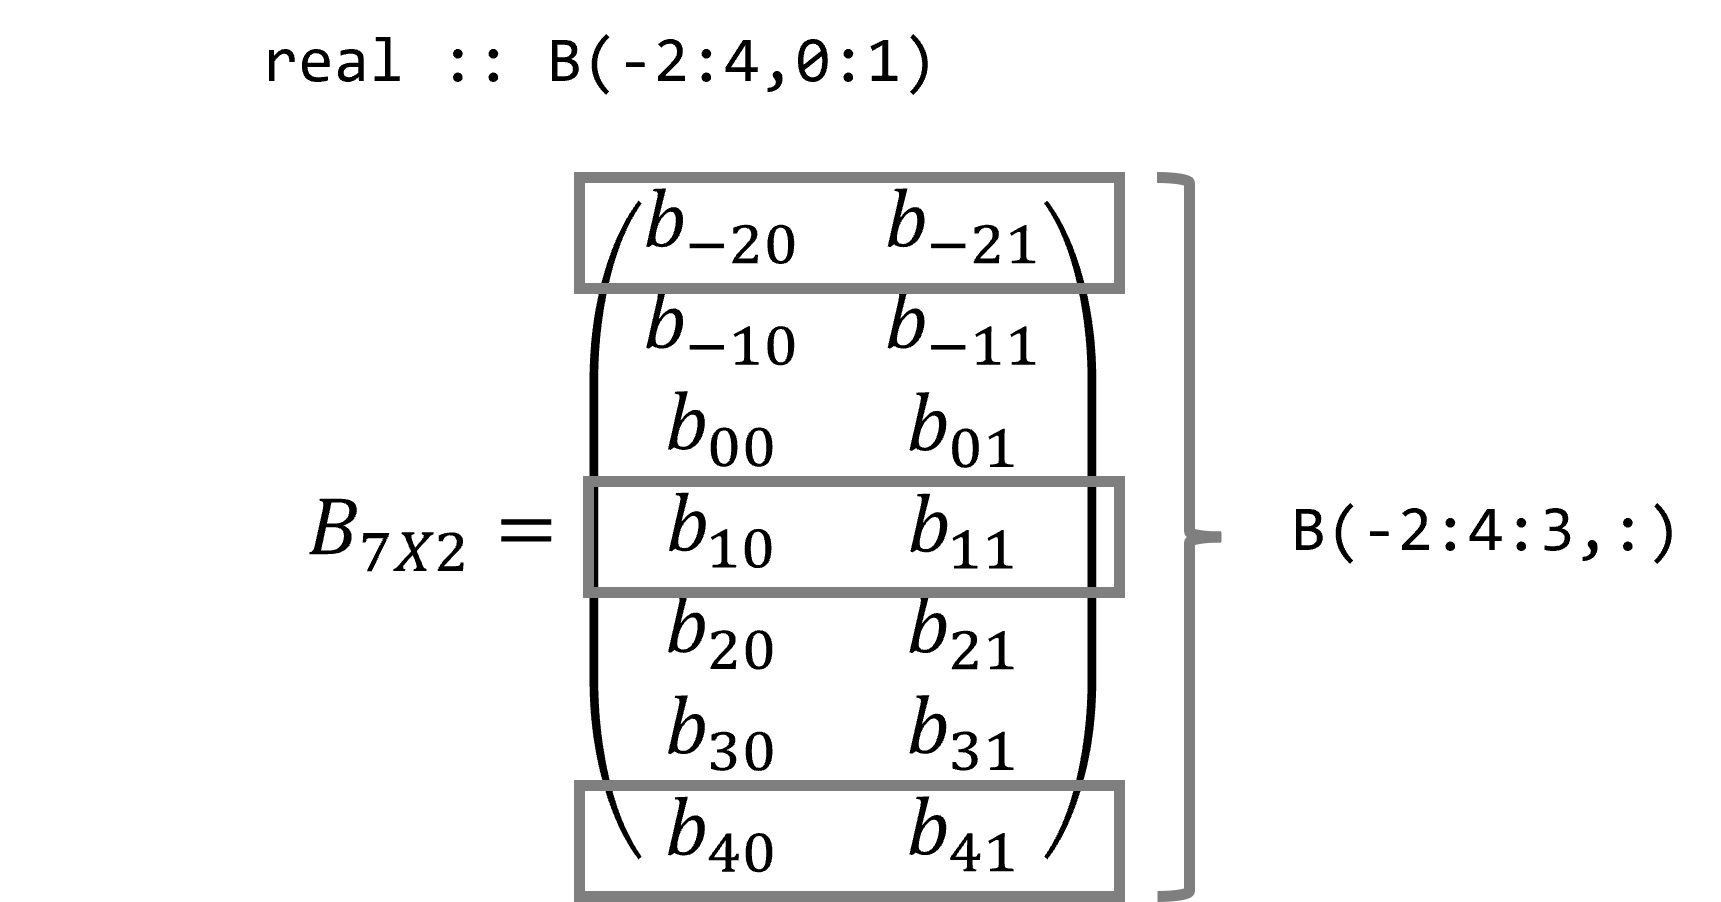
\includegraphics[width = .8\textwidth]{./doc/Figures/Array3.png}  \\
    \begin{center}
        Rank = 2 \\
        Extent = (7,2) \\
        Size = 14 \\
        Bounds = (-2:4, 0:1) \\
        %Shape = (7, 2)
    \end{center}
\caption{Example arrays with their main properties.}   \label{fig:arrays}
\end{figure}

%\begin{figure}
%    \begin{subfigure}[b]{0.5\textwidth}
%        \centering
%        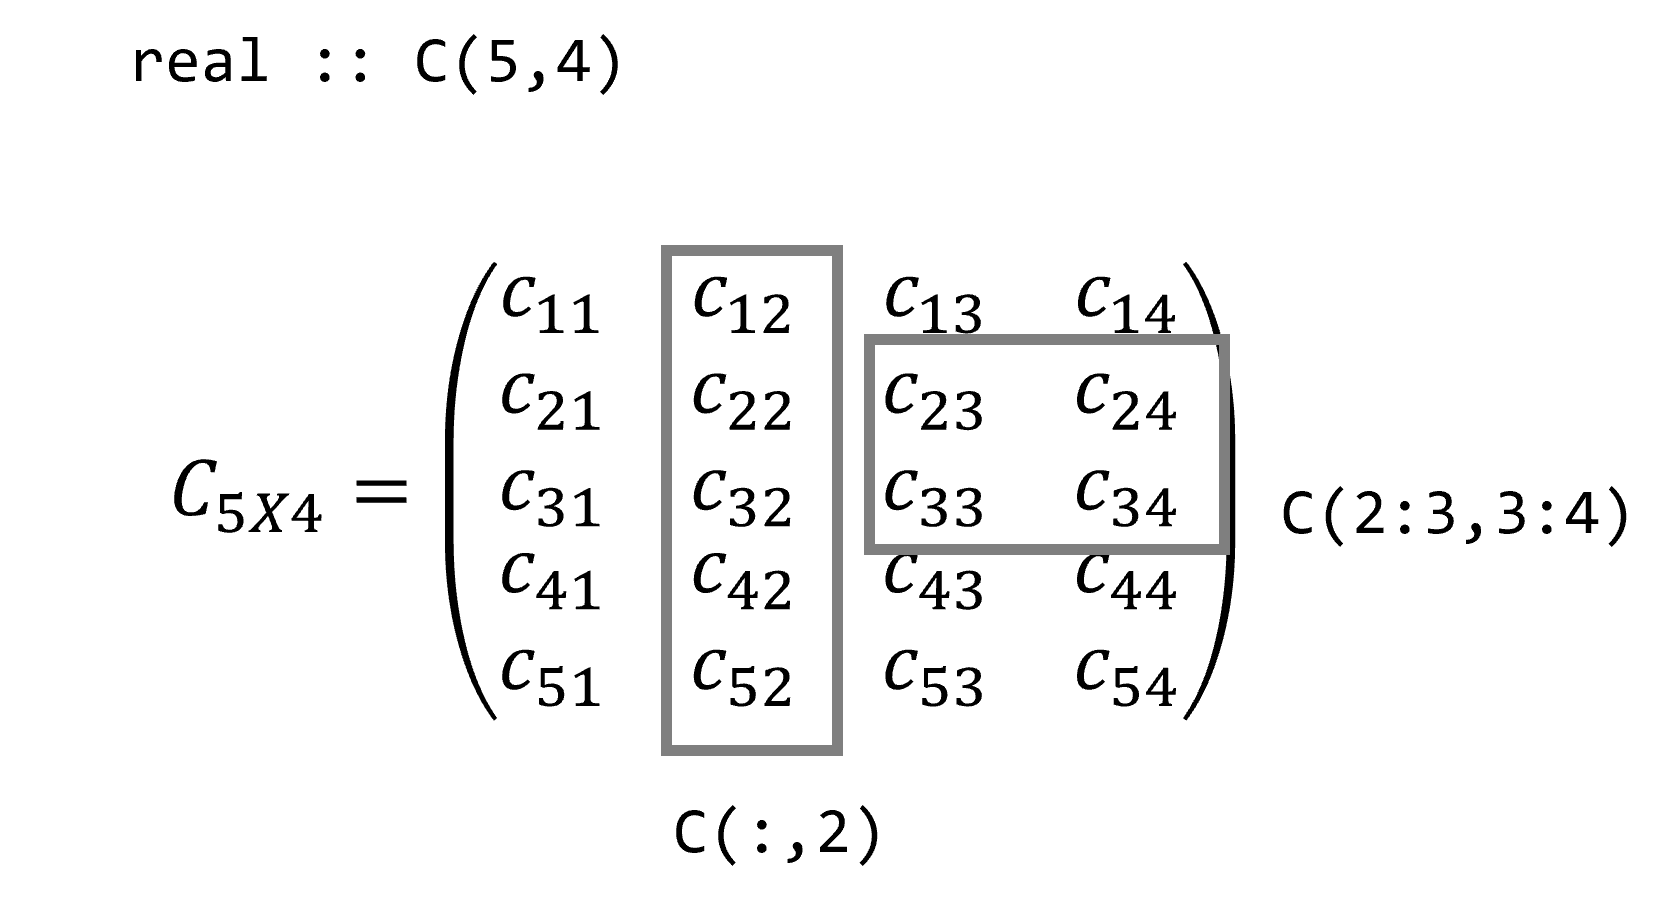
\includegraphics[width = \textwidth]{./doc/Figures/Array1.png}  \\
%        \begin{center}
%            Rank = 2 \\
%            Extent = (5,4) \\
%            Size = 20 \\
%            Bounds = (1:5, 1:4) \\
%            %Shape = (5, 4)
%        \end{center}
%    \end{subfigure}
%    \hspace{\fill}
%    \begin{subfigure}[b]{0.5\textwidth}
%        \centering
%        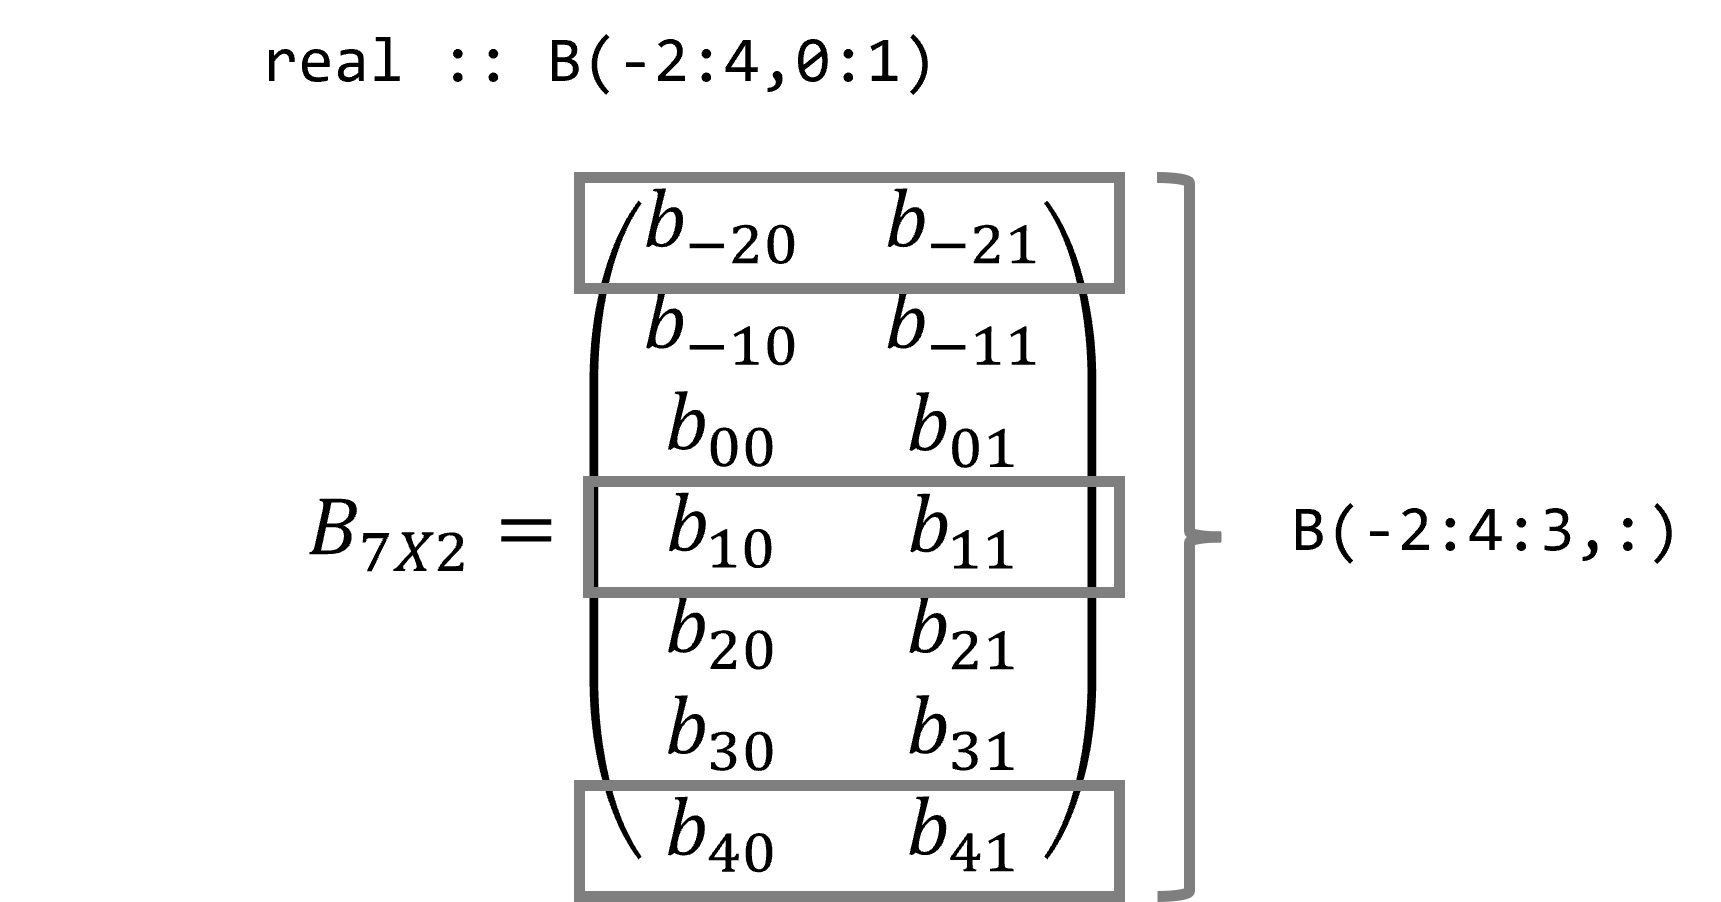
\includegraphics[width = \textwidth]{./doc/Figures/Array3.png}  \\
%        \begin{center}
%            Rank = 2 \\
%            Extent = (7,2) \\
%            Size = 14 \\
%            Bounds = (-2:4, 0:1) \\
%            %Shape = (7, 2)
%        \end{center}
%    \end{subfigure}
%    \caption{Example arrays with their main properties.}   \label{fig:arrays}
%\end{figure}


\FloatBarrier


%___________________________________________________________________________________________________
\newpage 
\section{Static size vectors and matrices} 

Consider the same vectors $V, W \in \mathbb{R}^N$ and matrices $A, B \in { \cal{M}}_{N \times N} (\mathbb{R})$ used in the previous section (with $N=10$): 
$$
V = \left[ v_i =\frac{1}{i^2}, \ \ i = 1 \ldots  N \right],
$$
$$
W = \left[ w_i = \frac{(-1)^{i+1}}{2i+1}, \ \ i = 1 \ldots  N \right],
$$
$$
A = \left[ a_{ij} = \left( \frac{i}{N} \right)^{j-1}, \ \ i = 1 \ldots  N, \ \ j = 1 \ldots  N \right],
$$
$$
B = A^T
$$
and let's compute the following matrix operations:
$$
1.\;\sum_{i=1}^N v_i  \qquad \qquad 2.\;\sum_{i,j=1}^N a_{ij}   \qquad \qquad   3.\;\sum_{v_i>0} v_i   \qquad \qquad 4.\;\sum_{\scriptstyle i,j=1 \atop \scriptstyle a_{ij} > 0.1}^N a_{ij}   
$$
$$
5.\; V\cdot W^T    \quad \quad      6.\; V\cdot [a_{ij}]_{\scriptstyle 1\leq i\leq N \atop \scriptstyle j = N}    \quad  \quad  7.\; AV     \quad \quad   8.\;\sum_{i,j=1}^N [A^2]_{ij}   \quad \quad    9.\; B = A^T
$$
$$
10.\;\max_{1\leq i,j\leq N} \{ a_{ij} \}       \qquad \qquad     11.\;\arg\max_{1\leq i,j\leq N} \{ a_{ij} \}   
$$

Apart from matrix operations, programming languages also support element-wise operations,
those where the result is an equal shaped array with the results of applying the operation to each/corresponding elements.
Let's compute for example the addition of two matrices, the Hadamard product (where corresponding elements are multiplied)
or some elemental operations that can also be applied to matrices apart from numbers: cosine or square root. 
Notice that, where needed $i,j = 1\ldots N$ with $N=10$:
$$
1.\;\Tr(A + B)  \quad \quad 2.\;\Tr(A\odot B)  \quad \quad   3.\;\Tr( \left[ cos( a_{ij} )\right] )   \quad \quad 4.\;\Tr( \left[ \sqrt{a_{ij}} \right] )
$$

Since the sizes of these arrays are known at compile-time, the memory storage can be declared statically. 
The main properties of a static allocation are:
\begin{enumerate}
    \item The memory address and the size are assigned during the compilation of the code in the executable image of the program.
    \item These address and size can not be changed during execution.
    \item Once the program finishes the execution the space is freed.
    \item It is a simple and quick allocation process.
\end{enumerate}



        \newpage
        \subsection*{Fortran code}
The following code computes these operations using Fortran. 
Notice that these examples are limited to numeric arrays: integers, reals or complex,
however, arrays can be constructed with a different data type. 
Furthermore, new operations could be defined for other data types. 
    
Consult the specifications of the following matrix operations to become familiarized with the purpose, inputs and arguments.
Notice that the rank and dimension of the arguments must agree with the mathematical definitions of the operations.
As a quick reference: 
\begin{itemize}[noitemsep]
    \item \texttt{sum} adds all elements of an array: across one dimension, all the dimensions 
    or only the elements that accomplish with some condition (e.g. $v_i > 0$).
    \item \texttt{dot\_product} calculates the scalar product of two vectors.
    \item \texttt{matmul} computes a matrix multiplication. 
    \item \texttt{transpose} calculates the transpose of a matrix or vector. 
    \item \texttt{maxval} and \texttt{maxloc} return the maximum value from all the elements of an array and its position respectively.
    It can compute the result across one dimension, the whole array or only for those values that accomplish with a specified condition.
\end{itemize}

\lstfor
\renewcommand{\home}{./Fortran/sources/Foundations/Algebra} 
\listings{\home/Matrix_operations.f90}{subroutine Matrix_operation_examples}
      {end subroutine}{Matrix_operations.f90}

Let's remark some interesting notes of this code. 
First of all, \texttt{N} (which declares the size of the arrays) is declared as a named constant thanks to the \texttt{parameter} attribute. 
Hence, its value is fixed during the whole execution and a try to change it returns a compilation error. 

Secondly, to initialize both \texttt{V} and \texttt{W} their definition is written by means of an implicit loop (declared with parentheses). 
To define the matrix \texttt{A} two implicit loops are used: 
the nested loop \texttt{i} iterates in the rows while 
\texttt{j} jumps from one column to the next one. 
Both loops define a $N\cdot N$ rank-one vector that needs to be reshaped to a ${\mathbb{R}}^{N\times N}$ matrix. 
The function \texttt{reshape} organizes the components of the vector into columns. 

Finally, notice how an implicit loop with a colon symbol \texttt{:} is also used
in the scalar product of the vector \texttt{V} with the $N$-th column of \texttt{A}. 
The implicit loop in \texttt{A} iterates in the \texttt{N} elements of the column. 
Another example would be how the matrix \texttt{B} is written in the screen,
it uses two loops (one explicit and one implicit) so each row of the matrix is represented element by element.
Compare this way with the output of the line \texttt{write(*,*) B} where all the elements are represented by columns and not by rows. 
This is due to the fact multidimensional arrays are stored in a linear storage and Fortran,
which is a \textit{column-major order} language, organizes the consecutive elements of a column one next to each other.

The following code computes the proposed element-wise operations using Fortran.
\vspace{0.5cm} 
\lstfor 
\listings{\home/Matrix_operations.f90}{subroutine ElementWise_operation_examples}
{end subroutine}{Matrix_operations.f90}




         \newpage 
        \subsection*{Python code}
The same function can be written almost identically with Python. 
Notice from the following code how all vectors and matrices are constructed by using similar implicit loops. 
In addition, the same intrinsic functions are implemented so the use of mathematical notation when programming becomes natural.
Some particularities in this examples would be the indentation or the use of implicit typing. 
%\vspace{0.5cm} 
\renewcommand{\home}{./Python/sources/Foundations/Algebra} 
\lstpython
\listingsp{\home/Matrix_operations.py}{def Matrix_operation_examples}
      {WARNING}{Matrix_operations.py} 

The following code computes the proposed element-wise operations using Python.
\vspace{-.5cm}
\lstpython
\listingsp{\home/Matrix_operations.py}{def ElementWise_operation_examples}
{END}{Matrix_operations.py}





%_______________________________________________________________________________________________
\newpage  
\section{Dynamic allocation of vectors and matrices} 

Now let's use the square Vandermonde matrix  of $M\times M$:
$$
A_M =  \left[ a_{ M_{ij} } = \left( \frac{i}{M} \right)^{j-1}, \ \ i = 0, \ldots M-1, \ \  j=0, \ldots M-1 \right],  
$$
to compute the following operations:
$$ 
S = \sum_{M=1} ^{10} \Tr(A_M)  \qquad
S = \sum_{M=1} ^{5} \Tr(A_M^2) \qquad
S = \Tr \left( \sum_{k=0} ^{5} A_M^k  \right)  \qquad  M=8 
$$

Imagine now that the size of the matrix involved in your code is not known at compile-time, maybe it comes from 
an user input, 
an external file or 
it is the result of a previous operation. 
In this case, dynamic data objects are used so its memory storage (address, size, etc.) is allocated or modified during the execution of the program.
In Fortran for example the essential statements used to manage the memory are 
\texttt{allocate} and \texttt{deallocate} while the attribute for the data object is \texttt{allocatable}. 
The main properties of dynamic data objects are:

\begin{enumerate}
    \item The program decides how much memory reserve for a data objects so it can accommodate any size with no need of re-compiling the code.
    \item Modifications for the memory size are allowed. 
    \item It becomes the programmer responsibility to liberate the memory reserved for non-used arrays in order not to run out-of-memory.
    \item It is generally slower than static allocation. 
\end{enumerate}

The following examples, whether coded in Fortran or Python, are based on the following functions: 
\begin{itemize}[noitemsep]
    \item \texttt{Vandermonde( M )} which computes the Vandermonde matrix of a given dimension \texttt{M},
    \item \texttt{trace( A )} to compute the trace of a matrix and
    \item \texttt{power( a, k )}, a recursive function to obtain the $k$-th power of a matrix.
\end{itemize}
Once each function is coded, more general operations are easy to implement. 
In addition, remember that each abstraction can now be used in any program where this algebra is needed from now on. 




    \newpage 
    \subsection*{Fortran code}

The subroutine \texttt{Matrices\_allocation()} computes the mentioned operations in Fortran:
\lstfor
\renewcommand{\home}{./Fortran/sources/Foundations/Algebra} 
\listings{\home/Dynamic_allocation.f90}{subroutine Matrices_allocation}
{end subroutine}{Dynamic_allocation.f90}

Let's take a deeper look into the program. 
Notice that the 3-rank object \texttt{Ak} is declared with the attribute \texttt{allocatable} and colons \texttt{:} instead of the dimension specifications. 
Later, when the dimensions are known, the \texttt{allocate} function is used to reserve the appropriate memory for the variable.

For the first operation, the expression \texttt{trace( Vandermonde(M) )} is coded inside an implicit loop from 1 to 10. 
These results are constructed in a vector (using squared brackets) and 
\texttt{sum} performs the summation of the components of that vector. 
In addition, notice the use of few variables thanks to a declarative style. 
In an imperative style each Vandermonde matrix would be explicitly stored in a variable \texttt{AM(M,M)} and
their traces in a real vector variable used as an input for \texttt{sum} function. 
%Do not think that these objects are not used now, the compiler still needs them. 
%However, it automatically reserves memory, stores the intermediate results, returns only the single result needed \texttt{S} and, 
%when the calculation is finished, frees all that temporary memory used in an efficient way. 

The second operation is similar with the exception that now the trace is calculated on the product of two matrices. 
%Fortran, like any common scientific language already has implemented the product between two matrices of reals. 
A vector programming style has advantages to code algebra expressions as we know, 
but it also has a better performance when computing multiple operations if vector processors are used.
This is due to an increase in efficiency when the same operation is performed over a bunch of numbers. 

\newpage
For the third operation the variable \texttt{Ak} is dynamically allocated with bounds 0 to 5 in the third dimension. 
While normally the indices of any array starts in 1, the programmer may decide to modify it 
so the index automatically responds to a mathematical sense.
In this case, starting in 0, we allow \texttt{Ak(:,:,k)} to be a reference to the $k$-th power.
%with no need of remembering in which index starts and how many powers are we calculating. 
%If the needed powers of Vandermonde would only have been 4, 5 and 6, we could have allocated the matrix like: \texttt{allocate( Ak(8, 8, 4:6) )}. 
Finally, notice the complete array assignation performed with \texttt{Ak}. 
Once it is properly allocated, writing \texttt{Ak(:,:,k) =} is enough to store the result since it is previously known that the result is an $8\times8$ matrix. 
%Also, it is mandatory to specify to the function \texttt{sum} that the summation is only performed in the third dimension of \texttt{Ak} so it is adding one matrix to the next one. 

\vspace{0.5cm}
\listings{\home/Dynamic_allocation.f90}{function trace}
{end function}{Dynamic_allocation.f90}

\listings{\home/Dynamic_allocation.f90}{function power}
{end function}{Dynamic_allocation.f90}
For the functions \texttt{power( A, k )} and \texttt{trace( A )} two concepts should be extracted. 
Firstly, both must be used only with square matrices, where both mathematical operations are defined. 
Secondly, the concept of recursion is used to calculate the $k$-th power of a matrix. 
Essentially, the $k$-th power of a matrix is the multiplication of that matrix with his $k-1$-th power. 
A \texttt{recursive} statement is used in the declaration so the compiler knows that this function can call to itself to compute smaller instances of itself.
In this example it is going to compute the $k-1$-th power when trying to compute the $k$-th, 
the $k-2$-th power when trying to compute the $k-1$-th and so on until the identity matrix is reached (power 0). 



    \newpage
    \subsection*{Python code}
The same functions are written with Python in a similar style:
the use of implicit loops to construct arrays, 
the use of similar intrinsic functions or 
the need to define those functions not built-in in the language.
In this sense, the function \texttt{trace} belongs to the \texttt{numpy} library so there is no need to code it.

\vspace{0.5cm}
\lstpython
\renewcommand{\home}{./Python/sources/Foundations/Algebra} 
\listingsp{\home/Dynamic_allocation.py}{def Matrices_allocation}
{return}{Dynamic_allocation.py}

\listingsp{\home/Dynamic_allocation.py}{def power}
{matmul}{Dynamic_allocation.py}



\newpage
\section{Memories: Static, Heap, Stack}
During the execution of a program certain amount of memory is needed to store data objects and the source code. 
The compiler, the linker and the operating system of the machine decides where each piece of data is stored. 
Three regions of memory are distinguished: static, heap and stack (see Figure \ref{fig:Memories}). 
Each one is related to one type of allocation, static kind of allocation for the static region and dynamic in nature for the other two.

Static and dynamic allocations have been already used in this chapter. 
The third type of allocation is the stack (or automatic) allocation. 
The compiler is constantly using it, 
for example to store temporary arrays inside subroutines/functions 
or to store temporary arrays from array expressions.

Let's first review how each memory region works:
\begin{itemize}
    \item \textbf{Static:} it is usually located in the low end of the memory reserved for the application. 
    The compiler creates a list of objects to be allocated during the compilation and gives them a fixed address.
       
    \item \textbf{Heap:} the program requests a specific amount of memory to the system during run-time.
    If there is available space, the system responds with the starting address where storing the data. 
    When that space is no longer needed, the program can ask the system to free up the memory so it is available for the next time.
    For some purposes the programmer can manage the allocation and deallocation of space, for the rest, the compiler automatically manages it. 
   
    \item \textbf{Stack:} it is composed by a limited amount of memory and a pointer that marks how full it is. 
    With this pointer, the routines know where to store local variables at a specific moment. 
    This memory space is filled from the top to the bottom: 
    if a function needs temporary storage, let's say \texttt{functionA}, then it fills in the Stack starting in the pointer.
    Hence, the pointer is decremented and the stack space is reduced. 
    If \texttt{functionA} calls a nested \texttt{functionB} then the new local variables are stored below the variables of \texttt{functionA} and the pointer is decremented again. 
    Once \texttt{functionB} finishes its execution, the pointer is incremented and the memory is freed so that space is available for the next routine. 
    This structure is called ``Last-In, First-Out'' (LIFO).  
\end{itemize}

Notice that the whole program can access the objects stored in the \textbf{static} at any time in a quick way.
However, it requires knowing the amount of memory needed at compile-time.
Comparing \textbf{heap} and \textbf{stack}, the amount of heap space is usually bigger than the stack, but it is not unlimited. 
Hence, if no heap deallocation is performed, a memory leak can happen (space still reserved with no useful data).
Concepts like virtual memory and swap play an important role then. 
The use of stack is an efficient and fast process (usually faster than the heap).
In addition, this space is automatically freed when a routine ends its execution. 
Although this allocation is performed by the machine,
the programmer usually has some control over it. 
For example in Fortran, some variables can be declared as \texttt{AUTOMATIC} inside subprograms so they are necessarily saved in the stack. 
However, in Windows, the linker limits the amount of stack and the programmer must be careful about allocating more space than is available in order to avoid stack overflow.   

In the following examples the problem of Stack overflow is simulated.
It usually happens in two situations; large array variables and extremely deep (or infinite) recursion. 


 
    \subsection*{Fortran code}

%Primer ejemplo de stack overflow
In the following example let's allocate a $400\times400\times400$ 4-bytes reals array first in the heap (\texttt{R}) and 
then in the Stack through an automatic array (\texttt{S}) using the function \texttt{StackOverflow\_size( n )}. 
Notice that there is not errors in compile-time since there is enough space in the heap, 
however, during the execution a \texttt{Program Exception - stack overflow} appears.
\vspace{0.5cm}
\lstfor
\renewcommand{\home}{./Fortran/sources/Foundations/Algebra} 
\listings{\home/Stack_Overflow.f90}{subroutine StackOverflow_LargeArrays}
{end subroutine}{Stack_Overflow.f90}

\listings{\home/Stack_Overflow.f90}{function StackOverflow_size}
{end function}{Stack_Overflow.f90}

\newpage
Some strategies can be used to avoid this error:
\begin{enumerate}
    \item Try to reduce the abuse of stack: allocate automatic arrays that usually goes to stack so they are located in heap and automatically deallocated at the end of the routine. 
    \item Increase the size of the stack: in Visual Studio for example a linker option can be specified, \texttt{/STACK:100000000} where the number indicates the size in bytes.
    \item Change the default location for automatic arrays and temporary arrays: they can be automatically located in the heap by using the compiler option \texttt{/heap-arrays}. 
    By specifying a kilobytes size, i.e \texttt{/heap-arrays100}, only larger arrays are allocated in the heap. 
    Use the compiler option \texttt{/heap-arrays0} to apply the behaviour to all arrays.   
\end{enumerate}
As an exercise try to execute this example changing the default location for automatic arrays and temporary arrays. 
In Visual Studio it can be done in the project properties by clicking on \textit{Configuration Properties/Fortran/Command Line} and adding \texttt{/heap-arrays0}.

%Segundo ejemplo de stack overflow
In the following example the end condition of a recursive procedure is incorrectly defined.
The code shows the same function \texttt{power} used in the Dynamic allocation examples, 
but now the end condition (\texttt{if (k >= 10) then}) is incorrectly implemented (\texttt{wrong\_power}). 
Notice that computing a power smaller than \texttt{k = 10} will result in an endless recursion.
This could also happen if, by mistake, the recursion is defined with increasing powers instead of decreasing 
even when the end condition is properly defined. 

Sometimes Fortran could stop working before breaking by a Stack Overflow error.
In this case, since the recursion is performed with a big \texttt{matrix} in each call ($100\times 100$),
the Stack Overflow error breaks the execution. 
Notice that both examples are commented in the project so as not to break the flow.
\vspace{0.5cm}
\lstfor
\renewcommand{\home}{./Fortran/sources/Foundations/Algebra} 
\listings{\home/Stack_Overflow.f90}{StackOverflow_InfiniteRecursion}
{end subroutine}{Stack_Overflow.f90}

\newpage
\listings{\home/Stack_Overflow.f90}{recursive function wrong_power}
{end function}{Stack_Overflow.f90}

    %\subsection*{Python code}
%The same issues appear with Python.
%the use of implicit loops to construct arrays, 
%the use of similar intrinsic functions or 
%the need to define those functions not built-in in the language.
%In this sense, the function \texttt{trace} belongs to the \texttt{numpy} library so there is no need to code it.
%  
%Primer ejemplo de stack overflow


%Segundo ejemplo de stack overflow




\begin{figure}[h]
    \centering
    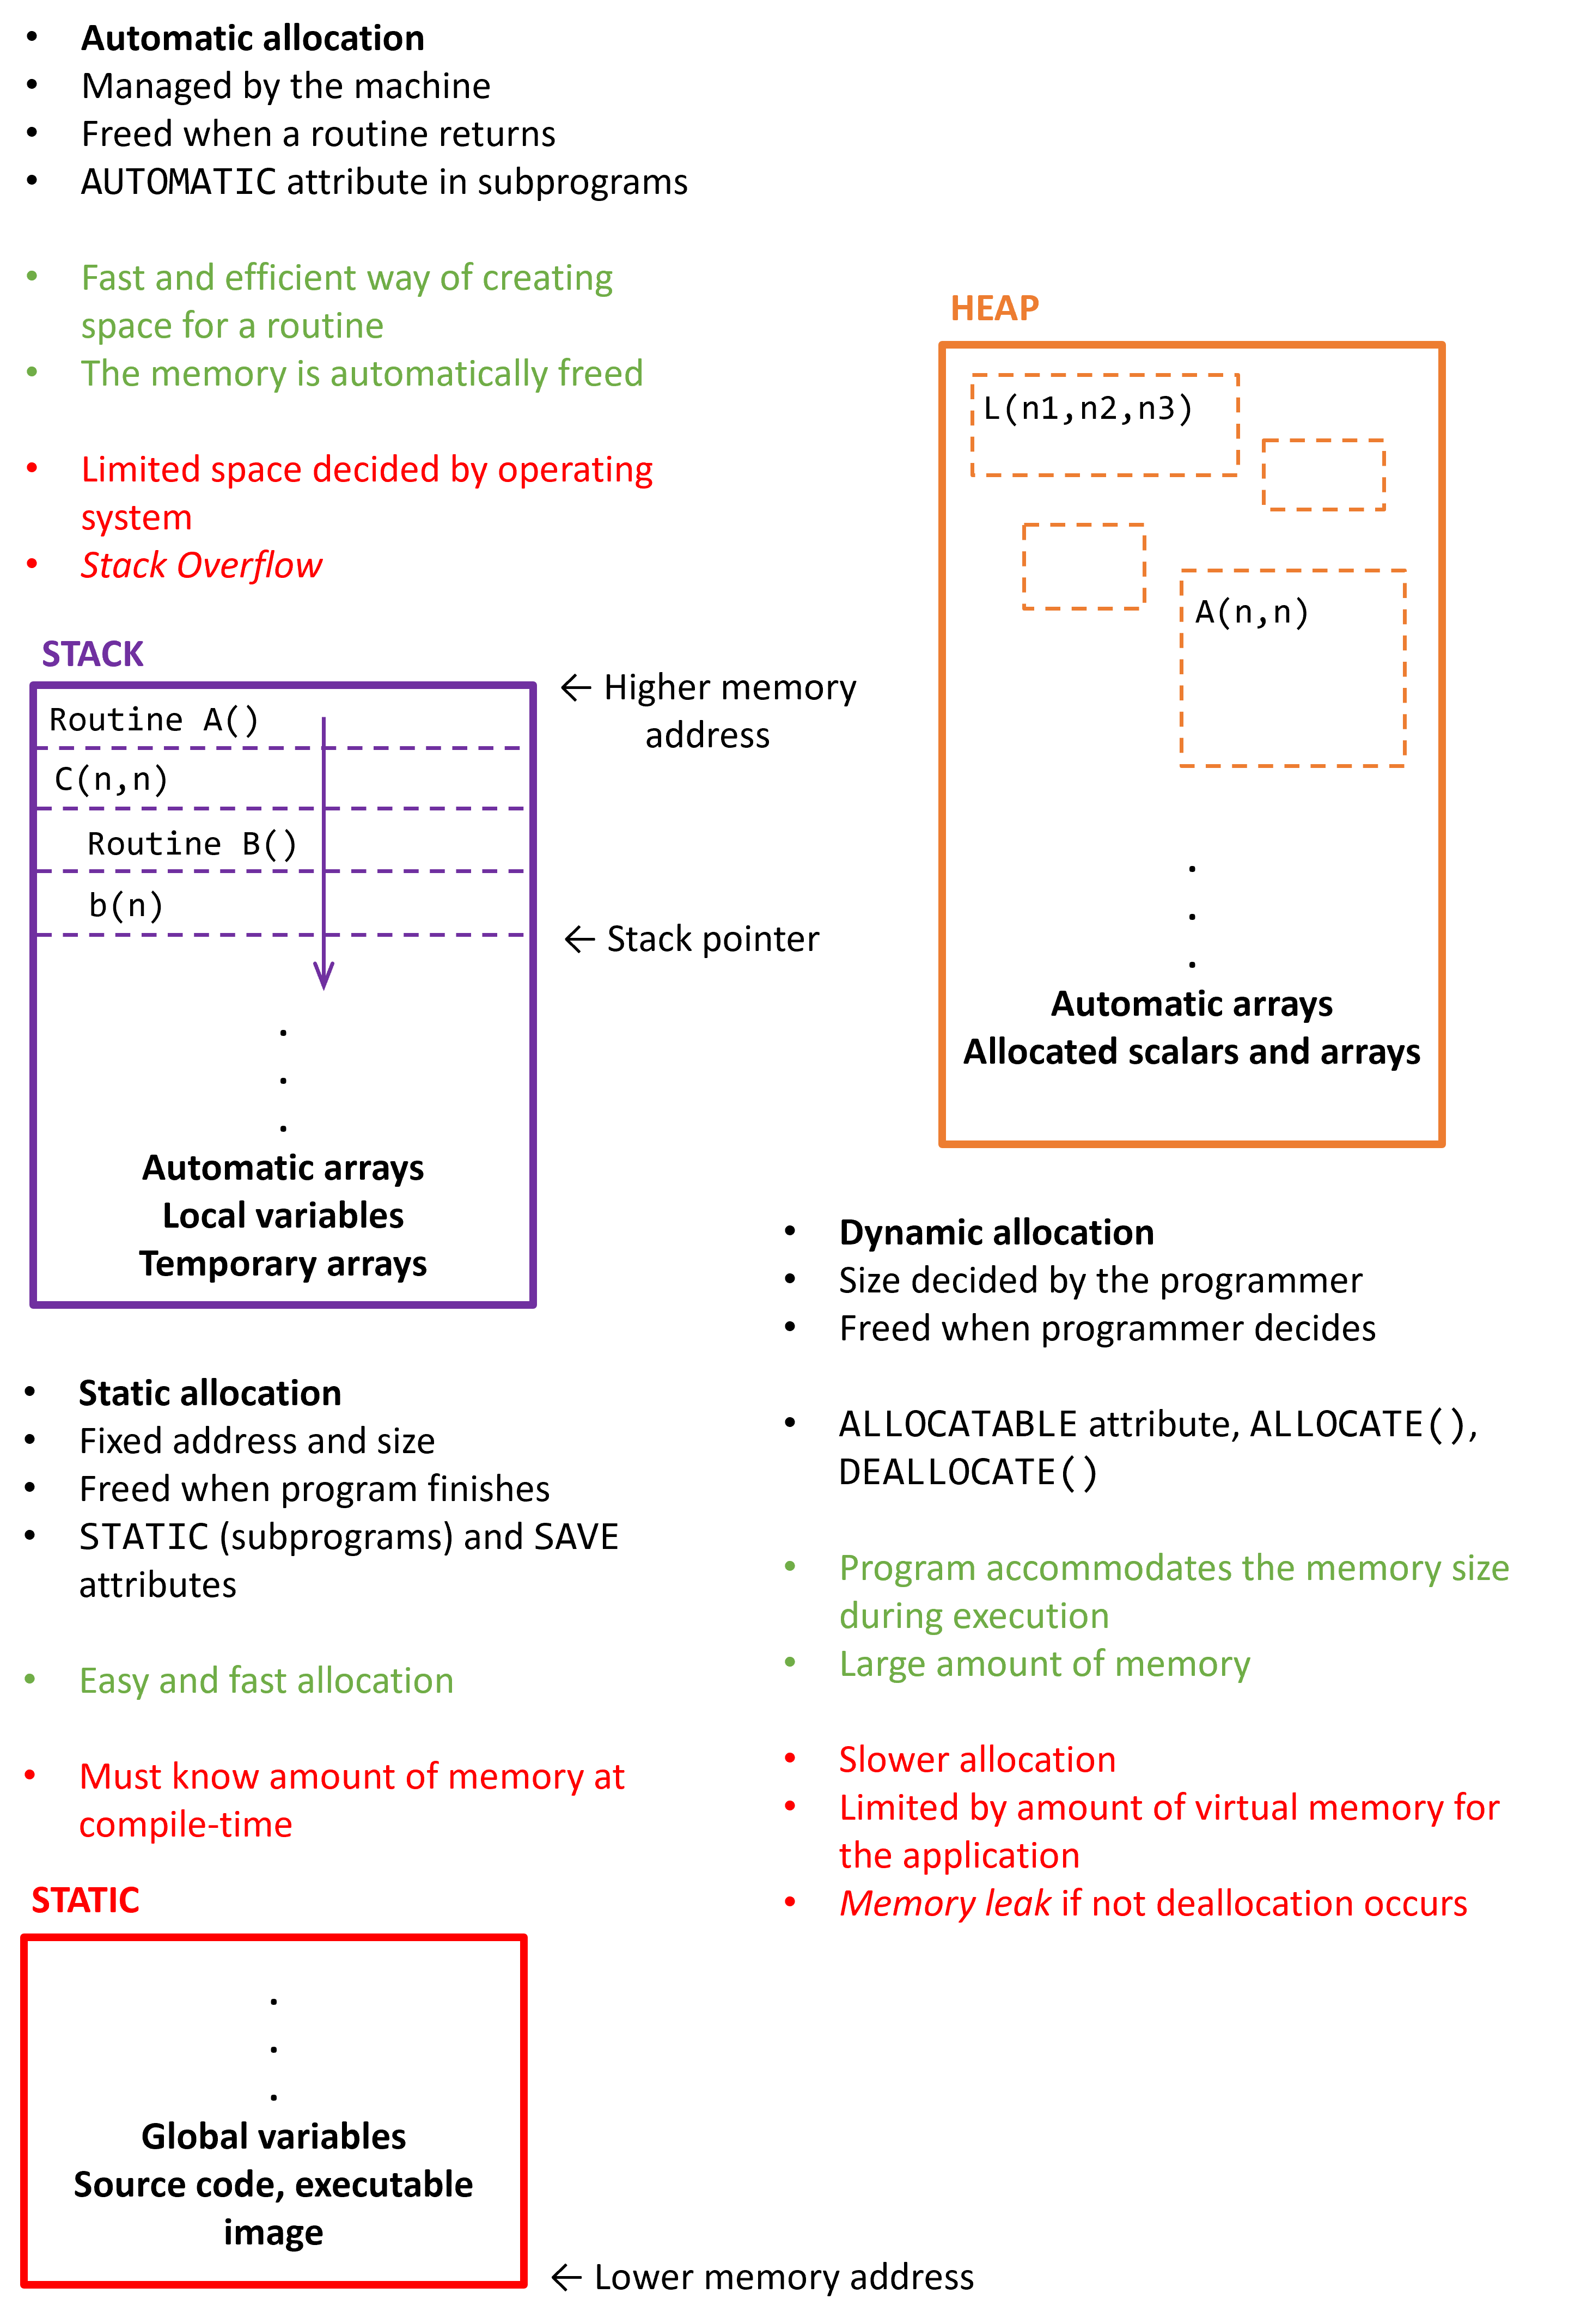
\includegraphics[width= \textwidth]{./doc/Figures/Memories.png}
    \caption{Three memory regions used by a program and the advantages and disadvantages associated to their allocation.}
    \label{fig:Memories}
\end{figure}






%-------------------------------------------------------------------------------------------------------------
%MAYBE INTERESTING IN FUTURE:

%When using AUTOMATIC, SAVE, STATIC, etc.
%\item How to manage it in your program and recommendations.
%\item How to reserve more space in each of them.


%-------------------------------------------------------------------------------------------------------------
%Revise the following concepts:
%
%\begin{enumerate}
%    \item Who manages the memory.
%    \item Where are physically stored (RAM, swap).
%    \item Which is faster to allocate and use.
%    \item Common problems related to the use of that memory.
%    \item How to manage it in your program and recommendations.
%    \item How to reserve more space in each of them.
%    \item etc.
%\end{enumerate}


%  Fortran for example uses this memory to create space for local arrays (those based on arguments of routines) or for temporary copies in array expressions. 
%     the stack is managed by the CPU, there is no ability to modify it
% variables are allocated and freed automatically

%  under the \texttt{deallocate} statement (in the case of Fortran)
  
         %___________________________________________________________________________________________________
\chapter{Operations with functions}     \label{chap:opfuncs}

    \section{Introduction} 

One of the paradigms grouped within the declarative programming is the functional programming paradigm,
which finds its bases in mathematics and more specifically in lambda calculus.
With this paradigm every piece of code uses pure mathematical style and is built 
under two main ideas: the functions are only applied to arguments 
and the functions are combined to create new functions. 

Some programming Languages that support functional programming are 
Haskell, JavaScript, Lisp, Erlang or Scala.
Although Fortran and Python are not functional programming languages, they
take several principles and ideas from this paradigm such as pure functions or first-class/higher-order functions,
the latter, introduced below, is intensively used in this chapter. 

%f matematica vs f lambda
In mathematics a function is a relation 
from elements of a set $X$ of inputs (domain) 
to elements of a set $Y$ of outputs (codomain) 
where each input is related to exactly one output.
$$ 
\myfunc{ f }{X}{Y}{x}{f(x) = x^2} 
$$
\newpage
A function in a language like Fortran follows the same concept:
\begin{verbatim}
function f(x) 
    real, intent(in) :: x
    real :: f

    f = x**2
    
end function
\end{verbatim} 
Notice that, in lambda calculus and functional languages, functions are much the same but anonymous, 
which means they do not have an identifier associated to denote them. 

This chapter covers the equivalent of some mathematical analysis tools translated to scientific programming. 
Piecewise-defined functions, plotting of functions, integrals and derivatives or series expansions of functions 
are some of the first things that a scientific programmer should know to solve problems. 
All these tools, when expressed in a program, can make intensive use of higher-order functions: 
those functions that can take one or more functions as arguments 
or can return a function as a result.

The examples presented here are developed with Fortran and Python, however, the concepts are cross languages. 
For example, the ideas around the approximation of a derivative or integral with a computer or 
the consequences of using finite precision to represent real numbers
are similar in any language. 

 
%Its properties are covered later in the Advance Programming chapter. 
%Try now to glimpse with these examples some of its advantages comparing it to the imperative programming.
%It seeks to have each line of code made up of mathematics which, 
%although it only needs from variables and functions to work, is extremely powerful.

%Modularity is a key property in a well-structured software, it simplifies debugging, allows to test independent pieces of code and code reuse.  
%Hence, considering the basic principles of the paradigm and the qualities inherited from being a declarative paradigm,
%functional programming has the potential to make a program 
%short, effective, easy and part by part debuggable, reusable, maintainable, testable, predictable, and well-structured among others. 

    %___________________________________________________________________________________________________
    \newpage
    \section{Defining piece-wise functions} \label{sec:piecewise}

A function can be defined by means of one or more formulas, a list of values, a recurrence rule, etc. 
In this example, the following piece-wise mathematical function is defined in Fortran 
using three formulas for different intervals of its domain:

$$ 
\myfunc{ f }{\mathbb{R}}{\mathbb{R}}{x}{f(x)} 
$$

$$
f\left( x\right) = 
\begin{cases}
     0,  \ \ \ \  \ \ \ \ \  x < -\frac{\pi}{2}       \\
     \cos(x), \ \             x \in\left[ -\frac{\pi}{2}, \frac{\pi}{2}   \right)        \\ 
     0, \ \ \ \  \ \ \ \ \   x \geq \frac{\pi}{2}
\end{cases}
\label{eq:piecewise}
$$

It can be easily done through a conditional expression on the variable $ x $ so, for each point of the domain the proper result is returned. 
From the numerical point of view two precautions must be taken into account:

\begin{itemize}
    \item In the first place, make sure that the entire domain of the function 
    is represented in the code, do not forget to consider all the intervals. 
    It is possible that the domain of the function is not the whole set $\left\{ \mathbb{R} \right\} $, 
    however, the function in the code may be called with values $ x $ out of the domain. 
    A big topic is opened under this premise; how can be the output of an out-of-domain value managed.
    
    \item In the second place, for the algorithm the order in which we define the 
    intervals is important. Consider what function we would be representing if the 
    conditional \texttt{( x < PI/2 )} is written in the first place
    and the conditional \texttt{( x < -PI/2 )} in the second place for this same example.
    
\end{itemize}


\newpage
%\vspace{0.5cm} 
\renewcommand{\home}{./Fortran/sources/Foundations/Calculus}
\listings{\home/Examples/Integrals_derivatives.f90}{function Piecewise_f}
{end function}{Integrals_derivatives.f90}

\vspace{-0.7cm} 
\subsection*{Python code} 
The same code written with Python is more straight-forward,
this function definition with an \texttt{if/else} structure is a good example. 
Remember that implicit typing can make programming simpler but can also lead to unpredictable results or errors difficult to debug.
\vspace{0.3cm}
\renewcommand{\home}{./Python/sources/Foundations/Calculus} 
\lstpython
\listingsp{\home/Examples/Integrals_derivatives.py}{def Piecewise_f}
{x > pi}{Integrals_derivatives.py}
\lstfor


    %___________________________________________________________________________________________________
    \vspace{-0.5cm}
    \section{Plotting functions}

For a mathematical function its graph is one of the ways to represent it. 
Notice that for a given function $ f(x) $ the set of all pairs 
$ \left\{ ( x, f(x) ) \mid x\in D \right\}$ (where $D$ is the domain of the function) 
are unique.

This is specially useful when the domain and codomain of the function are subsets of $\mathbb{R}$
or maybe the domain is a subset of $\mathbb{R}^2$ since the elements $(x,y)$ or $((x,y),z)$ can be 
associated to points in a coordinate system resulting in a curve in 2 dimensions or a surface in 3 dimensions. 
The graph of functions, results, variables, etc. is used for ``graphic debugging'', an essential way to debug 
scientific programs like simulations in physics. 
It makes much easier to find all kind of bugs in a program 
by means of plotting final or intermediate results obtained by the computer.  

The following example is based on DISLIN, a plotting library for Fortran and C languages created by the
Max Planck Institute. It is a high-level plotting library for displaying
data that can be called from the main program or subroutines.

\vspace{0.5cm}
\renewcommand{\home}{./Fortran/sources/Foundations/graphs} 
\listings{\home/plotting.f90}{subroutine plot}
{end subroutine}{plotting.f90}
\renewcommand{\home}{./Fortran/sources/Foundations/Calculus} 

\vspace{-.5cm}
The previous subroutine allows to plot a 201 points curve from a generic function declared (by means of an interface) as a:
$$ 
\myfunc{ \texttt{f\_R\_R} }{\mathbb{R}}{\mathbb{R}}{x}{\texttt{f\_R\_R(x)}} 
$$

It is used in combination with an initialization subroutine for the graph and a subroutine that displays the result (the Fortran solution that accompanies this book shows some examples of how to use this subroutines and DISLIN libraries):

\texttt{subroutine plot\_ini( xmin\_, xmax\_,  ymin\_, ymax\_ )} 

\texttt{subroutine plot\_show(  )}

Notice how this subroutine makes use of the \texttt{parameter M} that needs to be converted to \texttt{real} when the grid \texttt{x} is calculated to avoid operating in the integer field. Also, the use of implicit loops greatly simplifies the reading of the code.






    %___________________________________________________________________________________________________
    \newpage 
    \section{Integrals and derivatives of functions}   \label{sec:intder}

Let's build a simple approximation to the derivative of a function $ f(x) $ by means of its definition:

$$
f'(x) = \lim_{h\rightarrow 0}\frac{f(x+h)-f(x)}{h}
$$

In calculus, the existence of this limit (derivable function) implies that both lateral limits exist, are finite and equal (at least when the function is defined in both sides of the point $x$):

$$
    f'(x) = \lim_{h\rightarrow 0^-}\frac{f(x+h)-f(x)}{h} = \lim_{h\rightarrow 0^+}\frac{f(x+h)-f(x)}{h}
$$

To obtain an approximation to this value $ f'(x) $ in a point $x $ with the computer, finite differences can be used. Instead of reproducing the limit in the point, a fixed value of $ h \neq 0$ is used. Notice that both $ h > 0 $ or $ h < 0 $ are possible so the approximation can be found like a forward difference or a backward difference. Actually, also central differences can be used if the expression is slightly modified. What must be considered is that now each expression leads to a different approximation while in calculus the existence of the derivative implies that all values are equal. 

For this case let's consider $ h > 0 $ with $h$ a small value:

$$
    f'(x) \simeq \frac{f(x+h)-f(x)}{h}
$$

The question that arises; is it possible to bound the error of the approximation? 

$$
    E = f'(x) - \frac{f(x+h)-f(x)}{h}
$$

If the function $f(x)$ is sufficiently smooth near $x$ (for a forward-difference twice differentiable is needed), then a Taylor expansion can be used so the order of the scheme used is obtained. Intuitively, it is clear that by lowering the value of $h$ a better approximation of the derivative is obtained. Finding the order of the scheme means precisely finding how fast the error tends to zero when $h\rightarrow 0$. In addition, round-off error appears in this approximation depending on the value of $h$ too.

Let's bound the truncation error for a forward difference. Starting with the Taylor series of $f(x)$ at the point $x$ particularized in $x+h$:

$$
f(x+h) = f(x) + h f'(x) + \frac{h^2}{2} f''(x) + \mathcal{O}(h^3) 
$$

Notice that $\O(h^3)$ means that the following terms are lower than a constant times $h^3$. Re-arranging the expression:

$$
\frac{f(x+h) - f(x)}{h} = f'(x) + \frac{h^2}{2h} f''(x) + \mathcal{O}(h^2) = f'(x) + \frac{h}{2} f''(x) + \mathcal{O}(h^2) 
$$

$$
\abs{\frac{f(x+h) - f(x)}{h} - f'(x)}  \  \leq  \    C h  
$$

The error committed by replacing the derivative $f'(x)$ by the finite difference approximation is of order $h$ and the same result is obtained if backward-difference is used. Of course this is not the only way to approximate the value of a derivative. First of all, central differences could be used and, if the function is three times differentiable the truncation error of that approximation can be demonstrated that is of order $h^2$. Secondly, higher order finite differences exist so the value of a first derivative can be approximate with order $h^4$, $h^6$, etc. considering more points of the domain, while the example shown here comes from the derivative definition or the Taylor series expansion similarly, higher order approximations can be inferred from the interpolation theory. Thirdly, other strategies that also comes from the interpolation theory can be used so spectral convergence can be obtained (see section \ref{sec:convergence}). 

A different source of discrepancy between the real value and the approximation appears; round-off error, also dependent on the value of $h$ taken. Notice that as $h$ gets smaller, the values of $f(x+h)$ and $f(x)$ become more similar. This issue, with infinite precision arithmetic would not pose any problem, however, performing the subtraction with the computer's finite precision involves the problem of numerical cancellation. This topic is broaden in the chapter \ref{sec:cancellation} since the basis of real numbers representation are explained. For now, just keep in mind the following:

\begin{itemize}
    \item Every real numbers in the computer is stored with a rounded value that fits in the finite precision used by the computer. Consider for example the numbers $1.2345651$ and $1.2345649$, in a finite precision machine they could be stored only with 6 significant digits and they would become: $1.23457$ and $1.23456$, they have been rounded. Of course, both values $f(x+h)$ and $f(x)$ in our derivative computation suffer from this issue.
    
    \item When two near values are subtracted the significant digits are reduced, i.e. from 6 significant digits in the following expression we end up with just 1: 
    
    $$
    1.23457 - 1.23456 = 0.00001 = 1\cdot 10^{-5}
    $$
    
    \item If both values are approximated to the sixth digit and the result of the subtraction is a value in the order of magnitude imposed by that digit, then it is dominated by the round off made to the numbers!
     In this example the infinite precision operation would result in $1.2345651 - 1.2345649 = 2\cdot 10^{-7}$ quite smaller than the result obtained by the finite precision machine. 
\end{itemize}

Our expression for the derivative $\frac{f(x+h)-f(x)}{h}$ will have an error in the numerator divided by $h$ so, with no deeper explanations let's say now that this rounding error can be bounded by the following expression. Notice how it depends inversely on $h$ so it is a barrier for the reduction of h as a way to increase the accuracy of the derivative. The decision and meaning of writing $2\epsilon$ for the numerator error is deeply treated in the chapter \label{chap:reals}.  

$$
E_{round} = \frac{2\epsilon}{h}
$$

Since we could be interested in making $h$ as small as possible to obtain better approximations to the derivative, it is not difficult to find that round-off barrier in our computations. Both sources of error can be dominant and it is essential to understand the origin of both and how to relate the precision desired for a simulation (needs of the project) and the way to approximate derivatives with the computer. 

%------------------------------------------------------------------------------------------
The following codes recycles the procedure interface used along this chapter of \texttt{f\_R\_R(x)} for the function \texttt{f} and defines the \texttt{Derivative} function with inputs the function to derive and the value where obtaining the approximation. Notice that this new function itself also responds to the interface:

$$ 
\myfunc{ \texttt{f\_R\_R} }{\mathbb{R}}{\mathbb{R}}{x}{\texttt{f\_R\_R(x)}} 
$$

\newpage
\vspace{0.5cm}
\listings{\home/Calculus.f90}{Derivative}
{end function}{Calculus.f90}

\vspace{0.5cm}
\listings{\home/Calculus.f90}{interface}
{end interface}{Calculus.f90}


%------------------------------------------------------------------------------------------

Now let's compute the definite integral of a function $f(x)$ in the closed interval $ [a,b] $ and let's do it in a functional way as it is common during this book.
In this case we are going to obtain an approximation to the integral value through a Riemann sum, which means that the area of the curve under the function in the interval is obtained as a sum of small rectangles along the interval and carrying that process to the limit. 

$$ 
\int_{a}^{b}f(x)dx   =   \lim_{m\rightarrow \infty}\sum_{i=0}^{m-1}f(x_i) \Delta x
$$

Each value $x_i$ is taken from a partition of $[a,b]$:

$$
x_i = a + i\Delta x \ \ \    \text{with} \ \ \  i = 0, ..., m-1
$$ 

and with:

$$
\Delta x = \frac{\mid b-a\mid}{m}
$$

However, we need an approximation so instead of evaluating that limit, we choose a value $m$ big enough to accomplish with the accuracy required. 

$$ 
\int_{a}^{b}f(x)dx   \simeq \sum_{i=0}^{m-1}f(x_i) \Delta x
$$

In this example, the leftmost value of each subinterval is taken to approximate the rectangle area, however, the rightmost value or another point contained in the interval could be used. 

%------------------------------------------------------------------------------------------

\vspace{0.5cm}
\listings{\home/Calculus.f90}{Integral}
{end function}{Calculus.f90}

Some notes should be taken from this example: firstly, notice that the initial value given to \texttt{dx} is not the actual value used, it is just an approximation to the expected value  (\texttt{0.001}). The operation \texttt{abs(b-a)/dx} is used to calculate the approximate number of subintervals that fit in our interval $[a,b]$ and then the integer part is retained. Then, the exact value of  \texttt{dx} is calculated for an integer number of subintervals. Secondly, notice that the sum must not stop in the last value of the interval ($b$) but in the previous one since the area of that rectangle is computed by $dx\cdot f(a+dx(m-1))$. As usual, the whole addition can be compacted in the sum of the components of a vector defined by an implicit loop. 


\newpage 
\subsection*{Python code} 
Find the same example coded with Python, there is no need of explicitly declare an interface between the argument function \texttt{f} and the functions \texttt{Derivative( f, x )} and \texttt{Integral( f, x )}. 
\renewcommand{\home}{./Python/sources/Foundations/Calculus}

\vspace{0.5cm}
\lstpython
\listingsp{\home/Calculus.py}{def Derivative}
{return}{Calculus.py}
\lstfor

\vspace{0.5cm}
\lstpython
\listingsp{\home/Calculus.py}{def Integral}
{return}{Calculus.py}
\lstfor

 



    %___________________________________________________________________________________________________
    \newpage 
    \section{Examples of operations with functions}

The following subroutine gives some examples of the functions seen during this chapter. 
DISLIN is used for all the graphs as mentioned before. Firstly, the plot intervals must 
be initialize so the \texttt{plot\_ini} subroutine is used and the plotting boundaries 
are declared, all the graphs will be calculated and represented in 
$x\in \left[ -2\pi, 2\pi \right]$, 
$y\in \left[ -2.5, 2.5 \right]$.
Then, four functions are represented; a sine, 
the piecewise function defined in \ref{eq:piecewise},
its derivative and 
its integral from $-1$ to x. 

To graph those functions with \texttt{plot( f )}, the single input argument needed is the function itself.  
Also, the already explained \texttt{procedure (f\_R\_R) :: f} is used for \texttt{f}. Hence,
the functions \texttt{Derivative\_f(x)} and \texttt{Integral\_f(x)} are needed to 
build the following mathematical expressions: 

$$
\text{\texttt{Derivative\_f}}(x) = \frac{df(x)}{dx}
$$

and:

$$
\text{\texttt{Integral\_f}}(x) = \int_{-1}^{x} f(x) dx
$$

Remember that $f(x) = \text{\texttt{Piecewise\_f(x)}}$. Notice that integrating the function with these limits implies finding one of the primitive functions of $f(x)$, that one where the not defined constant has a specific value decided by the lower integration limit $x=-1$. The function treated in this example is positive (or zero) in the whole domain of definition so its integral as well. However, since it is plotted starting in $x = -2\pi$ and the function is integrated from $x=-1$, we expect the result to be negative until it reaches zero in $x=-1$ according to this property of definite integrals:

$$
\int_{-1}^{x} f(x) dx = - \int_{x}^{-1} f(x) dx
$$

\newpage 
\vspace{0.5cm}
\renewcommand{\home}{./Fortran/sources/Foundations/Calculus}
\listings{\home/Examples/Integrals_derivatives.f90}{Integral_and_derivative_examples}
{end subroutine}{Integrals_derivatives.f90}
 
 \newpage 
 \subsection*{Python code} 
 \renewcommand{\home}{./Python/sources/Foundations/Calculus}
 \lstpython
 \listingsp{\home/Examples/Integrals_derivatives.py}{def Integral_and_derivative_examples}
 {end}{Integrals_derivatives.py}
 \lstfor
 

    %___________________________________________________________________________________________________
    \section{Series expansion} 

One of the main focus of numerical methods is to approximate functions by means of different expansions: 

\begin{enumerate} 
\setlength\itemsep{-0.1cm}
	\item Polynomial expansion: Taylor, Lagrange.
	\item Trigonometric series: sine and cosine expansions. 
	\item Expansion by means of known basis: Chebyshev, Legendre, etc. 
\end{enumerate} 

The same function can be expanded or approximated with different basis.
It goes without saying that the computer only allows to sum a finite number $ N $  of terms. 

Hence, the best election is related to the rate of convergence 
of the expansion. In other words, given a tolerance error between the approximation and the exact function, 
the best expansion allows to obtain the approximation with a minimum number of terms $N$. 



        %___________________________________________________________________________________________________
        \newpage
        \subsection{Taylor expansions of functions} 
   
One of the most used series expansion of a function is its Taylor series, without going any further, in section \ref{sec:intder} we have used 
a Taylor expansion to estimate the truncation error committed when approximating the derivative of a function by its finite difference 
expression.

In general, as already mentioned, a series expansion is a very useful way to approximate the value of a given function in a domain. More 
specifically, the Taylor series, which uses power series, allows us to estimate the value of a function at one point from its value and the 
value of its derivatives at a different point. Polynomials are extensively known and they are easy to derive, integrate, multiply, etc. so 
treating a function as its power series approximation can have many advantages when it comes to operating with that function.

A power series of the function $f(x)$ (centered in $x_0 = 0$ and with $N+1$ terms) can be expressed as:
%\[  f(x) = \sum_{k=0} ^N a_k \  x^k, \qquad \qquad a_k = \frac{  f^{(k)} (0)  }{ k! },  \]  
 
\[  f(x) \approx \sum_{k=0} ^N a_k \  x^k,  \] 

where $a_k$ are real numbers that depend only on $k\in \mathbb{N}$ and not on $x$. These coefficients are calculated as:

$$
a_k = \frac{  f^{(k)} (0)  }{ k! }  
$$

being $f^{(k)} (0)$ the \textit{k}-th derivative of $f(x)$ in the point $x_0 = 0$.
 
For a Taylor expansion around a generic point $x_0$ the shape of the polynomial series and the coefficient expressions are:

\[  f(x) \sim \sum_{k=0} ^N a_k \  (x - x_0)^k, \qquad a_k = \frac{  f^{(k)} (x_0)  }{ k! }   \] 





Let's take a look at the Taylor expansion functions proposed here (written with a declarative style). Two approximations are used, one is 
called under the expected minimum value to be added to the series (epsilon), the other is directly called with the number of terms to be 
added. Imitating a multilayer structure, previous functions can be recycled, for example \texttt{TaylorE} needs to sum as many terms as the 
epsilon value requires so the function \texttt{Sigma} function (seen in chapter \ref{sec:Sigma}) is used. In a different way, 
\texttt{TaylorN} is directly based on \texttt{Sigma\_N} since the number of terms to be added are known and declared as an argument.

Despite that, the structure of both functions is the same, a declaration of the Taylor expansion definition. The \texttt{Sigma} function is 
called with the general term of the series, the first term to add (which is 0 in this kind of power expansion) and the condition to stop 
(epsilon value or number of terms). Those are the only ingredients needed to compute the sum series that returns the value of the Taylor 
expansion in a point $x$. 
  
\vspace{0.5cm}
\renewcommand{\home}{./Fortran/sources/Foundations/Calculus} 
\listings{\home/Taylor_expansions.f90}{function TaylorE}
   {end function}{Taylor_expansions.f90}
   
\renewcommand{\home}{./Fortran/sources/Foundations/Calculus}       
\listings{\home/Taylor_expansions.f90}{function TaylorN}
   {end function}{Taylor_expansions.f90}
   

\newpage   
A couple of details should be noticed here. First of all, the derivatives of the function to be expanded are introduced as an argument in 
\texttt{Taylor} function. The arguments of this function must be the value where deriving and its order. To do that, a generic procedure is 
used so it can be recycled next time a function of the same form is used:

$$ 
\myfunc{ \texttt{f\_RxN\_R} }{\mathbb{R} \times\mathbb{Z}}{\mathbb{R}}{\left( x,k \right)}{\texttt{f\_N\_R(x,k)}} 
$$
   
Secondly, both functions are overloaded into one called \texttt{Taylor} so the particularities of each one are transparent for the user, just 
call a generic function specifying an epsilon value or a number of terms as fourth argument, the calculation is correctly performed 
automatically. Notice that the \texttt{type} of argument must always be respected so \texttt{N}, the number of terms, must be an 
\texttt{integer} value and \texttt{eps}, on the contrary, must be a \texttt{real} value.  
   
    
\vspace{0.5cm}   
\renewcommand{\home}{./Fortran/sources/Foundations/Calculus} 
\listings{\home/Taylor_expansions.f90}{interface}
   {end interface}{Taylor_expansions.f90}

\renewcommand{\home}{./Fortran/sources/Foundations/Calculus}  
\listings{\home/Taylor_expansions.f90}{interface Taylor}
         {end interface}{Taylor_expansions.f90}
   

\newpage 
Let's consider the following four examples (included in the Fortran project attached to this book) to better visualize how this function 
works:

\vspace{0.3cm}
\renewcommand{\home}{./Fortran/sources/Foundations/Calculus} 
\listings{\home/Examples/Series_expansion.f90}{Taylor_expansion_examples}
{contains}{Series_expansion.f90} 

\vspace{-0.2cm}
The first block of code calculates the value of $e$ using a Taylor expansion of the function $e^x$ in $x_0 = 0$. Take a look at the source 
code to check how the derivative of the function is implemented.  Three calls are performed with $N = 1$, $N = 4$ and $eps = 1e-7$. As it is 
expected, each result returns a better approximation to the value of $e = 2.7182818284...$:
\begin{verbatim}
Taylor exp(1.) x0=0   :   2.00000000000000
Taylor exp(1.) x0=0   :   2.70833333333333
Taylor exp(1.) x0=0   :   2.71828182619849
\end{verbatim}
   
The other three blocks of code compare some functions with their Taylor series expansions. In the first place a cosine function is compared 
with its Taylor expansion around $x_0 = 0$ using $N = 10$ (11 terms of the series). The plot shows a black cosine curve in the interval 
$\left[0,2\pi\right]$ compared with a red curve with its series expansion (figure \ref{fig:Taylor1}). The same, with $N = 5$, is done with 
the function $f(x) = \frac{1}{1-x}$ in the interval $\left[-2,2\right]$, the result is seen in the the figure \ref{fig:Taylor2}. Finally, the 
cosine is approximated by 7 different curves, each of them considering more terms of the series expansions ($N = 1, 5, 9, 13, 17, 21$ and 
$25$) so the result converges to the cosine function (figure \ref{fig:Taylor3}). 

\begin{figure}
    \begin{subfigure}[h]{0.4\textwidth}
        \centering
        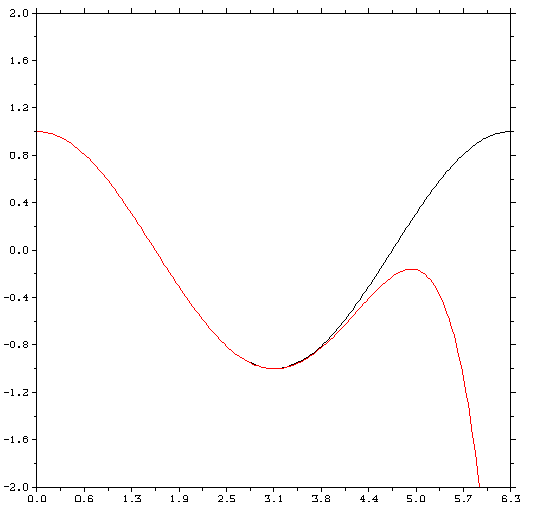
\includegraphics[width = \textwidth]{./doc/Figures/Taylor1.png}  \\
        \caption{Cosine (black) and Taylor expansion around $x_0 = 0$ with $N = 10$}
        \label{fig:Taylor1}
    \end{subfigure}
    \hspace{\fill}
    \begin{subfigure}[h]{0.4\textwidth}
        \centering
        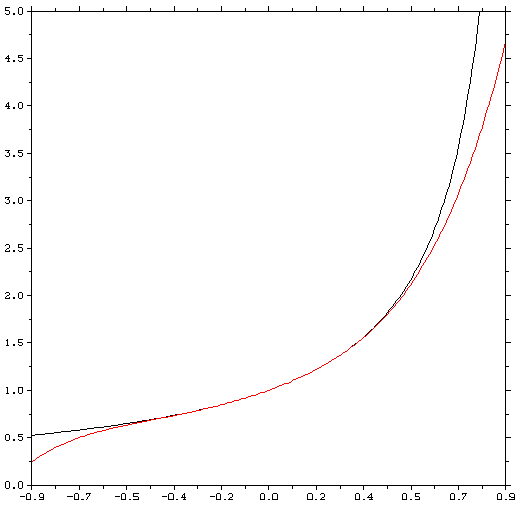
\includegraphics[width = \textwidth]{./doc/Figures/Taylor2.png}  \\
        \caption{Function $f(x) = \frac{1}{1-x}$ (black) and Taylor expansion around $x_0 = 0$ with $N = 5$}
        \label{fig:Taylor2}
    \end{subfigure}    

    \centering
    \begin{subfigure}[h]{0.4\textwidth}
        \centering
        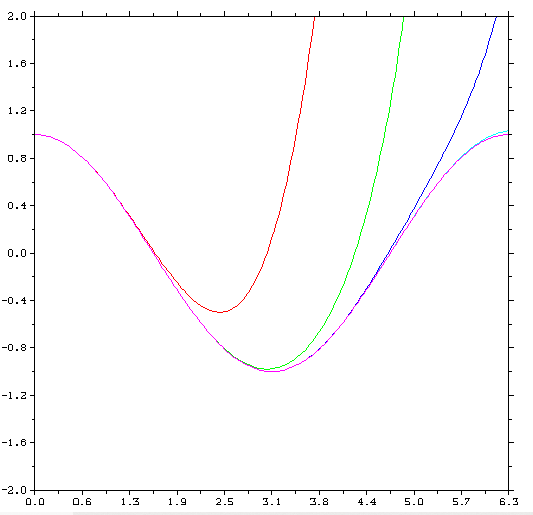
\includegraphics[width = \textwidth]{./doc/Figures/Taylor3.png}  \\
        \caption{Cosine (black) and different Taylor expansions around $x_0 = 0$ with $N = 1, 5, 9, 13, 17, 21$ and $25$}
        \label{fig:Taylor3}
    \end{subfigure}
    \caption{Different Taylor expansions for functions.}   \label{fig:Taylor}
\end{figure}


  
 
            \newpage 
            \subsubsection*{Python code} 
 The same functions are coded now with Python, notice that overloading both into one function called \texttt{Taylor} is performed in a 
 different way.
 
 \vspace{0.5cm}
 \renewcommand{\home}{./Python/sources/Foundations/Calculus} 
 \lstpython
 \listingsp{\home/Taylor_expansions.py}{def Taylor}
 {exit}{Taylor_expansions.py}
 
 
 \listingsp{\home/Taylor_expansions.py}{def Taylor_e}
 {Sigma}{Taylor_expansions.py}
  

 \listingsp{\home/Taylor_expansions.py}{def Taylor_N}
 {Sigma}{Taylor_expansions.py}
  
 
    
   
   \newpage 
   Try the same examples treated with Fortran in the Python project attached to this book:
      
   \vspace{0.5cm}
   \listingsp{\home/Examples/Series_expansion.py}{def Taylor_expansion_examples}
   {end}{Series_expansion.py}
   \lstfor
   
   
   
   
 % Taylor_expansion_examples
  
  
  
  
  
   
        %\newpage 
        %%___________________________________________________________________________________________________
        %\subsection{Parseval's identity} 
%
%Let's consider a function $f(x)$ and its Fourier series expansion, whether expressed as a sines-cosines expansion:
%\begin{equation} 
%	f ( x)  =  \sum_{k=0} ^{\infty} \  \hat{a}_k  \ \cos\left(k x\right)  + \sum_{k=1} ^{\infty} \  \hat{b}_k  \sin\left(k x\right)
%\end{equation} 	
%
%or as a complex form:
%\begin{equation} 
%    f ( x)  =  \sum_{k=-\infty} ^{\infty}  \hat{c}_k  e^{ i k x }
%\end{equation} 
%
%Notice that for this expressions the function $f(x)$ is considered real-valued and periodic with period $T=2\pi$. As we know, the computer 
%can not compute an infinite number of terms, we must truncate the series somewhere, let's say when $k = N-1$ so a total of $N$ terms are 
%considered. Then, the expansion becomes:
%\begin{equation} 
%    f ( x)  =  \sum_{k=0} ^{N-1} \  \hat{a}_k  \ \cos\left(k x\right) + \sum_{k=1} ^{N-1} \  \hat{b}_k  \sin \left(k x\right)
%\end{equation}
%
%or in complex form, those $N$ terms becomes:
%\begin{equation} 
%    f ( x)  =  \sum_{k=-\frac{N}{2}} ^{\frac{N}{2}-1}  \hat{c}_k  e^{ i k x }
%\end{equation} 
%
%We can quickly revise the relation between the coefficients of the sines-cosines expansion and the coefficients of the complex series 
%expansion:  
%
%$$
%\begin{cases}
%    \hat{c}_k  =  \frac{1}{2} \ ( \ \hat{a}_k  - i \ \hat{b}_k \ ),  \quad k=1, \ldots, N/2.   \\
%    \hat{c}_0  = \hat{a}_0   \\
%    \hat{c}_{-k}  =  \overline{ \hat{c} } _{k}  , \quad k=1, \ldots, N/2. 
%\end{cases}
%$$
%
%With that in mind, the Parseval's identity says:
%\begin{equation} 
%	\int _{-\pi} ^{\pi} f(x)^2 \ dx =  2 \pi  \sum_{k=-\infty} ^{\infty}  | \hat{c}_k | ^2       =  2 \pi \left(    | \hat{c}_0 |^2 + 2 
%	\sum_{k=1} ^{\infty} |  \hat{c}_k  |^2 \right) 
%\end{equation} 
%
%
%
%
%
%A good example, related to previous chapters, is the following: consider the function $ f(x) = x \quad $ $ \forall x \in [-\pi, +\pi ) $ and 
%extend it periodically to the right and to the left. Once $ f(x) $ is defined in this way, it can be approximated by a sine expansion: 
%%\begin{equation} 
%%	f ( x)  =  \sum_{k=1} ^{N/2} \   \hat{b}_k  \sin k x, 
%%\end{equation} 
%\begin{equation} 
%	f ( x )  =  \sum_{k=1} ^{\infty} \   \hat{b}_k  \sin \left(  kx\right), 
%\end{equation} 
%where the coefficients $ \hat{b}_k $ are given by:
%%\begin{equation} 
%%	\hat{b}_k   = \frac{ (-1)^{k+1} }{ \pi k }, \qquad k=1, \ldots, N/2. 
%%\end{equation} 
%\begin{equation} 
%    \hat{b}_k   = \frac{ 2 (-1)^{k+1} }{ k }, \qquad k=1, \ldots,\infty. 
%\end{equation} 
%
%Using the Parseval's identity with $f(x)$:
%$$
%\int_{-\pi}^{\pi}  x^2 dx  = \frac{2}{3} \pi^3 = 2\pi \left(   2\sum_{k=1}^{\infty}  \mid  -\frac{1}{2} i \hat{b}_k   \mid ^2  \right)
%$$
%
%and the following summation is obtained: 
%%\begin{equation} 
%%	\sum_{k=1} ^{\infty} \  \frac{1}{n^2}  \  = \frac{\pi^2}{6}
%%\end{equation} 
%\begin{equation} 
%    \sum_{k=1} ^{\infty} \  \frac{1}{k^2}  \  = \frac{\pi^2}{6}
%\end{equation}
%

        \newpage 
        \subsection{Truncated Fourier series}
Fourier series are important expansions in applied mathematics or physics to represent a
periodic functions.  
When implementing these expansions in the computer, truncated Fourier series are used
to approximate the infinity Fourier expansion.  
A truncated Fourier series is a finite sum of sine and cosine waves. 
$$
f(x) = \sum_{k=0}^N a_k \ \cos( \ 2 \pi k  x \ ) + b_k \ \sin ( \ 2 \pi k  x \ ), 
$$
or expressed in its compact form: 
$$
f(x) = \sum_{k=-N/2}^{N/2-1} c_k \ e^{ \ 2 \pi k  x \ i } .
$$
If $ f(x)$ is real, $ c_k $ and $a_k,\  b_k$ are related with the following expressions: 
$$
c_k = \frac{1}{2}(a_k - i b_k), \qquad k=0, \ldots, N/2, 
$$
$$
c_{-k} = \overline{c_k},\qquad k=1, \ldots, N/2,
$$
where $ k $ represents different harmonics of frequency or wavelength  $ 2 \pi k $  of different 
 sine and cosine components.

The following saw-tooth wave: 
$$
f(x) =
\left\{
\begin{array}{ll}
\displaystyle                          
\frac{x}{\pi}, \hspace{1cm} \hspace{2cm} &  \displaystyle  0 \leq x \leq  \pi,      \\ \\
\displaystyle                                                            
\frac{x}{\pi} -2 ,  & \displaystyle    \pi < x <  2 \pi. 
\\                                                                                                 
\end{array}                                                                   
\right.                                                     
$$
is expanded in Fourier series
$$
f(x) =\sum_{k=1}^N  - \frac{2 \ (-1)^{k}}{\pi \ k}   \ \sin ( \ 2 \pi k  x \ ).
\label{sawtooth}
$$



        \newpage
        \subsubsection*{Fortran}
In following Fortran code, the saw--tooth wave is reconstructed 
by means of its harmonic decomposition. The function \verb|Fourier_series| implements 
equation (\ref{sawtooth}). Then,  subroutine \verb|Fourier_example| calculates the image of 
\verb|M=2000| points to plot the resulting graph. 
\vspace{0.5cm} 
\renewcommand{\home}{./Fortran/sources/Advanced_programming/functional programming} 
\lstfor 
\listings{\home/Fourier.f90}
{elemental function Fourier_series}
{end function}{Fourier.f90}
\vspace{0.25cm}
\listings{\home/Fourier.f90}
 {subroutine Fourier_example}
 {end subroutine}{Fourier.f90}


        \newpage
        \subsubsection*{Python}
In following Python code, the saw--tooth wave is reconstructed 
by means of its harmonic decomposition. The function \verb|Fourier_series| implements 
equation (\ref{sawtooth}). Then, function \verb|Fourier_example| calculates the image of 
\verb|M=2000| points to plot the resulting graph. 
\vspace{0.5cm} 
\renewcommand{\home}{./Python/sources/Foundations/Algebra} 
\lstpython
 \listingsp{\home/Fourier.py}
 {def Fourier_example}
 {plt.show}{Fourier.py}


\listingsp{\home/Fourier.py}
{def Fourier_series}
{return}{Fourier.f90}

  
  
  
         
\newpage   
\chapter{Reading and writing external files}    \label{chap:readwrite}



Reading and writing data from/to external files is usually an essential part of every software project. Maybe you want to process data returned by a different software, share information between two programs written in different languages, process the results from your program in an specialised plotting software or just reading the inputs of your program through a data sheet. 

The aim of this chapter is to propose an orderly way to encapsulate and use a matrix reading function. As a result, this function hides the particularities of Fortran (or any other programming language where imitating this function) related to reading/writing information from files and builds an useful tool that can be easily recycled for future projects. A one-time effort to create a powerful and general tool is worthwhile if you are using a programming language regularly. Additionally, encapsulating and separately validating this tool reduces failures and helps to standardize the way of proceeding each time that a reading operation is performed.

The following subroutine loads two matrices by declaring the relative path of the \texttt{.csv} file where information is stored and then writes them in the screen by rows. Notice that the dynamic object \texttt{A} in the subroutine does not need to be allocated since the compiler automatically takes care of that when the output of the reading function is available. Also, notice that the matrix is written using an explicit loop for rows and an implicit loop for columns. This technique is preferred since Fortran writes by default the data by columns. 

\newpage 
\vspace{0.5cm} 
\renewcommand{\home}{./Fortran/sources/Foundations/read files} 
\listings{\home/read_files.f90}{subroutine Test_load_matrix}
{end subroutine}{read_files.f90}


%-------------------------------
The function \texttt{load\_matrix()} is in charge of reading the data and assigning it to a local variable \texttt{A}. Contrary to the subroutine, here the dynamic object \texttt{A} is allocated by hand. 

In summary, this function opens the requested file (input argument), reads the first line and saves the information in the variable \texttt{header}. This header determines the number of columns in which the data is ordered (using commas as separators). From now on, all rows are read until the total number is determined and the size of array \texttt{A} can be defined. Finally, the whole file can be reread again, saving the data in \texttt{A} this time. This function makes use of an auxiliary function called \texttt{columns( string, s )} which reads how many columns are declared in the header of the file using some specific separator. 

Encapsulating some tools like this one allows the programmer to save time and reduce possible sources of error in future projects but does not eliminate the need to know the peculiarities of reading/writing data in files or screen, as is the case with any programming language. For the needs of each project some adjustments could be done.

\newpage
\vspace{0.5cm} 
\renewcommand{\home}{./Fortran/sources/Foundations/read files}
\listings{\home/read_files.f90}{function load_matrix}
{end function}{read_files.f90}

\renewcommand{\home}{./Fortran/sources/Foundations/read files}
\listings{\home/read_files.f90}{function columns}
{end function}{read_files.f90}

  
  
  
  
\newpage 
\subsection*{Python code} 
The following examples reproduce the same behaviour with Python, notice that many functions are already implemented in different packages of Python. 
In this case the function \texttt{load\_matrix()} encapsulates the load of the specific file through \texttt{read\_csv()} (included in Pandas package), prints the header and returns the needed values. As mentioned before, encapsulating tools like this one allows you to save time and reduce possible sources of error in future projects by creating an standard for all your programs. 


\vspace{0.5cm}
\renewcommand{\home}{./Python/sources/Foundations/Read_files}
\lstpython 
   \listingsp{\home/Read_files.py}{def Test_load_matrix}
    {end}{Read_files.py}
  
 \renewcommand{\home}{./Python/sources/Foundations/Read_files} 
    \listingsp{\home/Read_files.py}{def load_matrix}
     {return}{Read_files.py} 
  \lstfor
  
  
  
 %   A batch file named: \mycap{Preliminary_examples.bat} allows to compile and to run this main program.  
 
 
 % \newpage  
 
 
 
 
 %   \subsection{Windows}
 
 
 % _______________ RUN EXAMPLES_________________________________________________
 
 %   >compile_Cauchy_Problem_examples.bat
 %   
 %   >compile_BVP_examples.bat 
 %   
 %   >
 %   
 %   >
 %   
 %   
 %   
 %   Examples of use compile.bat 
 %   
 % %  _________BASIC USAGE___________________________________________________________ 
 %   
 % %  >compile main 
 %   
 %   The file main.f90 contains the main program to be executed
 %   
 %%   e.g. to compile and to execute the "hello world" first example 
 %   
 %   >compile main    
 %   
 %   
 % %  ___________ADVANCED USER______________________________________________________
 %   
 %   If the user develops a new module, or he wants to use existing examples,
 %   the compilation procedure is as follows: 
 %   
 %%   > compile module_name main 
 %   
 %   1) module_name is a fortran module file which is located in sources. 
 %   
 %   2) main file is the main program.
 %   It contains a use setence to access module_name and it calls some subrutine of  the module 
 %   
 %   
 %   e.g. 
 %   > compile 
 %   
 
 
 
 
 
 
 %   
 %   
 %   
 %   
 %   Informatics 2017/2018 Aerospace Engineering (UPM) 
 %   
 %   How to install FORTRAN and graphical windows in windows 10 
 %   
 %   Author: Juan A. Hernandez:  juanantonio.hernandez@upm.es 
 %   
 %   
 %   
 %   %   A) Copy Informatica\_2018 to Desktop 
 %   
 %   B) Check the compiler 
 %   1)open command prompt and type >compile Hello\_world
 %   2)open  command prompt and type >compile plot\_graph
 %   
 %   
 %   \subsection{Ubuntu}
 %   
 %   
 %   
 %   Informatics 2017/2018 Aerospace Engineering (UPM) 
 %   
 %   How to install FORTRAN and graphical windows in Ubuntu from windows 10 
 %   
 %   Author: Juan A. Hernandez:  juanantonio.hernandez@upm.es 
 %   
 %   
 %   
 %   
 %   A) Install UBUNTU from Windows 10 (skip this step if your machine is UBUNTU) 
 %   
 %   1) Setting/Security/Developer ( allow to create and modify programs ) 
 %   
 %   2) control panel/programs/Windows characteristics allow UBUNTU 
 %   
 %   3) cmd> bash . Create user and password UBUNTU machine 
 %   
 %   4) Install X11 server for graphical windows ( XMing ) to run graphical linux binaries from shell.
 %   Capability to start 64-bit GUI-programs from the desktop file manager 
 %   
 %   5) Install graphical vim editor to check: 
 %   
 %   \$sudo apt-get install vim-gtk
 %   
 %   Now, you?ll need to set the ?DISPLAY? environment variable to point at the X server running on your Windows 10 PC. 
 %   If you don?t do this, graphical applications will simply fail to launch.
 %   To do this, run the following command in the Bash environment:
 %   
 %   \$export DISPLAY=:0
 %   \$gvim
 %   
 %   
 %   B) Install gfortran 
 %   
 %   1) \$ sudo apt-get install gfortran 
 %   
 %   
 %   
 %   C) Install DISLIN to plot with UBUNTU 
 %   
 %   1)  should install OpenMotif on Ubuntu 
 %   
 %   
 %   \$ sudo add-apt-repository deb http://archive.ubuntu.com/ubuntu lsb\_release -sc universe multiverse
 %   
 %   \$ sudo apt-get update 
 %   
 %   \$ sudo apt-get install libxm4
 %   
 %   \$ sudo apt-get install libmotif4* libmotif-dev
 %   
 %   \$sudo apt-get install libx11-dev libxt-dev libgl1-mesa-dev  WARNING:(l1 ele and then one )
 %   
 %   
 %   2) Check the compiler 
 %   
 %   1)\$ ./compile.sh Hello\_world
 %   2)\$ ./compile.sh plot\_graph
 %   
 %   
 %   
 %   \subsection{MAC} 
 %   
 %   Informatics 2017/2018 Aerospace Engineering (UPM) 
 %   
 %   How to install FORTRAN and graphical windows in MAC OS 
 %   
 %   Author: Juan A. Hernandez:  juanantonio.hernandez@upm.es 
 %   
 %   
 %   1) How to execute a Terminal 
 %   
 %   Applications/ Utilities/ Terminal
 %   
 %   2) How to execute a Terminal in a specific folder
 %   
 %   System Preferences/ Keyboard/ Speed functions/ Services - scroll and select "Terminal in the folder"
 %   
 %   
 %   
 %   3) Install gFortran to compile
 %   
 %   3.1) Install manager HOMEBREW (https://brew.sh)
 %   3.2) \$ brew install gcc
 %   
 %   
 %   4) Install Openmotiff
 %   
 %   4.1) Install server X11 through XQuartz (https://www.xquartz.org)
 %   Capability to start 64-bit GUI-programs using x-windows from the shell 
 %   
 %   4.1)\$ brew install openmotif
 %    
         \chapter{Computer, programming languages and paradigms} 

%De qué va Foundations de forma historiada
This chapter is intended to give the reader more context about the concepts treated before.  
The following sections review some building blocks of the theory of computation 
through the names of the people that worked on them: Turing, Church, Neumann and Backus.

Notice that each section from 6.1 to 6.4 extends the concepts treated in chapters 1 to 4.
Concepts like model of computation, the Von Neumann architecture and how it influences a programming language are summarized in section \ref{sec:vonNeu}.
The main ideas behind the imperative and declarative programming paradigms are treated in section \ref{sec:impvsdec}.
Vector languages, another essential property desired for scientific computing are introduced in section \ref{sec:veclan}.
Section \ref{sec:fpro} gives a theoretical description for Functional Programming, a paradigm usually included within the declarative paradigms. 
 
Finally, the authors consider that a brief knowledge of the history of computers and programming languages 
allow to understand how different programming skills or paradigms have evolved during the last decades. 
For this reason, a pleasant history tour is proposed in section \ref{sec:films}. 
The birth of computers, the space race and the influence of profound mathematicians among other factors conformed the origin of computing languages. 
Several movies and documentaries are recommended to understand those naive and happy days and how geeks and nerds had a big influence in the first stages of personal computer business.
  
  
   
  %In this part, basic operations are presented as a first approach to 
  %perform simple mathematical operations.
  % to learn applied mathematics 
  %a chapter including  
  %In it the reader can become familiar to the use of basic sentences in order
  
  %Some notions of theory of computation are revised here so a reader that is new 
  %to the scientific programming can familiarize himself.
  
 

    \newpage   
    \section{Von Neumann style}  \label{sec:vonNeu}
    %\vspace{-0.3cm}
The theory of computation gives the basis for the automatic processing of information where there is a 
problem to solve (a function between a bunch of inputs and their associated outputs) 
and a machine (analog, digital, quantum, etc.) to solve it. 
The tools of the theory of computation tell 
if the problem can be solved in the \textbf{framework of a model of computation}, 
using an \textbf{algorithm} and 
\textbf{how efficiently} is going to be solved.

But first let's define what a model of computation is: a mathematical abstract construction 
that describes how to compute the output of a mathematical function given its input.
The Turing machine, invented by Alan Turing in 1936 by the name of ``a-machine'', is a model of computation. 
The purpose for this model of computation was to give answer to some essential questions 
in the theory of computation and mathematics in general. 

This abstract construction consists on a scanning head capable of reading from an 
infinite tape of cells, a single cell at a time. 
This tape has information coded and once a cell is read, the machine can delete that cell, 
write another symbol or leave the symbol. 
Then, it can move to a different position in the tape. 
According to the current state of the 
machine and the position in the tape the machine follow a set of rules (also coded) and take some action or another. 

Everything that is computable and everything that a machine can compute nowadays can be theoretically programmed in a Touring machine 
although maybe inefficiently. 
Furthermore, it is said that any system capable of doing what a Touring machine can do is Touring-complete and 
than can also compute everything that is computable. 
These ideas can be applied to programming languages apart from computers and,
given a computable algorithm, find if it can be implemented in the specific language.
It turns that all programming languages nowadays are Touring-complete as soon as they allow 
mainly if-then-else structures and go-to statements. 

Notice that a conceptual model of computation is intimately related not only to the 
real machines we use everyday from a hardware point of view (laptops, PCs, smartphones, etc.) 
but also to the programming language. 
Computers today are built by implementing what 
a Turing machine describes theoretically, using an architecture. 
The architecture is the set of rules and methods that describe how software 
and hardware are organized, interrelate and work to conform a machine.

%von Neumann architecture
The most common architecture used in the machines around us (although not the only option) is the von Neumann architecture. 
In this description of a computer, a Central Processing Unit (CPU) is in charge of executing the instructions that are stored in a Memory Unit (which is separated from the CPU). 
In that memory, with each memory position uniquely identified by an address, the data and program are stored together. 
Some Buses transfer data, addresses and control commands between different parts of the computer
and at the same time allows the communication with input/output devices.
Hence, in the simplest description of this architecture we have three elements; CPU, memory and a bus to transfer data between both. 
The CPU works following an instruction cycle composed by three stages:
\begin{enumerate}[label=(\roman*)]
    \item It fetches the next instruction of the program from the memory address (a counter points to this address),
    \item this instruction is decoded and 
    \item the CPU performs the actions required by the instruction (reading addresses, performing arithmetic, writing in memory, etc.)
\end{enumerate} 

According to John Backus in his article ``Can Programming Be Liberated from the von Neumann Style? A Functional Style and Its Algebra of Programs'' 
this bus that connects CPU and memory acts as a bottleneck. 
He says this is because in each instruction cycle the bus transmit a single word (let's say 64 bits) between memory and CPU.
The purpose of any program is to modify the content of the memory so at the end of the execution the output of our function (or problem to solve) is stored.
But this process is performed by pumping single words at a time through this bus.
In addition, from all the information sent back and forth, a large part is not useful for the solution of our problem: names of data, other data needed to compute those names, memory addresses, etc. 

Notice that this architecture not only describes how the hardware is organized but also how data and programs work.
Backus states that the von Neumann computer is the intellectual parent of conventional programming languages. 
Inevitably, this architecture has influenced how they are built to the point that 
they are high level software versions of the von Neumann machine. 
%The chapter \ref{chap:basicop} delves into this idea by comparing the code written with a programming language and a von Neumann machine.

%Aqui contar como influencia el lenguaje en profundidad...
Notice that the \textit{variables} in a programming language imitate the \textit{memory cells} of the von Neumann architecture.
The \textit{control statements} emulate the \textit{jump and test instructions} and
the \textit{assignment statement} imitate the \textit{fetching, performing arithmetic and storing process}. 

The assignment statement \texttt{v = 3*5 + 2} becomes the bottleneck of programming languages in the sense that a program is mainly concerned 
with the flow of assignments of single variables (imitating single words). 
By executing assignments many times, maybe altering subscripts (imitating memory addresses), 
the program ends up with the result stored in a variable (imitating the storage in memory). 
Furthermore, this assignment statement splits the programming languages into two worlds: 
a world of expressions with strong algebraic properties (\texttt{3*5 + 2}) and a world of statements with few mathematical properties (\texttt{v =}).
%In this paper, he proposes an alternative to this reality based on the functional programming style. 





 
    \newpage
    \section{Imperative versus declarative programming}  \label{sec:impvsdec}
    \vspace{-.5cm}
It has been mentioned that the paradigm of a programming language makes reference to 
the group of features or ideas that describes how to write a program, its conceptual framework. 
While some languages are focused on how the code is organized, 
others give importance to the dataflow through operations.

The ideas behind the universal Turing machine and 
the von Neumann computer architecture gave rise 
to what is called the imperative programming paradigm. 
This paradigm is mainly focused on the control flow of the program,
obtaining the solution of some problem with a bunch of control statements,
variables and assignments. 
John Backus, among others, asked himself if different programming paradigms 
were possible to solve problems. 
It was the birth of the functional programming, closer to mathematics than to a specific computer 
architecture and focused on the result of the computation rather than the flow control of the program. 

%RAM model and Church lambda 
The Turing machine is not the only computational model developed historically,
others are Register machines or lambda calculus ($\lambda$-calculus).
The latter was developed by Alonzo Church and gives support to the functional programming paradigm, 
which is included within the declarative paradigms together with more paradigms like logical, mathematical, constraint programming, etc.
%exactly like the imperative paradigm finds its foundations in the Touring machine.

The lambda calculus is focused on the use of transformation rules and 
not in the machine that implements these rules so it is closer to software than hardware.
It is built with three kind of terms: variables, abstractions and applications. 
Essentially an abstraction here can be seen as a function (with an argument and a function body). 
Hence, the programs are built by applying functions to other functions instead of 
assigning (storing) values to variables and iterating with them. 
All computable algorithms can be computed using lambda calculus so it is Turing complete.






%Notice that the functional programming is included within the declarative paradigms 
%A programming paradigm is the approach used to build the program, the features that define how to solve the problem with the computer. 
%Some of these computation models give rise to a programming paradigm. 
%Take a look at the next section to delve into this idea.  
%Paradigmas
%We have mentioned three essential models of computation: a Turing machine, Random-access Machines and $\lambda$-calculus (developed by ).
%and functional programming is supported by the concepts of lambda calculus. 
%Some of these computation models give rise to a programming paradigm like imperative programming or functional programming

        \vspace{-.5cm}
        \subsection*{Imperative programming}
        \vspace{-.5cm}
In the imperative programming paradigm the programmer tells the machine how to perform each task step by step. 
The program state is changed through assignment statements so the main focus is \textbf{how} the result is obtained. 
Structural Paradigm and Object-Oriented Paradigm (OOP) are included in this group being the latter one of the most famous programming paradigm. 
In the OOP everything revolves around the ideas of classes, objects, methods and attributes.

Advantages:
\begin{itemize}[noitemsep]
    \item Very easy to implement
    \item Relatively easy to learn
    \item Easier to debug when the code is not huge
    \item Easy to understand for beginners and external developers 
    %(thinking in what a single-core processor would do with the code)
    %\item Contains loops and variables
\end{itemize}

Disadvantages:
\begin{itemize}[noitemsep]
    \item More buggy compared to Declarative
    \item More difficult to organize than declarative programming
    \item Quickly becomes voluminous and hard to maintain or extent
    \item Loses clarity while its size grows
    \item Less efficient for long term
    \item Difficult to create reusable code
    \item Parallel programming not available
\end{itemize}

Some languages that mainly follow the imperative paradigm are:
\begin{itemize}
    \item Java, Python, C++, Ruby, Smalltalk
\end{itemize}
        
        \vspace{-.5cm}
        \subsection*{Declarative programming}
        %\vspace{-.5cm}
In the declarative programming paradigm the programmer just tells the computer what to obtain and its properties but not the control flow to perform the task.
Functional Paradigm, Logical Paradigm, Mathematical Paradigm and Reactive Paradigm are included in this group.
The functional paradigm finds its roots in mathematics, it is language independent and
uses the concept of function as central model for its abstractions instead of the data structures.
As a result, data are loosely coupled to functions.

Advantages:
\begin{itemize}[noitemsep]
    \item Short and efficient Code
    \item Implemented by methods not yet known in the moment of coding
    \item Easier to maintain, extend and optimize
    \item Easier to create reusable code
    \item Uses a high level of abstraction making easier to represent complex logic
    %\item Maintenance is possible irrespective of application development
\end{itemize}

Disadvantages:
\begin{itemize}[noitemsep]
    \item Hard to understand for external developers and beginners
    %\item Needs from abstract theoretical programming models 
    \item Hard to consider specific characteristics of individual applications during programming
\end{itemize}

Some languages that allows a declarative paradigm are:
\begin{itemize}
    \item JavaScript, Haskell, Scala, Erlang, Lisp
\end{itemize}



%The central model for the abstraction is the function which are meant for some specific computation and not the data structure.

%Imperative and declarative programming paradigms are treated in the chapter \ref{chap:impdec} using examples that illustrate the main difference between them. 
%Functional programming is treated during the whole book, starting in the section \ref{sec:fpro}.
% Ever since I started learning react I heard this buzzword Functional Programming. I have searched all over the internet and found some 
% useful resources, watched countless youtube videos and finally got the hang of it, And probably you'll get it too till the end of this 
% article.
% First we will see how programming paradigm works, then we will cover functional programming and once we know the basics we will go over the 
% implementation with JavaScript's Map, Reduce and Filter method.
 
 % Programming Paradigms
 % Basically there are various approaches to write you programs. If you've done a CS major you'd probably know these and if you didn't don't 
 % worry its a method to solve a problem. There are two main paradigms Imperative programming and Declarative programming.
 
 %Instructions, machine and style
 %Backus Fortran and its paper 
 %The strong relation between imperative programming languages and the von Neumann computer was treated by John Backus in its paper ``Can 
 %Programming Be Liberated from the von Neumann Style? A Functional Style and Its Algebra of Programs''. 
 %He remarks the parallelism between the von Neumann memory and the use of variables to store data.
 %Also the similarities between the instruction cycle of a CPU (fetch, store, execute) and the assignment statement of a programming language. 
 
 
    \section{Vector languages} \label{sec:veclan}
 
From all the features that define the paradigm of a programming language, 
some of them are essential to make a language suitable for scientific programming.
To allow a functional programming style would be one of these, 
but also a syntax close to mathematics 
or an array programming construction. 
An array programming language, also called vector language, has the possibility 
to operate a whole group of values with the same expression.
Hence, the same operations applied to a number can also be applied to vectors, matrices and higher dimension arrays
in a closer to maths style, greatly simplifying mathematical expressions.

It is relatively new the development of array programming languages 
being Fortran the first one to include it in the 90's with the ISO/IEC standard 1539:1991. 
Other languages like MATLAB, R or the NumPy extension of Python also support array programming.
Matrix arithmetic are built-in in these languages and therefore, 
expressing the mathematical language in a natural way is feasible.

Let's consider for example the addition of two vectors, matrices or other tensors. 
The common mathematical notation would express $w = u + v$ wether $u$ and $v$ are vectors or higher dimension tensors. 
In scalar languages like C, the operation addition is defined for single values. 
Hence, the array addition needs a loop in the subscripts of both operands:
\vspace{-0.3cm}
\begin{verbatim}
for (i = 0; i < n; i++)
    w[i] = u[i] + v[i];
\end{verbatim}
\vspace{-0.3cm}
Of course, the addition of higher dimension arrays needs from nested loops 
iterating in the different dimensions subscripts. 
Vector languages like Fortran, no matter the rank of the operands, 
would just need the following expression:
\vspace{-0.3cm}
\begin{verbatim}
w = u + v
\end{verbatim}
\vspace{-0.3cm}

Take note of the difference between array programming and array processors. 
The former makes reference to how the programmer codes the mathematical operations in its program. 
The latter is related to how the processor operates that group of numbers; 
by performing all the operations together under the same processor instruction in a considerably increase of speed.
Both features imply an increase of performance for the coding and executing of scientific programs, 
however, we are only considering in this book the advantages of an array programming language.

Since both concepts are independent, scalar languages can also benefit 
from the vectorization performed in array processors or even 
the parallelization of tasks with multiple processors (called multi-processors). 
However, this is done by the compiler under several optimizations of the code.
On the contrary, array programming is automatically intended to implicit parallelization. 
%Array processing is distinct from parallel processing in that one physical processor performs operations on a group of items simultaneously while parallel processing aims to split a larger problem into smaller ones (MIMD) to be solved piecemeal by numerous processors. Processors with two or more cores are increasingly common today

%A FUTURO AQUI PODEMOS TRATAR LA DIFERENCIA ENTRE 
%VECTOR LANGUAGE - VECTOR PROCESSOR (PROCESADOR CON DISTINTOS ALUs CREO) - MULTIPROCESSOR (MUCHOS PROCESADORES o MUCHOS CORES, PARALELO) 

 
 
    \section{Functional programming} \label{sec:fpro}

With his visionary paper, where John Backus presented his Function-level programming (FP), he accelerate the research in Functional Programming.
These researches end up in the modern functional languages, however, these are based on the lambda calculus instead of the paradigm described by Backus. 
Hence, the ideas developed in his paper under the name of functional programming do not fully coincide with the current concept of functional programming. 
%Let's take a look at the main ideas behind his alternative to von Neumann programming languages. 

He based his alternative to von Neumann programming languages on the idea of changing variables by functions/programs and operations by combining forms. 
Combining forms means to take some functions and combine them with algebraic laws so a new one is obtained.
These algebraic laws are similar to the algebraic laws ranging over numbers and used to solve equations.
Thanks to the general theorems of the algebra associated to algebraic laws, the paradigm gains its power. 
%In addition, these laws give the power to the paradigm since they allow to use general theorems of the algebra for the programs. 

Backus uses a comparison between an inner product coded using imperative style: 
\vspace{-0.5cm}
\begin{verbatim}
c := 0
for i := 1 step 1 until n do
    c := c + a[i]xb[i]
\end{verbatim}
and his functional style:
\newline\newline
\texttt{Def IP $\equiv (/+)\circ(\alpha \times)\circ \textrm{Trans}$} 
\newline\newline
where \texttt{/} involves inserting the operation between members of the argument, 
\texttt{$\alpha$} applies the operation to all members and
\texttt{Trans} transposes the argument.

He remarks the following ideas among others:
\vspace{-0.3cm}
\begin{enumerate}[noitemsep, label=(\roman*)]
    \item Instead of operating on a state changed by means of control statements (\texttt{for}), a program can only operate on its arguments. 
    Only two rules are needed: one that applies a function to its arguments and other that combines different functions. 
    
    \item It is hierarchical: complex entities are built from simpler ones. 
    The complex entities are functions built from the combination of simpler functions.
    
    \item It is static and nonrepetitive: the programmer does not need to mentally execute the code to understand it. 
    Then, is only worried about the meaning of the program, not how it is implemented. 
    
    \item It operates on whole conceptual units instead of operating one word at a time. 
    The operation is considered an abstraction that admits any kind of data structure. 
    Hence, no extra data (\texttt{n}) is needed to describe the operation except for the arguments. 
%    The same operation performed over a number can be performed over a higher level elements
    %\item No procedure declaration is needed and no substitution rules are applied to make the operation general.
\end{enumerate}
 
Nowadays, the functional programming paradigm is completely based on mathematics and 
more specifically on the lambda calculus. 
It seeks to have each line of code made up of mathematics which, 
although it only needs from variables and functions to work, is extremely powerful.

This paradigm takes its name from the fact that its main operation is the application of functions to arguments and 
every function is at the same time composed by other functions and glued together. 
Some of the basic principles underlying this paradigm are:
\begin{enumerate}[noitemsep]
    \item \textbf{Immutability:} Neither assignment statements nor variables are needed.
    Hence, once declared a value, it never changes, making the program more predictable. 
    
    \item \textbf{No side effects:} Side effect in a function is every observable effect different than computing the result of the function applied to its arguments.
    A functional program should not contain any side effects, eliminating then a big source of bugs. 
    From a practical perspective, functional programming tries to reduce as much as possible side effects, letting them exist when they are required. 
    %An advantage directly obtained from this principle is that the order of execution becomes irrelevant.
    Since the value returned by a function is going to be immutable (no side effects can change it), 
    the function can be evaluated at any point in the code, the order of execution and the control flow become irrelevan.
    
    \item \textbf{Pure functions:} These functions, apart from lacking side effects, always return the same result for the same input arguments.
    Considering that the expression can be evaluated at any point in the code the function calls can be replaced by their returned value and the program is still as predictable as before.  
    This property is called \textbf{referential transparency} and makes functional programs more tractable mathematically. 
    
    \item \textbf{First-class functions:} Those that i) accept other functions as arguments,
    ii) return them as results, iii) can be assigned to variables or iv) can be included in any data structure. 
    Functions are treated as first-class entities when they support the operations available to other entities like common variables with no restrictions. 
    By treating functions as simple as variables the language becomes much more flexible. 
    Many concepts are born here: 
    \textbf{higher-order functions} (when at least the function takes one or more functions as arguments or returns a function as a result) or
    \textbf{closures} (functions returned by a parent function, higher-order, that at the same time access the internal state of the parent).
    %Currying   
    %\item \textbf{Lazy evaluation:}    
\end{enumerate}
 
This paradigm contributes mainly with two features to modularity; higher-order functions and lazy evaluation. %ref a Huges y su paper
Modularity is a key property in a well-structured software, it simplifies debugging, allows to test independent pieces of code and code reuse.  
Hence, considering the basic principles of the paradigm and the qualities inherited from being a declarative paradigm,
functional programming has the potential to make a program 
short, effective, easy and part by part debuggable, reusable, maintainable, testable, predictable, and well-structured among others. 




%Predictable, Testable, Reusable, Customisable, Cacheable, Maintainable, Composable and Readable.
 

 %Functional programming (FP) is highly influenced by Mathematics realm. 
 %FP would love to have all Mathematics included in every line of code.
% Although Math is only built with functions and variables, it’s still very powerful and expressive. 
% That’s what FP is trying to do. 
% Solving every single problem using functions and functions only (exactly how the big brother (Maths) would do it).
 
%That’s why functions’ freedom (making them first-class) comes into work. 
%When you can treat a function in a programming language as simple as a variable, that language would be much more flexible and opens a lot of rooms for improvements. 
 
% 1. Imperative Paradigm
% In which control flow is explicit, where the programmer instructs the program how to change its state. Where it includes more paradigms:
% 
% 
% 2. Declarative Paradigm
% In which control flow is implicit, where the programmer instructs the program what should be done without specifying how to it should be 
% done.




\newpage 
\section{Programming through history}   \label{sec:films}
To understand different characteristic of modern programming languages
is helpful to revise the history of informatics. In this chapter, 
some documentaries and movies are commented to whet the appetite of the 
reader in deep concepts such as: imperative programming, functional programming, 
open and free software, data privacy and future of human being. 
This chapter should not be considered  a comprehensive selection of movies 
or documentaries about the history of informatics. 
It covers some interesting movies or documentaries, 
from the point of view of the authors, to explain some aspects 
of the software world that are revealing for a software 
developer.  
  
From the pioneering days to our days, languages and programs have evolved 
a lot trying to make the coding process more efficient in terms of developing time 
and having codes more robust. Mathematics have been an important pillar to underpin
the evolution of programming  languages. 
At the beginning, programs were built with a reduced set of machine instructions 
to achieve the desired result. These programs were far from the human natural language.
Since math allow to model or to express by its formalism some part of the reality, first 
languages tried to translate mathematical formulas to machine code. This was the purpose 
of John Backus and his team at IBM in 1954 when they developed 
the Fortran (Formula-translation) language. 
Fortran was the first high-level programming language to implement mathematical equations. 
Before those years, Allan Turing in 1936 invented the computer as a mathematical  abstraction 
imagining a machine with an infinitely long tape feeding instructions to manipulate symbols. 
This was called the universal Turing machine 
which is a mathematical model of the modern computers that we all use in our days. 
Later, Turing and his team at Bletchley built an analogical machine 
to crack the ‘Enigma’ code. 
  
  
\newpage 
The following list treats to give a basic historic perspective
of the most relevant contributions  to programming languages:
 
 \begin{itemize} 
 \setlength\itemsep{0cm}
 \item[1812] Charles Babbage invented the first mechanical computer: the Difference Engine.
 Babbage died before the complete successful engineering of his inventions. 
 \item[1872]  Ada Lovelace. Daughter of the poet Lord Byron. Lovelace invented the first language with perforated cards. 
 \item[1889]   Herman Hollerith invented an electromechanical tabulating machine for punched cards 
 to assist automation census. Hollerith founded a company with several other companies to form the 
 Computing-Tabulating-Recording Company. In 1924, the company was renamed 
 "International Business Machines" (IBM). 
 \item[1904] John Ambrose Fleming invented the first thermionic  vacuum valve which was the origin
 of digital computers.  
 \item[1936] Alan Turing developed the  Universal Turing machine. 
 \item[1939] Alan Turing deciphered enigma. 
 \item[1945]
 ENIAC (Electronic Numerical Integrator and Computer) was the first programmable digital computer. 
 It was designed for ballistic calculations but its first program was a feasibility study 
 of a thermonuclear weapon.
 ENIAC was 30 feet by 60 feet, weighing 30 tons and using 19000 vacuum tubes.
 
 \item[1945]  John von Neumann described the von Neumann architecture of computers based on: 
 CPU (Control Processing Unit), Memory and Input/Output devices. 
 This architecture is still present in our days.
   
 
 
 \item[1947]  Kathleen Hylda Valerie Booth wrote the first assembly language.
 %She helped design three different machines including the ARC (Automatic Relay Calculator), 
 %SEC (Simple Electronic Computer), and APE(X)C.
 %Transistor. First assembly language with von Neumann. 
 
 \item [1947] 
 The  transistor was invented by American physicists John Bardeen and Walter  Brattain 
 while working under William Shockley at Bell Labs. 
 The three shared the 1956 Nobel Prize in Physics for their achievement. All modern computers
 are based on billions of transistors. 
   
 
 \item[1954]  John Backus father of Fortran language at IBM and NASA 
 with its first orbital calculations.
 \item[1977]  John Backus won the Alan Turing award. 
  His lecture was: "Can machines be liberated from the von Neumann style ?" 
  \end{itemize}      


Our journey begins when Allan Turing deciphering enigma and first NASA calculating 
John Glenn first orbital flights around the Earth with a Fortran program running on IBM computer. 
  
  

  \newpage 
\subsection*{Algorithms and machines: "The imitation game"} 
 In 1952, Alan Turing was arrested for homosexuality. 
 Homosexuality was punished at that time in England. 
 In 1936, Turing had invented a hypothetical computing device that came to be known 
 as the ‘universal Turing machine’. 
 Whilst working for the National Physical Laboratory (NPL), 
 Turing published a design for the ACE (Automatic Computing Engine), which was 
 arguably the forerunner to the modern computer. 
 The ACE project was not taken forward, however, and he later left the NPL. 
 In 1942,  Turing developed the Bombe machine to decipher messages encrypted by the German Enigma 
 machine during the Second World War. 
 
   
   

\subsection*{First numerical computing: "Hidden figures"}
 Hidden Figures is a 2016 American biographical  film 
 about African American female mathematicians and engineers 
 who worked at the National Aeronautics and Space Administration (NASA) 
 during the Space Race.
 Katherine Johnson works at the Langley Research Center in Hampton, Virginia in 1961, 
 alongside her colleagues Mary Jackson and Dorothy Vaughan. 
 NASA installed an IBM 7090 electronic computer to expedite calculations and to replace human computers. 
 Dorothy takes a book about Fortran and teaches herself and her co-workers programming. 
 %On the day of the John Glenn's launch, discrepancies are found in the IBM 7090 calculations, 
 %and Katherine is asked to check the capsule's landing coordinates.   
 This movie shows how computers and Fortran programs were demanded by NASA
 to expedite calculations and how Dorothy and her team had to acquire programming skills 
 at a time where even IBM engineers were disoriented with a new technology. 
 
  
   
  

\subsection*{First personal computers: "Triumph of nerds"}
 Triumph of the Nerds is a 1996 British/American television documentary.
 It explores the development of the personal computer in the United States from World War II to 1995. 
 Triumph of the Nerds was written and hosted by Robert X. Cringely (Mark Stephens) 
 and based on his 1992 book Accidental Empires. 
 The documentary comprises interviews with important figures connected with the personal computer, 
 including Steve Jobs, Steve Wozniak, Bill Gates, Steve Ballmer, Paul Allen, Bill Atkinson, 
 Andy Hertzfeld, Ed Roberts, and Larry Ellison. 
 
 %Cringely followed the series with Nerds 2.0.1 (titled Glory of the Geeks in the UK), 
 %a history of the Internet to 1998. 
 %In 2012, 
 %Cringely released the full interview that Steve Jobs gave in 1995 for Triumph of the Nerds as Steve
 

 \subsubsection*{Part I}
 This documentary is divided in three parts and describes the birth of personal computers at a time where 
 mainframes were the only computers. Nerds began to play with electronic devices  
 creating a growing interest in personal computers. Cobol, Fortran and Basic were the 
 first languages. Nerds thought it was a bible for them. 
 For a 10 years old, it was an incredible thrilling experience.
  
 In 1971, Intel invented the Microprocessor but they didn't realize the potential of the personal computers.    
 In 1975, Ed Roberts in Albuquerque invented the first personal computer without monitor or keyboard.
 It was named ALTAIR and based on a Intel 8080 Microprocessor.
 It was created to play and people began to think what to do with that useless computer.   
 Paul Allan began with the Altair and with a tape of paper programming in Basic. 
 They attached a keyboard and a monitor and at the end of 1975 it was a  groovy revolution. 
   
 The first Apple computer was created to impress the club. 
 Two years past from 1975 to build Apple 2. Wozniak was the Mozart of the digital computer. 
 He succeeded with 21 years old. 
 One of the first useful programs was VisiCalc, the first spreadsheet to evaluate 
 profits and expenses instead of running numbers by hand. 
 Dan Bricklin was the programmer but he didn't make money. 
 He wanted to make a better world. 
   
  

 \subsubsection*{Part II}
 In 1980 Apple II was a success and  IBM appeared into the scene. 
 At that time IBM was involved with mainframes. 
 IBM was  a entire  conservative culture social culture:  a strict dress code, 
 singing songs of IBM's culture,
 working from 9 to 5 and  washing the car on Saturday. 
 While being IBMers, they noticed the explosion of Apple II. 
 Besides, IBM realized that  a personal computer  needed software: a computer language and an  
 operating system.  At that time, Gary kildall created the first OS: CPM.
 %Bill gates has the basic language. CPM . First OS. He was not a 
 %fighter. Bill gates was very competitive.
 Gary didn't receive IBM and Bill Gates saw the opportunity. 
 They replicated CPM in four months: they call it PC DOS 1.0. 
 Bill Gates  bought the OS replicate by Tim Patterson. 50 thousand dollars was the price. 
 Then, Bill and Paul become multi  billionaire.  
 In 1981, IBM entered in the market with Lotus 1/2/3.
 It was the Killer application. The market was euphoric. 
 People wanted to copy the IBM by  reverse engineering. 
   
 Engineers from Texas Computer founded Compaq Computer. 
 Micro was available from Intel but the ROM bios was patented.
 After being advice by engineering lawyers, Compaq looked for virgin senior engineers 
 (those who never saw the IBM PC).  After the virgins test, 15 senior engineers were hired. 
 It took one year to accomplish that PC and one million dollars. 
 Terror was in IBM because prices went down due to competence.   
 IBM with a new operating system: OS/2 tried to steal the business to Microsoft. 
 It was a culture clash between IBM and Microsoft. 
 In 1990,  Microsoft with Windows broke 
 relations with IBM but the Windows idea came from Apple.   
 %It was one of the biggest business errors of IBM. 
 %IBM gave  1/3 of the cake to Intel and 1/3 to Microsoft.
   
  

 \subsubsection*{Part III} 
 A revolution to make the personal computer friendlier.  
 In 1995,  Microsoft Windows announced its OS. 
 Those ideas were invented 20 years ago. 
 It all began in 1971 in  Xerox at Palo Alto. 
 They created the first GUI (Graphical User Interface).
 Engineers had a lot of freedom in Xerox developing  their dreams. The mouse was 
 created there but there were a terrible mismatch between researchers and managers. 
 
 At that time, Steve Jobs wanted to change the world not to earn money.
 In 1979, Steve  visited to Xerox's researchers. 
 Steve Jobs had the vision . Xerox showed Steve three things: 1) a network like internet, 
 2) a GUI and  3) object oriented programming. He 
 was blinded by 2). It was a turning point. 
 After an hour Steve understood what was going on. 
 Apple developed Lisa with one hundred engineers. 
   
 In 1981, Apple was in trouble because IBM was selling software that didn't run on MAC. 
 IBM had software. In 1983 they announced a game to 
 create software for MAC. Bill Gates was there. 
 Steve didn't realize that Bill was going to be his rival instead of IBM. 
 Macintosh was the first 
 affordable PC with a GUI but with  very bad sales. 
 It was 1000 dollars more expensive than IBM.  
 %Commercial against IBM tirany.   
 Steve Jobs made agreement with Bill gates to create software. 
 He thought that the Big Blue was the enemy. 
   
   
 %What you see is what you get. 
 %Wysiwyg. 
 Apple needed a killer application. 
 The problem was the dot printer. Agreement with Adobe people to create laser images printings. 
 Adobe also developed in Xerox 
 Apple bought those software.
 They developed a killing application. 
 Steve terrified everyone. 
 So one steve left apple was twofold. 
   
 Scotty talked with Apple board and decided to follow Scotty plans. 
 Steve said that he hired the wrong guy: Scotty Pepsi cola.  Steve left the company.   
 In 1984, Microsoft launched Windows to challenge Macintosh.    
 Apple sewed Microsoft. A long a legal battle of six years and  Apple lost. 
 Steve said that Microsoft didn't have taste 
 in the sense that they don't think original ideas. 
   
 %Society needs 30 years to arrange Advances in technologies. 
   
   
   

\newpage    
\subsection*{Home computers in Europe: "Clive Sinclair"} 
 While USA was euphoric with personal computers in Europe another visionary: 
 Clive Sinclair (Micro men) revolved the market.    
 Clive existed to push barriers and an inventor was obliged to dream. 
 He created Sinclair company close to Cambridge university. 
 Clive wanted to develop his electric car and his television but his colleague 
 Christopher Curry wanted to create a home computer.   
 %Margaret Thatcher ( Zacher) was elected.    
 Clive and Curry broke relations and in 1978 Curry Christopher created
 a company with Hermann Hauser an Austrian entrepreneur  who obtained his Ph D in Cavendish
 lab. They meet the Cambridge processor group joining those guys who did everything for fun. 
    
 %Radionics 1978. 
    
 Clive saw the announcement of 2000 pounds of Apple II and thought why it was so expensive. 
 He visioned a personal computer in every home in Britain for 99 ponds.
 In 1980, Sinclair Research launched the first Sinclair ZX80 for 99 pounds.  
  
    
 Acorn Computes, the company founded by Christopher Curry launched a personal computer 
 with memory and more power.   
 BBC announced a computer home initiative to put a computer in every school of the country.    
 Chris and Clive began to fight to win a  BBC computer conquest. 
 %Thy met in a bar to discuss B
 %oin forces   
 %Nerds eating with the tester wires.
 %They have a computer series. 
 BBC was expecting something different. Chris said that he would do something in four days. 
 He asked his team to do it and they did it:  Acorn computer prototype. 
 Acorn won the conquest and launched then BBC computer. 
 
 In 1982, Sinclair Research launched the 125 pounds ZX Spectrum. 
 It was a revolution not only with nerds in Britain but also Europe with Zilog Z80 microprocessor that was a 
 software-compatible extension and enhancement of the Intel 8080. 
 Quantum Leap was another powerful computer launched by Sinclair Research  in 
 1984 available for 399 pounds but it was not like the ZX Spectrum. 
 Clive was concerned with his electric car and the computer boom became to an end. 
 Clive Sinclair sold more than 12000 electric mobile cars C5.  
 Sinclair company was sold to Amstrad computers. 
 
 %What else can I do ? 
 %BBC micro from acorn did not have so many games. 
 %. Ready to ship in 20 days.
 %   BBC basic language. It was success.
 %Sinclair clash with Chris in a pub. 
    
    
 Acorn was considered the British Apple.    
 Acorn designed to ARM microchip. The most famous microchip.
 The ARM chip designed by Acorn team has gone on to be the most popular michochip in history.  
 As of 2018, over 100.000 million copies of the ARM processor have been manufactured, powering much of the world's mobile computing and 
 embedded systems. Population of the world in 2018: 7600 million persons. 
 Acorn sold 1.5 million BBC micros 
 250000 unsold computer electrons.     
 The company was bought by Olivetti in 1985. 
      
    
 The home computer market was dominated by giant American companies. 
       
  
 
    
   
    
\subsection*{The birth of internet: "Lo and Behold"} 
 Lo and Behold, Reveries of the Connected World is a 2016 American documentary film 
 directed by Werner Herzog. It comprimes 10 chapters from the birth of Internet to possible future 
 scenarios. 
 
 In 1969, Internet was born at UCLA.   
 It was the first node for decades. 
 Stanford did the first communication. 
 Stanford and UCLA were connected by internet and by by a telephone at the same time.  
 They intended to transmit the word 'LOGIN' letter by letter,  
 but the system crashed with the letter 'G'. 
 Hence, the first message on the Internet was 'LO' as in 'Lo and Behold'.    
 %    Arpanet. 197--. Protocol and technology.    
 The film explores the beneficial of  Internet through the following chapters: 
 \begin{itemize} 
 \setlength\itemsep{0cm}
 \item I. The Early Days
 \item II.  The Glory of the Net
 \item III. The Dark Side
 \item IV. Life Without the Net
 \item I. The End of the Net
 \item VI.  Earthly Invaders
 \item VII.  Internet on Mars
 \item VIII.  Artificial Intelligence
 \item IX. The Internet of Me
 \item X. The Future
 \end{itemize} 
 
     
    
   

\subsection*{Free software: "The Revolution OS. The code"}
 Revolution OS is a 2001 documentary film that introduces the concept of GNU, 
 open source and the free software movement. It also describes the birth of Linux movement
 with  interviews to  Richard Stallman, Linus Torvalds, 
 Eric S. Raymond and Bruce Perens.
 They are perhaps the most relevant persons who created a software revolution that it is still live.  
 Richard Stallman defined the free software as new human right to male people free. 
 Bruce Perens worked on the open source definition and allow others to think in a collaborative way when 
 developing software. Linus Torvald,  leading the Linux movement, was perhaps one of the first example of this idea. 
 To analyze and to understand that software movement, Eric Steven Raymond wrote: "The Cathedral and the Bazar: 
 musing on Linux and open source by accidental revolutionary". 
 In this book Raymond discussed  how is possible to develop software by breaking all strict software rules of engineers.  
 
 Since there are slight differences between open source and free software when working on a collaborative
 software project,  let's say the objectives are absolutely different.  Whereas the main objective of the open source 
 movement is to optimize the developing software process by collaborating, the main objective of 
 the free software movement is to make people free with allowing them to choose or to develop free or non-proprietary
 tools for their everyday life.  Free software demands freedom. Open source demands quality. 
 In 1983, R Stallman created the GNU operating system. 
 GNU is like Unix. But unlike Unix, GNU gives its users freedom to develop or modify 
 under the  General Public License (GNU GPL).
 At that time, people working on the university, wanted to have a Unix SUN SPARC station at home. That's why Linux was so important. 
 R. Stallman  began to write GNU Unix by developing compilers, editors and some other tools. But one piece was missing: the kernel which is 
 the portion of the operating system that facilitates interactions between hardware and software components.  In 1991, Linus Torvald created 
 the free kernel. 
 An IBM PC with Linux cost 2000 dollars  in comparison  7000 dollars a of a SUN SPARC. 
 R. Stallman proposed to name the new operating system:  GNU/Linux  but Linux was finally its name.  
 Linus Torvalds said that R. Stallman was the great philosopher and he was the engineer. 
 
 At that time,  Bill Gates defended private software and quality of Linux operating system 
 was by far superior to Windows Microsoft OS. Hence, Linux gained dominance over Microsoft in professional 
 applications.  
 
 
  
  

\subsection*{Artificial intelligence: "The thirteenth floor"} 
 The Thirteenth Floor is a 1999 science fiction film written and directed by Josef Rusnak. 
 In this film, very real human simulations are done with a supercomputer. 
 In 2000, The Thirteenth Floor was nominated for the Saturn Award for Best Science Fiction Film, but lost to The Matrix.
 
 This film is chosen because of the close relation with  "simulated reality" theory by Nick Bostrom.
 In 2003, Nick Bostrom published his paper: "Are you living in a computer simulation ?".
 In 2014, Nick Bostrom in his book : "Superintelligence: Paths, Dangers, Strategies" 
 defines thoroughly superintelligence and the post human stage in which a supercomputers exceed the human intelligence and reality could be 
 conceived as a simulation. He also analyzes dangers of this scenario and 
 how society sholud be prepared to receive theses advances. 
 
 
 
        %\subsection*{Math and computers: "The colors of infinity"} 
    
  

\newpage    
\subsection*{Data privacy: "The great hack"}
 The Great Hack is a 2019 documentary film about the Facebook–Cambridge Analytica data scandal.
 Cambridge Analytica was dedicated to collect big data to reinforce a  sales strategy creating massive campaigns that approached users in a 
 personal manner.
 The documentary focuses on Professor David Carroll, Brittany Kaiser (former business development director for Cambridge Analytica), and 
 British investigative journalist Carole Cadwalladr. Their stories expose the work of Cambridge Analytica in the politics of various 
 countries, including the United Kingdom's Brexit campaign and the 2016 United States elections.   
 Project Alamo was a database of voter information created for Donald Trump's 2016 presidential campaign
 that spent one million dollars per day in Facebook ads. 
 Cambridge Analytica collected 5000 data points of every person to model personality.   
  
 Roger McNamee is an American businessman, investor, venture capitalist and musician.
 He was one of the first Facebook investors. In this documentary he says that 
 Facebook was created to connect people but after the Cambridge Analytica data scandal, he felt guilty and 
 he was not able to sleep at night. 
 One of the main problems of data privacy is that we are in love with free service in which   we accept 
 that our private data associated to way of life or customs can be used for financial or politic purposes. 
 
 Carole Cadwalladr relates very emotively, in her TED talk, that they are driving us apart
 and trying to explain how our private data  is affecting our life by means of these social media platforms. 
 %Is this what you want. 
 %You have to understand how you data. 
 She finishes saying that our dignity is at stake. 
 David Carroll continues to teach and advocate for data rights to be recognized as the new human rights. 
 
   
     
        
\subsection*{Social networks: "The social dilemma"}
The Social Dilemma is a 2020 American documentary film about 
addiction to social media and how people emotions are manipulated  
and how disinformation is spread.
The documentary describes a very concerned situation. 
When you look around you is like the world is going crazy. 
In 2006 Facebook was looking at Google with admiration. 
They created something good and the same time a machine to make money.  
The documentary explains that if the  product is free, you are the product.  
 % Book: Jaron Lanier. Ten arguments for deleting your social media accounts. Right now.
 % Robert macnameee: selling their users. 
 % 
 % What do they do with our data ? 
 % They build models that predict our actions. Hi
Facebook techniques are: engagement by  giving you back the dopamine hit. 
Social media is a drug that directly affects the release of dopamine in the reward pathway. 
People spend on average around 3 hours a day on Social media. 
  
 %A pacifier. Social media. 
  
There are hundreds of algorithms running simultaneously feeding  
 %Few people working on those algorithms. 
only one machine learning strategy: to maximize the profit.
These algorithms are not 
precise instructions and programmers do not know what is going to happen.
The only certainty is Artifical Intelligence is going to maximize 
cost function or the profit by learning online and by modifying the 
way of interactions with human beings. 
In that sense, we don't have the control. 
  
% You are playing with AI. 
% It knows everything about you and you don't know anything about him.  
% It's not a fair fight. 
  
There are two time scenarios:  
\begin{enumerate} 
\setlength\itemsep{0cm}
\item AI will be smarter than human. Superintelligence will surpass human beings. 
\item Right now . The root of addiction.
Polarization, radicalization, outrage-ification, vanity-ification. 
This is checkmate on humanity. 
\end{enumerate}  
  
  
%Example. Imagine wikipedia saying different definitions for different people. If wikipedia could know your profile and it was paid to 
%change 
%a little bit your idea, it would change your information to conquer its objectives. 
  
%Each person has its own reality with its own story based on his profile. 
%You think what they don't realize what is going on. Your question. 
%Because they are not seeing the same information than others. 
  
Fake news makes companies to earn more money than true news. 
Social media amplifies gossips and rumors not allowing us 
to distinguish between true and fake. 
Conspiracy theories. Very easy. 
Technology is the existential threat.   
%Whether it is to be utopia or oblivion will be a touch-and-go relay race right up to the final moment. Humanity is in his final exam as to 
%whether or not it qualifies for continuance in universe. 
%  Buckminster Fuller. 
%  
%  
%Technology is Simultaneously utopia and distopia. 
%  
%The business model has a problem. 
%  
%These markets undermine democracy and undermine freedom. 
%  
%Based on religion: profits at all costs. Corrosive business model.  
%  
%Not everyone recognize that we have a problem. 
%  
%Reform facebook and Google. 
%Qwant in instead of google. Block notifications. 

%  Delete your social media accounts. To have more people to have a conversation. 
  
%  
%  Check mate on humanity 
%  
%  1) drug addict to social media 
%  2) when superintelligence will surpass human beings. 
%  3) these markets undermine democracy. 
%  
%  Bunkminster Fuller 
% 

  
   
Three rules to combat social media:
\begin{enumerate} 
\setlength\itemsep{0cm}
\item Avoid phone in your bedroom
\item Don't allow kids to enter in social media until they are at least in high school. 
\item Discuss the time you devote to social media. 
\end{enumerate} 


   
 % \end{document}       
 
  \part{Computer operations with integers and reals}\label{PartII} 
       \chapter{Computer, programming languages and paradigms} 

%De qué va Foundations de forma historiada
This chapter is intended to give the reader more context about the concepts treated before.  
The following sections review some building blocks of the theory of computation 
through the names of the people that worked on them: Turing, Church, Neumann and Backus.

Notice that each section from 6.1 to 6.4 extends the concepts treated in chapters 1 to 4.
Concepts like model of computation, the Von Neumann architecture and how it influences a programming language are summarized in section \ref{sec:vonNeu}.
The main ideas behind the imperative and declarative programming paradigms are treated in section \ref{sec:impvsdec}.
Vector languages, another essential property desired for scientific computing are introduced in section \ref{sec:veclan}.
Section \ref{sec:fpro} gives a theoretical description for Functional Programming, a paradigm usually included within the declarative paradigms. 
 
Finally, the authors consider that a brief knowledge of the history of computers and programming languages 
allow to understand how different programming skills or paradigms have evolved during the last decades. 
For this reason, a pleasant history tour is proposed in section \ref{sec:films}. 
The birth of computers, the space race and the influence of profound mathematicians among other factors conformed the origin of computing languages. 
Several movies and documentaries are recommended to understand those naive and happy days and how geeks and nerds had a big influence in the first stages of personal computer business.
  
  
   
  %In this part, basic operations are presented as a first approach to 
  %perform simple mathematical operations.
  % to learn applied mathematics 
  %a chapter including  
  %In it the reader can become familiar to the use of basic sentences in order
  
  %Some notions of theory of computation are revised here so a reader that is new 
  %to the scientific programming can familiarize himself.
  
 

    \newpage   
    \section{Von Neumann style}  \label{sec:vonNeu}
    %\vspace{-0.3cm}
The theory of computation gives the basis for the automatic processing of information where there is a 
problem to solve (a function between a bunch of inputs and their associated outputs) 
and a machine (analog, digital, quantum, etc.) to solve it. 
The tools of the theory of computation tell 
if the problem can be solved in the \textbf{framework of a model of computation}, 
using an \textbf{algorithm} and 
\textbf{how efficiently} is going to be solved.

But first let's define what a model of computation is: a mathematical abstract construction 
that describes how to compute the output of a mathematical function given its input.
The Turing machine, invented by Alan Turing in 1936 by the name of ``a-machine'', is a model of computation. 
The purpose for this model of computation was to give answer to some essential questions 
in the theory of computation and mathematics in general. 

This abstract construction consists on a scanning head capable of reading from an 
infinite tape of cells, a single cell at a time. 
This tape has information coded and once a cell is read, the machine can delete that cell, 
write another symbol or leave the symbol. 
Then, it can move to a different position in the tape. 
According to the current state of the 
machine and the position in the tape the machine follow a set of rules (also coded) and take some action or another. 

Everything that is computable and everything that a machine can compute nowadays can be theoretically programmed in a Touring machine 
although maybe inefficiently. 
Furthermore, it is said that any system capable of doing what a Touring machine can do is Touring-complete and 
than can also compute everything that is computable. 
These ideas can be applied to programming languages apart from computers and,
given a computable algorithm, find if it can be implemented in the specific language.
It turns that all programming languages nowadays are Touring-complete as soon as they allow 
mainly if-then-else structures and go-to statements. 

Notice that a conceptual model of computation is intimately related not only to the 
real machines we use everyday from a hardware point of view (laptops, PCs, smartphones, etc.) 
but also to the programming language. 
Computers today are built by implementing what 
a Turing machine describes theoretically, using an architecture. 
The architecture is the set of rules and methods that describe how software 
and hardware are organized, interrelate and work to conform a machine.

%von Neumann architecture
The most common architecture used in the machines around us (although not the only option) is the von Neumann architecture. 
In this description of a computer, a Central Processing Unit (CPU) is in charge of executing the instructions that are stored in a Memory Unit (which is separated from the CPU). 
In that memory, with each memory position uniquely identified by an address, the data and program are stored together. 
Some Buses transfer data, addresses and control commands between different parts of the computer
and at the same time allows the communication with input/output devices.
Hence, in the simplest description of this architecture we have three elements; CPU, memory and a bus to transfer data between both. 
The CPU works following an instruction cycle composed by three stages:
\begin{enumerate}[label=(\roman*)]
    \item It fetches the next instruction of the program from the memory address (a counter points to this address),
    \item this instruction is decoded and 
    \item the CPU performs the actions required by the instruction (reading addresses, performing arithmetic, writing in memory, etc.)
\end{enumerate} 

According to John Backus in his article ``Can Programming Be Liberated from the von Neumann Style? A Functional Style and Its Algebra of Programs'' 
this bus that connects CPU and memory acts as a bottleneck. 
He says this is because in each instruction cycle the bus transmit a single word (let's say 64 bits) between memory and CPU.
The purpose of any program is to modify the content of the memory so at the end of the execution the output of our function (or problem to solve) is stored.
But this process is performed by pumping single words at a time through this bus.
In addition, from all the information sent back and forth, a large part is not useful for the solution of our problem: names of data, other data needed to compute those names, memory addresses, etc. 

Notice that this architecture not only describes how the hardware is organized but also how data and programs work.
Backus states that the von Neumann computer is the intellectual parent of conventional programming languages. 
Inevitably, this architecture has influenced how they are built to the point that 
they are high level software versions of the von Neumann machine. 
%The chapter \ref{chap:basicop} delves into this idea by comparing the code written with a programming language and a von Neumann machine.

%Aqui contar como influencia el lenguaje en profundidad...
Notice that the \textit{variables} in a programming language imitate the \textit{memory cells} of the von Neumann architecture.
The \textit{control statements} emulate the \textit{jump and test instructions} and
the \textit{assignment statement} imitate the \textit{fetching, performing arithmetic and storing process}. 

The assignment statement \texttt{v = 3*5 + 2} becomes the bottleneck of programming languages in the sense that a program is mainly concerned 
with the flow of assignments of single variables (imitating single words). 
By executing assignments many times, maybe altering subscripts (imitating memory addresses), 
the program ends up with the result stored in a variable (imitating the storage in memory). 
Furthermore, this assignment statement splits the programming languages into two worlds: 
a world of expressions with strong algebraic properties (\texttt{3*5 + 2}) and a world of statements with few mathematical properties (\texttt{v =}).
%In this paper, he proposes an alternative to this reality based on the functional programming style. 





 
    \newpage
    \section{Imperative versus declarative programming}  \label{sec:impvsdec}
    \vspace{-.5cm}
It has been mentioned that the paradigm of a programming language makes reference to 
the group of features or ideas that describes how to write a program, its conceptual framework. 
While some languages are focused on how the code is organized, 
others give importance to the dataflow through operations.

The ideas behind the universal Turing machine and 
the von Neumann computer architecture gave rise 
to what is called the imperative programming paradigm. 
This paradigm is mainly focused on the control flow of the program,
obtaining the solution of some problem with a bunch of control statements,
variables and assignments. 
John Backus, among others, asked himself if different programming paradigms 
were possible to solve problems. 
It was the birth of the functional programming, closer to mathematics than to a specific computer 
architecture and focused on the result of the computation rather than the flow control of the program. 

%RAM model and Church lambda 
The Turing machine is not the only computational model developed historically,
others are Register machines or lambda calculus ($\lambda$-calculus).
The latter was developed by Alonzo Church and gives support to the functional programming paradigm, 
which is included within the declarative paradigms together with more paradigms like logical, mathematical, constraint programming, etc.
%exactly like the imperative paradigm finds its foundations in the Touring machine.

The lambda calculus is focused on the use of transformation rules and 
not in the machine that implements these rules so it is closer to software than hardware.
It is built with three kind of terms: variables, abstractions and applications. 
Essentially an abstraction here can be seen as a function (with an argument and a function body). 
Hence, the programs are built by applying functions to other functions instead of 
assigning (storing) values to variables and iterating with them. 
All computable algorithms can be computed using lambda calculus so it is Turing complete.






%Notice that the functional programming is included within the declarative paradigms 
%A programming paradigm is the approach used to build the program, the features that define how to solve the problem with the computer. 
%Some of these computation models give rise to a programming paradigm. 
%Take a look at the next section to delve into this idea.  
%Paradigmas
%We have mentioned three essential models of computation: a Turing machine, Random-access Machines and $\lambda$-calculus (developed by ).
%and functional programming is supported by the concepts of lambda calculus. 
%Some of these computation models give rise to a programming paradigm like imperative programming or functional programming

        \vspace{-.5cm}
        \subsection*{Imperative programming}
        \vspace{-.5cm}
In the imperative programming paradigm the programmer tells the machine how to perform each task step by step. 
The program state is changed through assignment statements so the main focus is \textbf{how} the result is obtained. 
Structural Paradigm and Object-Oriented Paradigm (OOP) are included in this group being the latter one of the most famous programming paradigm. 
In the OOP everything revolves around the ideas of classes, objects, methods and attributes.

Advantages:
\begin{itemize}[noitemsep]
    \item Very easy to implement
    \item Relatively easy to learn
    \item Easier to debug when the code is not huge
    \item Easy to understand for beginners and external developers 
    %(thinking in what a single-core processor would do with the code)
    %\item Contains loops and variables
\end{itemize}

Disadvantages:
\begin{itemize}[noitemsep]
    \item More buggy compared to Declarative
    \item More difficult to organize than declarative programming
    \item Quickly becomes voluminous and hard to maintain or extent
    \item Loses clarity while its size grows
    \item Less efficient for long term
    \item Difficult to create reusable code
    \item Parallel programming not available
\end{itemize}

Some languages that mainly follow the imperative paradigm are:
\begin{itemize}
    \item Java, Python, C++, Ruby, Smalltalk
\end{itemize}
        
        \vspace{-.5cm}
        \subsection*{Declarative programming}
        %\vspace{-.5cm}
In the declarative programming paradigm the programmer just tells the computer what to obtain and its properties but not the control flow to perform the task.
Functional Paradigm, Logical Paradigm, Mathematical Paradigm and Reactive Paradigm are included in this group.
The functional paradigm finds its roots in mathematics, it is language independent and
uses the concept of function as central model for its abstractions instead of the data structures.
As a result, data are loosely coupled to functions.

Advantages:
\begin{itemize}[noitemsep]
    \item Short and efficient Code
    \item Implemented by methods not yet known in the moment of coding
    \item Easier to maintain, extend and optimize
    \item Easier to create reusable code
    \item Uses a high level of abstraction making easier to represent complex logic
    %\item Maintenance is possible irrespective of application development
\end{itemize}

Disadvantages:
\begin{itemize}[noitemsep]
    \item Hard to understand for external developers and beginners
    %\item Needs from abstract theoretical programming models 
    \item Hard to consider specific characteristics of individual applications during programming
\end{itemize}

Some languages that allows a declarative paradigm are:
\begin{itemize}
    \item JavaScript, Haskell, Scala, Erlang, Lisp
\end{itemize}



%The central model for the abstraction is the function which are meant for some specific computation and not the data structure.

%Imperative and declarative programming paradigms are treated in the chapter \ref{chap:impdec} using examples that illustrate the main difference between them. 
%Functional programming is treated during the whole book, starting in the section \ref{sec:fpro}.
% Ever since I started learning react I heard this buzzword Functional Programming. I have searched all over the internet and found some 
% useful resources, watched countless youtube videos and finally got the hang of it, And probably you'll get it too till the end of this 
% article.
% First we will see how programming paradigm works, then we will cover functional programming and once we know the basics we will go over the 
% implementation with JavaScript's Map, Reduce and Filter method.
 
 % Programming Paradigms
 % Basically there are various approaches to write you programs. If you've done a CS major you'd probably know these and if you didn't don't 
 % worry its a method to solve a problem. There are two main paradigms Imperative programming and Declarative programming.
 
 %Instructions, machine and style
 %Backus Fortran and its paper 
 %The strong relation between imperative programming languages and the von Neumann computer was treated by John Backus in its paper ``Can 
 %Programming Be Liberated from the von Neumann Style? A Functional Style and Its Algebra of Programs''. 
 %He remarks the parallelism between the von Neumann memory and the use of variables to store data.
 %Also the similarities between the instruction cycle of a CPU (fetch, store, execute) and the assignment statement of a programming language. 
 
 
    \section{Vector languages} \label{sec:veclan}
 
From all the features that define the paradigm of a programming language, 
some of them are essential to make a language suitable for scientific programming.
To allow a functional programming style would be one of these, 
but also a syntax close to mathematics 
or an array programming construction. 
An array programming language, also called vector language, has the possibility 
to operate a whole group of values with the same expression.
Hence, the same operations applied to a number can also be applied to vectors, matrices and higher dimension arrays
in a closer to maths style, greatly simplifying mathematical expressions.

It is relatively new the development of array programming languages 
being Fortran the first one to include it in the 90's with the ISO/IEC standard 1539:1991. 
Other languages like MATLAB, R or the NumPy extension of Python also support array programming.
Matrix arithmetic are built-in in these languages and therefore, 
expressing the mathematical language in a natural way is feasible.

Let's consider for example the addition of two vectors, matrices or other tensors. 
The common mathematical notation would express $w = u + v$ wether $u$ and $v$ are vectors or higher dimension tensors. 
In scalar languages like C, the operation addition is defined for single values. 
Hence, the array addition needs a loop in the subscripts of both operands:
\vspace{-0.3cm}
\begin{verbatim}
for (i = 0; i < n; i++)
    w[i] = u[i] + v[i];
\end{verbatim}
\vspace{-0.3cm}
Of course, the addition of higher dimension arrays needs from nested loops 
iterating in the different dimensions subscripts. 
Vector languages like Fortran, no matter the rank of the operands, 
would just need the following expression:
\vspace{-0.3cm}
\begin{verbatim}
w = u + v
\end{verbatim}
\vspace{-0.3cm}

Take note of the difference between array programming and array processors. 
The former makes reference to how the programmer codes the mathematical operations in its program. 
The latter is related to how the processor operates that group of numbers; 
by performing all the operations together under the same processor instruction in a considerably increase of speed.
Both features imply an increase of performance for the coding and executing of scientific programs, 
however, we are only considering in this book the advantages of an array programming language.

Since both concepts are independent, scalar languages can also benefit 
from the vectorization performed in array processors or even 
the parallelization of tasks with multiple processors (called multi-processors). 
However, this is done by the compiler under several optimizations of the code.
On the contrary, array programming is automatically intended to implicit parallelization. 
%Array processing is distinct from parallel processing in that one physical processor performs operations on a group of items simultaneously while parallel processing aims to split a larger problem into smaller ones (MIMD) to be solved piecemeal by numerous processors. Processors with two or more cores are increasingly common today

%A FUTURO AQUI PODEMOS TRATAR LA DIFERENCIA ENTRE 
%VECTOR LANGUAGE - VECTOR PROCESSOR (PROCESADOR CON DISTINTOS ALUs CREO) - MULTIPROCESSOR (MUCHOS PROCESADORES o MUCHOS CORES, PARALELO) 

 
 
    \section{Functional programming} \label{sec:fpro}

With his visionary paper, where John Backus presented his Function-level programming (FP), he accelerate the research in Functional Programming.
These researches end up in the modern functional languages, however, these are based on the lambda calculus instead of the paradigm described by Backus. 
Hence, the ideas developed in his paper under the name of functional programming do not fully coincide with the current concept of functional programming. 
%Let's take a look at the main ideas behind his alternative to von Neumann programming languages. 

He based his alternative to von Neumann programming languages on the idea of changing variables by functions/programs and operations by combining forms. 
Combining forms means to take some functions and combine them with algebraic laws so a new one is obtained.
These algebraic laws are similar to the algebraic laws ranging over numbers and used to solve equations.
Thanks to the general theorems of the algebra associated to algebraic laws, the paradigm gains its power. 
%In addition, these laws give the power to the paradigm since they allow to use general theorems of the algebra for the programs. 

Backus uses a comparison between an inner product coded using imperative style: 
\vspace{-0.5cm}
\begin{verbatim}
c := 0
for i := 1 step 1 until n do
    c := c + a[i]xb[i]
\end{verbatim}
and his functional style:
\newline\newline
\texttt{Def IP $\equiv (/+)\circ(\alpha \times)\circ \textrm{Trans}$} 
\newline\newline
where \texttt{/} involves inserting the operation between members of the argument, 
\texttt{$\alpha$} applies the operation to all members and
\texttt{Trans} transposes the argument.

He remarks the following ideas among others:
\vspace{-0.3cm}
\begin{enumerate}[noitemsep, label=(\roman*)]
    \item Instead of operating on a state changed by means of control statements (\texttt{for}), a program can only operate on its arguments. 
    Only two rules are needed: one that applies a function to its arguments and other that combines different functions. 
    
    \item It is hierarchical: complex entities are built from simpler ones. 
    The complex entities are functions built from the combination of simpler functions.
    
    \item It is static and nonrepetitive: the programmer does not need to mentally execute the code to understand it. 
    Then, is only worried about the meaning of the program, not how it is implemented. 
    
    \item It operates on whole conceptual units instead of operating one word at a time. 
    The operation is considered an abstraction that admits any kind of data structure. 
    Hence, no extra data (\texttt{n}) is needed to describe the operation except for the arguments. 
%    The same operation performed over a number can be performed over a higher level elements
    %\item No procedure declaration is needed and no substitution rules are applied to make the operation general.
\end{enumerate}
 
Nowadays, the functional programming paradigm is completely based on mathematics and 
more specifically on the lambda calculus. 
It seeks to have each line of code made up of mathematics which, 
although it only needs from variables and functions to work, is extremely powerful.

This paradigm takes its name from the fact that its main operation is the application of functions to arguments and 
every function is at the same time composed by other functions and glued together. 
Some of the basic principles underlying this paradigm are:
\begin{enumerate}[noitemsep]
    \item \textbf{Immutability:} Neither assignment statements nor variables are needed.
    Hence, once declared a value, it never changes, making the program more predictable. 
    
    \item \textbf{No side effects:} Side effect in a function is every observable effect different than computing the result of the function applied to its arguments.
    A functional program should not contain any side effects, eliminating then a big source of bugs. 
    From a practical perspective, functional programming tries to reduce as much as possible side effects, letting them exist when they are required. 
    %An advantage directly obtained from this principle is that the order of execution becomes irrelevant.
    Since the value returned by a function is going to be immutable (no side effects can change it), 
    the function can be evaluated at any point in the code, the order of execution and the control flow become irrelevan.
    
    \item \textbf{Pure functions:} These functions, apart from lacking side effects, always return the same result for the same input arguments.
    Considering that the expression can be evaluated at any point in the code the function calls can be replaced by their returned value and the program is still as predictable as before.  
    This property is called \textbf{referential transparency} and makes functional programs more tractable mathematically. 
    
    \item \textbf{First-class functions:} Those that i) accept other functions as arguments,
    ii) return them as results, iii) can be assigned to variables or iv) can be included in any data structure. 
    Functions are treated as first-class entities when they support the operations available to other entities like common variables with no restrictions. 
    By treating functions as simple as variables the language becomes much more flexible. 
    Many concepts are born here: 
    \textbf{higher-order functions} (when at least the function takes one or more functions as arguments or returns a function as a result) or
    \textbf{closures} (functions returned by a parent function, higher-order, that at the same time access the internal state of the parent).
    %Currying   
    %\item \textbf{Lazy evaluation:}    
\end{enumerate}
 
This paradigm contributes mainly with two features to modularity; higher-order functions and lazy evaluation. %ref a Huges y su paper
Modularity is a key property in a well-structured software, it simplifies debugging, allows to test independent pieces of code and code reuse.  
Hence, considering the basic principles of the paradigm and the qualities inherited from being a declarative paradigm,
functional programming has the potential to make a program 
short, effective, easy and part by part debuggable, reusable, maintainable, testable, predictable, and well-structured among others. 




%Predictable, Testable, Reusable, Customisable, Cacheable, Maintainable, Composable and Readable.
 

 %Functional programming (FP) is highly influenced by Mathematics realm. 
 %FP would love to have all Mathematics included in every line of code.
% Although Math is only built with functions and variables, it’s still very powerful and expressive. 
% That’s what FP is trying to do. 
% Solving every single problem using functions and functions only (exactly how the big brother (Maths) would do it).
 
%That’s why functions’ freedom (making them first-class) comes into work. 
%When you can treat a function in a programming language as simple as a variable, that language would be much more flexible and opens a lot of rooms for improvements. 
 
% 1. Imperative Paradigm
% In which control flow is explicit, where the programmer instructs the program how to change its state. Where it includes more paradigms:
% 
% 
% 2. Declarative Paradigm
% In which control flow is implicit, where the programmer instructs the program what should be done without specifying how to it should be 
% done.




\newpage 
\section{Programming through history}   \label{sec:films}
To understand different characteristic of modern programming languages
is helpful to revise the history of informatics. In this chapter, 
some documentaries and movies are commented to whet the appetite of the 
reader in deep concepts such as: imperative programming, functional programming, 
open and free software, data privacy and future of human being. 
This chapter should not be considered  a comprehensive selection of movies 
or documentaries about the history of informatics. 
It covers some interesting movies or documentaries, 
from the point of view of the authors, to explain some aspects 
of the software world that are revealing for a software 
developer.  
  
From the pioneering days to our days, languages and programs have evolved 
a lot trying to make the coding process more efficient in terms of developing time 
and having codes more robust. Mathematics have been an important pillar to underpin
the evolution of programming  languages. 
At the beginning, programs were built with a reduced set of machine instructions 
to achieve the desired result. These programs were far from the human natural language.
Since math allow to model or to express by its formalism some part of the reality, first 
languages tried to translate mathematical formulas to machine code. This was the purpose 
of John Backus and his team at IBM in 1954 when they developed 
the Fortran (Formula-translation) language. 
Fortran was the first high-level programming language to implement mathematical equations. 
Before those years, Allan Turing in 1936 invented the computer as a mathematical  abstraction 
imagining a machine with an infinitely long tape feeding instructions to manipulate symbols. 
This was called the universal Turing machine 
which is a mathematical model of the modern computers that we all use in our days. 
Later, Turing and his team at Bletchley built an analogical machine 
to crack the ‘Enigma’ code. 
  
  
\newpage 
The following list treats to give a basic historic perspective
of the most relevant contributions  to programming languages:
 
 \begin{itemize} 
 \setlength\itemsep{0cm}
 \item[1812] Charles Babbage invented the first mechanical computer: the Difference Engine.
 Babbage died before the complete successful engineering of his inventions. 
 \item[1872]  Ada Lovelace. Daughter of the poet Lord Byron. Lovelace invented the first language with perforated cards. 
 \item[1889]   Herman Hollerith invented an electromechanical tabulating machine for punched cards 
 to assist automation census. Hollerith founded a company with several other companies to form the 
 Computing-Tabulating-Recording Company. In 1924, the company was renamed 
 "International Business Machines" (IBM). 
 \item[1904] John Ambrose Fleming invented the first thermionic  vacuum valve which was the origin
 of digital computers.  
 \item[1936] Alan Turing developed the  Universal Turing machine. 
 \item[1939] Alan Turing deciphered enigma. 
 \item[1945]
 ENIAC (Electronic Numerical Integrator and Computer) was the first programmable digital computer. 
 It was designed for ballistic calculations but its first program was a feasibility study 
 of a thermonuclear weapon.
 ENIAC was 30 feet by 60 feet, weighing 30 tons and using 19000 vacuum tubes.
 
 \item[1945]  John von Neumann described the von Neumann architecture of computers based on: 
 CPU (Control Processing Unit), Memory and Input/Output devices. 
 This architecture is still present in our days.
   
 
 
 \item[1947]  Kathleen Hylda Valerie Booth wrote the first assembly language.
 %She helped design three different machines including the ARC (Automatic Relay Calculator), 
 %SEC (Simple Electronic Computer), and APE(X)C.
 %Transistor. First assembly language with von Neumann. 
 
 \item [1947] 
 The  transistor was invented by American physicists John Bardeen and Walter  Brattain 
 while working under William Shockley at Bell Labs. 
 The three shared the 1956 Nobel Prize in Physics for their achievement. All modern computers
 are based on billions of transistors. 
   
 
 \item[1954]  John Backus father of Fortran language at IBM and NASA 
 with its first orbital calculations.
 \item[1977]  John Backus won the Alan Turing award. 
  His lecture was: "Can machines be liberated from the von Neumann style ?" 
  \end{itemize}      


Our journey begins when Allan Turing deciphering enigma and first NASA calculating 
John Glenn first orbital flights around the Earth with a Fortran program running on IBM computer. 
  
  

  \newpage 
\subsection*{Algorithms and machines: "The imitation game"} 
 In 1952, Alan Turing was arrested for homosexuality. 
 Homosexuality was punished at that time in England. 
 In 1936, Turing had invented a hypothetical computing device that came to be known 
 as the ‘universal Turing machine’. 
 Whilst working for the National Physical Laboratory (NPL), 
 Turing published a design for the ACE (Automatic Computing Engine), which was 
 arguably the forerunner to the modern computer. 
 The ACE project was not taken forward, however, and he later left the NPL. 
 In 1942,  Turing developed the Bombe machine to decipher messages encrypted by the German Enigma 
 machine during the Second World War. 
 
   
   

\subsection*{First numerical computing: "Hidden figures"}
 Hidden Figures is a 2016 American biographical  film 
 about African American female mathematicians and engineers 
 who worked at the National Aeronautics and Space Administration (NASA) 
 during the Space Race.
 Katherine Johnson works at the Langley Research Center in Hampton, Virginia in 1961, 
 alongside her colleagues Mary Jackson and Dorothy Vaughan. 
 NASA installed an IBM 7090 electronic computer to expedite calculations and to replace human computers. 
 Dorothy takes a book about Fortran and teaches herself and her co-workers programming. 
 %On the day of the John Glenn's launch, discrepancies are found in the IBM 7090 calculations, 
 %and Katherine is asked to check the capsule's landing coordinates.   
 This movie shows how computers and Fortran programs were demanded by NASA
 to expedite calculations and how Dorothy and her team had to acquire programming skills 
 at a time where even IBM engineers were disoriented with a new technology. 
 
  
   
  

\subsection*{First personal computers: "Triumph of nerds"}
 Triumph of the Nerds is a 1996 British/American television documentary.
 It explores the development of the personal computer in the United States from World War II to 1995. 
 Triumph of the Nerds was written and hosted by Robert X. Cringely (Mark Stephens) 
 and based on his 1992 book Accidental Empires. 
 The documentary comprises interviews with important figures connected with the personal computer, 
 including Steve Jobs, Steve Wozniak, Bill Gates, Steve Ballmer, Paul Allen, Bill Atkinson, 
 Andy Hertzfeld, Ed Roberts, and Larry Ellison. 
 
 %Cringely followed the series with Nerds 2.0.1 (titled Glory of the Geeks in the UK), 
 %a history of the Internet to 1998. 
 %In 2012, 
 %Cringely released the full interview that Steve Jobs gave in 1995 for Triumph of the Nerds as Steve
 

 \subsubsection*{Part I}
 This documentary is divided in three parts and describes the birth of personal computers at a time where 
 mainframes were the only computers. Nerds began to play with electronic devices  
 creating a growing interest in personal computers. Cobol, Fortran and Basic were the 
 first languages. Nerds thought it was a bible for them. 
 For a 10 years old, it was an incredible thrilling experience.
  
 In 1971, Intel invented the Microprocessor but they didn't realize the potential of the personal computers.    
 In 1975, Ed Roberts in Albuquerque invented the first personal computer without monitor or keyboard.
 It was named ALTAIR and based on a Intel 8080 Microprocessor.
 It was created to play and people began to think what to do with that useless computer.   
 Paul Allan began with the Altair and with a tape of paper programming in Basic. 
 They attached a keyboard and a monitor and at the end of 1975 it was a  groovy revolution. 
   
 The first Apple computer was created to impress the club. 
 Two years past from 1975 to build Apple 2. Wozniak was the Mozart of the digital computer. 
 He succeeded with 21 years old. 
 One of the first useful programs was VisiCalc, the first spreadsheet to evaluate 
 profits and expenses instead of running numbers by hand. 
 Dan Bricklin was the programmer but he didn't make money. 
 He wanted to make a better world. 
   
  

 \subsubsection*{Part II}
 In 1980 Apple II was a success and  IBM appeared into the scene. 
 At that time IBM was involved with mainframes. 
 IBM was  a entire  conservative culture social culture:  a strict dress code, 
 singing songs of IBM's culture,
 working from 9 to 5 and  washing the car on Saturday. 
 While being IBMers, they noticed the explosion of Apple II. 
 Besides, IBM realized that  a personal computer  needed software: a computer language and an  
 operating system.  At that time, Gary kildall created the first OS: CPM.
 %Bill gates has the basic language. CPM . First OS. He was not a 
 %fighter. Bill gates was very competitive.
 Gary didn't receive IBM and Bill Gates saw the opportunity. 
 They replicated CPM in four months: they call it PC DOS 1.0. 
 Bill Gates  bought the OS replicate by Tim Patterson. 50 thousand dollars was the price. 
 Then, Bill and Paul become multi  billionaire.  
 In 1981, IBM entered in the market with Lotus 1/2/3.
 It was the Killer application. The market was euphoric. 
 People wanted to copy the IBM by  reverse engineering. 
   
 Engineers from Texas Computer founded Compaq Computer. 
 Micro was available from Intel but the ROM bios was patented.
 After being advice by engineering lawyers, Compaq looked for virgin senior engineers 
 (those who never saw the IBM PC).  After the virgins test, 15 senior engineers were hired. 
 It took one year to accomplish that PC and one million dollars. 
 Terror was in IBM because prices went down due to competence.   
 IBM with a new operating system: OS/2 tried to steal the business to Microsoft. 
 It was a culture clash between IBM and Microsoft. 
 In 1990,  Microsoft with Windows broke 
 relations with IBM but the Windows idea came from Apple.   
 %It was one of the biggest business errors of IBM. 
 %IBM gave  1/3 of the cake to Intel and 1/3 to Microsoft.
   
  

 \subsubsection*{Part III} 
 A revolution to make the personal computer friendlier.  
 In 1995,  Microsoft Windows announced its OS. 
 Those ideas were invented 20 years ago. 
 It all began in 1971 in  Xerox at Palo Alto. 
 They created the first GUI (Graphical User Interface).
 Engineers had a lot of freedom in Xerox developing  their dreams. The mouse was 
 created there but there were a terrible mismatch between researchers and managers. 
 
 At that time, Steve Jobs wanted to change the world not to earn money.
 In 1979, Steve  visited to Xerox's researchers. 
 Steve Jobs had the vision . Xerox showed Steve three things: 1) a network like internet, 
 2) a GUI and  3) object oriented programming. He 
 was blinded by 2). It was a turning point. 
 After an hour Steve understood what was going on. 
 Apple developed Lisa with one hundred engineers. 
   
 In 1981, Apple was in trouble because IBM was selling software that didn't run on MAC. 
 IBM had software. In 1983 they announced a game to 
 create software for MAC. Bill Gates was there. 
 Steve didn't realize that Bill was going to be his rival instead of IBM. 
 Macintosh was the first 
 affordable PC with a GUI but with  very bad sales. 
 It was 1000 dollars more expensive than IBM.  
 %Commercial against IBM tirany.   
 Steve Jobs made agreement with Bill gates to create software. 
 He thought that the Big Blue was the enemy. 
   
   
 %What you see is what you get. 
 %Wysiwyg. 
 Apple needed a killer application. 
 The problem was the dot printer. Agreement with Adobe people to create laser images printings. 
 Adobe also developed in Xerox 
 Apple bought those software.
 They developed a killing application. 
 Steve terrified everyone. 
 So one steve left apple was twofold. 
   
 Scotty talked with Apple board and decided to follow Scotty plans. 
 Steve said that he hired the wrong guy: Scotty Pepsi cola.  Steve left the company.   
 In 1984, Microsoft launched Windows to challenge Macintosh.    
 Apple sewed Microsoft. A long a legal battle of six years and  Apple lost. 
 Steve said that Microsoft didn't have taste 
 in the sense that they don't think original ideas. 
   
 %Society needs 30 years to arrange Advances in technologies. 
   
   
   

\newpage    
\subsection*{Home computers in Europe: "Clive Sinclair"} 
 While USA was euphoric with personal computers in Europe another visionary: 
 Clive Sinclair (Micro men) revolved the market.    
 Clive existed to push barriers and an inventor was obliged to dream. 
 He created Sinclair company close to Cambridge university. 
 Clive wanted to develop his electric car and his television but his colleague 
 Christopher Curry wanted to create a home computer.   
 %Margaret Thatcher ( Zacher) was elected.    
 Clive and Curry broke relations and in 1978 Curry Christopher created
 a company with Hermann Hauser an Austrian entrepreneur  who obtained his Ph D in Cavendish
 lab. They meet the Cambridge processor group joining those guys who did everything for fun. 
    
 %Radionics 1978. 
    
 Clive saw the announcement of 2000 pounds of Apple II and thought why it was so expensive. 
 He visioned a personal computer in every home in Britain for 99 ponds.
 In 1980, Sinclair Research launched the first Sinclair ZX80 for 99 pounds.  
  
    
 Acorn Computes, the company founded by Christopher Curry launched a personal computer 
 with memory and more power.   
 BBC announced a computer home initiative to put a computer in every school of the country.    
 Chris and Clive began to fight to win a  BBC computer conquest. 
 %Thy met in a bar to discuss B
 %oin forces   
 %Nerds eating with the tester wires.
 %They have a computer series. 
 BBC was expecting something different. Chris said that he would do something in four days. 
 He asked his team to do it and they did it:  Acorn computer prototype. 
 Acorn won the conquest and launched then BBC computer. 
 
 In 1982, Sinclair Research launched the 125 pounds ZX Spectrum. 
 It was a revolution not only with nerds in Britain but also Europe with Zilog Z80 microprocessor that was a 
 software-compatible extension and enhancement of the Intel 8080. 
 Quantum Leap was another powerful computer launched by Sinclair Research  in 
 1984 available for 399 pounds but it was not like the ZX Spectrum. 
 Clive was concerned with his electric car and the computer boom became to an end. 
 Clive Sinclair sold more than 12000 electric mobile cars C5.  
 Sinclair company was sold to Amstrad computers. 
 
 %What else can I do ? 
 %BBC micro from acorn did not have so many games. 
 %. Ready to ship in 20 days.
 %   BBC basic language. It was success.
 %Sinclair clash with Chris in a pub. 
    
    
 Acorn was considered the British Apple.    
 Acorn designed to ARM microchip. The most famous microchip.
 The ARM chip designed by Acorn team has gone on to be the most popular michochip in history.  
 As of 2018, over 100.000 million copies of the ARM processor have been manufactured, powering much of the world's mobile computing and 
 embedded systems. Population of the world in 2018: 7600 million persons. 
 Acorn sold 1.5 million BBC micros 
 250000 unsold computer electrons.     
 The company was bought by Olivetti in 1985. 
      
    
 The home computer market was dominated by giant American companies. 
       
  
 
    
   
    
\subsection*{The birth of internet: "Lo and Behold"} 
 Lo and Behold, Reveries of the Connected World is a 2016 American documentary film 
 directed by Werner Herzog. It comprimes 10 chapters from the birth of Internet to possible future 
 scenarios. 
 
 In 1969, Internet was born at UCLA.   
 It was the first node for decades. 
 Stanford did the first communication. 
 Stanford and UCLA were connected by internet and by by a telephone at the same time.  
 They intended to transmit the word 'LOGIN' letter by letter,  
 but the system crashed with the letter 'G'. 
 Hence, the first message on the Internet was 'LO' as in 'Lo and Behold'.    
 %    Arpanet. 197--. Protocol and technology.    
 The film explores the beneficial of  Internet through the following chapters: 
 \begin{itemize} 
 \setlength\itemsep{0cm}
 \item I. The Early Days
 \item II.  The Glory of the Net
 \item III. The Dark Side
 \item IV. Life Without the Net
 \item I. The End of the Net
 \item VI.  Earthly Invaders
 \item VII.  Internet on Mars
 \item VIII.  Artificial Intelligence
 \item IX. The Internet of Me
 \item X. The Future
 \end{itemize} 
 
     
    
   

\subsection*{Free software: "The Revolution OS. The code"}
 Revolution OS is a 2001 documentary film that introduces the concept of GNU, 
 open source and the free software movement. It also describes the birth of Linux movement
 with  interviews to  Richard Stallman, Linus Torvalds, 
 Eric S. Raymond and Bruce Perens.
 They are perhaps the most relevant persons who created a software revolution that it is still live.  
 Richard Stallman defined the free software as new human right to male people free. 
 Bruce Perens worked on the open source definition and allow others to think in a collaborative way when 
 developing software. Linus Torvald,  leading the Linux movement, was perhaps one of the first example of this idea. 
 To analyze and to understand that software movement, Eric Steven Raymond wrote: "The Cathedral and the Bazar: 
 musing on Linux and open source by accidental revolutionary". 
 In this book Raymond discussed  how is possible to develop software by breaking all strict software rules of engineers.  
 
 Since there are slight differences between open source and free software when working on a collaborative
 software project,  let's say the objectives are absolutely different.  Whereas the main objective of the open source 
 movement is to optimize the developing software process by collaborating, the main objective of 
 the free software movement is to make people free with allowing them to choose or to develop free or non-proprietary
 tools for their everyday life.  Free software demands freedom. Open source demands quality. 
 In 1983, R Stallman created the GNU operating system. 
 GNU is like Unix. But unlike Unix, GNU gives its users freedom to develop or modify 
 under the  General Public License (GNU GPL).
 At that time, people working on the university, wanted to have a Unix SUN SPARC station at home. That's why Linux was so important. 
 R. Stallman  began to write GNU Unix by developing compilers, editors and some other tools. But one piece was missing: the kernel which is 
 the portion of the operating system that facilitates interactions between hardware and software components.  In 1991, Linus Torvald created 
 the free kernel. 
 An IBM PC with Linux cost 2000 dollars  in comparison  7000 dollars a of a SUN SPARC. 
 R. Stallman proposed to name the new operating system:  GNU/Linux  but Linux was finally its name.  
 Linus Torvalds said that R. Stallman was the great philosopher and he was the engineer. 
 
 At that time,  Bill Gates defended private software and quality of Linux operating system 
 was by far superior to Windows Microsoft OS. Hence, Linux gained dominance over Microsoft in professional 
 applications.  
 
 
  
  

\subsection*{Artificial intelligence: "The thirteenth floor"} 
 The Thirteenth Floor is a 1999 science fiction film written and directed by Josef Rusnak. 
 In this film, very real human simulations are done with a supercomputer. 
 In 2000, The Thirteenth Floor was nominated for the Saturn Award for Best Science Fiction Film, but lost to The Matrix.
 
 This film is chosen because of the close relation with  "simulated reality" theory by Nick Bostrom.
 In 2003, Nick Bostrom published his paper: "Are you living in a computer simulation ?".
 In 2014, Nick Bostrom in his book : "Superintelligence: Paths, Dangers, Strategies" 
 defines thoroughly superintelligence and the post human stage in which a supercomputers exceed the human intelligence and reality could be 
 conceived as a simulation. He also analyzes dangers of this scenario and 
 how society sholud be prepared to receive theses advances. 
 
 
 
        %\subsection*{Math and computers: "The colors of infinity"} 
    
  

\newpage    
\subsection*{Data privacy: "The great hack"}
 The Great Hack is a 2019 documentary film about the Facebook–Cambridge Analytica data scandal.
 Cambridge Analytica was dedicated to collect big data to reinforce a  sales strategy creating massive campaigns that approached users in a 
 personal manner.
 The documentary focuses on Professor David Carroll, Brittany Kaiser (former business development director for Cambridge Analytica), and 
 British investigative journalist Carole Cadwalladr. Their stories expose the work of Cambridge Analytica in the politics of various 
 countries, including the United Kingdom's Brexit campaign and the 2016 United States elections.   
 Project Alamo was a database of voter information created for Donald Trump's 2016 presidential campaign
 that spent one million dollars per day in Facebook ads. 
 Cambridge Analytica collected 5000 data points of every person to model personality.   
  
 Roger McNamee is an American businessman, investor, venture capitalist and musician.
 He was one of the first Facebook investors. In this documentary he says that 
 Facebook was created to connect people but after the Cambridge Analytica data scandal, he felt guilty and 
 he was not able to sleep at night. 
 One of the main problems of data privacy is that we are in love with free service in which   we accept 
 that our private data associated to way of life or customs can be used for financial or politic purposes. 
 
 Carole Cadwalladr relates very emotively, in her TED talk, that they are driving us apart
 and trying to explain how our private data  is affecting our life by means of these social media platforms. 
 %Is this what you want. 
 %You have to understand how you data. 
 She finishes saying that our dignity is at stake. 
 David Carroll continues to teach and advocate for data rights to be recognized as the new human rights. 
 
   
     
        
\subsection*{Social networks: "The social dilemma"}
The Social Dilemma is a 2020 American documentary film about 
addiction to social media and how people emotions are manipulated  
and how disinformation is spread.
The documentary describes a very concerned situation. 
When you look around you is like the world is going crazy. 
In 2006 Facebook was looking at Google with admiration. 
They created something good and the same time a machine to make money.  
The documentary explains that if the  product is free, you are the product.  
 % Book: Jaron Lanier. Ten arguments for deleting your social media accounts. Right now.
 % Robert macnameee: selling their users. 
 % 
 % What do they do with our data ? 
 % They build models that predict our actions. Hi
Facebook techniques are: engagement by  giving you back the dopamine hit. 
Social media is a drug that directly affects the release of dopamine in the reward pathway. 
People spend on average around 3 hours a day on Social media. 
  
 %A pacifier. Social media. 
  
There are hundreds of algorithms running simultaneously feeding  
 %Few people working on those algorithms. 
only one machine learning strategy: to maximize the profit.
These algorithms are not 
precise instructions and programmers do not know what is going to happen.
The only certainty is Artifical Intelligence is going to maximize 
cost function or the profit by learning online and by modifying the 
way of interactions with human beings. 
In that sense, we don't have the control. 
  
% You are playing with AI. 
% It knows everything about you and you don't know anything about him.  
% It's not a fair fight. 
  
There are two time scenarios:  
\begin{enumerate} 
\setlength\itemsep{0cm}
\item AI will be smarter than human. Superintelligence will surpass human beings. 
\item Right now . The root of addiction.
Polarization, radicalization, outrage-ification, vanity-ification. 
This is checkmate on humanity. 
\end{enumerate}  
  
  
%Example. Imagine wikipedia saying different definitions for different people. If wikipedia could know your profile and it was paid to 
%change 
%a little bit your idea, it would change your information to conquer its objectives. 
  
%Each person has its own reality with its own story based on his profile. 
%You think what they don't realize what is going on. Your question. 
%Because they are not seeing the same information than others. 
  
Fake news makes companies to earn more money than true news. 
Social media amplifies gossips and rumors not allowing us 
to distinguish between true and fake. 
Conspiracy theories. Very easy. 
Technology is the existential threat.   
%Whether it is to be utopia or oblivion will be a touch-and-go relay race right up to the final moment. Humanity is in his final exam as to 
%whether or not it qualifies for continuance in universe. 
%  Buckminster Fuller. 
%  
%  
%Technology is Simultaneously utopia and distopia. 
%  
%The business model has a problem. 
%  
%These markets undermine democracy and undermine freedom. 
%  
%Based on religion: profits at all costs. Corrosive business model.  
%  
%Not everyone recognize that we have a problem. 
%  
%Reform facebook and Google. 
%Qwant in instead of google. Block notifications. 

%  Delete your social media accounts. To have more people to have a conversation. 
  
%  
%  Check mate on humanity 
%  
%  1) drug addict to social media 
%  2) when superintelligence will surpass human beings. 
%  3) these markets undermine democracy. 
%  
%  Bunkminster Fuller 
% 

  
   
Three rules to combat social media:
\begin{enumerate} 
\setlength\itemsep{0cm}
\item Avoid phone in your bedroom
\item Don't allow kids to enter in social media until they are at least in high school. 
\item Discuss the time you devote to social media. 
\end{enumerate} 


       %--------------------------------------------------------------------------------------------------------------------------------------
 \renewcommand\home{./Fortran/sources/IEEE}

\chapter{Integers representation} 

    \addcontentsline{toc}{section}{Overview}
    \section*{Overview} 
    
It is well known that the programs are written with numbers in decimal form. However, the computer, 
in order to work with these constants and variables, is going to convert numbers to binary form. 
Using two voltage levels (representing 0`s and 1`s) as unique states the computer can perform calculations that, 
in order to show to the user the results obtained, will be translated again to decimal form. 

The computer translates decimal values to binary similarly to the way humans typically do (with some exceptions to be noticed). For 
positive integers the way to translate a value uses the principles of positional numeral systems, the value of each digit is totally determined by the 
digit itself, the position in the number and the base of the numeral system (10 and 2 for decimal and binary). In the case of negative integer values, 
while a person could write a sign (-) before the number, the machine uses only 0`s and 1`s and how this is done is treated in the chapter.

On one hand, not all the numbers that can be written in a program (actually, 
much less numbers than the infinite possibilities) are exactly represented 
in the binary translation that the computer performs. It is
essential for a programmer to understand this issue.
On the other hand, integers do have an exact representation in binary form 
with an integer variable  
but its maximum and minimum value depends on the memory size of this variable.  
The main problematic that motivates the study of the integer representation in 
computers is related to overflow, values out of the representable range. 

The following topics are covered in this chapter: 

\begin{enumerate} 
\setlength\itemsep{-0.1cm}
    \item Integer overflow example.
    \item Two's complement integer representation.
    \item Understanding integer overflows.
    \item Overflow of constants.
    \item Overflow by incorrect assignment.
    \item Declaring kind
    \item Two's complement converter
\end{enumerate} 
    
Throughout this chapter the reader will be able to understand and justify the corrupted values stored in a variable when an out-of-range integer is assigned by mistake. When this error occurs during compilation time, in many cases, the compiler does not abort the compilation, it only prints a warning. In the worst situation, the error appears during execution, the program is not working properly and this source of error could be a nightmare to trace.
 
 
 
   
\newpage
    \section{Integer overflow example}


The range of integer variables is limited by its memory size representation. 
When programming and by mistake is possible to assign a value out of the
range of some integer variable.
It is very important to understand how the programming language treats this exception 
to understand what is going on in our execution. 
In the following example, the integer variable \texttt{i} is stored in 1-byte 
 of memory 
whereas  \texttt{k} is stored in 2-bytes.

\vspace{0.5cm}

\listings{\home/Integer_representation.f90}{subroutine Integer_overflow}
{end subroutine}{Example of Integer overflow. Integer_representation.f90}



A single loop prints on screen 
the successive values of \texttt{k} and \texttt{i}. Once the value +127 
of \texttt{i} is reached, negative numbers of \texttt{i} appear even when we are
incrementing step by step the variable \texttt{k}.  
The successive  values of \texttt{i} after $+127$ are $-128, -127,  \dots$ 

To understand this fact, we should consider that integer numbers of 1-byte size 
are treated as numbers 
modulo $ 2^8 $ which means that if integer numbers were unsigned, their range would be 
from 0 to 255. 
If this unsigned integer variable were assigned with a number \texttt{k}
greater than 255, the resulting value would be k mod 255 (remainder of k divided by 255). 
Additionally, 
to hold signed integer variables (positive and negative values), 
a two's complement notation is generally used 
that restrict the integer values from -128 to +127 in case of 1-byte size variables. 
 



Another classical example that disconcerts to the novel programmer is the overflow with classical 
mathematical operations such as the  factorial of an integer value: 
$$
 {\displaystyle n \ !=n\cdot (n-1)\cdot (n-2)\cdot (n-3)\cdot \cdots \cdot 3\cdot 2\cdot 1\ }  
$$
In the following code, 
the factorial of 20 is obtained by multiplying the integer variable \texttt{f} 
sequentially from 1 to 20. The partial results are shown on screen. After the variable \texttt{k} 
has reached 13, the variable \texttt{f} shows wrong results. 
\vspace{0.5cm}
\listings{\home/Integer_representation.f90}{subroutine Factorial_overflow}
{end subroutine}{Factorial overflow. Integer_representation.f90}
Once the result has reached the maximum value the integer variable \texttt{f} can hold, even negative 
numbers appears being the result of the modular arithmetic with two's complement. 
It is important to notice, that in this case, the integer variable \texttt{f} is stored 
in 4 -bytes which is the default storage of an integer value. 


When an integer overflow occurs, the execution is not aborted 
and the programmer is not alerted of the malfunction. 
This is the main problems of integer overflow occurrences.  
Generally, and integer overflow is associated to the following situations: 
\begin{enumerate}
\setlength\itemsep{-0.1cm}
\item Counters to measure time or repetitive processes. 
     If these counters are used in a perpetual control system, they are  eventually overflowed.
\item Mathematical operations in the set of integers $ \mathbb{Z} $ such as the factorial of a number. 
\item Careless assignments between reals and integers.
\end{enumerate}

When program codes are used as controlling units in embedding systems, 
the overflow could origin terrible accidents such as the crash of the 1996 maiden 
flight of the Ariane 5 rocket. 

On May 2015, the European Aviation Safety Agency discovered that the embedded 
software of the Boeing 787 suffered after 248 days an integer overflow  of a  counter of 
a signed variable of 32-bits. 
This overflow required to reset periodically the system to avoid 
loss of electrical power and ram air turbine deployment. 



The two's complement integer representation is explained in the next section. 

 
\newpage
    \section{Two's complement integer representation} \label{sec:TwosComp}

An integer variable declared as 4-bytes (32 bits) size has $ 2^{32} $ possible different values. 
Some languages allow to work with unsigned integers. In that case, 
all bits are reserved for positive values and its range goes from 0 to $ 2^N - 1$. 
When specifying signed integers, one bit has to be reserved for the sign and then the range is divided by two.
Hence, an integer variable stored in 4-bytes has the range  [-2 147 483 648, 2 147 483 647]. 
The Table \ref{tab:propertiesint} summarizes the main parameters for signed integers.

\begin{table}[h]
    \centering
    \begin{tabular}{| r | c | c |}
        
        \hline
        Name  & Minimum ($-2^{N-1}$) & Maximum ($2^{N-1} - 1$)  \\ \hline
        
        \texttt{ Kind = 1}                         & $-128$ & $127$ \\ \hline
        \texttt{ Kind = 2}                      & $-32 768$ & $32 767$ \\ \hline
        \texttt{ Kind = 4}               & $-2 147 483 648$ & $2 147 483 647$ \\ \hline
        \texttt{ Kind = 8}   & $-9 223 372 036 854 775 808$ & $9 223 372 036 854 775 807$ \\ \hline
        
    \end{tabular}                                                       
    \caption{Main properties of the different signed integer kinds used (two's complement used for negative values).}
    \label{tab:propertiesint}
\end{table}

In general, the range of an integer variable stored in N bits is:   
\begin{equation}
    [ -2^{N-1},\: 2^{N-1}-1 ].  
\end{equation}



The Table \ref{bits} represents an integer storage with N-bits where $ b_i $ denotes the possible values 0 or 1. 

\begin{table}[h]
    \centering
    \begin{tabular}{| c | c | c | c | c | c | c | c |}
        \hline
        $ b_{N-1} $  & $ b_{N-2} $ &  $ b_{N-3} $ &\ldots  & \ldots & $ b_{2} $  & $ b_{1} $ & $ b_{0} $ \\ \hline 
    \end{tabular}                                                       
    \caption{Binary representation of an integer number stored in N bits.}
    \label{bits}
\end{table}

The general expression to convert this binary number to decimal when it is expressed in two's complement is given by: 
\begin{equation} 
 x = - b_{N-1} \ 2 ^{ N-1 } \ + \ \sum_{i=0} ^{ N-2} \ b_i \ 2^i. 
 \label{reconstruction}
\end{equation} 

As an example, let's consider an integer value equal to $425_{10}$ (subscripts $_{10}$ and $_2$ means decimal and binary value respectively) stored in 2-bytes of memory.
The binary form comprises 16 different bits to hold the integer number. As a signed positive integer 
it is represented with common binary numeral system: 
\begin{multline*}
    \texttt{ 0000000110101001}_{2} = 1\cdot 2^8 +1\cdot 2^7+ 0\cdot 2^6+ 1\cdot 2^5+ 0\cdot 2^4+ 1\cdot 2^3+  0\cdot 2^2+ \\ + 0\cdot 2^1+ 1\cdot 
    2^0 = 2^8 + 2^7 + 2^5 + 2^3 + 2 = 425_{10}
\end{multline*}
where the leading zeroes are not displayed when printing that number on your screen. 
The same number stored in a variable of 4-bytes (32bits) of memory size
has the same binary representation but with more leading zeroes. 
Notice that a signed integer variable of 1-byte size can not store this number 
since its range is  $[-128, 127]$. 




The following two questions arise:
\begin{enumerate} 
\setlength\itemsep{0cm}
\item How are negative integer numbers stored in the computer? 
\item How is overflow treated with integer numbers? 
\end{enumerate} 

To answer these two questions, we should understand how signed integer  
numbers are stored in the computer. 
There are two main ways to store signed integer variables in memory: 

\begin{enumerate}
\setlength\itemsep{0cm}
\item One's complement integer representation. 
\item Two's complement integer representation.
\end{enumerate}

In the following table, a signed integer variable of 3-bits of memory size is represented in binary form, 
unsigned integer, two's complement and one's complement. 

\begin{center} 
    \begin{tabular}{|c|c|c|c|}
        \hline
        Binary  & unsigned & two's comp.& one's comp.  \\
        \hline
        \texttt{000} & 0 & 0 & 0 \\
        \hline
        \texttt{001} &  1& 1 & 1 \\
        \hline
        \texttt{010} & 2 & 2 & 2 \\
        \hline
        \texttt{011} & 3 & 3 & 3 \\
        \hline
        \texttt{100} & 4 & -4 & -3 \\
        \hline
        \texttt{101} &  5 & -3 & -2 \\
        \hline
        \texttt{110} &  6 & -2 & -1 \\
        \hline
        \texttt{111} &  7 & -1 & -0 \\
        \hline
    \end{tabular}
\end{center} 


The two's complement notation is, generally, used in computers. 
If the leftmost bit is \texttt{1}, the integer variable holds a negative number.
From the above table, a procedure is deduced to obtain the binary form of a negative number. 
For example, the binary form of -2 is obtained from the binary form of 2 which is \texttt{010}. Then, 
these bits are inverted to give \texttt{101}. An finally, \texttt{001} is added to the resulting number to give: 
\texttt{110} which is -2 in the two's complement.

\begin{IN}
   To obtain the binary form in two's complement of a negative number, carry out the following steps: 
   \begin{enumerate}
       \item Obtain the binary form of the integer number without sign. 
       \item Invert all bits by using the bitwise NOT operation. 
       \item Add 1 to the resulting value. 
   \end{enumerate}
\end{IN}

The signed negative number $-425_{10}$, using two's complement, is translated in the machine like:

\begin{equation}
    \texttt{1111111001010111}_{2} = -425_{10}
\end{equation}

Notice that this technique to encode signed numbers defines the 'two's complement' of a specific number 
with N bits as its complement with respect to $2^N$ which means that adding a number to its complement 
results in $2^N$. From the different ways to represent signed numbers, this method performs addition, subtraction, and multiplication 
in the same way for signed and unsigned binary numbers and it lacks from the negative zero. 




Once the treatment of negative numbers is understood, the next step is to understand how the computer 
treats an overflow with integers.  
The most common result of an overflow is that the least significant representable digits 
of the result are stored. Imagine that integer value 5 is stored in a 4-bits x-variable:
$$
       x = 0101.
$$
If the content of this variable is assigned to a y-variable of 3-bits (which can only store the range [-4,3]),
only the least significant bits are stored and the 
resulting variable will store the number
$$
       y = 101,
$$
which represents the value -3 in a two's complement representation with 3 bits. The original value of x has value 5.  
Since the overflow of an integer variable never shows as an error, 
it is very important to avoid overflows of integer variables not to have mysterious 
programming problems very difficult to be identified. 


\begin{IN}
Overflow of integer variables are not usually identified as explicit errors and they 
can originate strange behaviors very difficult to discover in a programming code. 
\end{IN}




    \newpage 
    \section{Understanding integer overflows}  \label{sec:UndersIntOver}

Now, the examples at the beginning of this chapter are easily interpreted. In the first case, the 
values $+128, +129, \dots$ stored in \texttt{k} (2-bytes memory) size are assigned to the variable 
\texttt{i} with 1-byte memory size.
Then, the binary forms of $+128_{2-bytes}$ or $+129_{2-bytes}$:

\begin{equation*}
    +128_{2-bytes} = \texttt{00000000 10000000} ,\:  +129_{2-bytes} = \texttt{00000000 10000001}
\end{equation*}

are stored keeping the 8 least significant bits like:

\begin{equation*}
    \texttt{10000000} ,\:  \texttt{10000001}
\end{equation*}

which are the binary two's complement form of $-128_{1-byte}$ and $-127_{1-byte}$ respectively. 

In the second example the variable \texttt{f} does not overflow in one or two units but in a much 
higher quantity. 
The real result of $13!$ is $6227020800$ whose binary representation with enough memory size to store 
it (40 bits for example) is: 

\begin{equation*}
    6227020800_{40-bits} = \texttt{00000001 01110011 00101000 11001100 00000000} 
\end{equation*}

Once this variable is stored with the 32 least significant bits the result is:

\begin{equation*}
    \texttt{01110011 00101000 11001100 00000000} 
\end{equation*}

which is the binary two's complement representation of $+1932053504_{4-bytes}$, the result printed by the computer. 
From that value, all the following results of the factorial are wrong because of the overflow of the 4-bytes variable. 




In the following example, 
an integer variable of 1-byte size is overflowed with the value 130 and with 
-130. The resulting values are compared with an integer variable of 2-bytes size.  
The internal representation  in binary form according to two's complement is also shown. 
The following subroutine determines the internal binary form of an integer of any kind. 
Depending on the \texttt{kind\_type} of the integer variable, 
the maximum and minimum range is calculated by means of the subroutine \texttt{integer\_parameters}.
Later, the integer variable \texttt{xr} is written in binary form by means of a \texttt{write} sentence. 
And finally, the integer variable \texttt{xr} is reconstructed by means of equation  (\ref{reconstruction})
to show on screen and to check the binary form representation. 

\vspace{0.5cm}
\listings{\home/Integer_representation.f90}{subroutine Integer_representation_twos_complement}
{end subroutine}{Binary form representation. Integer_representation.f90}


To understand the binary internal representation of an integer overflow, 
the following lines gives the results: 
\begin{verbatim} 
call Integer_representation_twos_complement("kind=1",  130)
call Integer_representation_twos_complement("kind=2",  130)
call Integer_representation_twos_complement("kind=1", -130)
call Integer_representation_twos_complement("kind=2", -130)
\end{verbatim} 

\begin{verbatim} 
----------------------------------------------------------------
 Internal representation of x=130  with x integer  kind=1
    Integer  kind=8            x =                  130
    Same integer kind=1        x =                 -126
    Range integer kind=1         =                 -128      127
    Internal representation of x = 10000010
    Reconstruction sum b_i 2**k  =                 -126
----------------------------------------------------------------
----------------------------------------------------------------
 Internal representation of x=130  with x integer  kind=2
    Integer  kind=8            x =                  130
    Same integer kind=2        x =                  130
    Range integer kind=2         =               -32768    32767
    Internal representation of x = 0000000010000010
    Reconstruction sum b_i 2**k  =                  130
---------------------------------------------------------------
---------------------------------------------------------------
 Internal representation of x=-130  with x integer  kind=1
    Integer  kind=8            x =                 -130
    Same integer kind=1        x =                  126
    Range integer kind=1         =                 -128      127
    Internal representation of x = 01111110
    Reconstruction sum b_i 2**k  =                  126
----------------------------------------------------------------
----------------------------------------------------------------
 Internal representation of x=-130  with x integer kind=2
    Integer  kind=8            x =                 -130
    Same integer kind=2        x =                 -130
    Range integer kind=2         =               -3276     32767
    Internal representation of x = 1111111101111110
    Reconstruction sum b_i 2**k  =                 -130
----------------------------------------------------------------
\end{verbatim} 
It's shown that the value \texttt{130} overflows an integer variable of \texttt.
When this happens, no alert is shown by the compiler and non desirable results could destroy 
the performance of our programming code.    



    \newpage
    \section{Overflow of constants}
        
The issues and limits treated above also appear when, instead of integer variables, the program works 
with integer constants. 
The assignment of a constant which is out range of a \texttt integer variable 
will give rise to a compilation error.

In the following example an integer variable of size 8 bytes is assigned with a huge number: 
\begin{verbatim}
    integer (kind = 8) :: P
   
    !Example variable assignation out-of-range 8 bytes
    P = 9223372036854775808
\end{verbatim}
When trying to compile the above program, the compiler returns the following message: 
\begin{verbatim}
    Compilation Aborted (code 1)
    error #6901: The decimal constant was too large when 
        converting to an integer, and overflow occurred.
        [9223372036854775808]
\end{verbatim}
The compiler tries to store the number \texttt{9223372036854775808}, which is equal to \texttt{huge(P)}+1,
in an internal register of 8-bytes with two's complement representation. Since the constant is greater than 
the maximum allowed value of the maximum memory size available in the computer the compiler gives the above error. 


\newpage
    \section{Overflow by incorrect assignment}

If valid huge constants are assigned to lower size integer variables, only compiler warnings could alert 
of possible malfunctions.  
  
In the following example, an integer variable \texttt{Q} of 4-bytes is considered. 
The value \texttt{2147483648}, which is equal to \texttt{huge(Q)} +1, is assigned 
to \texttt{Q}. 
\vspace{0.5cm}
\listings{\home/Integer_representation.f90}{subroutine Assignment_overflow}
{end subroutine}{Assignment overflow. Integer_representation.f90}
When compiling the above program, no errors are obtained but the following warning appears: 
\begin{verbatim}
    warning #6384: The INTEGER(KIND=4) value is out-of-range.	
\end{verbatim}
Hence, the program  could be executed without taking care of warning messages giving the following result: 

\begin{verbatim}

   Intention: assign Q <- 2147483648
   Result:  Q = -2147483648 huge(Q) =   2147483647
\end{verbatim}
If warnings are not taken into account, non desirable results could be  obtained.  
In this case, variable \texttt{Q} stores the value  \texttt{-2147483648} and the 
programmer by an improper assignment tried to store the value \texttt{2147483648} which is greater 
the maximum value that \texttt{Q} can store.




    \section{Declaring kind}

A good practice is to write codes that could be used with different integer sizes: \texttt{kind=1, 2, 4, 8}. 
This can be done by not specifying the kind type of any integer variable. 
In this case, the compiler assumes default integer kind for all integer variables. 
Generally, this default can be easily changed  with a proper compilation option. 


The opposite approach is to declare specifically the kind type of any integer variable by means of 
sentences such as: 
 \begin{verbatim}
     integer (kind=1) :: i1
     integer (kind=2) :: i2
     integer (kind=4) :: i4
     integer (kind=8) :: i8
 \end{verbatim}
When declaring constants, the situation is different. A specific kind type is declared  by underscoring the 
constant with its kind type: 
 \begin{verbatim}
    integer (kind=8) :: i 
    
     i = 123_1 
     i = 123_2
     i = 123_4 
     i = 123_8
 \end{verbatim}
In the above example, the constant \texttt{123} is stored in a register of 1, 2, 4, or 8 bytes. Later, it is 
assigned to an integer variable of 8 bytes. 
When no kind type specifier is selected for integer constants (\texttt{i = 123}), 
then the compiler reserves an internal appropriate register of variable size
depending on the value of the constant. 

\begin{IN}
    A program can be independent of declared precisions so the following compiler option rules the behaviour of all integers:
    
    Default Integer KIND: $\texttt{/integer-size:{16\mid32\mid64}}$  
\end{IN}


%
%The compiler defines the memory size for each \textbf{constant} based on some rules:
%
%\begin{itemize}
%    \item If a kind parameter is specified, the integer has the kind specified. 
%    \item If a kind parameter is not specified, integer constants are interpreted as follows:
%        \subitem If the integer constant is within the default integer kind range, the kind is default integer (compiler options).
%        \subitem If the integer constant is outside the default integer kind range, the kind of the integer constant is the smallest integer 
%kind that holds the constant. 
%\end{itemize}
%
%According to \citet{IntelIntegers} the default integer size is affected by the compiler option \texttt{integer-size}, the \texttt{INTEGER} 
%compiler directive, and the \texttt{OPTIONS} statement. These configurations allow the user to change easily the execution of the code so, 
%for example, the algorithm can be checked for simple and double precision independently. 
%
%The memory size reserved for \textbf{variables} is slightly different:
%
%The first rule is also applied, the kind can be defined in the declaration. However, if it is not specified, the compiler is not permissive 
%and does not changes it automatically if finds that an out-of-range value is stored in a variable sized with default integer value.
% 
%    The compiler do not decide automatically, just conforms to what is defined by the programmer. Notice that every code file admits some 
%    compiler options where the default integer kind for variables and constants can be defined 
%    (option \texttt{integer-size}).
%    
    
\begin{IN}
    \begin{itemize} 
    \item  \textbf{Constants.}
    The compiler reserves memory size depending on the magnitude of the constant. 
    \item  \textbf{Variables.}
    The memory size of any variable is specified by its kind type. 
    If no kind type is specifically declared, the default integer kind is considered by the compiler. 
   
    \end{itemize} 
\end{IN}

%
%fixes automatically the size reserved for all constants and variables based 
%on the compiler options (which can be easily changed). 
%
%This allows you to run the program with different configurations depending on the needs of the moment. 
%
%However, codes are written with different purposes, choose the right option for each situation. 
%If, despite this, you still want to declare the kind for a specific variable just 
%include the value in the declaration by writing:
%
%\texttt{integer(kind = k) ::} where k is the bytes reserved: 1, 2, 4 or 8.
%
%%\texttt{integer(k) ::} or \texttt{integer*k ::}
%




%%OLD MATERIAL
%\newpage
%\listings{\home/Round_off.f90}{For CONSTANTS:}
%{--END OF EXAMPLE--}{Second example of Integer_representation - Round_off.f90} 
%
%The previous example shows a couple of Warnings that must be considered when managing with integers. The first one makes reference to the assignation of the value $130$ to a 1 byte integer constant, The second warning says the same for the variable Q, which is also out-of-range since it is declared as \texttt{kind = 4}. Notice that none of them interrupts the compilation of the code so if the warnings are not considered, the program will be executed with a different behaviour as expected. 
%
%\begin{verbatim}
%    warning #6047: The BYTE / LOGICAL(KIND=1) / INTEGER(KIND=1)
%    value is out-of-range.   [130]
%    
%    warning #6384: The INTEGER(KIND=4) value is out-of-range.
%\end{verbatim}


%\begin{itemize}
%    \item For a \textbf{constant} write the bytes reserved after the value preceded by an underscore (\texttt{n[\_k]}). 
%    \item For a \textbf{variable}, just include the kind in the declaration by writing \texttt{integer(k) ::}, \texttt{integer(kind = k) ::} or \texttt{integer*k ::} (where k is the bytes reserved; 1, 2, 4 or 8).
%\end{itemize}

%\newpage
%%Casos especiales
%Finally, take a look at these two especial cases treated by the compiler. 
%\begin{enumerate}
%    \item In the assignment of a lesser memory size constant to a higher size variable the variable imposes its size and the constant will be transformed to the higher value. 
%    \item If a corrupted constant (for example, \texttt{130\_1}) is assigned to a proper sized variable (for example \texttt{integer*2 :: R}), the compiler warns first about the out-of-range constant but makes the assignment properly assuming that the value expected for \texttt{R} is \texttt{130} and not the corrupted value.
%\end{enumerate}
%
%\listings{\home/Round_off.f90}{!1. R is 8}
%{--END OF EXAMPLE--}{Third example of Integer_representation - Round_off.f90}



    \section{Two's complement converter} 

A binary-to-decimal and decimal-to-binary converters are included in the codes that accompany this book.
A third function is also included, it checks if an integer value is not properly stored 
with an specific number of bits because of an overflow error. 
The converters will return the two's complement conversion for the introduced value, whether is an
integer value or a string characters of 0's and 1's. The specifications of each function are presented now.


        \subsection{\texttt{TwosCompl\_converter\_to\_decimal} function}

Returns the decimal integer value for the string of binary characters introduced according to the two's complement encoding.

Notice that the two's complement encoding is always referred to an specific number of bits which means that it make 
sense in a pre-defined memory size. Due to that, the conversion is performed according to the total length of bits 
introduced in the string, if your binary expression has leading zeros do not forget to include them. In addition, 
blank spaces are also treated as zeros so the string \texttt{' 01101'} is the same as \texttt{'001101'}.

If more than 64 bits or wrong characters are introduced the result will be automatically \texttt{0}. 
The table \ref{tab:specs1} shows the specifications of the input arguments of the converter.

    \texttt{TwosCompl\_converter\_to\_decimal( bits )}

\begin{table}[h]
    \centering
    \begin{tabular}{| c | c | c |}
        
        \hline
        Name       & Type                        & Limits  \\ \hline
        
        \begin{tabular}{@{}c@{}} \texttt{bits}  \\ (input)  \end{tabular}   & \texttt{character}    &  \begin{tabular}{@{}c@{}} Up to 64 characters with 0's, 1's  \\ or blank spaces (treated as 0's) \end{tabular}   \\ \hline
        
        Result   & \texttt{integer(kind=8)}   &  $[-9 223 372 036 854 775 808, 9 223 372 036 854 775 807]$  \\ \hline
       
        
    \end{tabular}                                                       
    \caption{Specifications of the \texttt{TwosCompl\_converter\_to\_decimal} function.}
    \label{tab:specs1}
\end{table}

Example:
\vspace{-0.5cm}
\begin{verbatim} 
write(*,*) "Two's complement conversion of binary: "
write(*,*) "010101010110111001110  =  "
write(*,*) TwosCompl_converter_to_decimal( '010101010110111001110' )
\end{verbatim} 
\vspace{-0.6cm}
\begin{verbatim} 
Two's complement conversion of binary:
010101010110111001110  =
                          699854
\end{verbatim} 

%Example 2:
%
%\begin{verbatim} 
%write(*,*) "Two's complement conversion of binary: "
%write(*,*) "110010110  =  "
%write(*,*) TwosCompl_converter_to_decimal( '110010110' )
%\end{verbatim}
%
%\begin{verbatim} 
%Two's complement conversion of binary:
%110010110  =
%                         -106
%\end{verbatim}
 

        \subsection{\texttt{TwosCompl\_converter\_to\_binary} function}

Returns the minimum length binary string that can store the decimal integer introduced according to the two's complement encoding.

Notice that the two's complement encoding is always referred to an specific number of bits which means that it make 
sense in a pre-defined memory size. This result is printed with the minimum bits that can store the number. 

Out-of-range \texttt integer values will not be compiled (see table \ref{tab:specs2}). In addition, take into account that the algorithm used for this converter is the 
one described in the section \ref{sec:TwosComp}. This algorithm will not return a proper value for the case \texttt{x = - huge(P) - 1} where \texttt{P} is a \texttt
variable. While that number can be perfectly stored in the computer, its absolute value can not:

\begin{equation*}
    \left|x\right| = \left|- huge(P) - 1\right|= huge(P) + 1
\end{equation*}

    \texttt{TwosCompl\_converter\_to\_binary( x )}

\begin{table}[h]
    \centering
    \begin{tabular}{| c | c | c |}
        
        \hline
        Name       & Type                        & Limits  \\ \hline
        
        \begin{tabular}{@{}c@{}} \texttt{x}  \\ (input)  \end{tabular}   & \begin{tabular}{@{}c@{}} \texttt{integer}  \\ (all kinds)  \end{tabular}  &  $[-9 223 372 036 854 775 807, 9 223 372 036 854 775 807]$  \\ \hline
        
        Result   & \texttt{character}  &  Up to 64 binary characters  \\ \hline
        
        
    \end{tabular}                                                       
    \caption{Specifications of the \texttt{TwosCompl\_converter\_to\_binary} function.}
    \label{tab:specs2}
\end{table}

Example 1:

\begin{verbatim} 
write(*,*) "Two's complement conversion of integer: ", -89544563
write(*,*) TwosCompl_converter_to_binary( -89544563 )
\end{verbatim} 

\begin{verbatim} 
Two's complement conversion of integer:    -89544563
1010101010011010100010001101
\end{verbatim} 

Example 2: This example shows that the number \texttt{1} must be represented with at least two bits. 
The following section explains this result. 

\begin{verbatim} 
write(*,*) "Two's complement conversion of integer: ", 1
write(*,*) TwosCompl_converter_to_binary( 1 )
\end{verbatim} 

\begin{verbatim} 
Two's complement conversion of integer:            1
01
\end{verbatim}



        \subsection{\texttt{Check\_overflowed\_int} function}

For an integer introduced it returns the actual decimal integer stored in the computer in a specific memory 
size according to the two's complement encoding. If the number is stored in more (or equal) binary digits than
the minimum length needed, the result is the same as the input.

Notice that an out-of-range \texttt integer value will not be compiled (see table \ref{tab:specs3}). 

    \texttt{Check\_overflowed\_int( int, n\_bits )}

\begin{table}[h]
    \centering
    \begin{tabular}{| c | c | c |}
        
        \hline
        Name       & Type                        & Limits  \\ \hline
        
        \begin{tabular}{@{}c@{}} \texttt{int}  \\ (input)  \end{tabular}   & \begin{tabular}{@{}c@{}} \texttt{integer}  \\ (all kinds)  \end{tabular}  &  $[-9 223 372 036 854 775 808, 9 223 372 036 854 775 807]$  \\ \hline
        
        \begin{tabular}{@{}c@{}} \texttt{n\_bits}  \\ (input)  \end{tabular}   & \begin{tabular}{@{}c@{}} \texttt{integer}  \\ (default kind)  \end{tabular}  &  $[1, 64]$  \\ \hline
        
        Result   & \texttt{integer(kind=8)}  &  $[-9 223 372 036 854 775 808, 9 223 372 036 854 775 807]$  \\ \hline
        
    \end{tabular}                                                       
    \caption{Specifications of the \texttt{Check\_overflowed\_int} function.}
    \label{tab:specs3}
\end{table}

A non-intuitive result is obtained from the experiment of representing the decimal integer \texttt{1} with just one bit. 
In a pure binary conversion (unsigned integer for example) it is clear that the number \texttt{1} is represented through 
the binary digit \texttt{1}. However, it can be checked that the two's complement conversion of the number \texttt{1} can only be 
performed with 2 or more binary digits (\texttt{01}), being the result of the following line \texttt{-1}.

\begin{verbatim}
    Check_overflowed_int( 1, 1 )
\end{verbatim}


Example:

\begin{verbatim} 
write(*,*) "Check overflow integer of 13! = ", 6227020800
write(*,*) "with 4-bytes memory size = ", 32, "bits"
write(*,*) "The actual value stored is: "
write(*,*) Check_overflowed_int( 6227020800, 32 )
\end{verbatim} 

\begin{verbatim} 
Check overflow integer of 13! =             6227020800
with 4-bytes memory size =           32 bits
The actual value stored is:
1932053504
\end{verbatim} 




%----------------------------OLD MATERIAL-----------------------
%
%A binary-to-decimal and decimal-to-binary converter is included in the codes that accompany this book.
%In order to perform a conversion specify the value to convert, whether is a binary or a decimal value, 
%and the number of memory size bits reserved to store the result. The two's complement conversion for that number of bits 
%is shown in the screen together with some useful information about the conversion.
%
%\texttt{Twos\_complement\_converter} subroutine:
%
%Displays a summarize of the conversion with:
%
%\begin{itemize}
%    \item Value to convert
%    \item Number of bits reserved to store the result
%    \item Decimal range available with that number of bits
%    \item Two's complement result of the conversion with that number of bits
%    \item Two's complement result of the conversion with 8-bytes (64 bits) memory storage 
%\end{itemize} 
%
%Notice that the result with the specified number of bits and the maximum allowed memory size (8-bytes) is the same 
%when no overflow has occurred. If an out-of-range number for the bits reserved is converted both results will differ. When this occurs, if the 
%conversion is performed from decimal to binary, the converter automatically shows the actual decimal value that is being stored due to the overflowing 
%value. The table \ref{tab:converterspecs} shows the specifications of the input arguments of the converter. 
%
%\texttt{call Twos\_complement\_converter( value, n\_bits )}
%
%\begin{table}[h]
%    \centering
%    \begin{tabular}{| c | c | c |}
%        
%        \hline
%        Name       & type                        & limits  \\ \hline
%        
%        \begin{tabular}{@{}c@{}} \texttt{value}  \\ (bin \rightarrow dec)  \end{tabular}   & \texttt{character}    &  \begin{tabular}{@{}c@{}} Up to 64 characters with 0's, 1's  \\ or blank spaces (treated as 0's) \end{tabular}   \\ \hline
%        
%        \begin{tabular}{@{}c@{}} \texttt{value}  \\ (dec \rightarrow bin)  \end{tabular}   & \texttt{integer}   &  $[-9 223 372 036 854 775 808, 9 223 372 036 854 775 807]$  \\ \hline
%        
%        \texttt{n\_bits}    & \texttt{integer}                     & $[1, 64]$                                                  \\ \hline
%        
%        \multicolumn{3}{l}{ \begin{tabular}{@{}c@{}} Notice that \texttt{n\_bits} does not need to coincide with the number of bits  \\  in the binary value to convert, it can be greater, equal or less. \end{tabular}    }   \\ \hline
%        
%    \end{tabular}                                                       
%    \caption{Input arguments of the \texttt{Twos\_complement\_converter} subroutine.}
%    \label{tab:converterspecs}
%\end{table}
%
%
%
%\newpage
%Examples of binary\rightarrow decimal use:
%
%\begin{verbatim} 
%call Twos_complement_converter( '0110100101101001', 30 )
%\end{verbatim} 
%
%\begin{verbatim} 
%--------------------------------------------------
%Conversion from two's complement binary to decimal
%                Value to convert =  0110100101101001
%                     Memory size =  30 bits
%Integer range = [          -536870912           536870911]
%     Two's complement conversion =                 26985
%Two's compl. 8-bytes conversion. =                 26985
%--------------------------------------------------
%\end{verbatim} 
%
%In this example the binary string is converted with enough memory size to hold the integer value, notice that 30 bits 
%is not a supported integer in most programming languages since this data type is always stored in 1, 2, 4 or 8 bytes of memory. 
%
%\begin{verbatim} 
%call Twos_complement_converter(                 &
%    '0000000101110011001010001100110000000000', &
%                                           32 )
%\end{verbatim} 
%
%\begin{verbatim} 
%--------------------------------------------------
%Conversion from two's complement binary to decimal
%Value to convert =  0000000101110011001010001100110000000000
%     Memory size =  32 bits
%Integer range = [         -2147483648          2147483647]
%     Two's complement conversion =            1932053504
%Two's compl. 8-bytes conversion. =            6227020800
%--------------------------------------------------
%\end{verbatim}
%
%In this example 4 bytes is not enough memory for this value, an overflow has occurred. The programmer should consider to use a 
%\texttt variable to hold it if this value is used in the program. 
%
%
%
%
%
%\newpage
%Examples of decimal\rightarrow binary use:
%
%\begin{verbatim} 
%call Twos_complement_converter( 735, 16 )
%\end{verbatim} 
%
%\begin{verbatim} 
%--------------------------------------------------
%Conversion from decimal to two's complement binary
%Value to convert =                   735
%Memory size =  16 bits
%Integer range = [              -32768               32767]
%Two's complement conversion =  0000001011011111
%Two's compl. 8-bytes conversion. =  0000000000000000000000
%                000000000000000000000000000000001011011111
%--------------------------------------------------
%\end{verbatim} 
%
%
%
%\begin{verbatim} 
%call Twos_complement_converter( 35000, 16 )
%\end{verbatim} 
%
%\begin{verbatim} 
%--------------------------------------------------
%Conversion from decimal to two's complement binary
%Value to convert =                 35000
%Memory size =  16 bits
%Integer range = [              -32768               32767]
%Two's complement conversion =  1000100010111000
%Two's compl. 8-bytes conversion. =  0000000000000000000000
%                000000000000000000000000001000100010111000
%--------------------------------------------------
%Overflow, not enough bits to store this number.
%The actual value stored in the computer is:
%--------------------------------------------------
%Conversion from two's complement binary to decimal
%                Value to convert =  1000100010111000
%                     Memory size =  16 bits
%Integer range = [              -32768               32767]
%     Two's complement conversion =                -30536
%Two's compl. 8-bytes conversion. =                 35000
%--------------------------------------------------
%\end{verbatim}
%
%In this last example notice how the number 35000 is an out-of-range value for a 2-bytes integer. 
%The converter warns that an overflow has occurred and the actual value stored in the computer is 
%$-30536$, which is the two's complement conversion of the 16 least significant bits involved in the 
%expected value. 







       %--------------------------------------------------------------------------------------------------------------------------------------------------------------------
\renewcommand{\home}{./Fortran/sources/IEEE} 

%ESCRIBIR Y REORDENAR:
%En declaring kind
%Ejemplo de real (N) que se pueda usar en la realidad. 
%\begin{IN}
%    As a conclusion, get used to think first the needs of your program regarding the precision of the real variables and constants so you can define it properly in their declarations. In case you prefer to write a code that does not depend on the precision do not specify values for precisions and choose the proper value in the compiler options for each compilation and execution. Anyway, do not forget to always specify that a constant is a real value, so it is not confused with an integer. Use one of the following ways:
%    \begin{enumerate}
%        \item Use a decimal point after the integer part of the number so it is clear that the number is treated as a real. For example \texttt{3. * 78.} is an operation between reals. 
%        \item If the real constant has exponent use any of the symbols ``E'', ``D'' or ``Q'' depending on the precision. Use ``E'' if you do not want to specify precision and let the compiler use the default value. In this case the decimal point is optional. For example \texttt{45E-3 * 7.E2} is also an operation between reals with the default precision imposed by the compiler. In this case, after the symbol it must be an integer number, but you can use the value zero, for example \texttt{7e0 * 34.}
%        \item If you need to work with an integer variable but operate it as a real value, then use the intrinsic function \texttt{real (N)}. In this situation the variable \texttt{N} which may be declared as an integer value could be used in operations with reals properly. 
%    \end{enumerate}
%\end{IN}



\chapter{Reals representation and operations} \label{chap:reals}


    %--------------------------------------------------------------------------------------------------------------------------------------     
    \section*{Overview}

Real numbers can be represented by 
an integer part and a decimal parts separated by a character (which is usually a point) 
and a $(-)$ sign when needed. 
The integer and the decimal part have, in general, infinite length.  
However, since the internal representation of a real number 
in a computer  is stored on a finite amount of memory, 
only some real numbers can be represented exactly. 
In other words, working with a finite precision machine, real numbers are approximate.

This idea is extended to real operations and allows to understand that most calculations 
are approximate and the resulting errors are called "round-off" errors. 
The origin and the consequences of these errors will be discussed in this chapter. 
The following topics are covered: 

\begin{enumerate} 
    \setlength\itemsep{-0.1cm}
    \item Examples of round-off errors. 
    \item Represent reals in the computer.
    \item Range-Precision in Fixed-point vs Floating-point.
    \item Floating-point representation in IEEE 754.
    \item Distance between floating-point real numbers.
    \item Decimal real number from its internal IEEE binary representation.
    \item IEEE binary representation from decimal real numbers.    
    \item IEEE exception.
    \item Declaring kind.
    \item \texttt{subroutine mantissa\_exponent\_base\_2}.

\end{enumerate} 

Before continuing, revise these concepts in the context of numerical calculations:

\begin{itemize}
    \item Precision/Accuracy or Resolution: These concepts can be understood as the smallest change that can be represented in floating point, 
    how close a value is to what it is meant to be. This magnitude is governed by the number of bits of the mantissa, more specifically, its least significant bit. 
    Round-off is related to this. 
    
    Sometimes the word ``precision'' is used for the number of bits, 
    ``resolution'' for the distance between two available floating-point values and 
    ``accuracy'' for the distance between a real value and its floating-point representation. 

    \item Range: Set of the representable numbers, from the tiniest to the highest number. This concept is governed by the number of 
    bits of the exponent and will be related to errors of overflow or underflow. 
\end{itemize}

%This chapter does not cover the algorithm to convert from one numeral system to other (for example from decimal to binary). We recommend to revise the definition and notions of positional numeral systems and how to convert between different systems (either integer, fractional, positive and negative values).
%Also, the differences between exponential notation, normalized scientific notation could be revised to confront the following text. 


%RESTOS
    
%Let's talk now about reals, the base of any numerical calculation that can be developed in a computer. 
%If the infinite integers that exist can not be represented in the computer and a computer 
%scientist is limited to the values in a range, 
%in the case of reals it happens the same. 
%However, between any two real numbers, 
%there are also infinite reals so a finite number of bits is not able to represent that set either. 

%
%to perform will result in values 
%that are not represented in the standard implemented in the machine. 
%Thus, those value are rounded to the nearest values that has representation in the computer. 
%Either in assigning a constant to a variable or an operation, 
%this is the origin of the rounding error, which is treated in this chapter. 


%  \vspace{0.5cm}
%   \renewcommand{\home}{./Fortran_project/sources} 
%    \listings{\home/main_advanced.f90}{select}{Games}{main_advanced.f90}





    %--------------------------------------------------------------------------------------------------------------------------------------
    \newpage    
    \section{Examples of round-off errors} 
    
To introduce unexpected behavior when working with real variables and round-off errors, 
two examples are presented.   
In the first example, a real variable \texttt{S} stored in 4 bytes of memory is used to sum \texttt{N = 100000}
times the value \texttt{dX = 0.3}. The expected result is \texttt{S = 0.3 \times 100000 = 30000}. 
However, the execution gives \texttt{S = 3027.90}. Later, in the same subroutine, the magnitude   
\texttt{dX = 0.3} is subtracted \texttt{N} times. Again, the expected result is  \texttt{S = 0}
but the computer returns \texttt{S = 26.1582}.

\vspace{0.5cm}
\listings{\home/Round_off.f90}
{errors_in_operations}{end subroutine}
{Round_off.f90} 

\newpage
In the second example, an infinite loop is written to check the smallest value \texttt{eps} 
that being added to the unity gives a result different to the unity.  
%This snippet allows to determine
%the smallest number E of the same kind as x such that 1 + E > 1. 
Fortran implements this value by means of the intrinsic function \texttt{epsilon(x)}.

\vspace{0.5cm}  
\listings{\home/Round_off.f90}
{loss_of_precision}{end subroutine}
{Round_off.f90} 


The above examples illustrate two main problems when working with real variables and real constants: 
\begin{enumerate} 
\setlength\itemsep{0.1cm}
\item Real constant numbers do not have an exact representation in the computer. 
\item Operations with reals give rise to round-off errors that could be important. 
\end{enumerate}
The first problem is illustrated with the following example: 
\begin{verbatim}
    write(*,'(a,f20.15)') "Constant 1.1 with single precision = ", 1.1    
\end{verbatim}
which gives the result:  
\begin{verbatim}
    Constant 1.1 with single precision =  1.100000023841858   
\end{verbatim}
In this case, the default real kind option of the compiler is single precision. 
There are two options to improve the  precision for the constant \texttt{1.1}
\begin{enumerate} 
\setlength\itemsep{-0.1cm}
\item Specify the real kind of the constant by writing \texttt{1.1d0} 
\item Modify the deflaut real kind of the compiler. 
\end{enumerate}
When executing the following code  with default  double precision for real variables and constants:
\begin{verbatim}
     write(*,'(a,f20.15)') "Constant 1.1 with double precision = ", 1.1    
\end{verbatim}
the result gives: 
\begin{verbatim}
    Constant 1.1 with double precision =  1.100000000000000   
\end{verbatim}

The second problem related to round--off errors of real operations is even more complicated
but the same criteria applies to increase the accuracy of operations.  To assure seven 
significant digits in a real operation, single precison is enough. To assure fifteen significant digits,
double precision is needed. In the same manner, this double precision can be attained by specifying the 
real kind of variables or by configuring the default real kind by means of a compiler option.  
The explanation of seven or fifteen significant digits associated to  single or double precision 
is epxlained in the next sections. 

%
%
% the first thing a programmer notice when working with reals. 
%Consider that, independently of the precision 
%used for the number, 
%the \texttt{write} statement shows the number with 20 digits (15 of them reserved for the decimal part). 
%For this example, 
%the compiler is configured to use simple precision for the constants (unless double precision is imposed):
%
%\begin{verbatim}
%write(*,'(a,f20.15)') "1. = ", 1.    
%write(*,'(a,f20.15)') "1d0 = ", 1d0
%
%write(*,'(a,f20.15)') "1.1 = ", 1.1    
%write(*,'(a,f20.15)') "1.1d0 = ", 1.1d0
%
%write(*,'(a,f20.15)') "300.2 = ", 300.2
%write(*,'(a,f20.15)') "300.2d0 = ", 300.2d0
%
%write(*,'(a,f20.15)') "1.3 = ", 1.3
%write(*,'(a,f20.15)') "1.3d0 = ", 1.3d0
%\end{verbatim}
%
%The result is the following:
%
%\begin{verbatim}
%1. =    1.000000000000000
%1d0 =    1.000000000000000
%
%1.1 =    1.100000023841858
%1.1d0 =    1.100000000000000
%
%300.2 =  300.200012207031250
%300.2d0 =  300.199999999999989
%
%1.3 =    1.299999952316284
%1.3d0 =    1.300000000000000
%\end{verbatim}
%
%While the real number 1 is exactly represented in simple and double precision (at least with 15 decimal digits), the reals 1.1, 300.2 and 
%1.3 
%are not exactly represented. This issue is ``solved'' for 1.1 in double precision for example but it is not fixed for the real 300.2. The 
%user supposes that is working with a specific real, however, the computer is performing calculations with a slightly different number most 
%of 
%the times. 

%Take a look at another example:
%
%\begin{verbatim}
%    c = 0
%    do i = 1, 100
%    c = c + 0.1
%    write(*,'(a,f20.15)') "c =", c
%    enddo
%    
%    write(*,'(a,f20.15)') "0.1 = ", 0.1
%    write(*,'(a,f20.15)') "prod = ", 0.1 * 100
%\end{verbatim}
%
%which results in:
%
%\begin{verbatim}
%               .
%               .
%               .
%    c =   9.800001144409180
%    c =   9.900001525878906
%    c =  10.000001907348633
%    
%    0.1 =    0.100000001490116
%    prod =   10.000000000000000
%\end{verbatim}
%
%Notice how the successive add operations accumulate an error due to the 




    %--------------------------------------------------------------------------------------------------------------------------------------
    \section{Represent reals in the computer}
 
A real number is comprised by an integer part and a fractional part (separated by a point ``$.$'') and, if the real number is negative, a minus sign is also included ``$-$''.
Both parts have, in general, infinite length. 
Three challenges appear when we want to represent and use real numbers on a computer. 
This chapter, in short, covers the solutions and consequences to these challenges:
\begin{enumerate}
    \item The computer does not understand numbers in base 10, like humans use. On the contrary, base 2 is used. 
    \item A computer has finite amount of memory to store and process numbers.
    \item Symbols like fractional point ($.$) or minus sign ($-$) must be encoded. 
\end{enumerate}
 
The first challenge involves the transformation of the decimal value to a binary value so the machine can process and store sequences of 0's and 1's in replacement of the decimal symbols (0, 1, 2, 3, etc.).
If you have read the previous chapter and already know how to convert integers, you may think that the computer could convert integer part from one side and fractional part from the other side and store both as integer numbers. However, this is not the way to do it. 

Since both, decimal and binary, are positional numeral systems, the conversion between both is done by changing the base from 10 to 2. 
We saw in the previous chapter an integer conversion (\ref{sec:TwosComp}). Well, with reals is the same but also considering negative powers of the base. 
Let's see for example the number $20.25_{10}$ (remember that subscript $_{10}$ means decimal value and $_2$ binary value):
\begin{eqnarray*}
    20.25_{10} &=& 2\cdot 10^1 + 0\cdot 10^0+ 2\cdot 10^{-1}+ 5\cdot 10^{-2} \quad = \\
    \texttt{10100.01}_{2} &=& 1\cdot 2^4 +0\cdot 2^3+ 1\cdot 2^2+ 0\cdot 2^1+ 0\cdot 2^0+ 0\cdot 2^{-1}+  1\cdot 2^{-2} 
\end{eqnarray*} 

%$$
%20.25_{10} = 2\cdot 10^1 + 0\cdot 10^0+ 2\cdot 10^{-1}+ 5\cdot 10^{-2}
%$$
%$$
%\texttt{10100.01}_{2} = 1\cdot 2^4 +0\cdot 2^3+ 1\cdot 2^2+ 0\cdot 2^1+ 0\cdot 2^0+ 0\cdot 2^{-1}+  1\cdot 2^{-2} 
%$$

Notice how our decimal value, which is written in \textbf{fixed-point notation} (integer part + . + fractional part), can be expressed with exponential notation in many different ways just by shifting the fractional point (\textbf{floating-point}):
$$
20.25 = 2.025\cdot10^1 = 0.2025\cdot10^2 = 2025\cdot10^{-2}
$$
More specifically, there is one notation that is unique for this number, the normalized scientific notation (mantissa must be $1\leq\mid m \mid < 10$):
$$
2.025\cdot10^1
$$

Now notice how our binary conversion, also written in \textbf{fixed-point notation} (integer part + . + fractional part), can be expressed in many ways with exponential notation by shifting the fractional point with powers of 2 (\textbf{floating-point}):
$$
\texttt{10100.01}_{2} = \texttt{1010.001}_{2}\cdot2^1  = \texttt{1010001}_{2}\cdot2^{-2} = \texttt{1.010001}_{2}\cdot2^4
$$
And more specifically, a binary standard scientific notation (mantissa must be $m = 1_2$, omit the sign for now) is unique:
$$
\texttt{1.010001}_{2}\cdot2^4
$$

The question now is which option is better: storing reals in fixed-point notation $\texttt{10100.01}$ or in floating-point notation $\texttt{1.010001}\cdot2^4$.
The answer to this question is treated in the next section. 







%RESTOS
%\begin{IN}
%    \begin{enumerate}

%        \item Except for the number $0_{10} = 0_{2}$, all the numbers to be expressed in binary system are going to have the digit 1 as first significant digit. Exactly like in a decimal number the first significant digit must be a digit from 1 to 9. 
%        \item Exactly like the case of a decimal number expressed in standard scientific notation ($r=c\cdot b^e$ with $b=10$), where the exponents is chosen to accomplish $\abs{c}\in\left[ 1,10\right)$, for a binary number expressed in standard scientific notation ($r=c\cdot b^e$ with $b=2$), the value of $\abs{c}\in\left[ 1,2\right)$ (except for the 0, which is an special value). That condition is expressed in decimal form, while it is referred to a binary number, the meaning is not other than the mantissa of a binary number expressed in binary standard scientific notation is going to be contained  between 1 and 2 while expressed in decimal form. In binary form, this means that the mantissa of the number always has the digit 1 followed by the fractional point and a series of binary digits. Well, notice that standard IEEE 754 for floating point numbers is really similar to scientific notation in base 2. 
%        
%        Just as an example, a binary number in standard scientific notation could be $\texttt{1.01101}\cdot2^{3}$. In this case, the mantissa is written in binary form while the base and exponent are written in decimal form, it does not change the meaning. We could write all the number in binary form like: $\texttt{1.01101}_2 \cdot 10_2^{11_2}$
%    \end{enumerate}
%\end{IN} 
  
  
  
  
    
    \section{Range-Precision: Fixed-point vs Floating-point}

Let's deal now with the second challenge of representing reals in the computer: 
it counts on a finite amount of memory to store the binary value.

\begin{enumerate}
    \item \textbf{Fixed-point representation} fixes the position of the binary point that separates 
    the integer part from the fractional part. Hence, the bits reserved for both parts are prefixed. 
    
    \item \textbf{Floating-point representation} stores the mantissa with part of the bits and 
    the exponent with different part of bits.
\end{enumerate}

Notice in the first place that fixed-point has the advantage that processing the numbers is simpler
but has strong limitations in the available range to work with. 
With floating-point, since the exponent allows to move position of the decimal point 
to the left or to the right in the mantissa, huge numbers and tiny numbers can be represented.
As an inconvenient, for the same number of bytes, 
this representation is slower to process and has lower resolution than fixed-point representation.

Nowadays, computers use the floating point representation through the standard IEEE 754.
The numbers are encoded similarly to \textbf{binary standard scientific notation}. 
 
 
 
 
 
As an example, 
consider a fixed-point 1-byte precision number with 5 bits reserved for the integer part and 3 bits
for the decimal part as it is shown in Figure \ref{fig:FixedFloat2}. No negative values are encoded here. 

\begin{figure}[h]
    \centering
    \includegraphics[width= 0.8\textwidth]{./doc/Figures/FixedFloat3.png}
    \caption{Representation of number 20.25 with fixed-point format using only 1 byte (8 bits).}
    \label{fig:FixedFloat2}
\end{figure}

Given a binary fixed point representation with 8 bits ($b_7, \ldots, b_0$), the decimal number is obtained by: 
$$
   x = b_7 \ 2^4 + b_6 \ 2^3 + b_5 \ 2^2  + b_4 \ 2^1 + b_3 \ 2^0 + b_2 \ 2^{-1}  + b_1 \ 2^{-2} + b_0 \ 2^{-3}
$$

Notice that the smallest number that can be represented is
$\texttt{00000.001}$, which is only $0.125$ 
and also notice that the biggest number available with this fixed-point 8 bits is $\texttt{11111.111}$
which is $31.875$.

This representation allows numbers from $0.125 = 2^{-3}$ to $31.875$ with equispaced jumps of $0.125$. 
Naturally, with 2, 4, 8 or 16 bytes the range increases 
and the distance among numbers decreases. However, the range is still very limited. 





In order to compare with floating-point representation
let's consider a mini-float of same size, 8 bits.
In this case 4 bits are reserved for the exponent (1 for its sign and 3 for its value) 
and 4 bits for the mantissa as it is shown in Figure \ref{fig:FloatFloat}. 
Once again no negative values are encoded.

\begin{figure}[h]
    \centering
    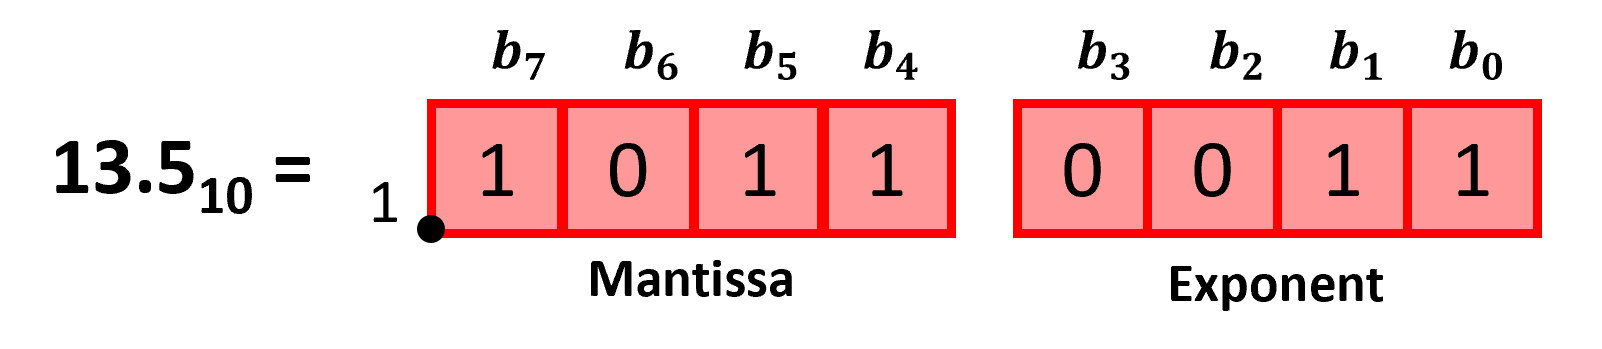
\includegraphics[width= 0.8\textwidth]{./doc/Figures/FloatFloat2.png}
    \caption{Representation of number 13.5 with floating-point format using only 1 byte (8 bits).}
    \label{fig:FloatFloat}
\end{figure}

Since the integer part of the mantissa is always 1, we only need to encode the fractional part.
Given a binary floating point representation with these 8 bits ($b_7, \ldots, b_0$) 
and noticing that $b_3 = 0$ encodes a positive exponent and $b_3 = 1$ a negative exponent, 
the decimal number is obtained by:
$$
   x = m \ 2^e, \quad m =  b_7 \ 2^{-1}  + b_6 \ 2^{-2} + b_5 \ 2^{-3} + b_4 \ 2^{-4}, \quad 
    e =  (-1)^{b_3} (  b_2 \ 2^{2} + b_1 \ 2^{1} + b_0 \ 2^{0} ) 
$$

The maximum value allowed with this representation is: 
$$
   \texttt{1111 0111} = 1.9375 \times 2^{7}
$$   
and the smallest number is: 
$$
   \texttt{0000 1111} =  2^{-7}.
$$ 
In this representation, the distance between the maximum number and its closest number is $2^3$
and the distance between the minimum number and its closest number is $ 2^{-11}$. Hence, in a 
much bigger range we manage variable distances between reals, extremely shorts near 0 and really big 
for bigger values. 





To conclude, for the same number of bits, fixed-point numbers are equal-spaced along 
the whole range but with a smaller range ($31.875$ vs $ 1.9375 \times 2^{7}$).
The distance among real numbers in the fixed-point representation is constant ($0.125$ in our example). 
However, in the floating-point representation, the distance among real numbers 
changes from extremely short values to very big distances ($2^{-11}$ to $ 2^{7}$) depending on the exponent of the real number. 
never forget that the total amount of real numbers in fixed point or floating point 
representation is exactly the same but their distribution and range are different.


\begin{IN}
    \begin{enumerate}
        \item Fixed-point format has constant distance among all representable real numbers and a small range. 
        \item Floating-point format has variable distance among all representable real numbers with a huge range.  
    \end{enumerate}
\end{IN}


In the following section the standard IEEE 754, which is used in all computers, is 
explained in detail to understand how real numbers are stored in floating point representation.


%I change this part

%In order to compare with floating-point representation
%let's consider a mini-float of same size, 8 bits.
%In this case 4 bits are reserved for the exponent (1 for its sign and 3 for its value) 
%and 4 bits for the mantissa. 
%Once again no negative values are encoded.
%
%Since the integer part of the mantissa is always a 1 we just need to encode the fractional part.
%Given a binary floating point representation with these 8 bits ($b_7, \ldots, b_0$), 
%the decimal number is obtained by:
%$$
%x = m \ 2^e, \quad m =  b_7 \ 2^{-1}  + b_6 \ 2^{-2} + b_5 \ 2^{-3} + b_4 \ 2^{-3}, \quad 
%e =  \pm (  b_2 \ 2^{2} + b_1 \ 2^{1} + b_0 \ 2^{0} ) 
%$$
%The maximum value with this representation is: 
%$$
%\texttt{1111 1111} = 15 \times 2^{7}
%$$   
%and the smallest number is: 
%$$
%\texttt{0001 0111} =  2^{-7}.
%$$ 
%The distance between the maximum number and its closest  number is:  $  2^{7}$
%and the distance between the minimum number and its closest number is:  
%$ 2^{-7}.$



%%%%RESTOS

%These are not used in numerical calculations where simple precision (4 bytes) 
%is the smallest precision used. 
%However, it needs from the same amount of memory space 
%as the previous example so it can be a good comparison to understand the concept. 

%Do not worry if the notation is not clear right now, it is explained later for the 4-bytes precision, 
%which is similar. 

% and an exponent bias of +7 
%(these concepts are broaden in this section). 
%This representation allows a range between $r\in (-480 = 1 1111 111_2, 480 = \texttt{0 1111 111}_2)$ 
%and 


% $0.0078125_{10} =_2$. 
%We are not discussing now if the number $0 0000 000_2$ is reserved for the $0$ 
%or the number $\texttt{0 1111 111}$ or $\texttt{1 1111 111}$ are reserved for $\pm\infty$ 
%since this is just an example of the capabilities of floating-point representation. 

%In order to compare with floating-point representation,
%let's consider a mini-float of 8 bits with the same memory size that 
%the above fixed point representation. 
%Consider a mini-float with
%4 bits for the exponent (1 for its sign and 3 for its value) and 4  bits for the mantissa.
%Giving a binary floating point representation with 8 bits ($b_7, \ldots, b_0$), 
%the decimal number is obtained by: 


%There are two main ways to represent real numbers in computers: 
%\begin{itemize}
%    \item Fixed-point representation. 
%The real number is represented by its integer part and its decimal part (e.g. \texttt{55.88}). 
%    \item Floating-point representation. 
% The real number is represented by its mantissa and its exponent  (e.g. \texttt{0.5588e02}).
%\end{itemize} 

%     Fixed-point format actually could represent larger numbers or smaller numbers,
%     but it has a static range, which means that the choose is done when designing the code, 
%     later you can only use that range, 
%     either big or small numbers. 
%     Luckily, floating-point format has dynamic range, 
%     which means that once designed the format it can handle 
%     at the same time large and tiny numbers just varying the exponent. 




    %--------------------------------------------------------------------------------------------------------------------------------------
    \section{Floating-point representation in IEEE 754}


Before delving into the particularities of the representation in the standard IEEE 754 a summary of the main properties is presented here. 
\begin{enumerate}
    \item Similarly to the binary normalized scientific notation, the binary point is located immediately after the first binary digit of the mantissa which is always a 1 (normalized range) and it is not explicitly stored. 
    \item The leftmost digit encodes the sign of the number: 1 for negative number, 0 for positive.
    \item The rightmost digits encode the mantissa. 
    \item Between sign bit and mantissa, the exponent is encoded with an offset-binary representation (using an exponent bias).
\end{enumerate} 

Notice from the table \ref{tab:properties} that the actual bits used in the mantissa is always the number of mantissa bits + 1. 
This is due to an implicit 1 in the left part of binary point, since it is always a 1, is not explicitly stored. 
Hence, the binary mantissa of the example $-110.3125$ is actually $1.10111001010...$ while only the right part of the binary point is stored.
There is one number that can not be written with an implicit 1 in standard scientific notation; 0. 
This is one of the IEEE exceptions that are treated in section \ref{sec:exceptions}. 

The table also shows the range of representable numbers, the minimum and maximum value allowed for each standard format. 

Finally, the information we are usually more interested in; the decimal precision for each format, which is the number of reliable decimal digits. Consider that $log_2(10)\approx 3.32 $ binary digits are needed in order to represent one single decimal digit. 

For example, in single precision the mantissa counts on 24 binary digits (23 explicitly stored and 1 implicit) so: $24/3.32 = 7.2$. 
Enough precision to have 7 decimal digits reliably represented. 
Notice this does not mean that the first 7 digits of the representation equals the expected value, it means that the relative error between both numbers is around $1e-7$. 
Just consider the number $1.3_{10}$, in the standard IEEE 754 in single precision this value is stored as 
$$
\texttt{0 01111111 01001100110011001100110}_2 = 1.2999999523162841796875_{10}
$$
which means that the error caused by the conversion is $-4.76837158203125E-8$ while only the first digit is the same.

\newpage
\begin{figure}
    \centering
    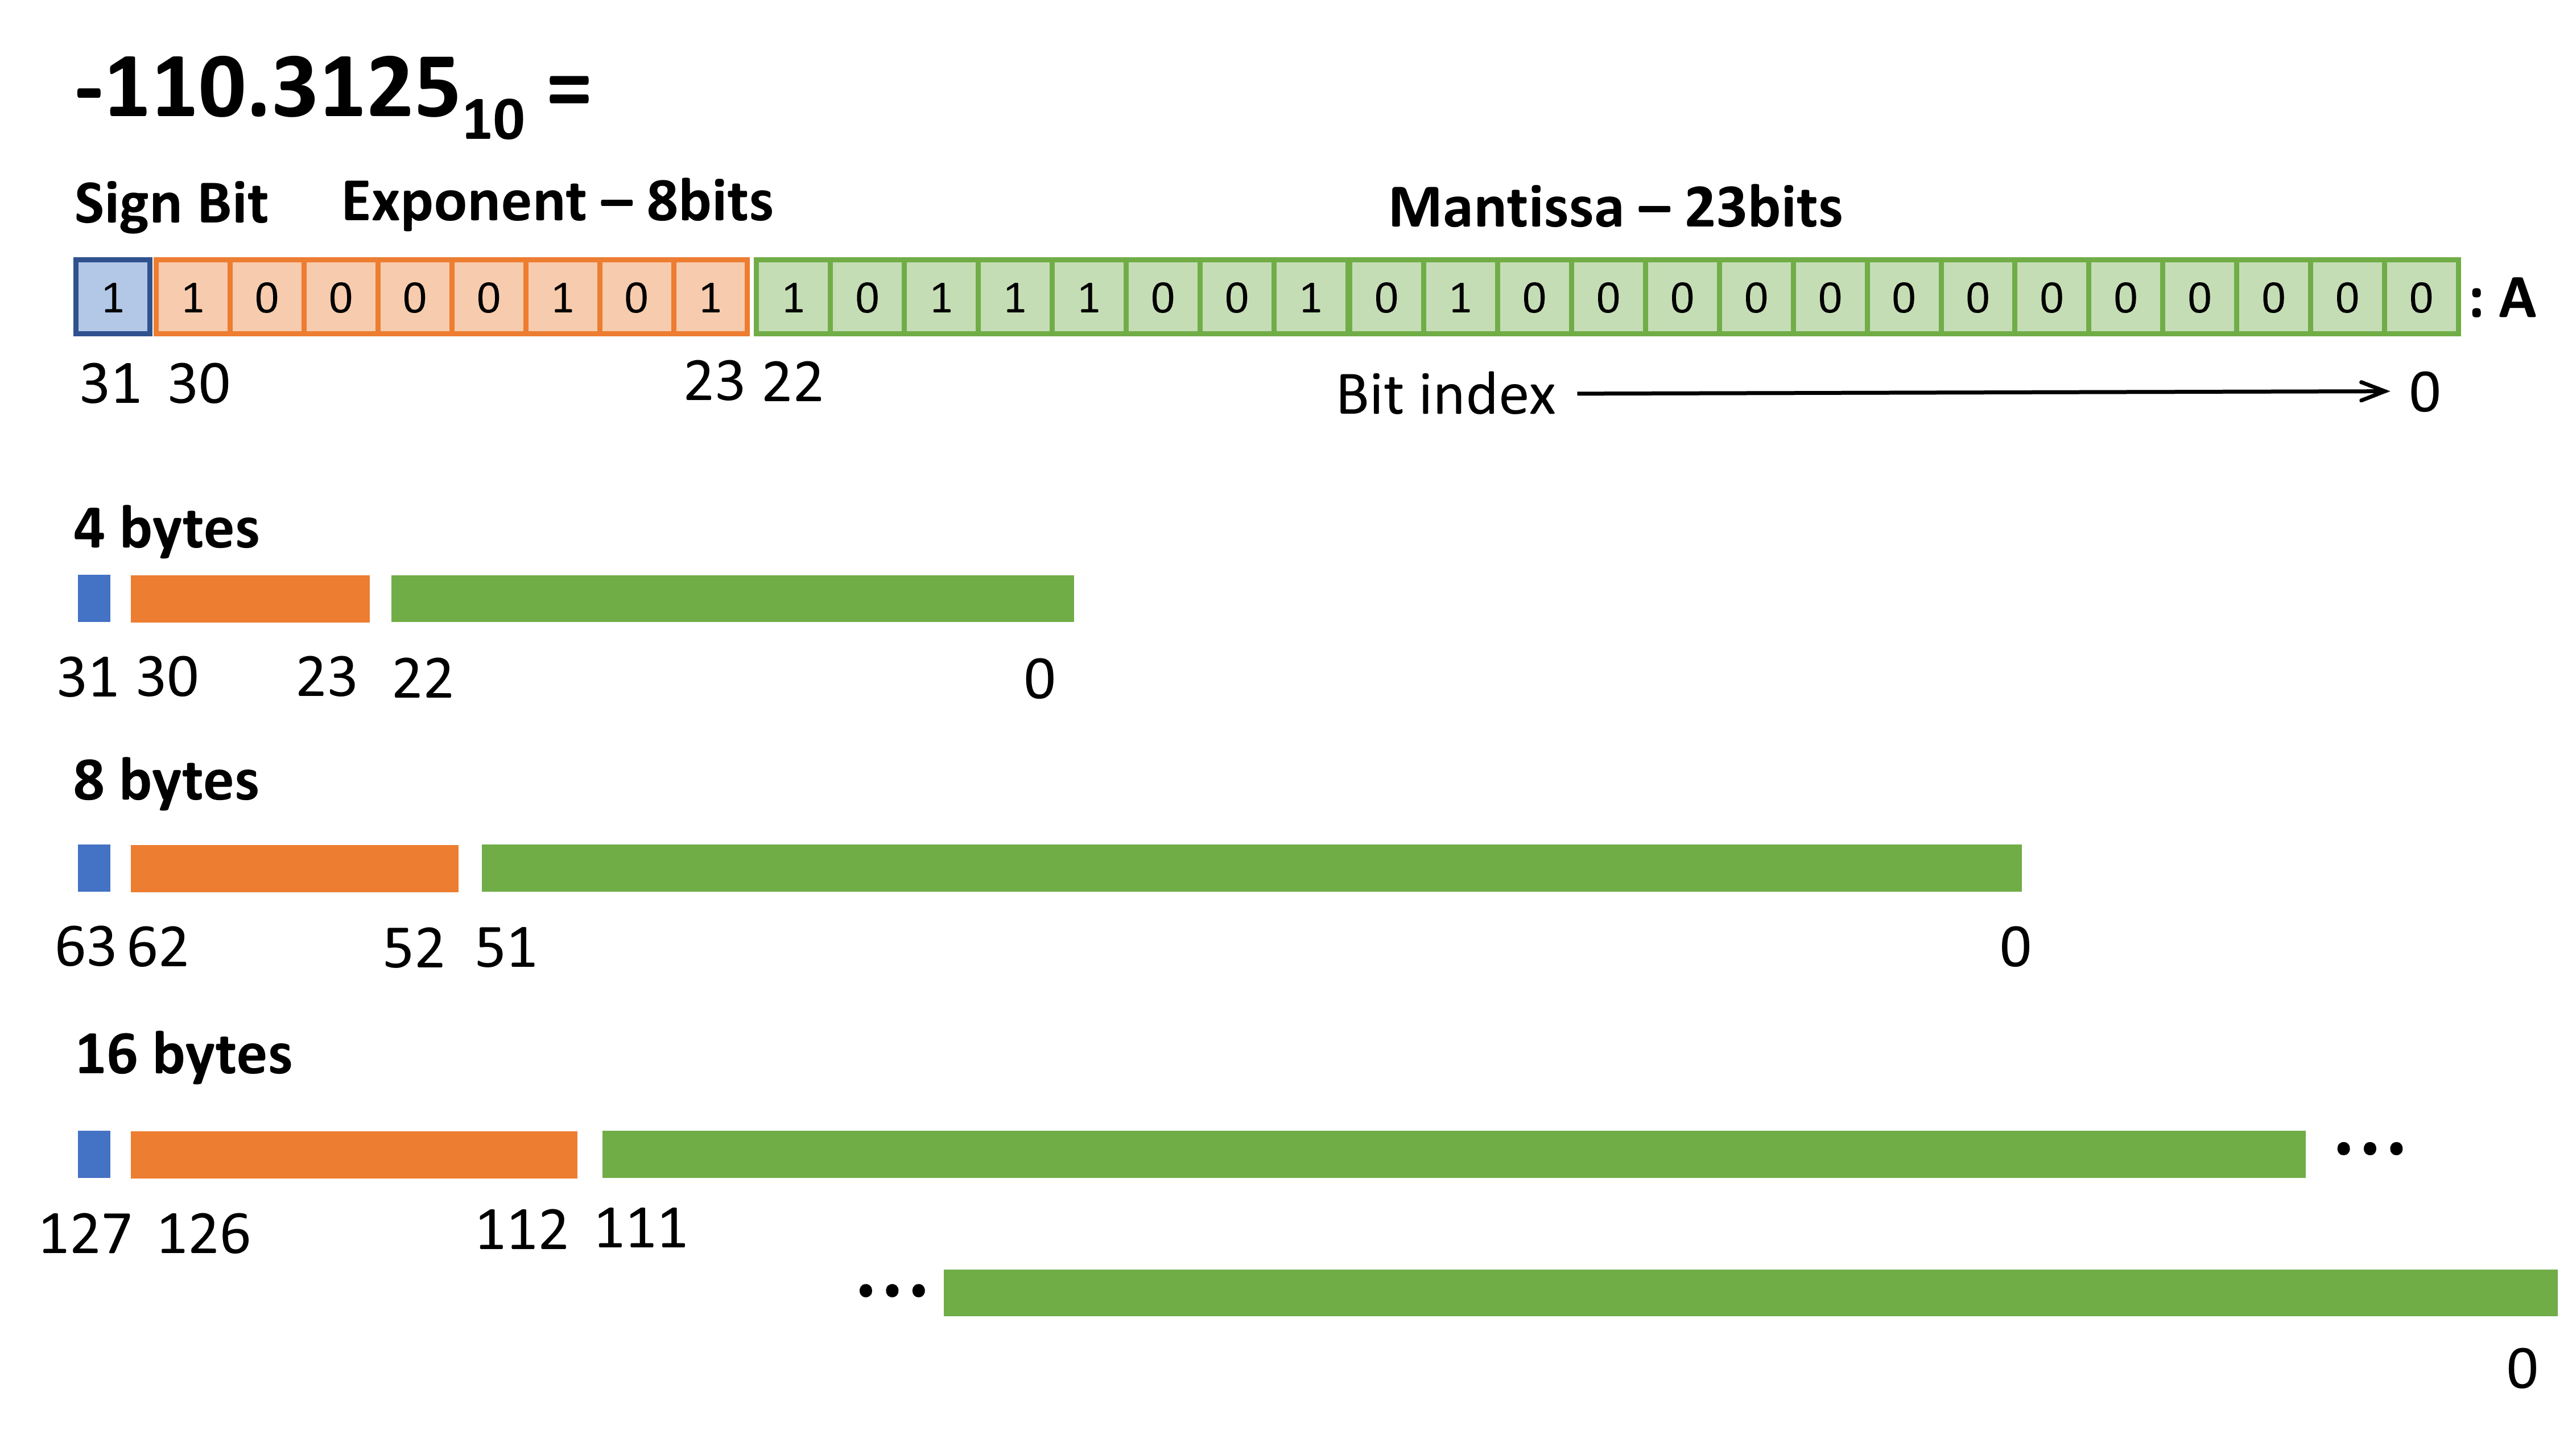
\includegraphics[width= \textwidth]{./doc/Figures/ParametersIEEE.png}
    \caption{Main formats in the standard IEEE 754: single, double and quadruple precision with a visual example in single precision.}
    \label{fig:ParametersIEEE}
\end{figure}
%\begin{table}[H]
%    \centering
%    \begin{tabular}{| r | c | c | c | c | c | }
%        
%        \hline
%        Name & Sign &  \begin{tabular}{@{}c@{}}Exp\\  (r) \end{tabular} &  \begin{tabular}{@{}c@{}}Mantissa\\(p) \end{tabular} & \begin{tabular}{@{}c@{}}Exp. Bias\\  (B) \end{tabular}  & \begin{tabular}{@{}c@{}}Actual Bits\\  mantissa\end{tabular}  \\ \hline
%        
%        \begin{tabular}{@{}c@{}}Single precision \\ (binary32) \end{tabular}      & 1 & 8  & 23    & 127   & 24 \\ \hline
%        
%        \begin{tabular}{@{}c@{}}Double precision \\ (binary64) \end{tabular}    & 1 & 11 & 52    & 1023  & 53   \\  \hline
%        
%        \begin{tabular}{@{}c@{}} Quadruple precision\\(binary128) \end{tabular}   & 1 & 15 & 112   & 16383 & 113   \\ \hline
%        
%    \end{tabular}                                                       
%    %\caption{Main properties of the different precisions covered by the IEEE 754 standard.}
%    %\label{tab:properties}
%\end{table}
%\vspace{-1cm}
%\begin{table}[H]
%    \centering
%    \begin{tabular}{| r | c | c | c |}
%        
%        \hline
%        Name  & \begin{tabular}{@{}c@{}}Normalized \\ range \end{tabular} & \begin{tabular}{@{}c@{}}Approximate\\decimal range\end{tabular} & Precision \\ \hline
%        
%        \begin{tabular}{@{}c@{}}Single precision \\ (binary32) \end{tabular}      &  \begin{tabular}{@{}c@{}}$\pm2^{-126}$ to \\$\pm2^{127+1}$  \end{tabular}    & \begin{tabular}{@{}c@{}}$\pm1.18\cdot10^{ -38}$ to \\ $\pm3.4\cdot10^{38}$ \end{tabular}     & \sim 7 digits  \\ \hline
%        
%        \begin{tabular}{@{}c@{}}Double precision \\ (binary64) \end{tabular}    &  \begin{tabular}{@{}c@{}}  $\pm2^{-1022}$ to\\  $\pm2^{1023+1}$\end{tabular}  & \begin{tabular}{@{}c@{}} $\pm2.23\cdot10^{ -308}$ to \\ $\pm1.80\cdot10^{308}$ \end{tabular} & \sim 15 digits        \\  \hline
%        
%        \begin{tabular}{@{}c@{}} Quadruple precision\\(binary128) \end{tabular}   &  \begin{tabular}{@{}c@{}}  $\pm2^{-16382}$ to\\  $\pm2^{16383+1}$\end{tabular}   & \begin{tabular}{@{}c@{}} $\pm3.3621\cdot 10^{-4932}$ to \\ $\pm1.1897\cdot10^{4932}$ \end{tabular}  & \sim 19 digits          \\ \hline
%        
%    \end{tabular}                                                       
%    \caption{Main properties of the different precisions covered by the IEEE 754 standard.}
%    \label{tab:properties}
%\end{table}

\begin{table}[H]
    \centering
    \begin{tabular}{| r | c | c | c | c | c | }
        
        \hline
        Name & Sign &  \begin{tabular}{@{}c@{}}Exp\\  (r) \end{tabular} &  \begin{tabular}{@{}c@{}}Mantissa\\(p) \end{tabular} & \begin{tabular}{@{}c@{}}Exp. Bias\\  (B) \end{tabular}  & \begin{tabular}{@{}c@{}}Actual Bits\\  mantissa\end{tabular}  \\ \hline
        
        Single precision       & 1 & 8  & 23    & 127   & 24 \\ \hline
        
        Double precision    & 1 & 11 & 52    & 1023  & 53   \\  \hline
        
         Quadruple precision   & 1 & 15 & 112   & 16383 & 113   \\ \hline
        
    \end{tabular}                                                       
    %\caption{Main properties of the different precisions covered by the IEEE 754 standard.}
    %\label{tab:properties}
\end{table}
\begin{table}[H]
    \centering
    \begin{tabular}{| r | c | c | c |}
        
        \hline
        Name  & \begin{tabular}{@{}c@{}}Normalized \\ range \end{tabular} & \begin{tabular}{@{}c@{}}Approximate\\decimal range\end{tabular} & Precision \\ \hline
        
        \begin{tabular}{@{}c@{}}Single precision \\ (binary32) \end{tabular}      &  \begin{tabular}{@{}c@{}}$\pm2^{-126}$ to \\$\pm2^{127+1}$  \end{tabular}    & \begin{tabular}{@{}c@{}}$\pm1.18\cdot10^{ -38}$ to \\ $\pm3.4\cdot10^{38}$ \end{tabular}     & \sim 7 digits  \\ \hline
        
        \begin{tabular}{@{}c@{}}Double precision \\ (binary64) \end{tabular}    &  \begin{tabular}{@{}c@{}}  $\pm2^{-1022}$ to\\  $\pm2^{1023+1}$\end{tabular}  & \begin{tabular}{@{}c@{}} $\pm2.23\cdot10^{ -308}$ to \\ $\pm1.80\cdot10^{308}$ \end{tabular} & \sim 15 digits        \\  \hline
        
        \begin{tabular}{@{}c@{}} Quadruple precision\\(binary128) \end{tabular}   &  \begin{tabular}{@{}c@{}}  $\pm2^{-16382}$ to\\  $\pm2^{16383+1}$\end{tabular}   & \begin{tabular}{@{}c@{}} $\pm3.3621\cdot 10^{-4932}$ to \\ $\pm1.1897\cdot10^{4932}$ \end{tabular}  & \sim 19 digits          \\ \hline
        
    \end{tabular}                                                       
    \caption{Main properties of the different precisions covered by the IEEE 754 standard.}
    \label{tab:properties}
\end{table}








%RESTOS

%\newpage
%%\begin{figure}[h]
%\begin{sidewaysfigure}
%%    %\begin{flushleft}
%%    \centering
%%    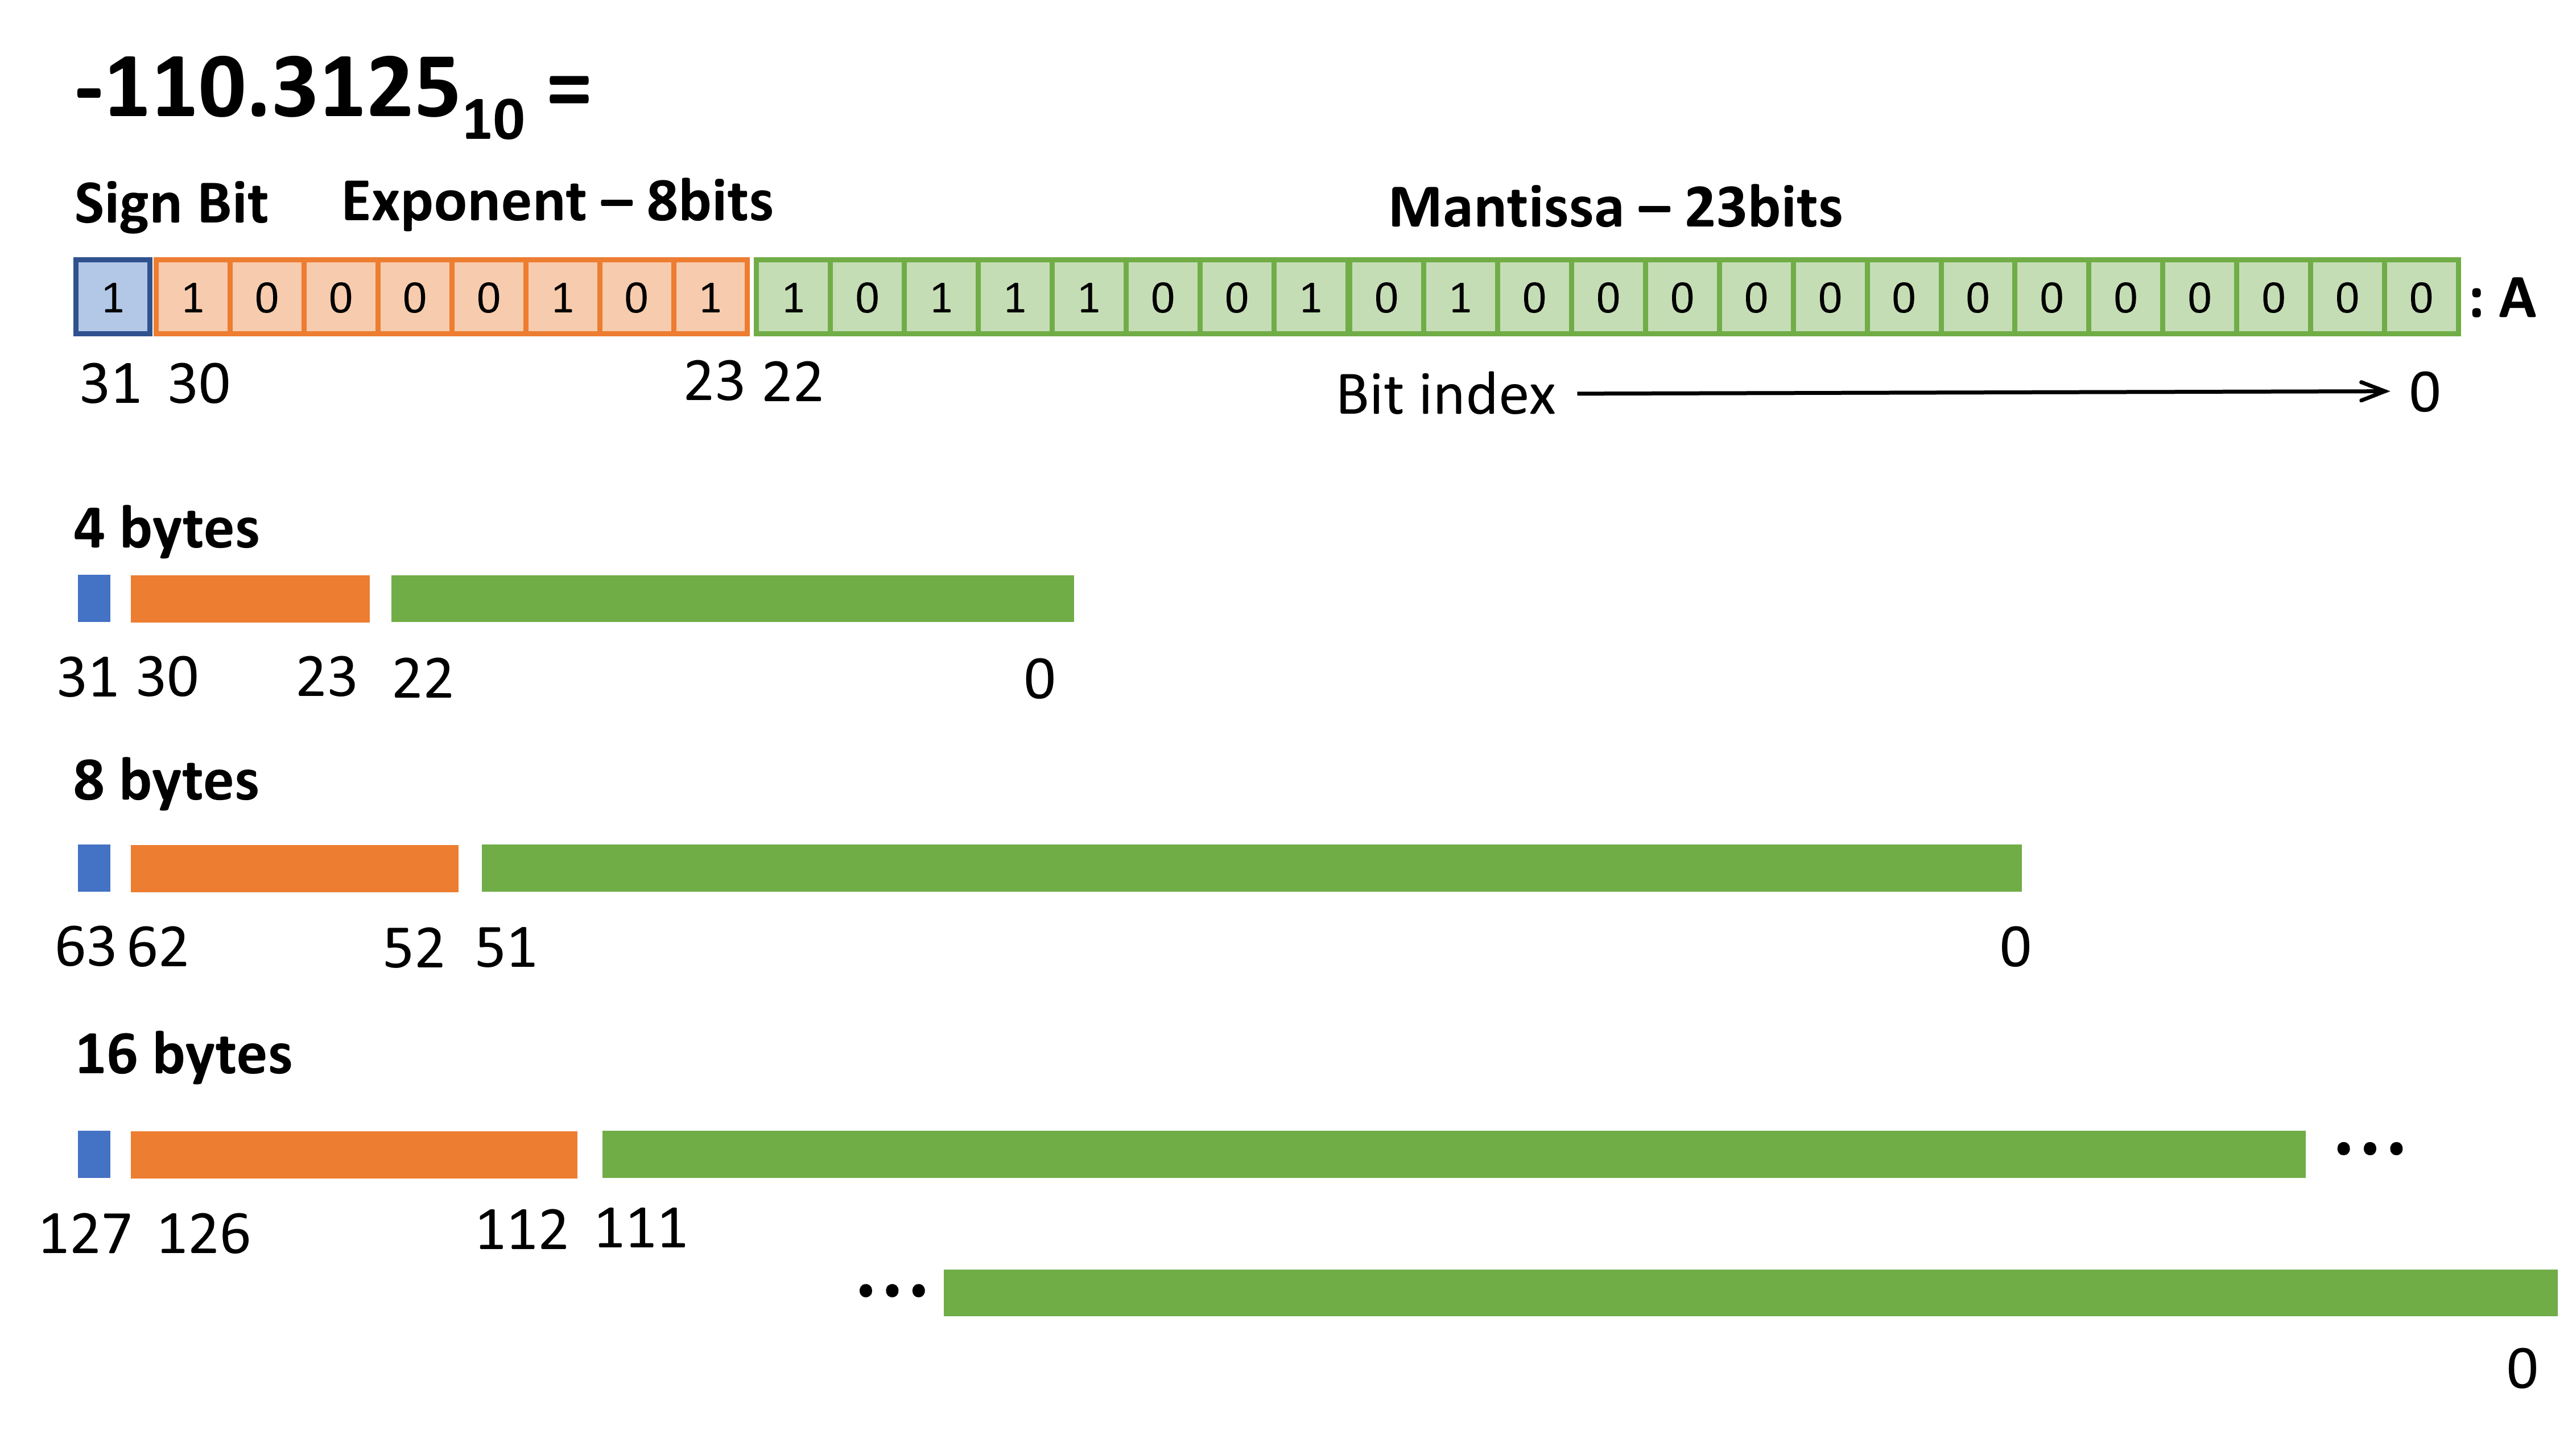
\includegraphics[width= \textwidth]{./doc/Figures/ParametersIEEE.png}
%%    \caption{Main formats in the standard IEEE 754: single, double and quadruple precision with an example in single precision.}
%%    \label{fig:ParametersIEEE}
%%    %\end{flushleft}
%    \begin{table}[H]
%        %\begin{flushright}
%        %\begin{turn}{90}
%        \begin{tabular}{| r | c | c | c | c | c | c | c | c |}
%            
%            \hline
%            Name & Sign & Exp. & Mantissa & Exp. Bias & \begin{tabular}{@{}c@{}}Bits\\  precision\end{tabular}  & \begin{tabular}{@{}c@{}}Normalized \\ range \end{tabular} & \begin{tabular}{@{}c@{}}Approximate\\decimal\end{tabular} & Precision \\ \hline
%            
%            \begin{tabular}{@{}c@{}}Single precision \\ (binary32) \end{tabular}      & 1 & 8  & 23    & +127   & 24 & \begin{tabular}{@{}c@{}}$\pm2^{-126}$ to \\$\pm2^{127+1}$  \end{tabular}    & \begin{tabular}{@{}c@{}}$\pm1.18\cdot10^{ −38}$ to \\ $\pm3.4\cdot10^{38}$ \end{tabular}     & \sim 7.2 digits  \\ \hline
%            
%            \begin{tabular}{@{}c@{}}Double precision \\ (binary64) \end{tabular}    & 1 & 11 & 52    & +1023  & 53 & \begin{tabular}{@{}c@{}}  $\pm2^{-1022}$ to\\  $\pm2^{1023+1}$\end{tabular}  & \begin{tabular}{@{}c@{}} $\pm2.23\cdot10^{ −308}$ to \\ $\pm1.80\cdot10^{308}$ \end{tabular} & \sim 15.9 digits        \\  \hline
%            
%            \begin{tabular}{@{}c@{}} Quadruple precision\\(binary128) \end{tabular}   & 1 & 15 & 112   & +16383 & 113 & \begin{tabular}{@{}c@{}}  $\pm2^{-16382}$ to\\  $\pm2^{16383+1}$\end{tabular}   & \begin{tabular}{@{}c@{}} $\pm3.3621\cdot 10^{-4932}$ to \\ $\pm1.1897\cdot10^{4932}$ \end{tabular}  & \sim 19.2 digits          \\ \hline
%            
%        \end{tabular}                                                       
%        %\end{turn}
%        \caption{Main properties of the different precisions covered by the IEEE 754 standard.}
%        \label{tab:properties}
%        %\end{flushright}
%    \end{table}
%\end{sidewaysfigure}
%%\end{figure}








    %--------------------------------------------------------------------------------------------------------------------------------------
    \newpage 
    \FloatBarrier
    \section{Distance between floating-point real numbers} \label{sec:roundoff}


        %-------------------------------------------------------------------------------------------------------------------------------------- 
        \subsection{Floating-point distribution in the numbers line}

In this section we delve into the relation between the amount of bits reserved to store exponent-mantissa and 
the density of floating-point values in the numbers line. 
Let's consider a vastly simplified format of only 4 bits: $2$ binary digits for the mantissa $p = 2$ (using an implicit 1) and 
$2$ digits for the exponent (four available exponents: $-1, 0, 1, 2$). In addition, not sign bit is considered (see Figure \ref{fig:miniminifloat}).

\begin{minipage}{\textwidth}
    \begin{minipage}{0.3\textwidth}
        \centering
        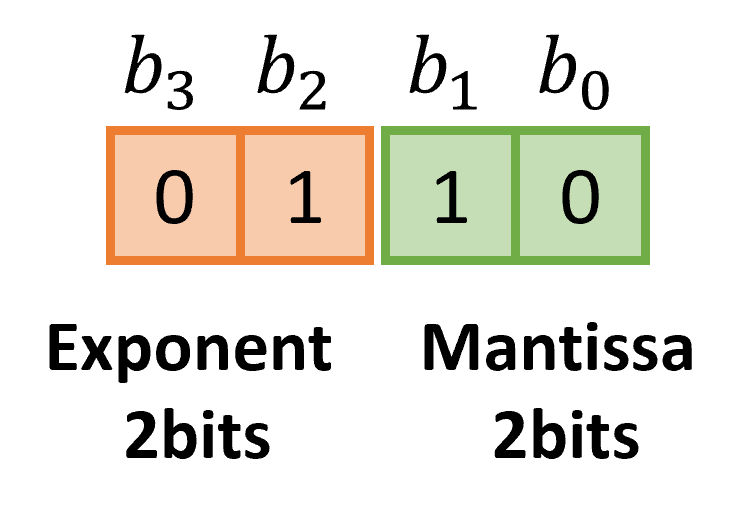
\includegraphics[width= \textwidth]{./doc/Figures/miniminifloat.png}
        \captionof{figure}{Simplified floating-point representation with only 4 bits.}
        \label{fig:miniminifloat}
    \end{minipage}
    \hfill
    \begin{minipage}{0.68\textwidth}
        \centering
        \begin{tabular}{| c | c | c | c | c | }
            \hline
            Mantissa/Exponent   & $-1$ & $0$  & $1$  &   $2$  \\ \hline
            1.00                & $0.5$ & $1$  & $2$  &   $4$  \\ \hline
            1.01                & $0.625$ & $1.25$  & $2.5$  &   $5$  \\ \hline
            1.10                & $0.75$ & $1.5$  & $3$  &   $6$  \\ \hline
            1.11                & $0.875$ & $1.75$  & $3.5$  &   $7$  \\ \hline
        \end{tabular}
        \captionof{table}{Possible decimal values covered by the example system treated.}
        \label{tab:PossibleValues}
    \end{minipage}
\end{minipage}

A general floating-point number in this system is written (see \cite{articleIEEE}): 
$$
1.dd \times 2^{e}    \quad \textrm{with}\quad e \in \mathbb{Z}, e\in\left[-1, 2\right] 
$$ 
A maximum of $2^4 = 16$ values can be represented with this system. 
The possible values, those reals that has exact representation in this system,
are written in the table \ref{tab:PossibleValues} and
plotted in the numbers line of the Figure \ref{fig:DensityNumbers}. 

\begin{figure}[h]
    \centering
    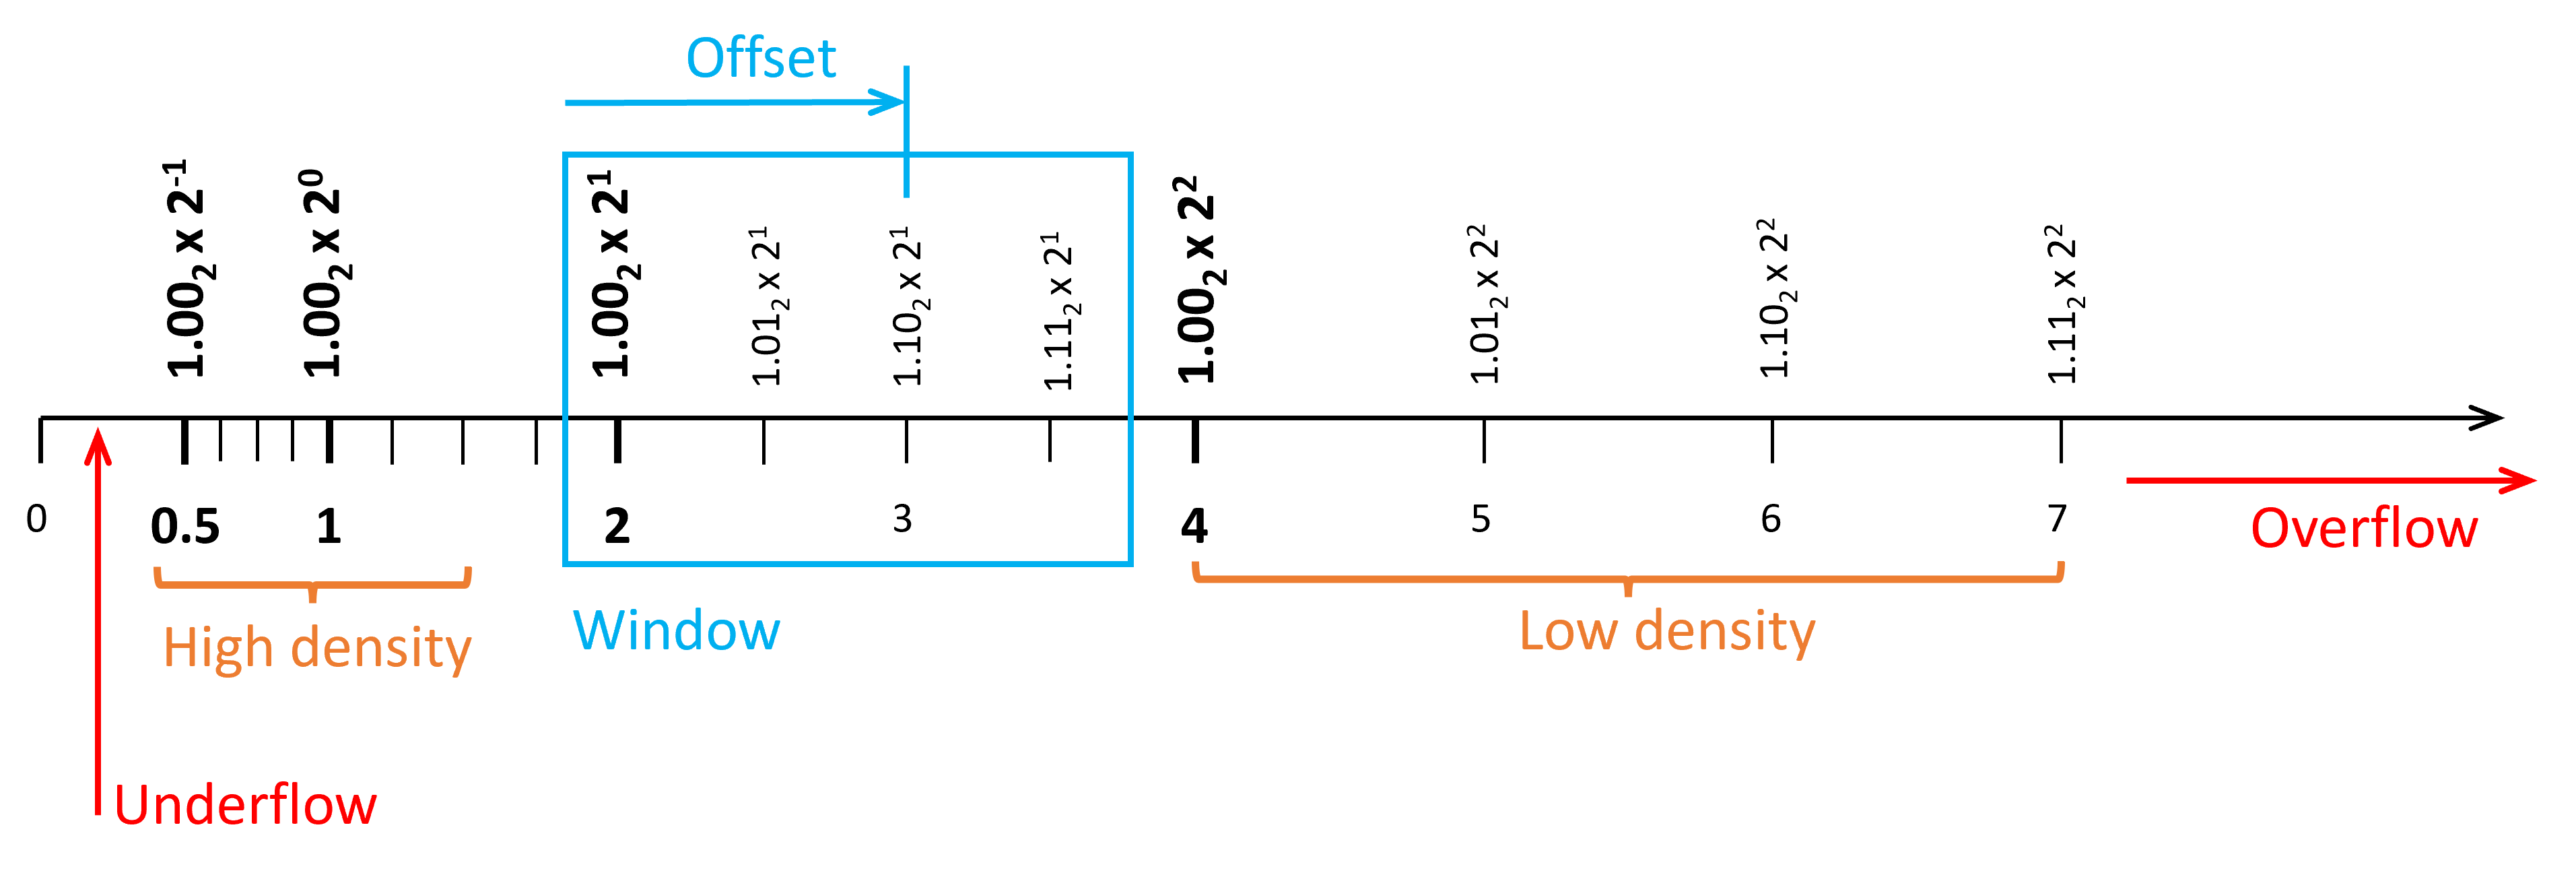
\includegraphics[width= \textwidth]{./doc/Figures/DensityNumbers.png}
    \caption{Representation of the possible values covered by the example system treated.}
    \label{fig:DensityNumbers}
\end{figure}




\FloatBarrier
Think of the exponent as a window between two values 
and the mantissa as the offset of every number inside that window (see \cite{VisExpl}).
In the decimal system a window is limited by two consecutive powers-of-ten: [0.1,1], [1,10], [10,100], etc. 
In binary each window is bounded by powers-of-two: [0.5,1], [1,2], [2,4], etc. 

The exponent of a number fixes its window. Then, 
every window is equidistantly divided according to the number of bits used for the mantissa. 
Both the least significant bit in the mantissa and the exponent tell us the constant distance between values in that window. 

Notice that from one window to the next the number of divisions is the same but the length of the window is twice the previous.
Hence, the resolution in that window is lower and the programmer is loosing capacity to represent numbers. 
Said in other words, the density of floating-point values near the zero is bigger than 
the density of values with growing values. 





%-----------------------------------
It is difficult to represent the density of representable numbers in the numbers line for IEEE 754 standard formats.
However, the behaviour is exactly the same, but with much more values.
Consider a single precision mantissa. 
We count on 23 binary digits to divide every window: $2^{23} = 8688608$ possible values. 

In the window $\left[1,2\right]$ (exponent $0$) the resolution is:
$$
\frac{\left(2-1\right)}{2^{23}} \simeq 0.000000119
$$ 
while in the window $\left[32768=2^{15},65536=2^{16}\right]$ the resolution is:
$$
\frac{\left(65536-32768\right)}{2^{23}} \simeq 0.003906
$$
To conclude, the density of numbers that are exactly represented in IEEE 754 decreases 
when we move away from 0 on the numbers line. 
%-----------------------------------





%RESTOS
%\begin{figure}[H]
%    \centering
%    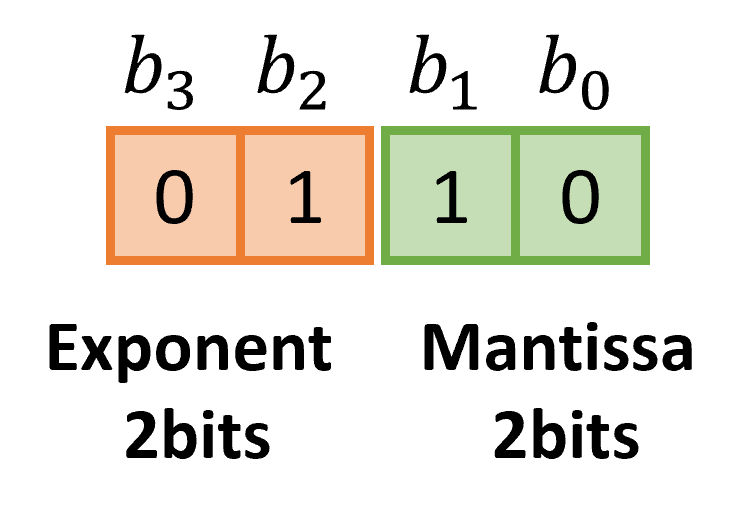
\includegraphics[width= .3\textwidth]{./doc/Figures/miniminifloat.png}
%    \caption{Simplified floating-point representation with only 4 bits.}
%    \label{fig:miniminifloat}
%\end{figure}

%\begin{table}
%    \centering
%    \begin{tabular}{| c | c | c | c | c | }
%        \hline
%        Mantissa/Exponent   & $-1$ & $0$  & $1$  &   $2$  \\ \hline
%        1.00                & $0.5$ & $1$  & $2$  &   $4$  \\ \hline
%        1.01                & $0.625$ & $1.25$  & $2.5$  &   $5$  \\ \hline
%        1.10                & $0.75$ & $1.5$  & $3$  &   $6$  \\ \hline
%        1.11                & $0.875$ & $1.75$  & $3.5$  &   $7$  \\ \hline
%    \end{tabular}
%    \caption{Possible decimal values covered by the example system treated.}
%    \label{tab:PossibleValues}
%\end{table}


        %-------------------------------------------------------------------------------------------------------------------------------------- 
        \subsection{Absolute and relative error}


The question that arises at this point is: Which is the round-off error when using finite precision floating-point reals?

%-----------------------------------
Let's see an example using the 4-bits system explained in the previous section. Imagine that you need to use the constant: 
$$
3.1875_{10} = 11.0011_2 = 1.10011\times 2^1_2
$$
This number does not have exact representation as we can check in Table \ref{tab:PossibleValues}. It will be rounded to the nearest representable number, which is: 
$$
1.10\times2^1_2 = 3_{10}
$$
The round-off error is $3.1875_{10} - 3_{10} = 0.1875_{10} = 0.0011_2$.
 
Notice that the last representable binary place for the number $1.10\times2^1_2$ is $0.01\times2^1 = 0.1_2$ 
so the error made in our approximation can also be expressed as $0.011_2$ units in the last place (\textit{ulps} $= 2^{e-p}$). 
%-----------------------------------



{\Large Absolute Error}

For a given value $z$ and its representation in a floating-point system $z_{fl}$, 
the absolute error made is the distance between them:
$$
E_{abs} = \abs{z - z_{fl}} 
$$
This error can be expressed by the distance itself or using ulp.

The absolute error for our theoretical 4-bits system is plotted in Figure \ref{fig:AbsErrorGraph}.
\begin{figure}[h]
    \centering
    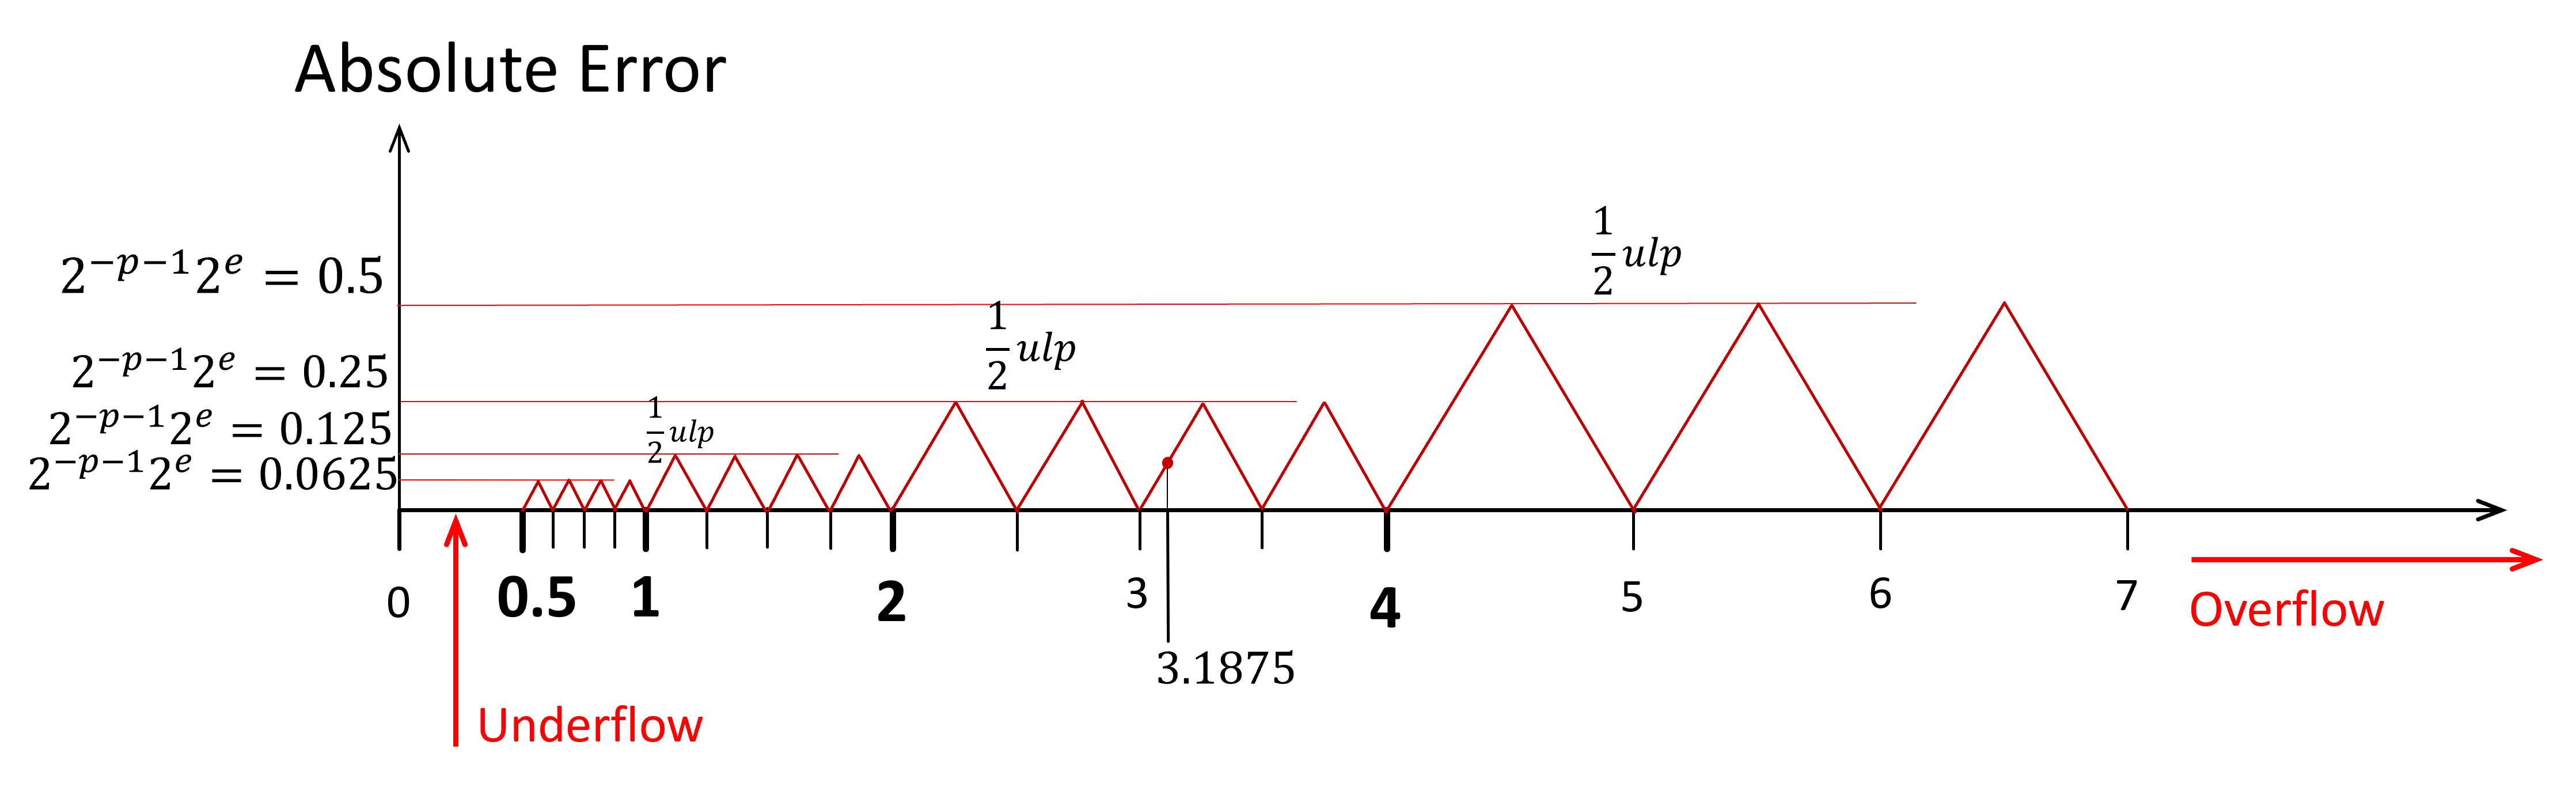
\includegraphics[width= \textwidth]{./doc/Figures/AbsErrorGraph.png}
    \caption{Absolute error made when the reals are approximated by the nearest floating-point value. Notice that reals are attracted by the floating-point values which act as a magnetic grid.}
    \label{fig:AbsErrorGraph}
\end{figure}

Notice that when the exact number is approximated by the nearest floating-point value 
this error is always \textbf{bounded} by half ulp ($0.5_{10}$ ulp $= 0.1_2$ ulp). 
Expressed with ulp seems that this bound is small but remember that the concept \textit{ulp} depends both on 
the binary \textbf{digits of the mantissa} and the \textbf{exponent of the represented number}.
Half ulp is much more important if we are representing a number around $2^{24}$ than a number near $2^1$.





{\Large Relative Error}


Another way to measure the error made in the representation is using the relative error:
$$
E_{rel} = \abs{\frac{z - z_{fl}}{z}} = \abs{1 - \frac{z_{fl}}{z}}
$$
Now, the difference between exact and approximated number is divided by the exact value so
the error does not grow while moving along the numbers line, 
it remains bounded for the whole range. 

The relative error for our theoretical 4-bits system is plotted in Figure \ref{fig:RelErrorGraph}.
\begin{figure}[h]
    \centering
    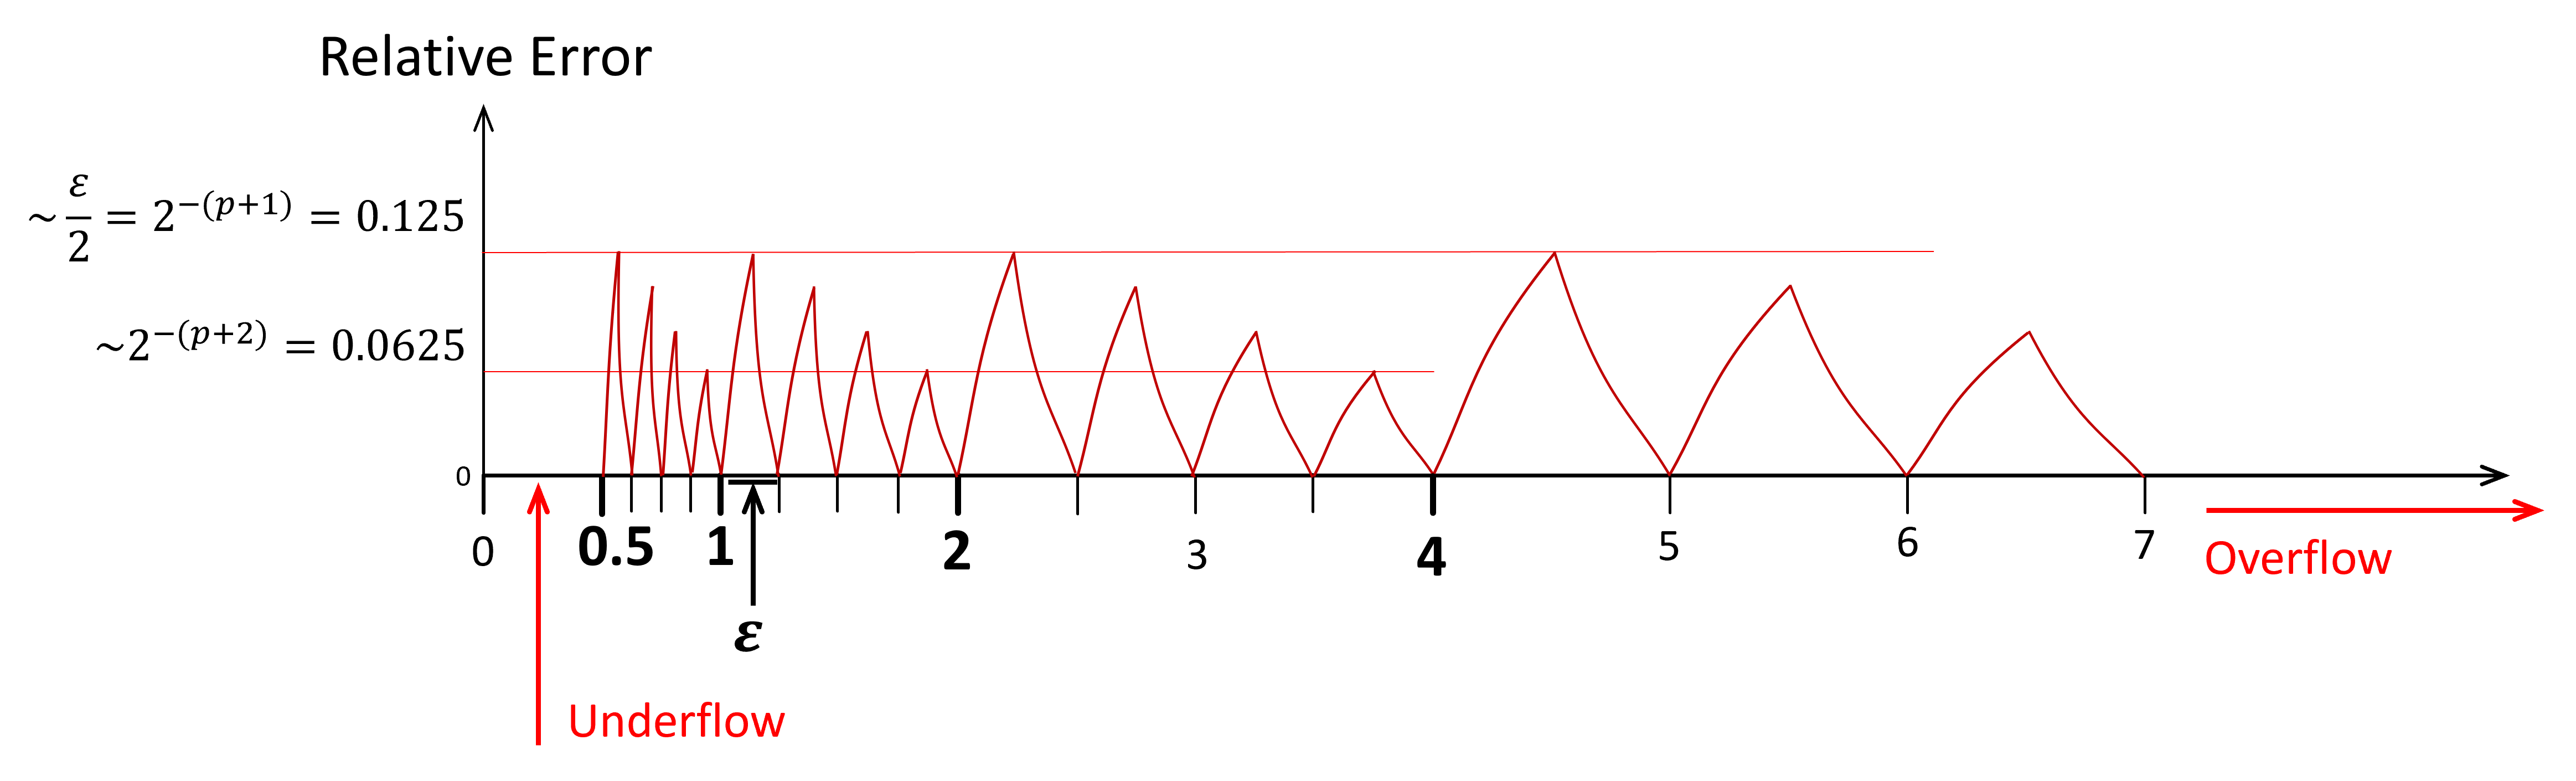
\includegraphics[width= \textwidth]{./doc/Figures/RelErrorGraph.png}
    \caption{Relative error made when the reals are approximated by the nearest floating-point value.}
    \label{fig:RelErrorGraph}
\end{figure}

When the exact number is approximated by the nearest floating-point value we can also find an expression 
for the bounds of this error. Let's find the relative error associated to the maximums of the absolute error made in any window.
For every window (exponent) $z$ varies in the range 
$$
z \in \left[2^e, 2\times 2^e\right)
$$ 
and the maximum absolute error in that window is $\frac{1}{2}\textrm{ulp} = 2^{e-p-1}$.
Then, the maximums of the relative error ranges in:
$$
\left[\frac{2^{e-p-1}}{2^{e+1}},  \frac{2^{e-p-1}}{2^e} \right] = \left[2^{-(p+2)},  2^{-(p+1)} \right]
$$
The highest value of the different peaks happens around the beginning of the window, 
when the value of $z$ is lower (see Figure \ref{fig:RelErrorGraph}). 







This example imitates perfectly what happen with IEEE 754 floating-point formats. Both errors behave in the same way but with different values. 
The table \ref{tab:errors} shows these magnitudes generalised for any binary floating-point format where 
$p$ is the number of digits reserved for the mantissa and $e$ is the exponent of the value $z$ to be represented.
\begin{table}
    \centering
    \begin{tabular}{| c | l | }
        \hline
        \textbf{Definition}       & \textbf{Expression}  \\ \hline %%%%%%
        ulp                       & $2^{e-p} = 0.0000...01 \times 2^e $  \\ \hline
        Absolute error of $z$     & $ \abs{z - z_{fl}} = \abs{z - 1.dddd...\times 2^e} $ \\ \hline   %%%%%%%
        \begin{tabular}{@{}c@{}} Max absolute error   \\    for a given exponent    \end{tabular}    & $ \frac{1}{2} ulp = 2^{e-p-1}$  \\ \hline   %%%%%%%
        Relative error            & $ \abs{\frac{z - z_{fl}}{z}} = \abs{1 - \frac{z_{fl}}{z}} = \abs{\frac{z - 1.dddd...\times 2^e}{z}}$  \\ \hline
        Bounds for relative error   & $\left[2^{-(p+2)}, 2^{-(p+1)} \right]$   \\ \hline     %%%%%%%
    \end{tabular}
    \caption{Main magnitudes that describe the representation of a value $z$ in a floating-point binary format when it is approximated by the nearest floating-point value $z_{fl}$.}
    \label{tab:errors}
\end{table}

When a variable is initialized or a constant value defined, the exact value is approximated by the nearest IEEE 754 number. Then, we have seen that the absolute error is bounded. 
On the contrary, when operating (adding, multiplying, dividing, etc.) with reals, the finite precision result of the operation could be different from the nearest IEEE value to the exact result.
The absolute error, whether expressed in units or with ulps, is usually used to understand the rounding error along the numbers line. However, the relative error is better to analyse calculations.  

\begin{IN}
    \begin{itemize}
        \item The term \textit{ulp} is used to indicate the last representable binary place for a floating point, it depends on the number of mantissa digits and the exponent of the number to be represented: $ulp = 2^{e-p}$. 
        \item The absolute round-off error grows with the exponent but always bounded by $\frac{1}{2} ulp = 2^{e-p-1}$.
        \item The relative round-off error is bounded by a constant value along the numbers line equal to $2^{-(p+1)}$.
    \end{itemize}   
\end{IN} 




%\begin{IN}
%    \begin{itemize}
%        \item Use the absolute error, whether expressed in units or with ulps, to understand the rounding error along the numbers line. 
%        \item Use the relative error to analyse the results of your calculations in the computer.
%    \end{itemize}   
%\end{IN}  



%RESTOS
%which in our example system is:
%$$
%E_{abs} =  \abs{z - 1.dd\times 2^e} = \abs{ \left(  \frac{z}{2^e}  \right) - 1.dd }2^e
%$$

%\begin{table}
%    \centering
%    \begin{tabular}{| c | l | }
%        \hline
%        \textbf{Definition}       & \textbf{Expression}  \\ \hline %%%%%%
%        ulp                       & $2^{e-p} = 0.0000...1 \times 2^e $  \\ \hline
%        Absolute error of $z$     & $ \abs{d.dddd...\times 2^e - z} = \abs{d.dddd...-\frac{z}{2^e}} 2^e $ \\ \hline   %%%%%%%
%        Maximum absolute error    & $\frac{2^{-p}2^e}{2} = \frac{1}{2} ulp$  \\ \hline   %%%%%%%
%        Relative error            & $\abs{\frac{z - d.dddd...\times 2^e}{z}}$  \\ \hline
%        \begin{tabular}{@{}c@{}} Relative error of the   \\    maximum absolute error    \end{tabular}  & 
%        $\left[2^{-(p+2)}, 2^{-(p+1)} \right]$   \\ \hline     %%%%%%%
%    \end{tabular}
%    \caption{Different errors committed when the real number $z$ is approximated by the nearest floating-point value. Remember that here $p$ is the number of bits of the mantissa excluding the implicit 1. }
%    \label{tab:errors}
%\end{table}


        %--------------------------------------------------------------------------------------------------------------------------------------
        \FloatBarrier
        \subsection{Machine epsilon}

The importance of machine epsilon lies in the fact that this magnitude bounds the 
relative error of any number when is rounded to the closest floating-point value. 
Different definitions are used, however, we consider the following: 
it is the smallest number $\epsilon$ such that $1 + \epsilon > 1$. 
In other words, the distance between 1 and the next larger floating point number (see Figure \ref{fig:RelErrorGraph}).

Machine epsilon is then the smallest change we can make to the number 1 and is obtained by adding one to the least significant bit of the mantissa. 
Hence, calling $p$ to the number of significant digits of the mantissa not including the implicit 1 (see Table \ref{tab:eps}):
$$
\epsilon = 2^{-p}
$$ 

\textit{Notice that sometimes $p$ is used for the mantissa digits including the implicit 1 so a slightly different expression of this machine epsilon can be found.}

Formally, when the exact value to be represented is rounded to the nearest floating-point value, 
the relative error is not bounded by $\epsilon$ but $\frac{\epsilon}{2}$ which is called \textit{unit roundoff}:
$$
\frac{\epsilon}{2} = 2^{-p-1}
$$


\begin{table}[H]
    \centering
    \begin{tabular}{| r | c | c | c | }
        
        \hline
        Name  &  Mantissa (p) & $\epsilon$ & $\frac{\epsilon}{2}$  \\ \hline
        
        \begin{tabular}{@{}c@{}}Single precision \\ (binary32) \end{tabular}     &  23    & $\sim 1.19\cdot10^{-7} $   & $\sim 5.96\cdot10^{-8} $ \\ \hline
        
        \begin{tabular}{@{}c@{}}Double precision \\ (binary64) \end{tabular}    &  52    & $\sim 2.22\cdot10^{-16} $  & $\sim 1.11\cdot10^{-16} $   \\  \hline
        
        \begin{tabular}{@{}c@{}} Quadruple precision\\(binary128) \end{tabular}  & 112   & $\sim 1.93\cdot10^{-34}  $  & $\sim 9.63\cdot10^{-35} $   \\ \hline
        
    \end{tabular}                                                       
    \caption{Bounds of the relative error for the different formats covered by the IEEE 754 standard.}
    \label{tab:eps}
\end{table}



It can be concluded from this chapter that the density of numbers that can be represented near 0 is enormous and this density decreases as 
we move away from 0. A scientific programmer can take advantage of this property and normalize the operations to perform. 
For example, consider an ODE solution where the whole equation is dimensionless with all the terms divided by the 
maximum values that the variables are going to reach. The solution varies around 1, where the IEEE 754 floating point 
set is more dense and the absolute error is lower. 




        %--------------------------------------------------------------------------------------------------------------------------------------
        \subsection{Are integer numbers exactly represented in the reals?}


Integer values in the field of reals follow the same treatment as any other real number so they will be exactly represented with the same number of decimal digits. 
Hence, not all the integers contained in the representable range of real numbers have exact representation in this set. 

In the case of single precision for example, at least all the integers with 6 or less significant decimal digits can be converted to a IEEE 754 value without losing precision. 
Some integers with 9 digits can also be converted but more than 9 digits is inevitably related to loss of precision. 

As an example, the following number is exactly stored: 
$$
899565_{10} = \texttt{0 10010010 10110111001111011010000}
$$
but the number $45962178_{10}$ is converted (with an error of $-2$ units) to:
$$
45962176_{10} = \texttt{0 10011000 01011110101010011110000}
$$



%RESTOS
%There are two reasons why a real number you may want to represent in the computer can not be 
%exactly represented and has to be rounded to an IEEE floating-point value. 
%The first and the less common, the number is out of the 
%representable range either for an overflow or an underflow.
%The second; there is not binary representation for that number, maybe its binary translation has infinite number of 
%digits or maybe it has more significant digits than the allowed by the format used (precision, see 
%\cite{articleIEEE}). 


%RESTOS GENERICOS USANDO beta 

%Let's also find bounds for the relative error, for example, the relative error of the maximum absolute error committed in any window. 
%In this case, for every exponent, the 
%real number varies in the range $z \in \left[\beta^e, \beta \beta^e\right)$ while the maximum absolute error is constant 
%$\frac{1}{2}\textrm{ulp}$ so the relative error ranges in: $\left[\frac{\beta}{2}\beta^{-p}, \frac{1}{2}\beta^{-p} \right]$
%
%\begin{IN}
%    Use the absolute error, whether expressed absolutely or with ulps, to understand the rounding error and use the relative error to analyse 
%    the results of calculations in the computer.
%\end{IN}  
%
%For a general number system where $\beta$ is the base of the system, $p$ is the number of digits reserved for the mantissa and $e$ is the 
%exponent, the table \ref{tab:errors} shows the errors and their bounds. Notice that the definition of the ulp is composed by a part that 
%depends number system ($\beta$ and $p$) and another part that depends on the specific exponent that is represented (the window), $e$. 
%
%\begin{table}
%    \centering
%    \begin{tabular}{| c | l | }
%        \hline
%        \textbf{Definition}   & \textbf{Expression }  \\ \hline
%        ulp                & $\beta\beta^{-p}\beta^e = 0.0000...\beta' \textrm{x} \beta^e    \quad     \textrm{with} \quad \beta' = 
%        \frac{\beta}{2} \textrm{digits}$  \\ \hline
%        Absolute error of $z$             & $\abs{d.dddd...\textrm{x} \beta^e - z} = \abs{d.dddd...-\frac{z}{\beta^e}}\beta^e$ \\ \hline
%        Maximum absolute error            & $\left[\left(\frac{\beta}{2}\right)\beta^{-p}\right]\beta^e = \frac{1}{2} ulp$  \\ \hline
%        Relative error                & $\abs{\frac{z - d.dddd...\textrm{x} \beta^e}{z}}$  \\ \hline
%        \begin{tabular}{@{}c@{}} Relative error of the   \\    maximum absolute error    \end{tabular}           & 
%        $\left[\frac{1}{2}\beta^{-p}, \frac{\beta}{2}\beta^{-p} \right]$   \\ \hline
%    \end{tabular}
%    \caption{Different errors committed when the real number $z$ is approximated by the nearest floating-point value.}
%    \label{tab:errors}
%\end{table}
%
%A good way to understand the expressions and behaviour of these errors is to represented them in the same number line shown above, using that 
%representation system. Because of the high density of the representable number in the IEEE-754 system for simple precision, in that case only 
%the boundaries of the errors are represented, while in the simpler case of only 3 significant digits, is possible to show the exact error for 
%every real number (see Figure \ref{fig:AbsErrorGraph}).
%
%For the relative error, take into account that the each number has its own value, exactly like the absolute error. However, we are more 
%interested in the general behaviour of this error. Since it is calculated dividing the absolute error for the real number ($z$) notice that 
%for each window the relative error is smaller in the higher values (in the right part of the window) while it is higher in the left part. 
%Furthermore, the relative error is exactly the same for all the windows (it does not vary with the exponent of the number represented). Said 
%that, the relative error is always bounded by $\frac{\beta}{2}\beta^{-p}$ in the left part of each window and by $ \frac{1}{2}\beta^{-p} $ in 
%the right part (see Figure \ref{fig:RelErrorGraph}). 
%
%\begin{figure}[h]
%    \centering
%    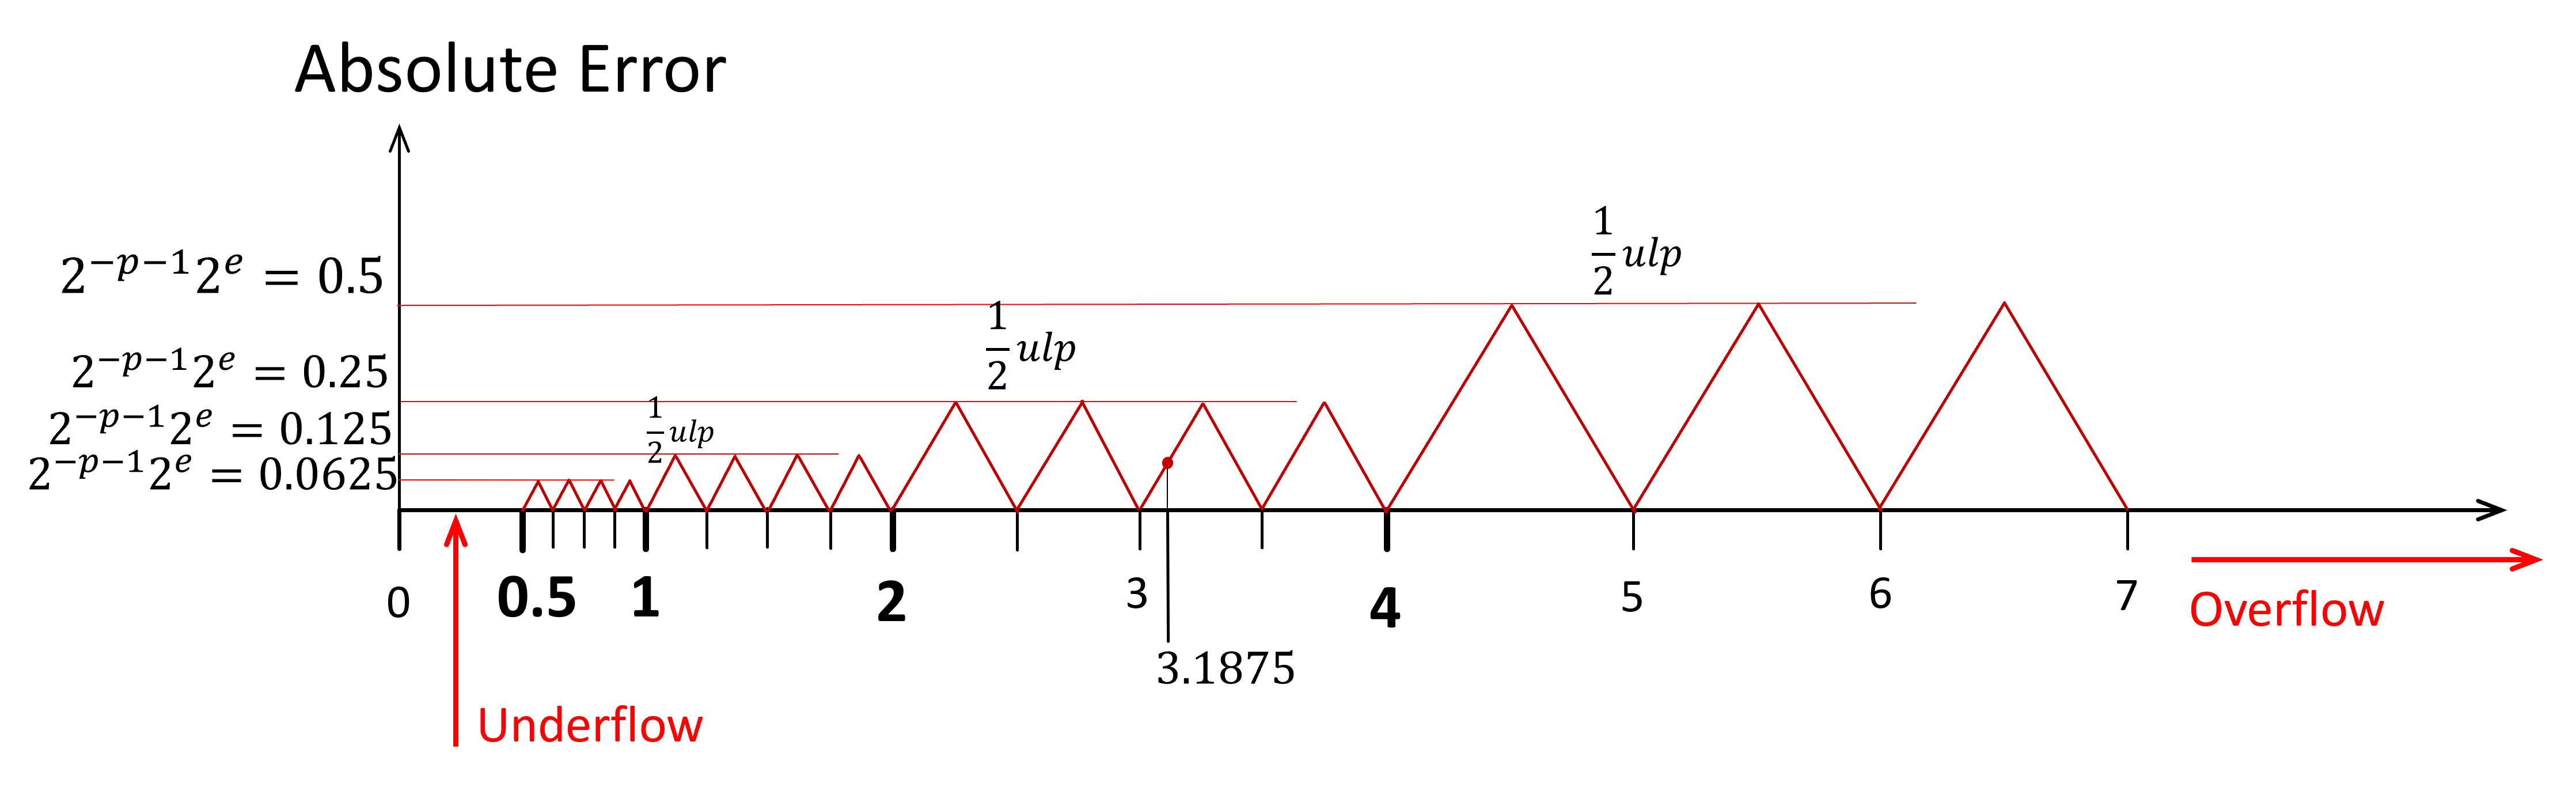
\includegraphics[width= \textwidth]{./doc/Figures/AbsErrorGraph.png}
%    \caption{Graphic of the absolute error committed when the real numbers are approximated by the nearest floating-point value with the 
%        maximum value represented for each window (exponent).}
%    \label{fig:AbsErrorGraph}
%\end{figure}
%
%\begin{figure}[h]
%    \centering
%    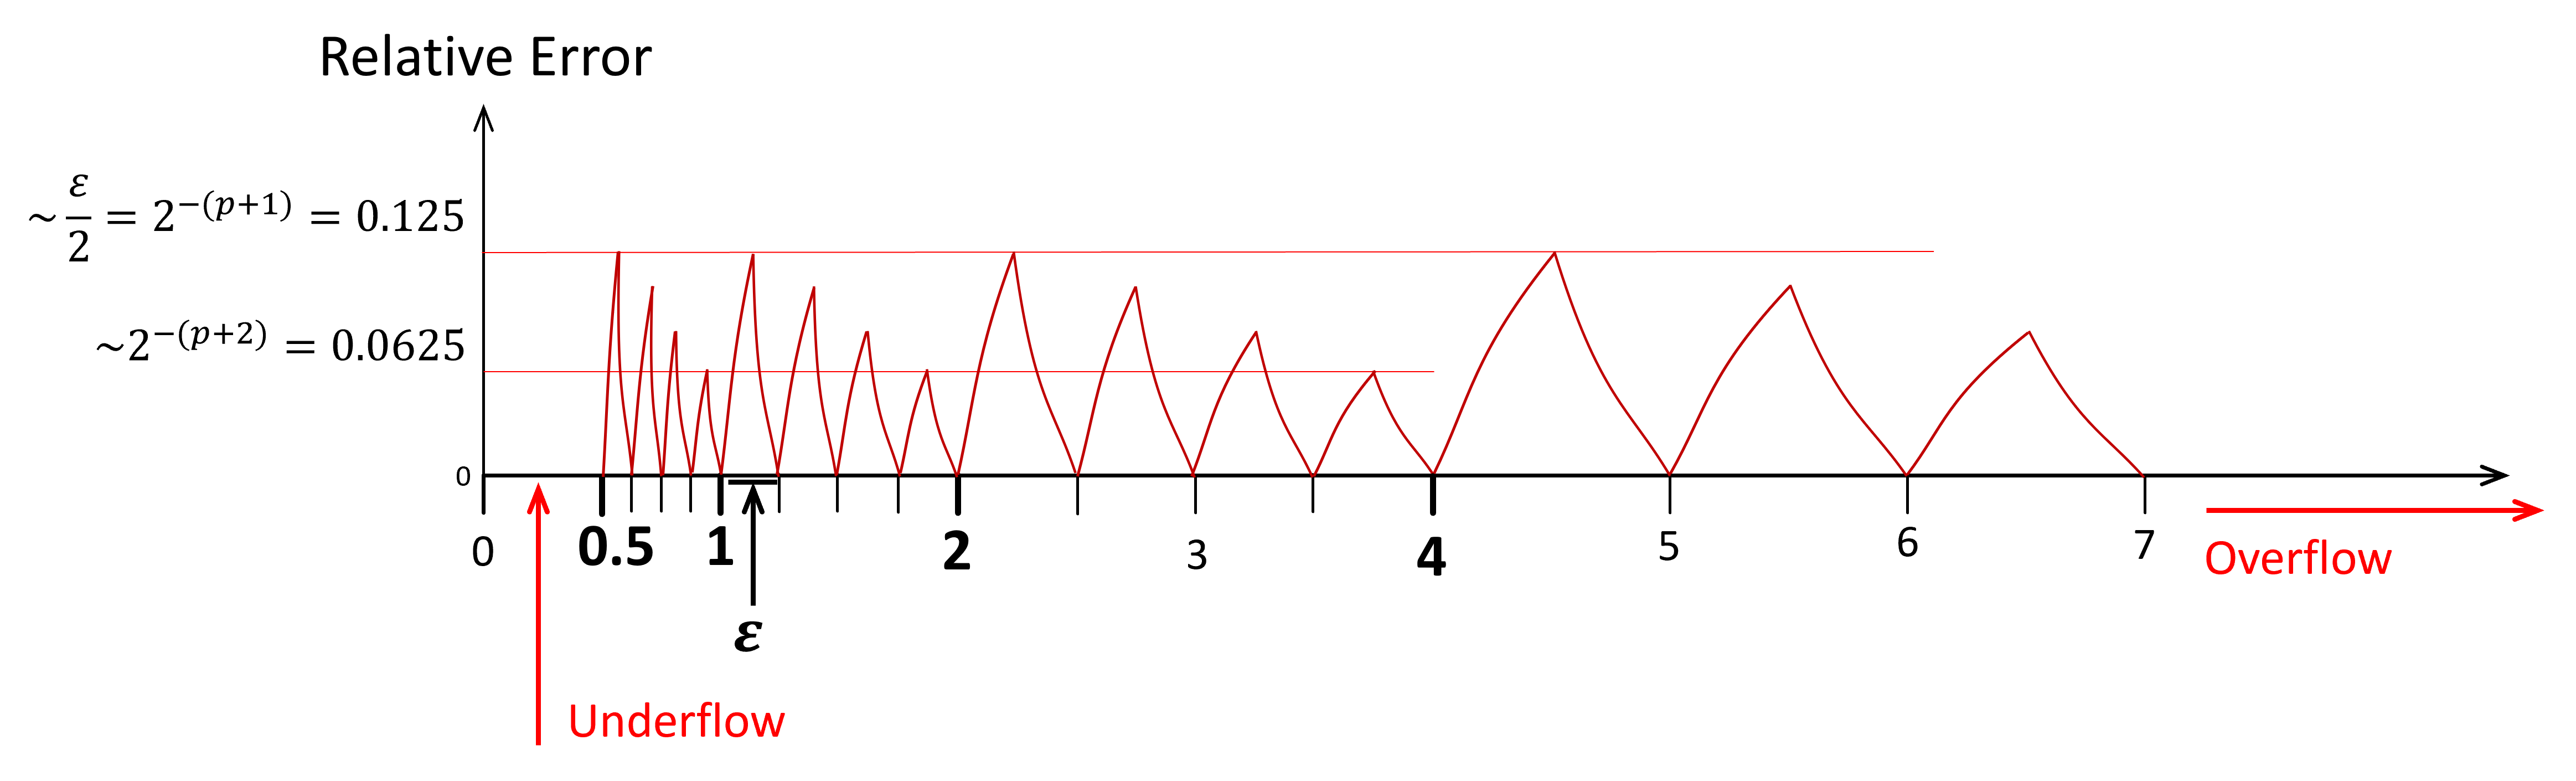
\includegraphics[width= \textwidth]{./doc/Figures/RelErrorGraph.png}
%    \caption{Graphic of the relative error committed when the real numbers are approximated by the nearest floating-point value with the 
%        maximum value represented for all windows (exponent).}
%    \label{fig:RelErrorGraph}
%\end{figure}
%
%\begin{IN}
%    The value $\frac{\beta}{2}\beta^{-p} = \epsilon$ is called machine epsilon, always take into account this magnitude because it bounds the 
%    relative error of any number when is rounded to the closest floating-point value. In the case of binary floating-point it can be 
%    expressed as $\epsilon = 2^{-p}$ taking the value of $2^{-24} \sim 5.96e-8$ in simple precision (23 bits plus 1 implicit bit), $2^{-53} 
%    \sim 1.11e-16$ in double precision and $2^{-113} \sim 9.63e-35$ in quadruple precision. In other conventions, the machine epsilon is 
%    considered the value $\beta^{1-p} = \epsilon$ which is the ulp for the value $1.0$ and in this case it is defined as: \textit{machine 
%        epsilon is defined as the difference between 1 and the next larger floating point number}.
%\end{IN}




    %--------------------------------------------------------------------------------------------------------------------------------------    
    \section{Decimal real number from its internal IEEE binary representation}


\FloatBarrier 
\begin{figure}[H]
    \centering
    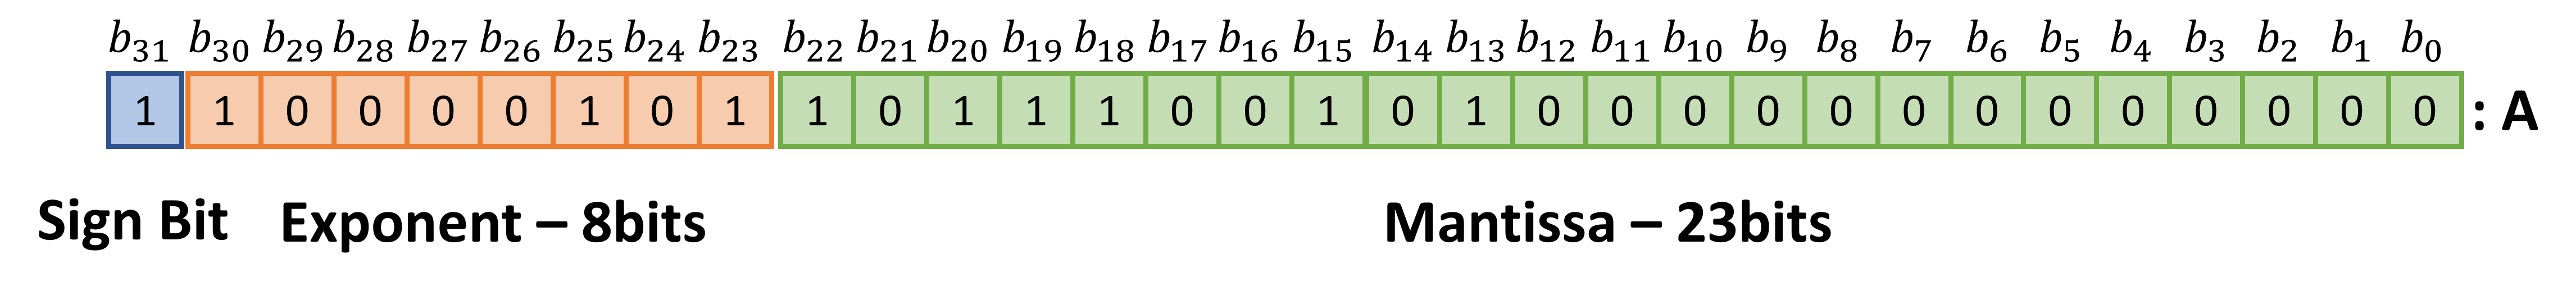
\includegraphics[width= \textwidth]{./doc/Figures/singlebits.png}
    \caption{Bit index for a single precision IEEE 754 floating-point (4 bytes).}
    \label{fig:singlebits}
\end{figure}

The decimal value for a single precision (\texttt{binary32}) floating point can be obtained trough the following expression (see Figure \ref{fig:singlebits}):
$$
   x = (-1)^{b_{31}}  \:  2^e  \: \left( 1 +   \sum_{i=1}^{23} b_{23-i} 2^{-i}    \right) 
$$
being $e$ the exponent already converted to decimal and properly biased. 
Notice that the implicit 1 is added to the sum which covers all the mantissa digits. 

The exponent uses a bias, also called  offset binary, to encode negative values $B = 2^{r-1} - 1 = 127$ ($r$ is the number of exponent digits). 
The following expression gives its decimal value:
$$
e = \sum_{j=0}^{7} b_{23+j} 2^j - B
$$
 

%The decimal value for a IEEE 754 floating-point value can be obtained trough the following expression (see Table \ref{tab:properties}):
%$$
%x = (-1)^{s}  2^e  \sum_{i=0}^{p} b_i 2^{-i} \quad \textnormal{with}\quad b_0 = 1
%$$
%being $s$ the sign bit, $e$ the exponent already converted to decimal and properly biased and $p$ the number of digits in the mantissa excluding the implicit 1. 
%Notice that $b_0 = 1$ considers the implicit 1 by adding $1\times2^0 = 1$ to the fractional mantissa.
% 
% The exponent uses a bias (or offset binary) to encode negative values. The following expression gives its decimal value:
% $$
% e = \sum_{j=0}^{r-1} b_j 2^j - \left( 2^{r-1} - 1 \right)
% $$
% being $r$ the number of exponent digits. 
 
\begin{IN}
    These expressions can be easily generalized by changing the bit index origins and upper limit of the sums:
    $$
    x = (-1)^{b_{p+r}}  2^e \left( 1 +   \sum_{i=1}^{p} b_{p-i} 2^{-i}    \right) 
    $$
    $$
    e = \sum_{j=0}^{r-1} b_{p+j} 2^j - B
    $$
    being $p$ the the number of digits in the mantissa (excluding the implicit 1), $r$ the number of exponent digits and $B = 2^{r-1} - 1$ (see Table \ref{tab:properties}).   
\end{IN}




 
 

%EJEMPLO
Now we can easily reconstruct the example in the Figure \ref{fig:ParametersIEEE}. Separating sign, exponent and mantissa we have the single precision binary: 

\texttt{1 10000101 10111001010000000000000}. 

The exponent is encoding the value:
$$
e = ( 2^0 + 2^1 + 2^7 ) - 127 = 6
$$
and the decimal value is:
$$
x = (-1)^1 \times 2^6 \times ( 1 + 2^{-1} + 2^{-3} + 2^{-4} + 2^{-5} + 2^{-8} + 2^{-10} ) = -110.3125_{10}
$$




%$$
%   \epsilon = m_1 2^e - m_2 2^e  = 2^{e-M} 
%$$
%Use scientific notation with ES format (normalized mantissa). 

    %--------------------------------------------------------------------------------------------------------------------------------------     
    \section{IEEE binary representation from decimal real numbers}

Let's revise the steps to encode a decimal number in IEEE 754 binary representation:

\begin{enumerate}
    \item Give a value to the sign bit: 1 for negative and 0 for positive.
    
    \item Convert the absolute value of your number to binary or similarly, to fixed-point representation. Right now there is not limit in the number of bits. 
      
    \item Move the binary point to the first position according to the binary scientific notation and then find the unbiased exponent.
    
    \item Omit the first 1, which will be implicit.
    
    \item Calculate the biased exponent by adding the bias $B = 2^{r-1}-1$ (check Table \ref{tab:properties}).
    
    \item Fill in the mantissa digits adding zeros at the right if necessary or truncating/rounding the excess of digits obtained in the conversion\footnote{The normal way to round the excess is by ``round to the nearest, ties to even''. If the (p+1)-th bit is a zero we chop the digits, if it is a 1 we add one to the p-th bit. The special case of a 1 in the (p+1)-th bit followed by zeros involves (similarly to the decimal system) that, if the p-th is a 1, we add one to the mantissa, if the p-th is a zero, we chop the digits.}.
\end{enumerate}




%EJEMPLO
Let's convert the number $-110.3125_{10}$ to a 32bits IEEE 754 floating point explaining step by step:

\begin{enumerate}
    \item This number is negative so the sign bit is a 1.
    
    \item The whole part is $110_{10}=\texttt{1101110}_2$ and the decimal part is $0.3125_{10}=\texttt{0.0101}_2$. Hence, the complete number in binary is:
    
     $\texttt{1101110.0101}_2$. 
    
    \item Moving the floating point: $\texttt{1101110.0101}=\texttt{1.1011100101} \times 2^6$.
    
    \item Omitting the implicit 1 we obtain the mantissa: 
    
    $\texttt{1.1011100101}\times2^6 \rightarrow \texttt{.1011100101}\times2^6$.
    
    \item To obtain the biased exponent we add $127$ since we are converting to single precision. Our exponent $6$ is covered by the value:
    
     $6 + 127 = 133_{10}= \texttt{10000101}_2$. 
    
    \item Writing the expressions for sign, exponent and mantissa and filling in the rest of mantissa digits with zeros at the right the result is: 
    
    $\texttt{1}\quad \texttt{10000101}\quad \texttt{10111001010000000000000}$
    
\end{enumerate}






    %-------------------------------------------------------------------------------------------------------------------------------------- 
    \FloatBarrier    
    \section{IEEE exceptions} \label{sec:exceptions}

The standard IEEE 754 reserves some combinations of binary digits for special situations: \texttt{NaN}, $\pm\infty$ or denormalised numbers (numbers in the gap that exits between the smallest normalised number representable (\texttt{tiny}) and the same negative value). In addition, take into account that there are two numbers equal to $0$: $\pm 0$ (see Table \ref{tab:SpecialValues}).

Infinity and NaN are essential to denote whether the result of a computation is too large to be represented in IEEE-754 (\textbf{overflow}) or a variable resulted in an illegal value (division $\frac{0}{0}$ for example). The operations between those special values are defined in the standard (see Table \ref{tab:SpecialOperations}).

The denormalised numbers (or subnormal numbers) are used when \textbf{underflow} occurs. Then, a gradual underflow is achieved so numbers too small to be represented (otherwise replaced by 0) are gradually decreased. From the representation point of view, the number is not treated with an implicit 1 before the binary point in the mantissa, but with a zero. Hence, the range of the mantissa is $\left[ 0, 1\right)$.


\begin{table}
    \centering
    \begin{tabular}{| c | c | l |}
        \hline
        Exponent & Mantissa & Value represented \\ \hline
        All 0's  & All 0's & $\pm 0 $ depending on the sign bit, they are equal  \\ \hline
        All 1's  & All 0's & $\pm \infty$ depending on the sign bit \\ \hline
        All 1's & NOT all 0's & Not a Number (\texttt{NaN})  \\ \hline
        All 0's  & NOT all 0's & Denormalised numbers  \\ \hline
    \end{tabular}
    \caption{Special binary combinations covered by the IEEE 754 standard.}
    \label{tab:SpecialValues}
\end{table}

\begin{table}
    \centering
    \begin{tabular}{| l | c |}
        \hline
        Operation & Result \\ \hline
        $ n / \left(\pm \infty\right) $            &     $	0$              \\ \hline
        $\pm \infty * \left( \pm \infty\right) $    &     $	\pm \infty$      \\ \hline
        $\pm$ nonZero$ / \pm 0 $            &    $	\pm \infty$       \\ \hline
        $\pm $finite$\quad * \pm \infty $      &    $	\pm \infty$       \\ \hline
        $\infty+\infty$  or  $\infty- \left(-\infty\right) $	     &       $+\infty$\\ \hline    
        $-\infty - \infty$   or  $-\infty + \left( -\infty \right) $   &        $	-\infty$\\ \hline
        $\pm 0 / \pm 0 $                  &        $	NaN$         \\ \hline
        $\pm \infty / \pm \infty $    &        $	NaN$     \\ \hline
        $\pm \infty * 0 $            &        $	NaN$     \\ \hline
        $ NaN == NaN $               &    $	False $      \\ \hline
    \end{tabular}
    \caption{Special operations covered by the IEEE 754 standard.}
    \label{tab:SpecialOperations}
\end{table}





    %--------------------------------------------------------------------------------------------------------------------------------------     
    \section{Declaring kind} 
    %\section{Practical guidance to use real numbers} 


Similarly to integers, a good practice is to write codes that can be used with different real precisions:
\texttt{kind=2, 4, 8}. To do that, do not specify the kind of any \textbf{variable}, just use \texttt{real :: x}. 
Then, the compiler assumes default real kind for all real variables. 
Generally, this default can be easily changed with a proper compilation option and then, 
the program does not depend on the precision imposed when it was written. 

The alternative is to explicitly declare the kind (precision) of any real variable: 
\begin{verbatim}
real(kind = 4) :: x1
real(kind = 8) :: x2
real(kind = 16) :: x3
\end{verbatim}

Instead of that, we propose to manage the compiler options and write with this notation:
\begin{verbatim}
    real :: x
\end{verbatim}

When declaring real \textbf{constants}, the situation is different. 
Consider for example the real constant \texttt{10.}. 
A specific kind type can be declared 
by underscoring the constant with its kind type or
by using exponential notation with \texttt{d} (double) or \texttt{q} (quadruple):

\newpage
\begin{verbatim}
10._4        
10._8    1d1     1.d1    1e1_8   1.e1_8
10._16   1q1     1.q1    1e1_16  1.e1_16
\end{verbatim}
However, this is not our recommended way to do it.

Consider not declaring the kind for any constant so it automatically adopts the default real kind value, use any of the following:
\begin{verbatim}
10.      1e1     1.e1    10e0   10E0    10.E0   10.e0
\end{verbatim}
First of all, notice that \texttt{10} can not be used since it would be treated as an integer. 
Secondly, remember that using exponential notation (\texttt{e} or \texttt{E}) does not automatically involves single precision. 
The \texttt{default real kind} compiler option rules its precision.

\begin{IN}
A program can be independent of declared precisions so the following compiler option rules the behaviour of all reals:

Default Real KIND: $\texttt{/real-size:{32\mid64\mid128}}$
\end{IN}






%RESTOS
%\begin{IN}
%    A program can be independent of declared precisions so the following compiler option rules the behaviour of all reals:
%    
%    Default Real KIND: $\texttt{/real-size:{32\mid64\mid128}}$
%    
%    Default Double Precision KIND: $\texttt{/double-size:{32\mid64\mid128}}$
%\end{IN}

%If the type of a variable is defined in the declaration of the variable it is typically used \texttt{real(kind = n) :: } or \texttt{real*n :: } where \texttt{n} is 4, 8 or 16. 
%Unless you have changed it, the default real kind is simple precision (\texttt{kind = 4}). 

%When declaring \textbf{constants}, the situation is different. 
%A specific kind type can be declared by underscoring the constant with its kind type:
%\begin{verbatim}
%    123.45_4
%    123.45_8
%    123.45_16
%\end{verbatim}
%However, this is not the common way to do it, 
%consider not declaring the kind for any constant neither so it automatically adopts the default real kind value.
%
%\textbf{Scientific notation} can also be used in languages like Fortran, for example, declaring the real constant $10.$ can be done equivalently in the following ways:
%\begin{verbatim}
%    10.
%    1e1
%    1.e1
%    10e0
%    10.E0
%    10.e0
%\end{verbatim}
%First of all, notice that \texttt{10} can not be used since it would be treated as an integer. 
%Secondly, remember that the kind of these constants \textbf{is not necessarily single precision}, default precision is being used with scientific notation so the \texttt{default real kind} option of the compiler rules the precision of these constants.
%
%Historically, if the scientific notation is mixed with the declaration of an specific kind, these declarations were used for double precision:
%\begin{verbatim}
%    1d1
%    1.d1
%    1e1_8
%    1.e1_8
%\end{verbatim}
%or for quadruple precision:
%\begin{verbatim}
%    1q1
%    1.q1
%    1e1_16
%    1.e1_16
%\end{verbatim}
%However, this is not our recommended way to do it, consider not declaring the kind for any constants so it automatically adopts the default real kind value.



    %--------------------------------------------------------------------------------------------------------------------------------------  
\newpage   
\section{\texttt{subroutine mantissa\_exponent\_base\_2}} 
The following subroutine allows to reconstruct a real number through its internal bits representation: 
%\vspace{0.5cm}
\listings{\home/IEEE_representation.f90}
{subroutine mantissa_exponent_base_2}{end subroutine}
{Subroutine to reconstruct the number in IEEE_representation.f90} 
This subroutine works by storing in a quadruple precision number any input value, 
either single, double or quadruple precision real. Then,  
the binary representation is written in a string called \texttt{bits}, 
the different parts are extracted (sign bit, exponent and mantissa) 
and the decimal value reconstructed. 
Notice the following: 
first, this code covers the normalized numbers and not the special values and denormalized numbers. 
Second, the conversion to quadruple precision carries with the round off error of the original precision and 
third, in order to write bits in the screen do not forget that leading zeros are not displayed.

Functions \texttt{normalized\_mantissa(string)} and \texttt{biased\_exponent(string)} returns the mantissa including an implicit 1 and the exponent biased with a bias value of 16383 from the input string of bits. 

\listings{\home/IEEE_representation.f90}
{function normalized_mantissa}{end function}
{normalized_mantissa function in IEEE_representation.f90} 

\listings{\home/IEEE_representation.f90}
{biased_exponent}{end function}
{biased_exponent function in IEEE_representation.f90} 

Call the program with the same real value declared as simple, double and quadruple precision and take a care look at the big differences in the reconstructed number, specially the significant digits for all the precisions. 







 






































%------------------------------------------------------------------------------------------------------------------------------------------------------
%------------------------------------------------------------------------------------------------------------------------------------------------------
%------------------------------------------------------------------------------------------------------------------------------------------------------
%------------------------------------------------------------------------------------------------------------------------------------------------------
%A FUTURO


%Poner ejemplos del epsilon en fortran
%Ver lo codigos que ya tengo hechos. Detalle de como mostrar resultados
%Recomendacion en la notacion


%Acabar el articulo de What Every... y capítulo de Trefethen


%
%This information can also be accessed by code, take a look at the useful intrinsic functions that can be used in Fortran.
%
%\begin{verbatim}
%    real(kind=4) :: x
%    real(kind=8) :: y
%    
%    write(*,*) 'Declaration of x with - real(kind = 4):: x'
%    write(*,*) 'Maximum value', huge(x)
%    write(*,*) 'Minimum value', tiny(x)
%    write(*,*) 'Round_off', epsilon(x)
%    write(*,*) 'Significant digits', precision(x)
%    
%    write(*,*) 'Declaration of y with - real(kind = 8) :: y'
%    write(*,*) 'Maximum value', huge(y)
%    write(*,*) 'Minimum value', tiny(y)
%    write(*,*) 'Round_off', epsilon(y)
%    write(*,*) 'Significant digits', precision(y)
%\end{verbatim}
%
%which results in:
%
%\begin{verbatim}
%    Declaration of x with - real(kind = 4):: x
%    Maximum value  3.4028235E+38
%    Minimum value  1.1754944E-38
%    Round_off  1.1920929E-07
%    Significant digits           6
%    
%    Declaration of y with - real(kind = 8) :: y
%    Maximum value  1.797693134862316E+308
%    Minimum value  2.225073858507201E-308
%    Round_off  2.220446049250313E-016
%    Significant digits          15
%\end{verbatim}



    %--------------------------------------------------------------------------------------------------------------------------------------
% \section{Operations}

%Take a look at the following example of simple arithmetic operations between different data types (whether different type or kind in the same type):
%
%\begin{verbatim} 
%    write(*,'(a20, f17.15)') '1.1/2.        ', 1.1/2. 
%    write(*,'(a20, f17.15)') '1.1e0/2e0     ', 1.1e0/2e0
%    write(*,'(a20, f17.15)') '1.1d0/2d0     ', 1.1d0/2d0 
%    
%    write(*,'(a20, f17.15)') '1.1/2         ', 1.1/2
%    
%    write(*,'(a20, f17.15)') '1.1/2d0       ', 1.1/2d0
%\end{verbatim}
%
%The result when the compiler has default real kind defined as simple precision is the following, try to understand why those results:
%
%\begin{verbatim}
%    1.1/2.        0.550000011920929 
%    1.1e0/2e0     0.550000011920929 
%    1.1d0/2d0     0.550000000000000 
%    
%    1.1/2         0.550000011920929 
%    
%    1.1/2d0       0.550000011920929 
%\end{verbatim}
%
%Let's analyse each example and obtain some conclusions from them. 
%
%The first three examples performs the same operation, it divides the number \texttt{1.1} (which does not have exact representation in the standard IEEE 754) by two, which is exact. They perform the operation with no precision imposed the first two of them and in double precision the third one. However, if we change the default real kind in the compiler options and impose to treat constants and variables as double precision by default, the result is:
%
%\begin{verbatim}
%    1.1/2.        0.550000000000000
%    1.1e0/2e0     0.550000000000000
%    1.1d0/2d0     0.550000000000000
%\end{verbatim}
%
%The conclusion to obtain from this is: write codes that do not depend on a precision, just use the first case (\texttt{1.1/2.}) and change the compiler options whether you need simple precision or double precision result. It is not necessary to write in each operation \texttt{d0} to make sure that the operation is performed in double precision, just configure the compiler to treat all constants (and variables) as double precision. In the next example it is demonstrated that writing (\textit{2.}) is not necessary neither. However, notice that in order to force the constant to be real (\texttt{e0}) is not needed. 
%
%Now take a look at the fourth example, it uses the integer 2 instead of converting it to a real number. While operations between two integer operands or between two real operands are developed as expected, a mixed-mode expression (where different data types are involved) must be treated with care. Arithmetic involving different types of operands or different kinds of the same type (i.e. \texttt{real (kind 4)} and \texttt{real (kind 8)}) will be carried out by converting the lowest-ranking operand to the highest-ranking operand so the result has this type and kind. The table \ref{tab:ranking} shows the ranking of each type. 
%
%\begin{table}[h]
%    \begin{tabular}{| c | c |}
%        
%        \hline
%        Data Type & Ranking \\ \hline
%        LOGICAL(1) and BYTE & Lowest \\ \hline
%        LOGICAL(2)     &  . \\ \hline
%        LOGICAL(4)     &  . \\ \hline
%        LOGICAL(8)      & . \\ \hline
%        INTEGER(1)     &  . \\ \hline
%        INTEGER(2)    &   . \\ \hline
%        INTEGER(4)    &   . \\ \hline
%        INTEGER(8)    &   . \\ \hline
%        REAL(4)     &  . \\ \hline
%        REAL(8)     &    .   \\ \hline
%        REAL(16)    &   . \\ \hline
%        COMPLEX(4)  &     . \\ \hline
%        COMPLEX(8)  &     . \\ \hline
%        COMPLEX(16) &    Highest\\ \hline
%        
%        
%    \end{tabular}                                                       
%    \caption{Ranking assigned to each data type, arithmetic will be performed with the highest ranking.}
%    \label{tab:ranking}
%\end{table}
%
%This means that the integer 2 is automatically converted to a real value (which has higher-ranking associated) and the operation is performed. If double precision is needed is simple, just change the compiler option and execute the same program:
%
%\begin{verbatim}
%    1.1/2         0.550000000000000
%\end{verbatim}
%
%The main conclusion is that there is no need of specifying always that constants are real values if the operation is performed with one operand being already real. But do not forget that at least one operand must define the type of operation to perform, if you do not write at least one real value, you are operating in the integers field and the divisions in the integer field totally ignore the decimal part of the result, so it is truncated (the rest of the operations in the integer field are performed as expected):
%
%\begin{verbatim}
%    write(*,'(a20, f17.15)') '1/3           ', 1/3
%\end{verbatim}
%
%which results in the :
%
%\begin{verbatim}
%    1/3           0.000000000000000
%\end{verbatim}
%
%The situation can be tricky when more operands are involved: 
%
%\begin{verbatim}
%    write(*,'(a20, f17.15)') '5/2 * 3. =      ', 5/2 * 3.
%    write(*,'(a20, f17.15)') '3. * 5/2 =      ', 3. * 5/2
%\end{verbatim}
%
%\begin{verbatim}
%    5/2 * 3. =      6.000000000000000
%    3. * 5/2 =      7.500000000000000
%\end{verbatim}
%
%Both are the same operation, however the first example is not properly performed since the precedence of the operation is from left to right in products and divisions. Hence, 5/2 is operated in first place, and the result is 2 in the integer field, which multiplied by 3. is 6. At least, in the division, it would be nice to force one value to be real with no need of changing the order of the operation. 
%
%Take a look at the following examples in real situations:
%PONER EJEMPLOS REALES
%%Ejemplo de dividir por 2. en grids
%%Otros ejemplos
%%Poner el caso de variable constante N que hay que pasar a real usando real(N) FUNDAMENTAL
%
%
%Finally, look at the fifth example, it can be a little tricky to understand at first. Notice that the compiler is configured for default real kind in simple precision so the value 1.1 is simple precision. According to the table above we could think that the value 1.1 is transformed to double precision in order to be operated with the value \texttt{2d0}. However, the result is clearly carrying with the round-off of the value 1.1 in simple precision. The reason is that the value 1.1 is stored in double precision but no transformed to double precision. 
%
%%Aqui poner los bits de este ejemplo
%
%If the same code is executed with default double precision then the value 1.1 is already double precision so there is not problem. Once again, according to our first conclusion, writing \texttt{2d0} in both cases is not necessary at all and just blurs the program.
%
%\begin{verbatim}
%    1.1/2d0       0.550000000000000
%\end{verbatim}
%
%%Profundizar en UNA sola operacion entre dos numeros, que precision asegura. epsilon y epsilon de la maquina
%
%
%
%
%To be explained:
%
%\begin{verbatim} 
%    x**2  = x * x 
%    
%    y = 2 * x 
%    
%    y = 2d0 * x 
%    
%    y = 2. * x 
%    
%    x**2d0 = exp( 2 * ln x ) 
%    
%    
%    x = 1 / 2
%    x = 1 / real(2) 
%    x = 1 / 2. 
%    
%    x = 1d0 * i / N  ! NO GUSTA 
%    
%    x = i / real(N) 
%    
%    ! same numbers 
%    x = 1 
%    x = 1. 
%    x = 1D0 
%    x = 1e0 
%    
%    y = x**2
%    y = x**2.
%    
%\end{verbatim} 






%------------------------------------------------------------------------------------------------------------------------------------------------------
%------------------------------------------------------------------------------------------------------------------------------------------------------
%------------------------------------------------------------------------------------------------------------------------------------------------------
%------------------------------------------------------------------------------------------------------------------------------------------------------
%RESTOS


%\newpage
%\begin{table}[H]
%    \begin{flushright}
%        \begin{turn}{90}
%            \begin{tabular}{| r | c | c | c | c | c | c | c | c |}
%                
%                \hline
%                Name & Sign & Exp. & Mantissa & Exp. Bias & Bits precision & \begin{tabular}{@{}c@{}}Normalized \\ range \end{tabular}   & Approximate decimal  & Precision \\ \hline
%                
%                \begin{tabular}{@{}c@{}}Single precision \\ (binary32) \end{tabular}      & 1 & 8  & 23    & +127   & 24 & \begin{tabular}{@{}c@{}}$\pm2^{−126}$ to \\$\pm2^{127+1}$  \end{tabular}    & \begin{tabular}{@{}c@{}}$\pm1.18\cdot10^{ −38}$ to \\ $\pm3.4\cdot10^{38}$ \end{tabular}     & \sim 7.2 digits  \\ \hline
%                
%                \begin{tabular}{@{}c@{}}Double precision \\ (binary64) \end{tabular}    & 1 & 11 & 52    & +1023  & 53 & \begin{tabular}{@{}c@{}}  $\pm2^{−1022}$ to\\  $\pm2^{1023+1}$\end{tabular}  & \begin{tabular}{@{}c@{}} $\pm2.23\cdot10^{ −308}$ to \\ $\pm1.80\cdot10^{308}$ \end{tabular} & \sim 15.9 digits        \\  \hline
%                
%                \begin{tabular}{@{}c@{}} Quadruple precision\\(binary128) \end{tabular}   & 1 & 15 & 112   & +16383 & 113 & \begin{tabular}{@{}c@{}}  $\pm2^{-16382}$ to\\  $\pm2^{16383+1}$\end{tabular}   & \begin{tabular}{@{}c@{}} $\pm3.3621\cdot 10^{-4932}$ to \\ $\pm1.1897\cdot10^{4932}$ \end{tabular}  & \sim 19.2 digits          \\ \hline
%                
%            \end{tabular}                                                       
%        \end{turn}
%        \caption{Main properties of the different precisions covered by the IEEE 754 standard.}
%        \label{tab:properties}
%    \end{flushright}
%\end{table}

%\newpage
%\begin{table}[H]
%    \begin{flushleft}
%        \begin{turn}{90}
%            \begin{tabular}{| r | c | c | c | c | c |}
%                
%                \hline
%                Name & Sign bits & Exp.bits & Mantissa bits & Exp. Bias & Bits precision \\ \hline
%                
%                \begin{tabular}{@{}c@{}}Single precision \\ (binary32) \end{tabular}      & 1 & 8  & 23    & +127   & 24  \\ \hline
%                
%                \begin{tabular}{@{}c@{}}Double precision \\ (binary64) \end{tabular}    & 1 & 11 & 52    & +1023  &   53  \\  \hline
%                
%                \begin{tabular}{@{}c@{}} Quadruple precision\\(binary128) \end{tabular}   & 1 & 15 & 112   & +16383 & 113 \\ \hline
%                
%            \end{tabular}                                                       
%        \end{turn}
%        \caption{Fruta disponible}
%        \label{tab:properties}
%    \end{flushleft}
%\end{table}
%\begin{table}[H]
%    \begin{flushright}
%        \begin{turn}{90}
%            \begin{tabular}{| r | c | c | c |}
%                
%                \hline
%                Name & \begin{tabular}{@{}c@{}}Normalized \\ range \end{tabular}   & Approximate decimal  & Precision \\ \hline
%                
%                \begin{tabular}{@{}c@{}}Single precision \\ (binary32) \end{tabular}      &  \begin{tabular}{@{}c@{}}$\pm2^{−126}$ to \\$\pm2^{127+1}$  \end{tabular}    & \begin{tabular}{@{}c@{}}$\pm1.18\cdot10^{ −38}$ to \\ $\pm3.4\cdot10^{38}$ \end{tabular}     & \sim 7.2 digits  \\ \hline
%                
%                \begin{tabular}{@{}c@{}}Double precision \\ (binary64) \end{tabular}    &  \begin{tabular}{@{}c@{}}  $\pm2^{−1022}$ to\\  $\pm2^{1023+1}$\end{tabular}  & \begin{tabular}{@{}c@{}} $\pm2.23\cdot10^{ −308}$ to \\ $\pm1.80\cdot10^{308}$ \end{tabular} & \sim 15.9 digits        \\  \hline
%                
%                \begin{tabular}{@{}c@{}} Quadruple precision\\(binary128) \end{tabular}   & \begin{tabular}{@{}c@{}}  $\pm2^{-16382}$ to\\  $\pm2^{16383+1}$\end{tabular}   & \begin{tabular}{@{}c@{}} $\pm3.3621\cdot 10^{-4932}$ to \\ $\pm1.1897\cdot10^{4932}$ \end{tabular}  & \sim 19.2 digits          \\ \hline
%                
%            \end{tabular}                                                       
%        \end{turn}
%        \caption{Fruta disponible}
%        \label{tab:properties}
%    \end{flushright}
%\end{table}




       %

\section{Condition number and stability} 
    
The condiotn number of a problem do not know anything about the operations 
and the round-off errors associated to the algorithm.  

An algorithm is stable is every step is well conditioned. 

Round-off + unstable = disaster. (e.g. alternate series)

Round-off + stable = bounded error. 

Exact arithmetic (no round-off errors) stability is not concerned. 
Well/Ill condiotned refers to the problem 

stability refers to the algorithm. 

Example. condition number at x = 0 is one but it is unstable. 

 
$$
y = \sqrt{1+x} - 1 
$$   


Examples: 
\begin{enumerate} 
\item $1+ x $ no problme
\item $ \sqrt{1+x} $ no problem 
\item substract  $ \sqrt{1+x} - 1 $ :BIG PROBLEM 

\end{enumerate}
look for another algorithm 
$$
y =  \frac{x}{\sqrt{1+x} + 1}
$$

Backward stability. The significance of the error produced by the algorithm is due only to
the conditioning of the problem. 


Multiplications no problem 

Substractions near equal values 
$$ 
k = \frac{ | x | }{ |x - y |}
$$   
    
    $$
     k = \frac{ f(x+\Delta x) - f(x) }{ f(x)} / \frac{ \Delta x  }{ x} = \frac{ f^\prime(x) x }{ f(x)}  
    $$
    
    $$
        \frac{\Delta y}{ y }  =  = \frac{ f^\prime(x) x }{ f(x)}  \frac{\Delta x}{ x}
    $$
    
    
    Stability 
    $$
      \frac{\tilde{f} (x) - f(x)   }{ f(x) }
    $$

Examples: 
\begin{enumerate} 
\item $\sqrt{x^2+1} -1$ 
\item $ \frac{1- cos(x)}{ x^2} $ = $ 0.5 ( \frac{ sin(x/2)}   {x/2 } )^2 $
\item plot $ y = (x-2)^9 x \in [ 1.95, 2.05] $ 1000 points 


\end{enumerate}




 \usetikzlibrary{shapes.geometric, arrows}
 
 \usetikzlibrary{positioning} 
 
 \tikzstyle{block} = [draw, rectangle, rounded corners, draw=black, very thick,
 fill={rgb:orange,1;yellow,2;pink,5},
 text width=4cm, text centered, minimum height=1.2cm, node distance=3cm]
 
 \tikzstyle{blockr} = [draw, rectangle, rounded corners, draw=black, very thick,
  fill={rgb:red,1;red,2;red,5},
  text width=4cm, text centered, minimum height=1.2cm, node distance=3cm]
 
 \tikzstyle{container} = [draw, rectangle, inner sep=0.3cm]
 
 \tikzstyle{text} = [draw, color=blue]
 \tikzstyle{arrow} = [thick,->, >=latex]
 \tikzstyle{line} = [thick,-]
 
 
 \begin{figure}[]
 	\centering
 	
 	\begin{tikzpicture}
 	
 
 	\node [block] (m) {Math model} ;
 	\node [block, below right=2cm and -1cm of m] (a) {Algorithm};
    \node [blockr, below left=2cm and -1cm of m] (n) {\textcolor{white}{New math model}};
 	\node [blockr, below left=2cm and -1cm of a] (na) {\textcolor{white}{Change the algorithm}};
 	\node [block, below right=2cm and -1cm of a] (p) {Implement};
 
 
 	\draw [arrow] (m) -- (a);
 	\draw [arrow] (m) -- (n);
 	\draw [arrow] (a) -- (p);
 	\draw [arrow] (a) -- (na);
 	
 
 
 
 	
 
 	\node [color=blue, below right=0.5cm and -1.5cm of m ]  {Well-conditioned};
 	\node [color=red, below left=0.5cm and -1.5cm of m ]  {Ill-conditioned};
 	\node [color=blue, below right=0.5cm and -1.5cm of a ]  {Stable};
 	\node [color=red, below left=0.5cm and -1.5cm of a ]  {Unstable};
 
 
 	
 	
 	\end{tikzpicture}
 	
 	\caption{Software Development Life Cycle }
 \end{figure}





  

\newpage    
\section{Common numerical errors}

    
    
\listings{\home/Round_off.f90}
{errors_in_operations}{end subroutine}
{Round_off.f90} 



\newpage    
\section{Catastrophic cancellation}  \label{sec:cancellation}
    
    
\listings{\home/Round_off.f90}
{catastrophic_cancellation}{end subroutine}
{Round_off.f90} 





\newpage    
\section{Truncation errors and round-off errors}
    
     
\listings{\home/Summation_errors.f90}
{summation_example}{end subroutine}
{Summation_errors.f90} 



\newpage    
\section{IEEE exception examples}
    
    
\listings{\home/IEEE_operations.f90}
{IEEE_exception_examples}{end subroutine}
{IEEE_operations.f90} 






\section{TO MERGE}


1. Calculando el epsilon correcto suma hasta un cierto error en modo debug
2. En ese caso Debug sumar 10000000 de terminos no supone diferencia porque son numeros que no se pueden sumar ya
3. Sumar hacia atras si reduce enormemente el errror de floating en cada suma y consigue mucha mas exactitud

4.Pero la suma hacia delante si se hace con el modo Release optimiza el bucle y calcula con  mas precision 10000000 de terminos de la suma que el caso en el que para en el epsilon que le corresponde. Esto es magia del compilador que optimiza y seguramente haga sumas parciales hacia atras y por eso da mas exactitud. 

5. Correr en modo release pero pedir que lo pinte dentro del bucle hace lo mismo que debug porque no es capaz de aplicar la optimizacion si le pides que pinte cosas entre medias. 

In the context of floating-point representation, the intrinsic function $\epsilon$ represents the smallest 
number that added to 1 results in a number higher than 1.
This value depends on the number of binary digits reserved to store the floating-point
value (as it is covered in the section \ref{chap:reals}). 

It seems clear that adding a number higher than $\epsilon/2$ to 1
will be captured by the floating-point precision jumping to the value $1 + \epsilon$, a lower value will not be added
since the result is closer to 1 (and further from $1 + \epsilon$). For a number different than 1, let's say for example $S = 12.54$ a slight 
modification of the epsilon is needed. However, the idea is the same, the floating-point value does not allow 
adding more terms to $ S $ when those values are less than $\epsilon/2$. 


%Notice that $S(1 + \epsilon) = S + S\epsilon$ represents an upper bound 
%for the nearest floating-point value to $S$. Hence, adding values smaller than $S\epsilon$ to the number $S$ 
%will not be captured in the result. 




%First, take a look at the result of the computer if the summation process is stopped according to the 
%floating-point error due to the significant digits. Notice that this result is obtained after 2260 sums
%and the truncation error has the main part.
%
%\begin{verbatim} 
%    Total Error = 4.4035912E-04
%    Truncation Error = 4.4247787E-04
%    Floating-point Error = -2.1187589E-06
%\end{verbatim}
%
%Now try to calculate the same sum up to 10000000 terms, notice that the total error is similar to the 
%previous case, a little lower at cost of 4 thousand times the number of sums performed, 
%but now the floating-point error has the main contribution for the total error. 
%
%\begin{verbatim} 
%    Total Error = 2.0885468E-04
%    Truncation Error = 1.0000000E-07
%    Floating-point Error = 2.0875467E-04
%\end{verbatim}
%
%In addition, there is another way of calculating this sum with better accuracy in the computer apart from 
%using higher precision for the variables. This is a non-intuitive way of calculating the sum that comes from the fact
%that adding in floating-point arithmetic is not an associative operation. 
%Let's perform the same sum backwards, with simple precision also and from the lower terms to the higher ones using 10000000 terms. 
%
%\begin{verbatim} 
%    Total Error = 2.3841858E-07
%    Truncation Error = 1.0000000E-07
%    Floating-point Error = 1.3841859E-07
%\end{verbatim}
%
%As a general rule, when adding terms with really different orders of magnitude try to sum first the lower values and then add the result to the higher values.



%An extensive discussion regarding the consistency of using \texttt{epsilon( S )} for this example and the generalization for any other sum 
%is treated in the section \ref{chap:reals} of Part \ref{PartII} of this book. Also, why dividing it by \texttt{2} is needed becomes clearer. Some notions of 
%floating-point representation are essential to deepen in these topics. 

       
   
   
  
  \part{Advanced programming}\label{PartIII}
       \chapter*{Menu for Advanced Programming} 
    
    \vspace{-1.5cm}
    \subsection*{Fortran menu}
    \vspace{0.5cm}
    \renewcommand{\home}{./Fortran/sources/Advanced_programming} 
    \lstfor
     \listings{\home/advanced_programming.f90}{Advanced programming}{Wrapper}
              {advanced_programming.f90}
   
    \subsection*{Python menu}
    \vspace{0.5cm}
      \renewcommand{\home}{./Python/sources/Advanced_programming} 
      \lstpython
       \listingsp{\home/advanced_programming.py}{while}{Wrappers}
                {advanced_programming.py}
                
 
 
 
 
 
 
 
  
\chapter{Overview} 
One of the main characteristics to reuse code is generic programming.  
Generic programming is based on abstract variable types that are then instantiated 
when they are used for specific variable type.

Since Python is non typed language, 
generic programming in this language is straightforward. 
However, in Fortran the use of abstract  \lstinline{class(*)} 
allows to use different data types at run time. 
  
 
    \newpage            
    \section{Scope} 

One of the most important matters that we need to understand when we begin to write our own codes in any programming language is the scope. 
The scope of variables, named constants, objects, functions or procedures is the area of the program where they can be used or modified, that is, the area where each object is visible.

The example that best illustrates this concept is a variable \texttt{c} declared inside a function \texttt{f( x )}. 
This variable named \texttt{c} can be initialized, used and modified inside the function. 
However, outside this area, \texttt{c} is not seen or the name \texttt{c} could refer to a totally different entity. 
In this case \texttt{c} is said to be a \textit{local variable}.
When a variable is declared at the beginning of a program, outside the scope of any function, it is said to be a \textit{global variable} and it can be used everywhere in your program unless you intentionally limit its scope. 

Notice that \textit{global} and \textit{local} sometimes refer to those entities that are seen by the whole program or just some parts of the code, respectively. 
On other occasions, \textit{global} and \textit{local} entities refer to one specific unit of program/subprogram, for instance, a variable declared at the beginning of a module is a \textit{global} variable for that module, so any subroutine or function defined inside will see it. However, this does not necessarily mean that the variable is seen by the main unit of program that uses this module. 

%Another example is the variable declared at the beginning of a subroutine that has a function declared inside, it is considered a global variable for the subroutine and functions nested but it is considered local according to the main program. 

Each programming language has its own set of rules to consider entities as global or local, however, sometimes the programmer can limit or enlarge the scope.
The statements \texttt{public} and \texttt{private} change the scope of entities in Fortran so they can be accessed or not outside a module.
Hence, private variables or procedures are specified explicitly. Otherwise, global module variables are visible outside by default.   

Scope is an essential concept when talking about modular programming and encapsulation. Some constants may be placed at the beginning of the code as global entities so every part of the code can see the same value (e.g. \texttt{pi = 4 * atan(1)}), in this case it is strongly recommend to use the \texttt{parameter} attribute so its value can not change during the execution. However, we want each subprogram unit to use their own set of variables and constants without interfering with the rest of parts of the program. Furthermore, we also want every subprogram to use only local variables so everything needed is either declared inside or passed via parameter. 
As a general rule, the use of global variables should be reduced as possible, these entities can be easily modified unintentionally leading to hard to fix bugs.  



    \section{Functional Programming}
Scientific programming is very close 
to mathematics. Numerical schemes and approximation are grounded on vector spaces of finite and 
infinite dimensions. Hence, experts developers have a deep knowledge of mathematics and they 
feel conformable when writing in codes that mimic the mathematical functions. 
Functional programming paradigm allows mathematician to talk the same language that they are used to. 
There are also other reasons why functional programming is growing in popularity. 
\begin{enumerate}
\item Complex simulations involve complex process of data. Functional programming avoids 
the control flow by concentrating in what to do. When complexity grows exponentially, 
functions should work independently of the outer world. 
\item Hierarchical knowledge based on function composition and abstraction layers. 
Functional programming is grounded on lambda calculus and in function composition concepts that 
allow to build huge codes with different abstraction layers organized in a knowledge hierarchical fashion. 
\item Parallel programming. 
Since computational requirements are growing with more realistic simulations, parallel programming is
becoming a common reality. Different functions are run simultaneously in different processors. 
 Functional programming adapts flawlessly to the parallel programming 
strategy by minimizing side effects with pure functions. 
\end{enumerate}
Object oriented languages tend to be imperative performing actions sequentially.  
Sentence are  put in order to understand how the program performs and variables are followed
to achieve the desired result. On the contrary, when developing codes with functional 
programming paradigm, the driver is the function or what to do. 
Functional programming is  declarative which means that functions are built by functional composition
and no flow control is followed. Its power lies in declarativity and expressivity.

Functional programming concentrates on operations like mapping which transform a complete set 
of elements in another set or collection of objects by means of a pure function.  
There is no need to follow the flow ot the program to check the right performance of the operation. 
It looks really elegant.

Everything started with the hardware.
Imperative style suited better for hardware due to the von Neumann architecture. 
John Backus in 1977 asked in his famous Turing Award lecture:
 "Can Programming Be Liberated from the von Neumann Style?". 
 It was the origin of functional programming. 


\newpage 
    \section{Overloading} 
Scientific programming has common operations that are performed for different 
space domains or different data types. In those cases, functions or operators can be  overloaded 
to generalize different types or data structures.  
Overloading is usually referred to:  
\begin{enumerate}
\item Function overloading.
\item Operator overloading.
\end{enumerate}
Functional overloading refers to creation of multiple functions with the same name but with different implementations. 
Calls to an overloaded function will run a 
specific implementation of that function depending on the arguments of the call. 
Function overloading is usually named: static polymorphism in which a function call is resolved by matching 
type, kind and rank of actual arguments with a function with same type, kind and rank of dummy arguments.
Function overloading is usually associated with statically-typed programming languages such as Fortran. 
The determination of which function to use for a particular call is resolved at compilation time.
Those languages which are untyped, such as Python, do not support function overloading. 


Operator overloading complements the definition of classical operators for operands of new types. 
For example, the operator \verb|*| is natively overloaded for real or complex numbers. 
In automatic differentiation technique, dual numbers 
$$ z = a + b \epsilon
$$ 
with $\epsilon^2=0$ 
are defined to calculate exact derivatives of real functions. 
If basic operators and intrinsic functions are overloaded for those dual numbers, 
this technique allows to calculate 
exact derivatives of real functions is implemented very easily. 

Operator overloading is syntactic sugar which means that things are made easier to read or to express.
It makes the language "sweeter" for human use.
Sometimes, operator overloading is termed operator {\it ad hoc} polymorphism.
In scientific computing, operator overloading allows to manipulate objects with the same syntax as on paper.



    \newpage 
    \section{Object Oriented Programming}

Contrary to functional programming, object-oriented programming is not born 
from strong mathematical foundations but from the need of describing the solution to a problem 
by creating simulations of real life systems.

This programming paradigm is based on the concept of \textit{object} which presents 
a state in the form of data (usually called properties) and 
a behaviour in the form of procedures (usually called methods).
In addition, an object has identity, an unique name that differentiates it from other objects. 
Hence, an object ties together what is it and how it relates.

There are similar ideas behind the category theory of mathematics.
But also, the definition of some objects in common branches of mathematics follow a pattern similar to the mentioned. 
Sometimes a mathematical object is defined by what they do together with what they are. 
Notice for example the definition of a field, it has a set which could be identified with 
its state, but also two operations that must accomplish with a bunch of axioms. 
This could be identified with its behaviour. 

%Ejemplo de un objeto
Let's see what classes and objects are through an example. 
Imagine you want to simulate the evaporation of a bunch of spherical fluid droplets. 
Each droplet presents an state like its temperature, its size, the mass fraction of fluid at its surface, a spatial discretization to solve conservation equations, etc.
Also, a droplet behaves in a specific way, it updates its physical properties according to the temperature (Specific heat capacity, heat transfer coefficient, etc.) or decreases its size while it evaporates.
Hence, each droplet could be programmed as an object in the simulation. 
Notice that all the droplets share the same properties and behaviours so the class ``droplet'' 
is defined as a blueprint for all the droplets.
This blueprint gathers the properties, maybe carrying default values, and the methods, including a method to construct a new droplet. 
Once a new individual droplet is introduced in the simulation, an object of class droplet is instantiated using the constructor. 
%Podria dar como ejemplo un integer que en Python todo son objetos.

Four principles are usually associated to the use of objects and classes: 
abstraction, encapsulation, inheritance and polymorphism. 
The languages are usually classified into Object Based Language and Object Oriented Language.
The former is used for any language that supports the concept of encapsulating state and behaviour 
in an object while it does not need to support inheritance or polymorphism. 
For example Fortran 90 was an Object Based Language, however, nowadays it allows both inheritance or polymorphism.
If a language is Object Based but also supports the full bunch of principles mentioned, then they are Object Oriented Languages. 
For example Python, Java, C++, Lisp or MATLAB.








    \newpage 
    \section{Pointers} 

A pointer is a variable that stores a memory address. 
This memory address refers to some number, array of numbers or some object. 
The same memory address can be stored in different pointers that represent  
objects or arrays with different shapes or ranks. 
There are  distinct uses of pointers: 
\begin{enumerate}
\item To improve performance for repetitive operations and to optimize memory management. 
If program processes a large data set, it is usually cheaper to operate contents through 
its address or reference instead of copying to some other variable he data set. 
\item To hold the addresses of entry points of functions. Pointers to functions 
are used to compose new functions or to bind methods. 
\item To pass arguments or functions to other functions.
When functions are called, inputs arguments can be passed by value or by reference or address. 
In Fortran, if arguments are scalar, they are passed by value but if arguments are arrays or other objects, 
arguments are passed by reference. 
In Python, all arguments are passed by reference. 
\item To see the same data structure  with different shapes. 
In simulation programs, when discretizing space domain, 
it is desirable to work  with variables shaped as tensors of some specific rank. 
When discretizing the time domain, temporal schemes work with column vector of data. 
These two different ways of working with variables can be done through pointers with different shape pointing to
the same space of memory. 
\item To connect blocks for simulating multi-domain dynamical systems. 
This type of systems is characterized by a set of black boxes or pure functions which are connected to 
each other. Outputs of different blocks are connected to inputs of other blocks. 
This dynamical system is built by creating different blocks or functions and then  
connecting outputs with inputs by pointing different variables. 

\end{enumerate}
Because pointers allow access to memory addresses, 
there are risks associated with using them and their use should be restricted to advanced 
programmers because the learning curve is very steep. 
Python does not have pointers even though every object is a pointer internally. 
Languages such as Fortran has restricted their use to be safer. For example, 
when calling a function, array arguments are passed by reference and
Fortran checks the TKR(type, kind, rank) rule to match dummy arguments with actual 
arguments. Besides, the compiler allows to array bounds checking
to verify that the pointer or the actual argument contains 
a value that is a valid memory address.


\newpage 
    \section{Wrappers} 
A wrapper refers to functions 
that wrap around other function in order to change its interface or to complement 
its functionality. 
Many times, different software packages are used in the same project where a specific 
interface is defined. To adapt the open source libraries to our specific interface 
requirements, a wrapper encapsulates some existing function. 
This is perhaps the most common and easy use of wrappers for ensuring compatibility or 
interoperability. 

Sometimes, the Application Program Interface (API) of some module or package 
is not well designed and creates a lot of intercommunication problems due to its 
huge channel of information associated to different variables or objects. 
By developing an intelligent wrapper and without changing any line of code 
of the existing package, the new API can improve a lot allowing developers to concentrate
in the functionality by reducing the API complexity.  The wrapper of the new API 
is the only component that communicates  with both parts of the programming code.
An easy example of these kind of wrappers is the use of functions 
measuring physical magnitudes written in Anglo-Saxon system of units. 
When these functions are used by the  International System of Units, or SI, a wrapper 
to convert input argument and output value to SI is required. 
Besides, input arguments can be checked and modified before calling the function to increase robustness
or the function by means of a wrapper. 
Another important application of wrappers is related to the connection of two different programming 
paradigms: object oriented programming (OOP) and functional programming (FP). 
These two different software developments can be separated in different modules or packages 
and a wrapper written with in OOP or FP can be used to connect these two worlds. 


%The most important characteristic associated to the use of wrappers is there is no need to modify 
%the existing or validated software to change functionality. 
%Other important and advanced use of wrappers is associated to extra functionalities. 
%In this case, wrappers are built not to modify the interface or to adapt different software but 
%to create new functionality without modifying the existing one. 
%This advanced use of wrappers can be understood as  levels of selection and evolution in 
%natural life. New wrappers are created by requirements imposed by software and environment. 
%Ancestral layers are not modified and subsequent layers increase functionality 
%by creating wrappers that are superposed in chronological order giving rise to evolved components. 

Another important and advanced use of wrappers is associated with extra and new functionalities. 
In this case, wrappers are built not to 
modify the interface  but to create a new functionality without modifying the existing one. This advanced 
use of wrappers can be understood as the evolution of species in nature. 
Ancestral layers are not modified, such as metabolism or growth. However, subsequent layers, 
such as developing an extreme metabolism,  increase functionality by creating superposed 
wrappers in chronological order, giving rise to new components that their 
environment will select. 
An extensive set of these new functionalities quasi-randomly and very usually appear, 
but only the ones that satisfy 
the requirements imposed by the proper software and the environment survive, 
as in the test-driven development methodology and the evolution of 
species.





In Python, decorators or wrappers are syntactic sugar (easier to code) for software components. 
It's possible to apply multiple decorators at the same time to the same function. 
A bunch of useful decorators allow the developer to create new functionalities by superposing 
decorators to existing functions changing the functionality 
without writing a line a new code. 





%\newpage 
    %\section{Mixing Python and Fortran}

\newpage 
    \section{Parallel programming} 
Processors have reached the ceiling in terms of the frequency in which the operations 
could be performed, and thus an new type of computation appears: parallelism.  
Parallel computing performs simultaneously many calculations. 
Large problems are divided into smaller ones which are solved at the same time.

One parameter to measure the improvement of the parallelized program is the the speedup. 
The speedup is defined as the ratio of the execution time on a single processor divided by 
the execution time on a multiple processor system. 
If these small problems are independent to each other, the speedup that parallelism could attain 
is proportional to the number of processors. 
Generally, this small tasks need to communicate to each other decreasing the speedup of the 
overall performance. 

One the most challenging task of the developer is to design the partition of the 
whole problem by minimizing the communication between individual tasks.  
This is the most difficult task because it demands a deep knowledge of the whole computing 
problem. Besides, depending on the code design, this partitioning task could be not rewarding 
giving rise to parallel codes with poorer performances than sequential original codes. 
Generally, it is said that a code implemented with functional programming paradigm is easier to 
parallelize than a code written with object oriented programming paradigm. 
This fact is related to pure functions and referential transparency that 
assure that functions give the same result no matter the processor they are running. 
%There are only a few programming languages that allow parallelism natively such as: Haskell, 
%Julia or Fortran. 


                 
       \chapter{Scope} 
    \vspace{-1cm}
    \section{Introduction}

In this section we take a deeper look at the basics behind the scope in Fortran and Python. 
Notice that Fortran has two units of program (\texttt{program} and \texttt{module}) and 
two units of subprogram (\texttt{subroutine} and \texttt{function}).
While program units can contain subprograms, subroutines and functions can also contain functions. 
From a general point of view, each variable, named constant, function or procedure is treated in the following way according to its scope:
\vspace{-0.5cm}
\begin{itemize}[noitemsep]
    \item Everything declared at the beginning of a program/subprogram will be treated as global within that unit. 
    Hence, all units of program nested will see the entity.
    This is extended to the \texttt{use} statement, e.g. a main program \textit{using} a module sees all its public global entities but the module do not see the global entities of the main program. 
    
    \item On the contrary, all entities declared inside subroutines and functions are local and its scope is limited to the procedure itself. 
\end{itemize}

Python also works with a main application and external modules defined in different files. 
From a general perspective, each variable, object, function, etc. is treated in the following way:
\vspace{-0.5cm}
\begin{itemize}[noitemsep]
    \item Everything declared in the main body or the body of a module will be treated as global. 
    Hence, this entity is seen throughout all the program/module.
    
    \item On the contrary, entities declared inside functions are local and its scope is limited to the function itself. 
    More specifically, a function nested in another function sees the local variables declared in the host function.
\end{itemize}
    


    \newpage
    \section{Module association}
A program is usually composed by different program units connected between them using a main program unit. 
Each program unit has its own identity so they can be compiled independently, but they are all managed by a main unit.
This role in Fortran is performed by the Main Program, denoting the beginning of the execution and usually including a \texttt{Program} statement. 
In Python, this starting point is usually indicated by the main function, or \texttt{main()}, but not being mandatory.
While the main program is going to manage the hierarchy of the program, several external procedures and modules can be joined. 
Modules usually include specifications of variables, procedures, classes, etc. and they are one of the basic areas where the scope can be managed. 



        \subsection*{Fortran}
        \vspace{-0.5cm}
It is common to limit the scope of variables and procedures so they can only be accessed or modified inside the module. 
By default all the entities in a module are public so they can be accessed by any other program unit by the \texttt{use} statement. 
However, each entity can be treated as \texttt{private} so they can not be accessed from outside.  
For example, in the following code the module called \texttt{advanced\_programming} can access all the public entities declared inside the 
module \texttt{scope\_example}.
\vspace{0.3cm}
\lstfor
\listings{./doc/Figures/Modules.f90}{module}{use}{Modules.f90}
\vspace{-0.3cm}
If nothing is specified inside the module \texttt{scope\_example} then all its content is accessible. 
However, with the keyword \texttt{private ::} followed by a list of entities, all these are not accessible from outside. 
In the same way, the keyword \texttt{public ::} followed by some entities makes them accessible. 
If the keywords are used alone, the whole module is affected. 
Notice from the following code that the keyword \texttt{private} at the beginning blocks the access to all the content.
Then, the keyword \texttt{public ::} defines only the subroutine \texttt{scope\_public\_private\_example} as accessible.
\vspace{0.3cm}
\renewcommand{\home}{./Fortran/sources/Advanced_programming/scope} 
\lstfor
\listings{\home/scope_example.f90}{module}{public}{scope_example.f90}

A complementary way to do this is by limiting the access to the entities of the module from the program unit that is using it. 
Hence, together with the \texttt{use} statement the keyword \texttt{only} limits the entities that are imported. 
\vspace{0.3cm}
\renewcommand{\home}{./Fortran/sources/Advanced_programming} 
\lstfor
\listings{\home/advanced_programming.f90}{module}{use}{advanced_programming.f90}




        
        \subsection*{Python}
In Python, the code is organized with modules and packages and
the code in one module or package is made accessible to another using the keyword \texttt{import}. 
It is common in Python to import a module and give it a different name so it is more comfortable to use.
For example, in the following code a Python code accesses the entities declared inside the 
module \texttt{scope\_example} and renames it as \texttt{sc}.
Hence, \texttt{sc} is the name that enters in the global namespace and then  
\texttt{sc.functionA()} must be used to call the function \texttt{functionA()}.
\vspace{0.3cm}
\lstpython
\listingsp{./doc/Figures/Modules.f90}{import}{import}{Modules.py}

To import only specific parts of a module the keyword \texttt{from} is used together with the \texttt{import} statement. 
Hence, the amount of entities in the scope is reduced and the control over them increased. 
In the following example only the function \texttt{scope\_public\_private\_example} is imported and 
only this function is added to the global namespace. 
Finally, just \texttt{scope\_public\_private\_example()} can be used to call this function.
\renewcommand{\home}{./Python/sources/Advanced_programming} 
\lstpython
\listingsp{\home/advanced_programming.py}{from}{scope}{advanced_programming.py}

When we want to import all the module in this way, the following notation is used.
\vspace{0.3cm}
\lstpython
\listingsp{./doc/Figures/Modules.f90}{from}{from}{Modules.py}

    \newpage
    \section{First examples}

%---------------------------------------------------------------------------------------------
In the following code, the variable \texttt{y} is a global variable of module \texttt{modB} and 
\texttt{x} is a global variable of module \texttt{modA}.  
Then, \texttt{y} is seen inside function \texttt{functionB()} and 
\texttt{x} is seen in \texttt{functionA}.
All public global variables of \texttt{modA} are seen in \texttt{modB} by means of the sentence \texttt{use modA}. 
More specifically, \texttt{functionA} is accessible from outside the module but \texttt{x} is not. 
\vspace{-0.7cm}
\subsection*{Fortran}
\renewcommand{\home}{./Fortran/sources/Advanced_programming/scope} 
\lstfor
\listings{\home/modB.f90}{module modB}{end module}{modB.f90}
\listings{\home/modA.f90}{module modA}{end module}{modA.f90}


\newpage
\subsection*{Python}
\renewcommand{\home}{./Python/sources/Advanced_programming/scope} 
\lstpython
\listingsp{\home/modB.py}{from}{return}{modB.py}
\listingsp{\home/modA.py}{x}{return}{modA.py}

%---------------------------------------------------------------------------------------------


    \section{Name matching in global and local scopes}
We have now a general perspective of what happens when global variables are accessed in local scopes: 
they can be seen and used in expressions.
On the contrary, local variables are not seen in global scopes. 
A try to use its local name in a global scope leads to an error in both programming languages.
The first question that may arise is what happens when the same name is used for a local and a global variables. 

In both programming languages Fortran and Python, by default, the global variables are not modified in local scopes. 
If a local variable has the same name as a global then the host's one is no longer visible to the subprogram (function in Python).
Then, we can not use the global value and only the local value is considered. 
Of course, assigning values to this variable do not change the global entity. 
A good practice is to declare in a subprogram all the needed data and pass the rest through arguments. 
However, there are exceptions to this rule in both languages (read next section). 

Let's see some examples where the \texttt{id} of a global variable \texttt{x} 
(unique identifier for every object in Python which indicates its memory address) 
is monitored in different situations. 
Notice that this variable \texttt{x} is global within the script and for all the nested functions. 
We talk about the local scope inside each of the different functions. 
Each case from the examples is commented in the code.

\newpage
\renewcommand{\home}{./Python/sources/Advanced_programming/scope} 
\lstpython
\listingsp{\home/scope_id_example.py}{x is global}{in function f7}{scope_id_example.py}

\listingsp{\home/scope_id_example.py}{def f3}{Id inside f7}{scope_id_example.py}




    \newpage
    \section{Modification of global variables}
    \vspace{-.5cm}
This subsection tries to answer if it is possible to modify a global variable in a local scope. 
In the case of Fortran, notice that the arguments defined as \texttt{out} or \texttt{inout} in a local scope 
can modify the values of global variables even inside the function or subroutine. 
Hence, special care must be taken into account when an argument in a procedure is declared as \texttt{out} or \texttt{inout}.

Python offers the possibility of modifying global variables inside local scopes through the keyword \texttt{global}. 
If a variable is defined inside a function as \texttt{global} its value can be modified inside the local scope (against the functional programming paradigm principles). 
It is interesting to remark here that the unique object's memory address (\texttt{id}) of the variable changes when it is re-assigned inside the function.
Said in other words, when modifying the global variable inside the local scope a new memory address is assigned to this entity and its old \texttt{id} is destroyed. 
When the function has finished its execution, the reassigned \texttt{id} is kept. 

Take note of the following example and the comments in the code:
\vspace{0.5cm}
\renewcommand{\home}{./Python/sources/Advanced_programming/scope} 
\lstpython
\listingsp{\home/scope_id_example.py}{Global x can be modified}{New x id after global}{scope_id_example.py}

\listingsp{\home/scope_id_example.py}{def f1}{Id after reassign}{scope_id_example.py}



    \section{Local and global with same labels}
    \vspace{-.5cm}
As a conclusion from the previous sections we can say that the same name but different values in local and global scopes leads to different objects and hence, different \texttt{id}.
However, it is interesting to note here the following. 
When a local and global variables has the same name and value, even if the objects should be different (no \texttt{global} keyword is used), Python treats them as exactly the same object. 
Hence, it and takes the data from the same memory address.  
See this behaviour in the following example.
\vspace{0.5cm}
\renewcommand{\home}{./Python/sources/Advanced_programming/scope} 
\lstpython
\listingsp{\home/scope_id_example.py}{x now has value}{x id after f5}{scope_id_example.py}

\listingsp{\home/scope_id_example.py}{def f4}{Id inside f5}{scope_id_example.py}



    \section{\texttt{Nonlocal} variables inside inner functions} 
    \vspace{-0.7cm}
The nonlocal keyword follows a similar concept to \texttt{global} but it is used with variables inside nested functions, which means, functions inside other functions. 
It indicates to Python that the variable should not be local in the inner function, said in other words, it does not belong to the inner function.
Hence, the variable is treated as non local, but neither global, it just belongs to the host function. 
Take a look at the following example.
\vspace{0.5cm}
\renewcommand{\home}{./Python/sources/Advanced_programming/scope} 
\lstpython
\listingsp{\home/scope_id_example.py}{nonlocal is used instead}{f6}{scope_id_example.py}

\listingsp{\home/scope_id_example.py}{def f6}{x inside g}{scope_id_example.py}








\begin{IN}
    \begin{itemize}
        \item Reduce the scope of variables and other entities as much as possible to avoid name collision or incorrect use of global entities. 
        A function should get all the information needed from local variables and input arguments, 
        thereby ensuring its result does not depend on external pieces of code.
        
        \item If a global variable is needed, then consider the use of \texttt{parameter} in Fortran so its value is protected from being changed throughout the code. 
        
        \item Using functions to modify the values of global variables (using \texttt{global} attribute in Python for example) is not recommended. 
    \end{itemize}    
\end{IN}












% RECYCLE?
%\begin{figure}[h]
%    \centering
%    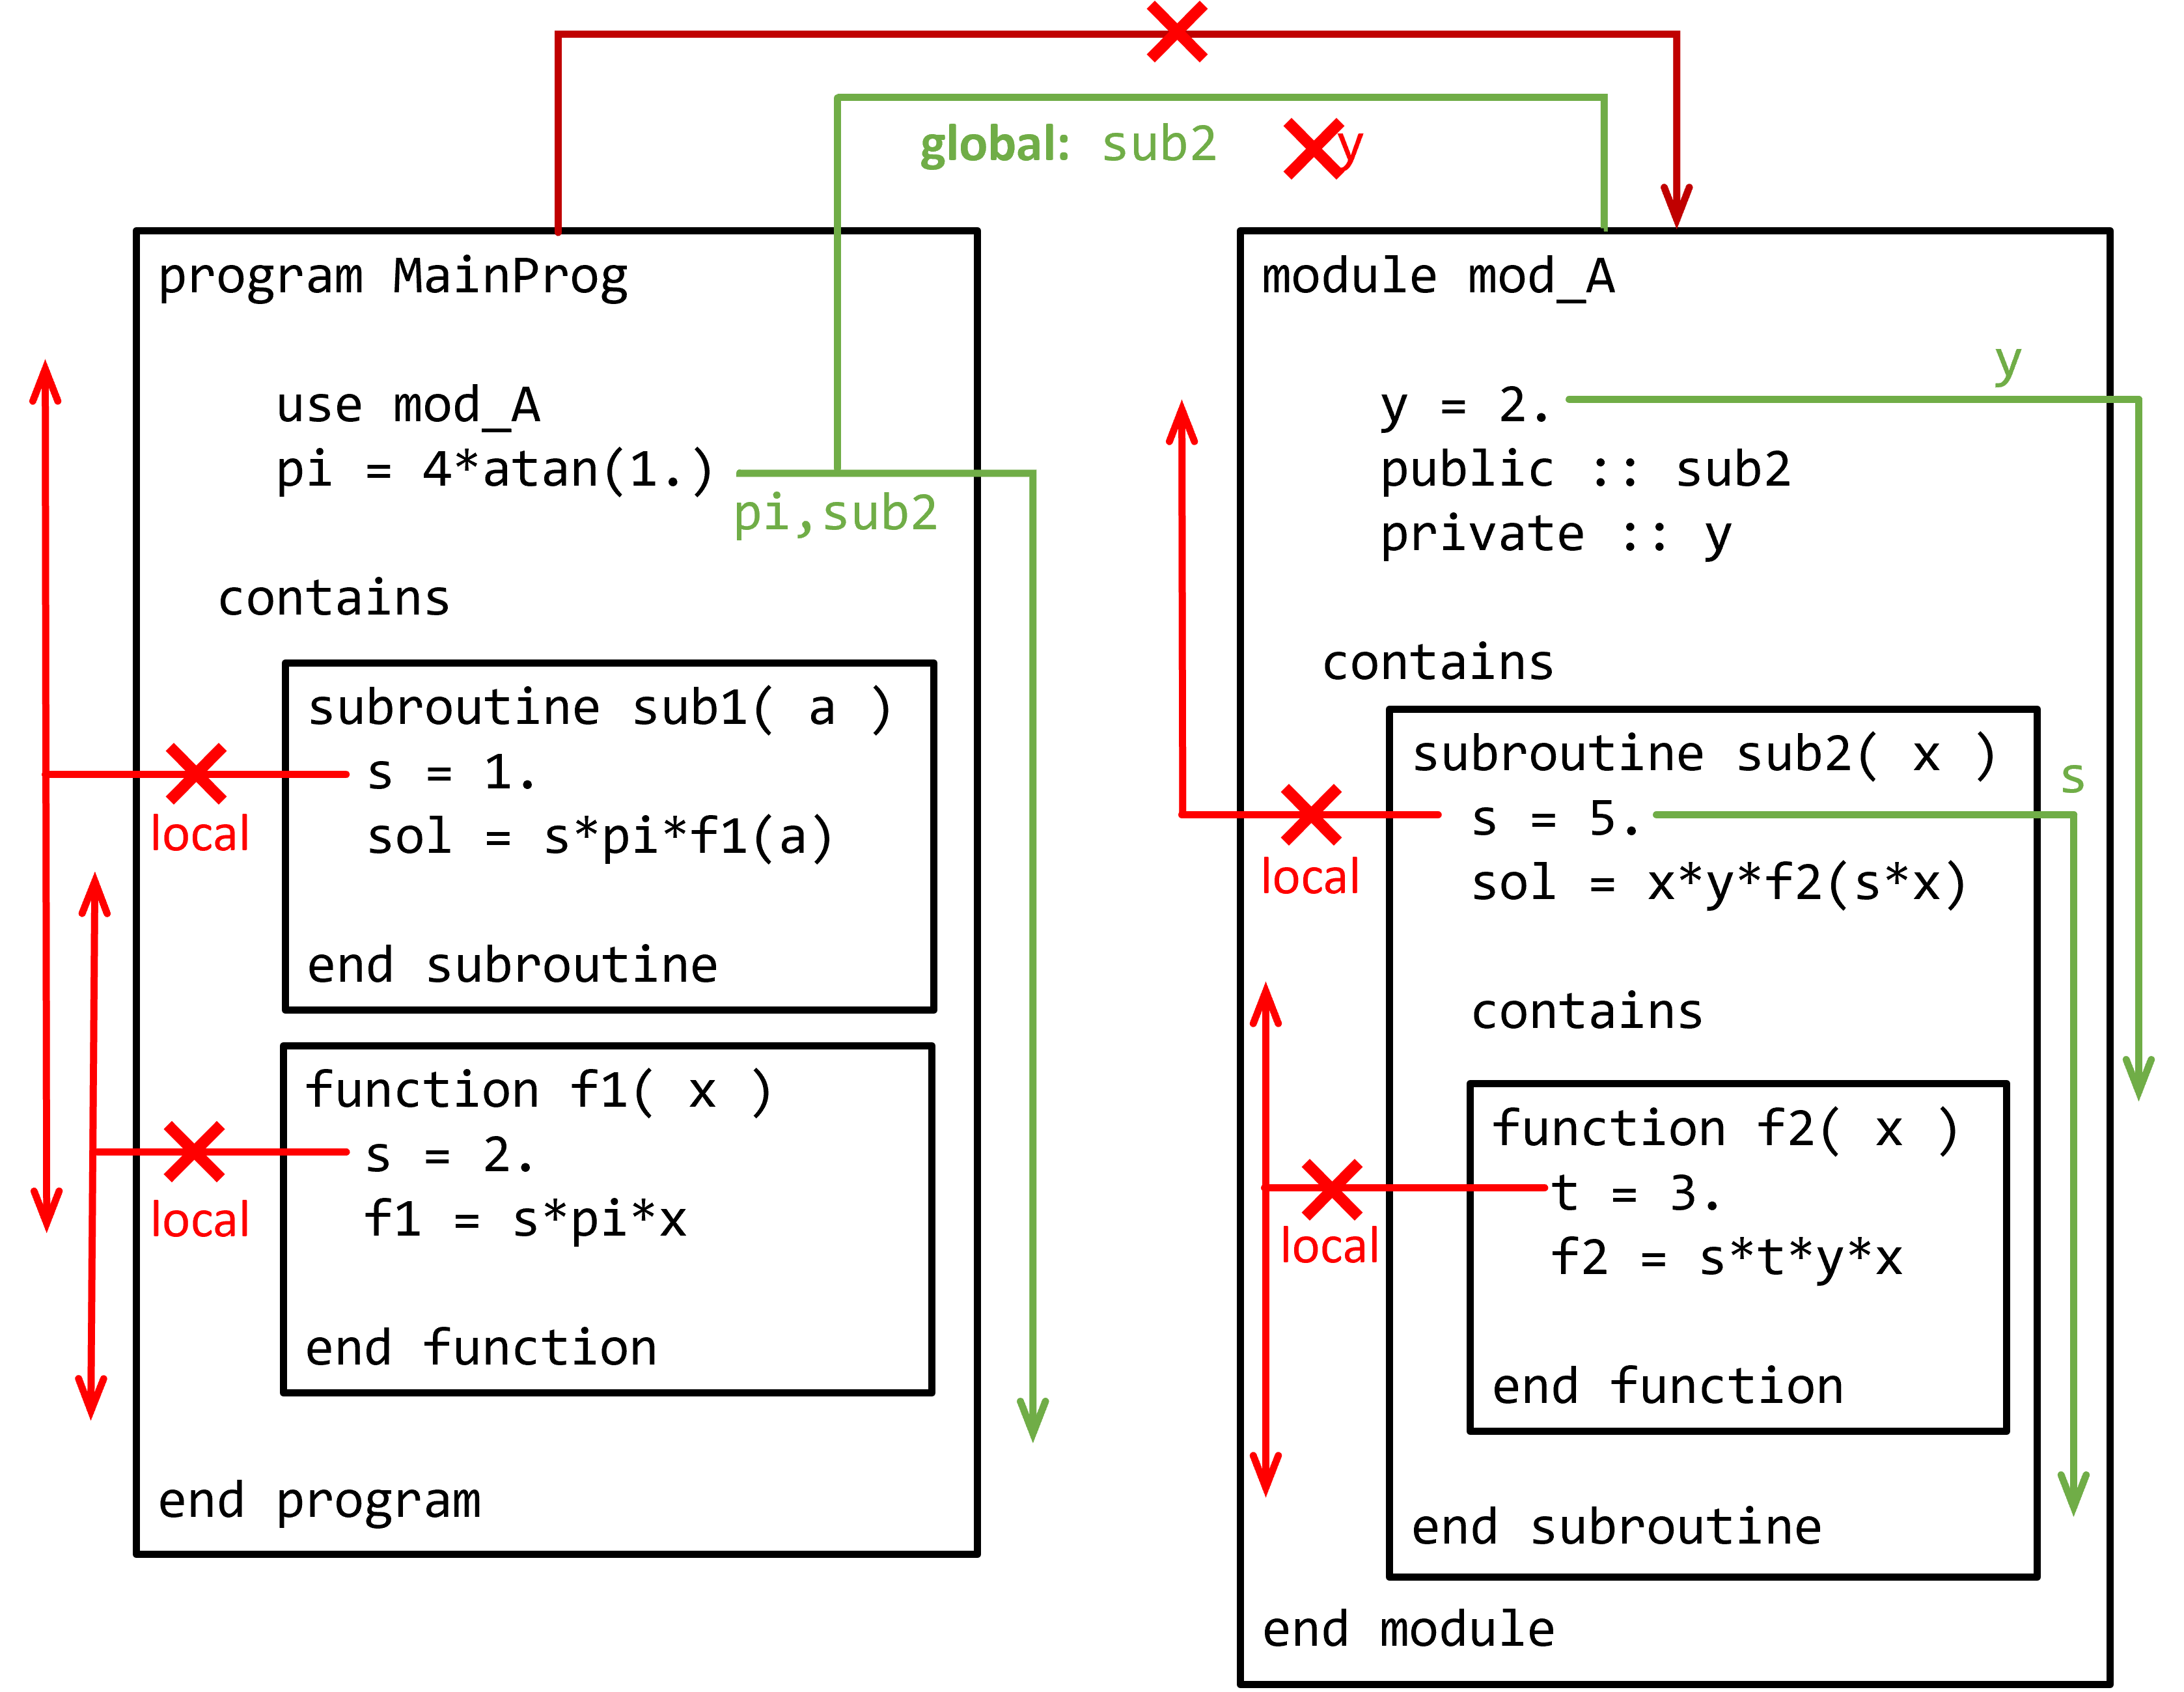
\includegraphics[width= \textwidth]{./doc/Figures/ScopeFor.png}
%    \caption{Example of scope for different variables and constants in both program units in Fortran. Notice that \texttt{MainProg} sees all entities of \texttt{mod\_A} by default, however, since \texttt{y} is declared as private, it won't be seen. Furthermore, function \texttt{f2( x )} is only accessible inside the subroutine \texttt{sub2( x )}, it won't be accessible from anywhere else. Finally, notice that \texttt{sub1( a )} sees \texttt{f1( x )} since both are global in the main program.}
%    \label{fig:ScopeFor}
%\end{figure}
%
%
%
%\begin{figure}[h]
%    \centering
%    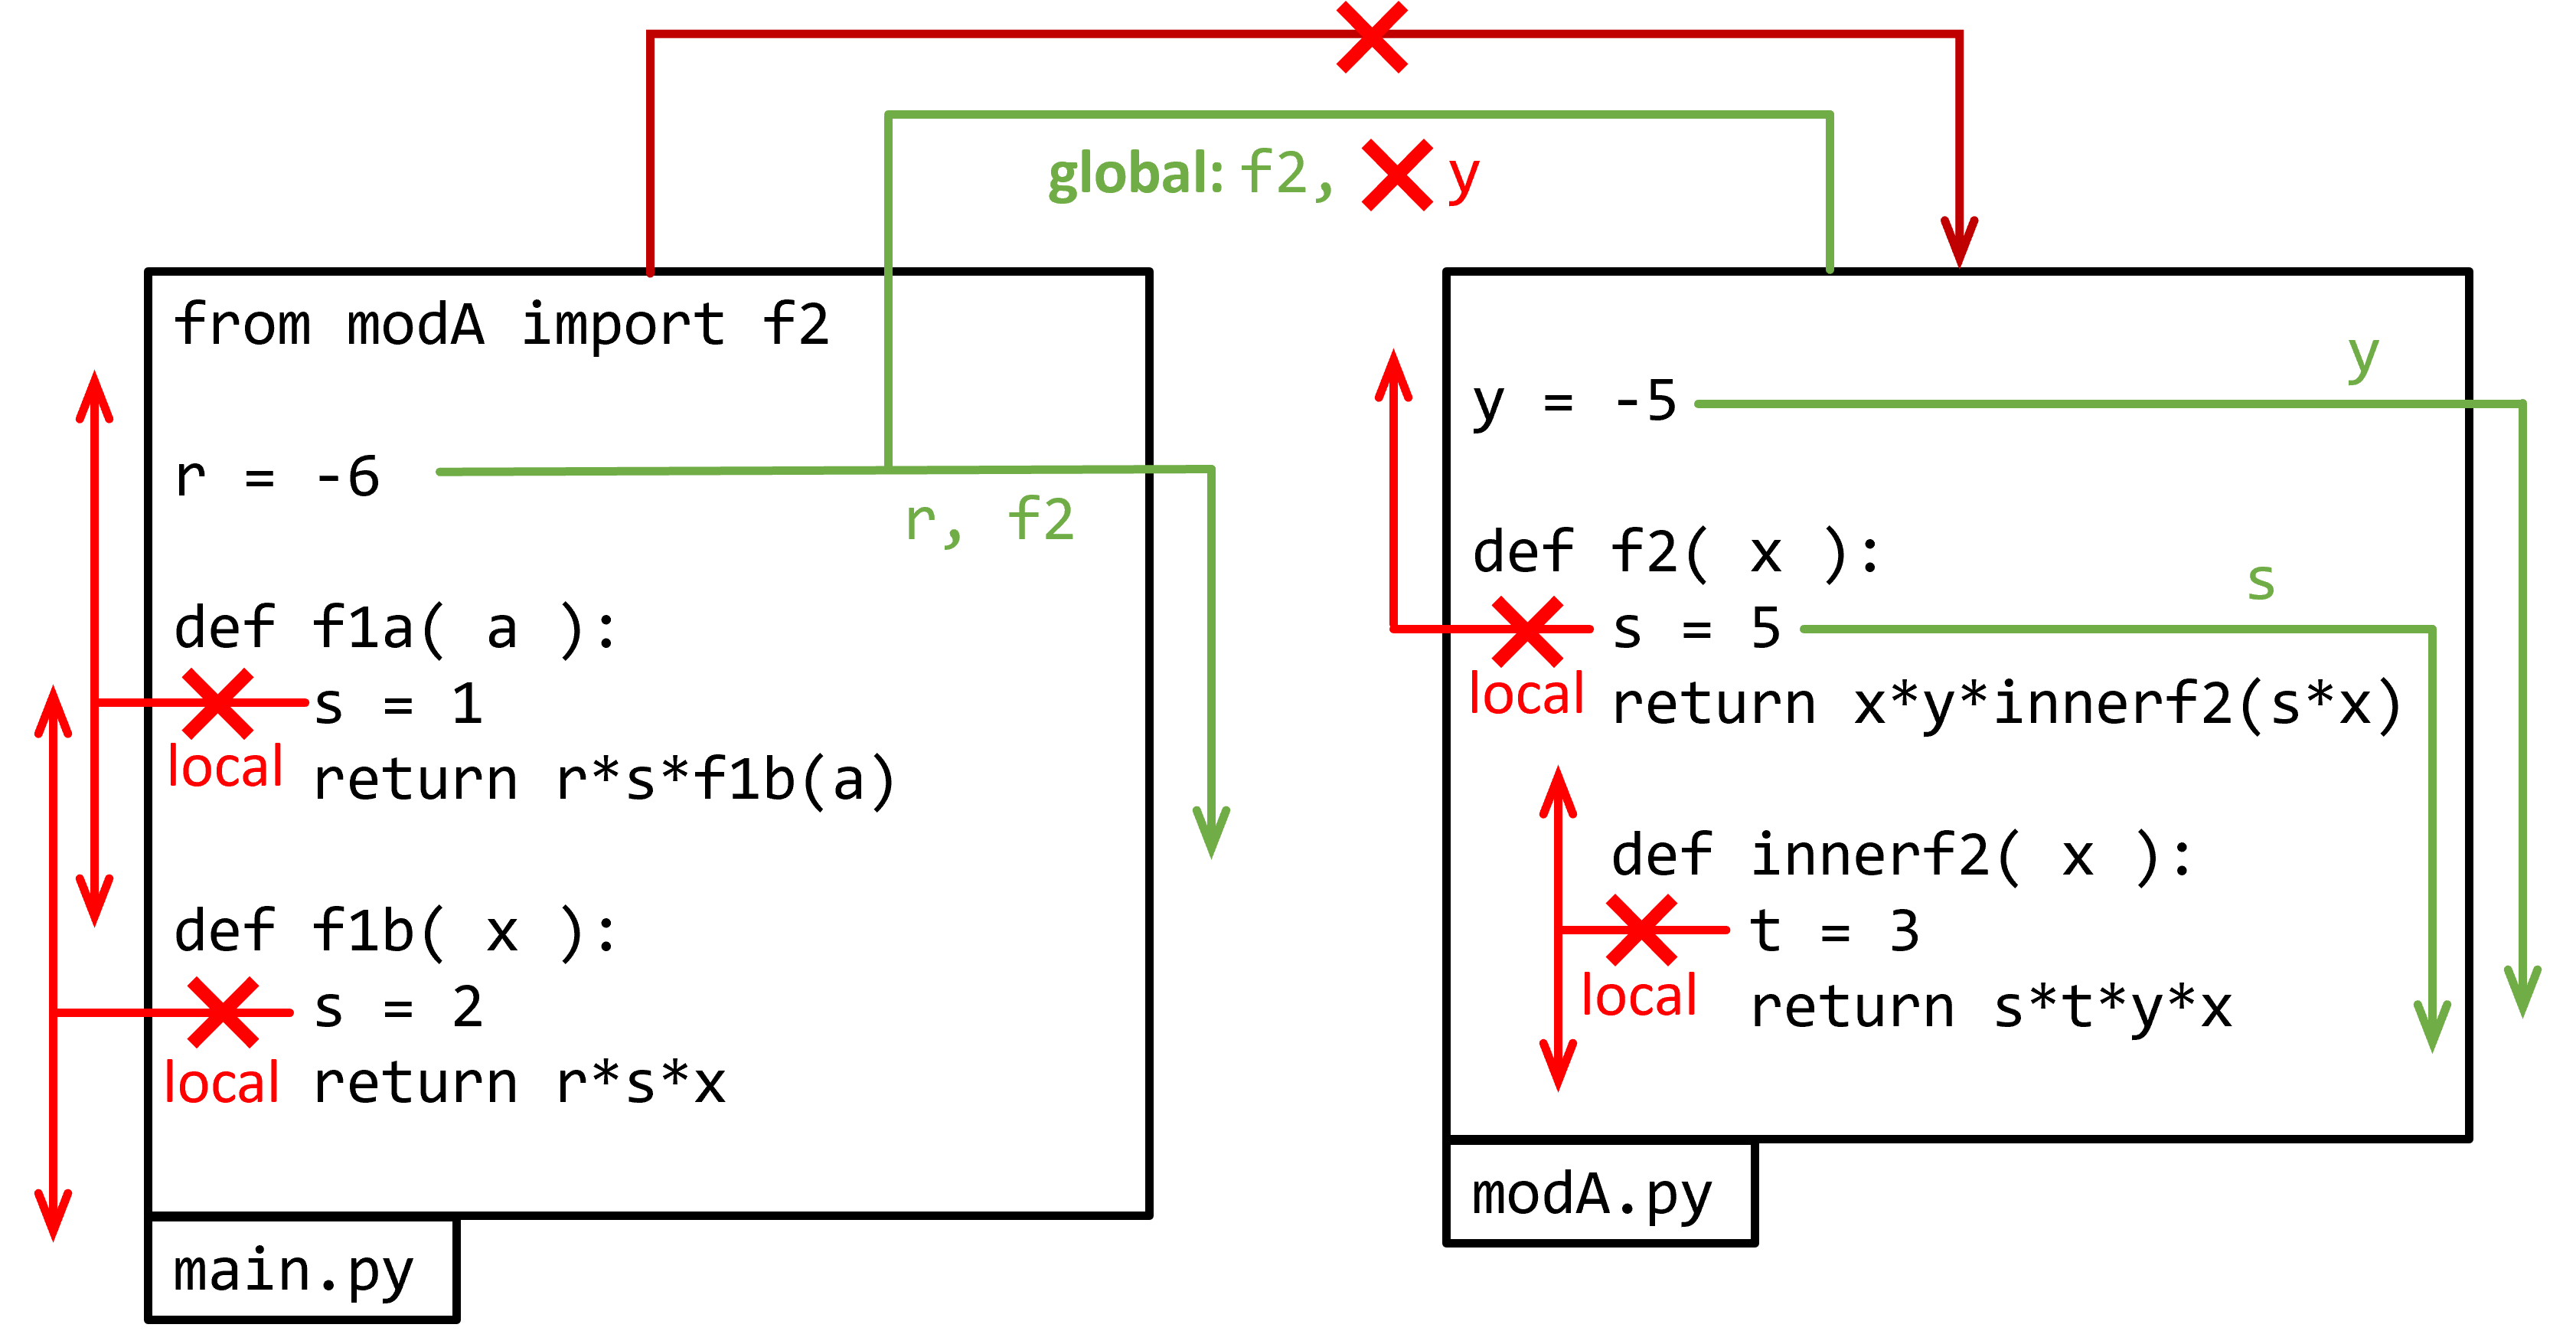
\includegraphics[width= \textwidth]{./doc/Figures/ScopePy.png}
%    \caption{Example of scope for different variables and constants in the main application and a module in Python. Notice \texttt{Main.py} sees only \texttt{f2( x )} from \texttt{modA.py} due to the selective import. In addition, function \texttt{innerf2( x )} is only accessible inside \texttt{f2( x )}, it won't be accessible from anywhere else.}
%    \label{fig:ScopePy}
%\end{figure}



%OLD
%The region of a program in which this variable or identifier is visible is called the scope.
%set of statements in which the variable can be used or modified
% This is called the scope of the visibility of some variable in some part of our code. 
%Local variables are those which specified inside the function or subroutine that we are dealing with and global variables are those that can be accessed by common variables of my own module  or by inclusions of other modules. 







  
       \chapter{Functional programming} 
\vspace{-1cm}
Functional programming is a programming paradigm 
to mimic mathematical functions. 
It can be considered a declarative programming language 
that builds complex functions by functional composition. 
Functional Programming is based on Lambda Calculus developed 
by Alonzo Church (1903-1995). 
Alan Turing (1912-1954), who was a student of Alonzo Church, created the 
universal Turing machine which laid the foundation of imperative 
programming style.
In 1957, Fortran language was created by John Backus(1924-2007).
In 1977, Backus described the Function Programming (FP) in his famous Turing Award lecture:
 "Can Programming Be Liberated from the von Neumann Style?".
%In the mid 1980s Backus and his colleagues came up with the language FL. 
%Python and Fortran both support functional programming in some degree.  
In this chapter, the following concepts, associated to functional 
programming paradigm, will be discussed through  different examples 
for Python and Fortran:  
\vspace{-0.25cm}
\begin{enumerate} 
 \setlength\itemsep{0cm}
\item First-Class functions.
\item Pure functions and side effects.
\item Recursion. 
\item Map, filter and reduce elemental functions.  
\item Modularity. 
%\item Closure.
\item Referential transparency. 
\end{enumerate} 
\vspace{-0.25cm}
Main advantages of functional programming are: its closeness 
to mathematical formulation, its ability to avoid side effects and 
its modularity to partition complex problems into easier ones.
One of main disadvantages is a lower  computational performance 
than imperative paradigm associated to recursion and functional composition
techniques.  Functional programming is usually used in mathematical 
computations and when parallelism or concurrency is required.


 
\newpage
 \section{First-class functions} 
A programming language has first-class functions 
when functions can be treated like any other variable. 
Namely, functions can be used in the following situations:  
\begin{enumerate} 
\item Function with arguments that are also functions.
\item Functions returning functions. 
\item Functions being assigned to other functions.
\end{enumerate} 

\subsection{Functions as arguments} 
Many mathematical concepts or functions are defined for a 
specific set of functions.
For example, the integral of some function is defined by: 
\begin{equation}
 I = \int _a ^b f(x)  \ dx, \qquad f: \mathbb{R} \rightarrow \mathbb{R}
\end{equation} 
It is desirable to implement a function to determine the definite integral
in the compact segment $ [a, b ]$ for any  
$  f: \mathbb{R} \rightarrow \mathbb{R} $. 
In order to have a complete example, an approximate method is needed to 
define the integral. Let's consider the right Riemann sum 
as an approximation by a finite sum: 
\begin{equation}
 I \approx \sum _{i=1} ^N f(x_i)  \ ( x_i - x_{i-1} ),
\end{equation}
where $ x_i $ is a partition of $ [a, b]$ 
\begin{equation}
 a = x_0 < x_1  < \cdots < x_N = b.
\end{equation}
In the following scheme, the interface of function integral is defined:  

\begin{center} 
 \begin{tikzpicture}
 \node[draw, fill=orange!20, minimum height=1.5cm, minimum width=3cm] (node) at (0,0) {Integral};
 \draw[->] (-2,0.35)node[anchor=east] {$a,b$} to (\tikztostart -| node.west);
 \draw[->, black] (-2,-0.35) node[anchor=east] {$f(x)$} to (\tikztostart -| node.west);
 \draw[->]  (1.5,0) node  {} to (2,0);
 \node[text width=1cm] at (2.7,0) {$I$};
 \end{tikzpicture}
\end{center} 



  
 \newpage 
  \subsubsection*{Fortran} 
The main purpose is to write a function with three arguments. The two first
are real numbers: $ a $ and $ b$. 
The interface definition of third argument  
$( f: \mathbb{R} \rightarrow \mathbb{R} ) $
is expressed with the following code:  
\vspace{0.5cm} 
   \renewcommand{\home}{./Fortran/sources/Advanced_programming/functional programming} 
   \lstfor
  \listings{\home/First_class_functions.f90}{abstract interface}
  {end interface}{First_class_functions.f90}
Once every argument is defined, the function integral is implemented: 
%  \listings{\home/First_class_functions.f90}{subroutine Function_examples}
%  {end subroutine}{First_class_functions.f90}
 \vspace{0.3cm}  
 % \newpage 
  \listings{\home/First_class_functions.f90}{real function Integral}
  {end function}{First_class_functions.f90}
Note that the third argument is a procedure function defined above. 
The following example creates a function $ h(x) $ to be integrated 
using the new function \verb|Integral|. 
 \vspace{0.3cm}  
  \listings{\home/First_class_functions.f90}{real function h}
   {end function}{First_class_functions.f90}
 
\newpage
\subsubsection*{Python}
Since Python is untyped language, 
\verb|Integral| function is implemented without specifying the type of its
arguments with the following code: 
\renewcommand{\home}{./Python/sources/Advanced_programming/functional programming}
\lstpython 
\vspace{0.5cm}
\listingsp{\home/First_class_functions.py}{def Integral}
  {return}{First_class_functions.py}
Note that the extension of the \verb|Integral| function has been reduced 
drastically by sacrificing 
the specifications or variables and arguments. 
Once someone makes use of this function, the Python interpreter will 
check dynamically that the operations involved in the above code 
are defined.
If the function $ h(x) $ is defined by: 
\vspace{0.5cm}
\listingsp{\home/First_class_functions.py}{def h}
  {return}{First_class_functions.py}
by invoking 
\vspace{0.5cm}
\listingsp{\home/First_class_functions.py}{R = Integral}
  {print}{First_class_functions.py}
will work without any problem.    

\newpage 
\subsection{Functions returning functions} 
In mathematics, 
function composition is an operation 
that takes two functions $f$ and $g$, and yields a function $ h = g  \circ  f  $ 
such that $ h(x) = g(f(x))$. 
Once the image of $ x $ is obtained by applying the function $ f $, 
a new image  $g(f(x))$ is yielded by applying $ g $. 

In Fortran language, functions can not return functions. 
The only possibility is to create derived types comprising 
functions or procedure pointers. This strategy is closer to the
Object Oriented Programming and it will treated in next chapters. 
However, Python allows very intuitively to build functions returning functions. 

\subsubsection*{Python}
The following example shows the definition of a function which returns 
the function composition of $ f $ and $ g $
\lstpython 
\vspace{0.5cm}
\listingsp{\home/First_class_functions.py}{def compose}
  {return h}{First_class_functions.py}
  
\subsection{Functions being assigned to other functions} 
Following with the same mathematical example, 
the creation of a new composition function is written in mathematical 
language as:
\begin{equation}
     h = f \circ g  
\end{equation} 
Fortran does not allow to assign functions to each other. 
The same strategy described above based on function or procedure pointer can be used to 
overcome this deficiency. However, Python allows to assign function
 as if they were variables as it is shown in the following code snippet: 
\lstpython 
\vspace{0.4cm}
\listingsp{\home/First_class_functions.py}{sqrt}
  {sqrt}{First_class_functions.py}




\newpage   
\section{Pure functions} 
In computer programming, a pure function is a function 
that returns values identical for identical arguments
and has no side effects. 
Hence, a pure function is a computational analogue of a mathematical function. 
Pure functions can be explicitly declared in Fortran with the \verb|pure| attribute.
However, in Python there is no way to force a function to be pure.  
The following list constitutes the requirements for a function to be pure.    
 \begin{enumerate}
  \setlength\itemsep{0.1cm}
 \item The function must not alter any dummy argument. 
 To accomplish that in Fortran,  arguments must have \verb|intent(in)| attribute 
 unless they are procedures or pointers.   
 \item The function must  not alter any part of a variable accessed by host or 
 use association. 
 \item Local variables can not have the \verb|SAVE| attribute(Fortran) or be saved. 
 \item Functions as arguments must be pure. 
 \item No external input/outputs operations are allowed. 
 \item STOP is not allowed. 
 \end{enumerate}   
If the Fortran function is declared with the \verb|pure| attribute and any of those 
requirements are not fulfilled, the compilation process of the source code will prompt an error.
In Python if pure functions are required, special care should be taken into account with these 
requirements. 
Those requirements are needed to assure that pure functions returns 
the same values for identical input arguments. 
One of main characteristics of any software development strategy is data hiding. It means that
non necessary data should be hidden to avoid bugs or improper behavior. 
However, when external data or global variables are needed, 
pure functions must not modify those variables. 

It seems that writing the entire code with pure functions would be our goal to improve 
efficiency in developing software. However, sometimes because a database should be modified 
or a random number generator is used, the same output is not obtained. 
The goal is to use pure functions when practical. Total purity 
is not practical but what about  80\% purity.


For sake of clarity, requirements to implement pure functions are  discussed in the following example: 
\newpage  
    \renewcommand{\home}{./Fortran/sources/Advanced_programming/functional programming} 
    \lstfor
   \listings{\home/First_class_functions.f90}{pure_functions}
   {end subroutine}{First_class_functions.f90}
The function \verb|f(x)| is declared to be pure. It has only one argument a real value \verb|x|.
As it was mentioned, \verb|x| must be specified with the \verb|intent(in)| attribute 
in order not to be modified accidentally.
A local variable \verb|b| is declared. This local variable can not have the \verb|SAVE| attribute
or can not be initialized to avoid undesirable historical effects. 
The function \verb|f_impure(x)| is impure because it has the initialization \verb|real::b=1|.
The first time this function is called with $ x=1$, it gives \verb|4,0| and the second time 
it yields \verb|5.0|. The reason is because the variable \verb|b| is only initialized at compilation 
time and saved for future calls. The first time \verb|f_impure(x)| is called, 
and after the sentence \verb|b=b+1|, variable \verb|b| holds \verb|2.0|. 
The second time \verb|f_impure(x)| is called, 
and after the sentence \verb|b=b+1|, variable \verb|b| holds \verb|3.0| and 
 \verb|f_impure(x)| gives a different value than the first call with identical input \verb|x|. 
Those are typical errors that can be avoided by writing  pure functions.

   


\newpage  
\section{Recursion}
\vspace{-0.5cm}  
In mathematics, a recursive definition or inductive definition, 
is used to define the elements in a set in terms of other elements in the set.
A recursive function is a function that its value at any point can be calculated 
from the values of the function at some previous points. 
For example,  the Fibonacci sequence 
\begin{equation} 
F(n) = F(n-1) + F(n-2)
\label{Fibonacci} 
\end{equation}
gives $ F(n) $ once $ F(n-1) $ and $F(n-2)$ are known. If the function values at  $n=0$  and 
$ n=1$ are known, the function value at $ n=2$ can be obtained from  the equation (\ref{Fibonacci}).
Recursive functions in programming languages allows to obtain the sequence 
from the declarative point of view. That is, it is not need to develop an iterative 
or imperative procedure as it is described above. 
As it was mentioned, recursive procedures are less efficient in terms of computational 
resources than iterative implementations. However, recursive implementations are easier to 
debug and to implement.  
 
\vspace{-0.5cm}
\subsection*{Fortran}
 \renewcommand{\home}{./Fortran/sources/Advanced_programming/functional programming} 
    \lstfor
   \listings{\home/First_class_functions.f90}{function Fibonacci}
   {end function}{First_class_functions.f90}
   \vspace{-0.8cm}
\subsection*{Python}
 \renewcommand{\home}{./Python/sources/Advanced_programming/functional programming} 
    \lstpython
   \listingsp{\home/First_class_functions.py}{def Fibonacci}
   {n-2}{First_class_functions.py}
   
   
 
  
\newpage  
\section{Map, filter and reduce}

In mathematics, mapping refers to the action of applying a function to the elements of its domain.
Mapping applies to any set: a collection of objects. 
\begin{equation} 
   f:A \rightarrow B 
\end{equation}    
is a map from $ A $ to $ B$; for every 
$ a $  in $ A$, there is a unique object $ f(a)$  in $ B$.
For example, rotating 
a body about a point is a map that transforms the body coordinates into new coordinates 
keeping the axes fixed. 



A filter tests each element of a set with a unary predicate. 
Elements that satisfy the predicate are kept and  those that don’t are removed. 
A filter on a set $ X $ is 
a subset  $ B \subseteq X $.


Reduce combines the elements of the set together using a binary function to get a scalar result. 
Examples of functions that perform reduction on arrays are: sum, product, all, any, minval,  maxval, maxloc
and minloc.



 
 


\vspace{1cm} 
\begin{IN}
The mathematical concepts: map/filter/reduce allow a software design 
simplifying the implementation of functions that operate over sequences of elements
enabling an implementation with no explicit control flow, not a single loop or if statements.
\end{IN}
\vspace{0.5cm} 
These mathematical concepts are taken into account in a functional programming language 
such as Python and Fortran and they will be explained in the following sections through examples.







\newpage 
\subsection{Mapping} 
To explain the implementation of the map functionality, let's consider a rotation 
which is a map of a plane into itself. The rotated coordinates of the point $(x,y)$ with an angle 
$\theta$ are: 
\begin{equation}
\begin{pmatrix}
x_r \\
y_r
\end{pmatrix}
=
\begin{pmatrix}
cos \ \theta & -sin \ \theta\\
sin \ \theta &  cos \ \theta
\end{pmatrix}
\begin{pmatrix}
x \\
y
\end{pmatrix}
\label{rotation} 
\end{equation} 
In the following example a square is rotated $ \pi/4 $ radians.
\subsubsection*{Fortran}
\renewcommand{\home}{./Fortran/sources/Advanced_programming/functional programming} 
  \lstfor
 \listings{\home/map_filter_reduce.f90}{type :: point2D}
 {end type}{map_filter_reduce.f90}
 \listings{\home/map_filter_reduce.f90}{function Rotation}
  {end function}{map_filter_reduce.f90}
\listings{\home/map_filter_reduce.f90}{image =}
  {imageR =}{map_filter_reduce.f90}  
First, the new type \verb|point2D| is defined. It is determined by its $ (x,y)$ coordinates. 
Then, rotation equation (\ref{rotation}) is implemented in \verb|Rotation|.
Finally, a set of  \verb|point2D| points is mapped with the \verb|Rotation| function which is written 
for a generic \verb|point2D| point. Note that the attribute \verb|elemental| of this function allows
to apply this functions for isolated elements or for a whole set of points. 

\subsubsection*{Python}
\renewcommand{\home}{./Python/sources/Advanced_programming/functional programming}
 \lstpython
 \listingsp{\home/map_filter_reduce.py}{def Rotation}
  {return}{map_filter_reduce.py}
  \vspace{0.5cm} 
\listingsp{\home/map_filter_reduce.py}{image =}
  {imageR =}{map_filter_reduce.py}  
Since Python is an untyped langauage, there is no need to define the plane point \verb|P|.
Hence,  \verb|Rotation| function is implemented assuming that \verb|P| is an numpy array with 
two components. This is assumed from expression \verb|matmul(A, P)|. 
Since \verb|A| is a square matrix of dimension 2, \verb|P| should be a vector of dimension 2 
 to have a conformal operation. 
 
Finally, a set of points is mapped with the \verb|Rotation| function which is written 
for a generic point. Note that the keyword \verb|map| allows this mapping. 
The first argument of \verb|map| is the scalar function to be applied to each element 
of the set and the second argument is the set. Since \verb|Rotation| has two arguments: 
point and angle to be rotated, a \verb|lambda| function is used to define a 
new function with only one argument.  



  
  
 \newpage 
\subsection{Filter and reduce} 
In Fortran, filtering is accomplishing by the intrinsic function \verb|pack| and
reduce operation with different functions. In this example, \verb|minloc| is used.   
A set of random two dimensional points is generated 
in the square $ [-1, 1] \times [-1,1]$.  This set of points is filtered through the \verb|filter|
function which determines if the point is inside the region enclosed between
the two concentric circles of radius \verb|R1| and \verb|R2|. Since the function \verb|filter|
has \verb|elemental| attribute, the statement \verb|filter(set, 0.4, 0.7)| constitutes 
a mapping for all elements of \verb|set|. The intrinsic function \verb|pack|
filters the complete \verb|set| yielding a \verb|subset|. Finally, \verb|minloc| is used 
as an example of reduce functions. 

\vspace{-0.5cm}
  \subsection*{Fortran} 
  \renewcommand{\home}{./Fortran/sources/Advanced_programming/functional programming} 
   \lstfor
  \listings{\home/map_filter_reduce.f90}{subroutine test_filter_reduce}
  {Nearest}{map_filter_reduce.f90}
   
  \listings{\home/map_filter_reduce.f90}{function filter}
  {end function}{map_filter_reduce.f90}
  
  
\newpage 
\subsection*{Python}
In Python, filtering is accomplishing by the intrinsic function \verb|filter| and
reduce operation with different functions. In this example, \verb|armin| is used.   
A set of random two dimensional points is generated 
in the square $ [-1, 1] \times [-1,1]$.  
This set of points is filtered through the \verb|filter_d|
function which determines if the point is inside the region enclosed between
the two concentric circles of radius \verb|R1| and \verb|R2|. Since the function \verb|filter_d|
has three arguments, a lambda function is used to meet the requirement of the first a argument 
of the function \verb|map|. The result of \verb|filter| is transformed a list and later to a
numpy array.  Finally, \verb|argmin| is used 
as an example of reduce functions.  
  
\vspace{0.5cm}   
  \renewcommand{\home}{./Python/sources/Advanced_programming/functional programming}
  \lstpython
  \listingsp{\home/map_filter_reduce.py}{def test_filter_reduce}
  {Nearest}{map_filter_reduce.py}
  \listingsp{\home/map_filter_reduce.py}{def filter_d}
  {return}{map_filter_reduce.py}
   \listingsp{\home/map_filter_reduce.py}{distance}
    {return}{map_filter_reduce.py}
  
  
  
 \newpage 
 \subsection*{Fortran} 
 In this last example, an array of char strings
 containing numbers  is transformed to an array numbers by means of a mapping. 
 Then, the array is filtered (\verb|pack|) retaining only those elements which are greater than 
 200 and, finally, a reduce function \verb|maxval| is used  to obtain the maximum value of the 
 array. 
 \vspace{0.5cm}
 \renewcommand{\home}{./Fortran/sources/Advanced_programming/functional programming} 
  \lstfor
 \listings{\home/map_filter_reduce.f90}{subroutine test_map_filter_reduce}
 {end subroutine}{map_filter_reduce.f90}
  \vspace{0.5cm}
 \listings{\home/map_filter_reduce.f90}{elemental integer function str_to_number}
 {end function}{map_filter_reduce.f90}
 
 
\newpage 
\subsection*{Python}
In this last example, a list  of char strings
containing numbers is transformed to a list of numbers by the \verb|map| function. 
Then, the list is filtered (\verb|filter|) with \verb|my_filter| predicate
retaining only those elements which are greater than 
200 and, finally, a reduce function \verb|max| is used to obtain the maximum value of the 
list. 
 \vspace{0.5cm}
 \renewcommand{\home}{./Python/sources/Advanced_programming/functional programming}
 \lstpython
 \listingsp{\home/map_filter_reduce.py}{def test_map_filter_reduce}
 {max value}{map_filter_reduce.py}
 \vspace{0.5cm}
 \listingsp{\home/map_filter_reduce.py}{def str_to_number}
 {return}{map_filter_reduce.py}
 \vspace{0.5cm}
 \listingsp{\home/map_filter_reduce.py}{def my_filter}
  {return}{map_filter_reduce.py}
 
 
\newpage   
\section{Modularity} 
Modular programming is a software design technique that separates 
the functionality of a program into independent modules containing 
specific aspects  of the required functionality.
Modular programming developed in the late 1960s and 1970s, 
as a larger-scale analog of the concept of structured programming (1960s).
Structured programming was developed to improve the clarity of a computer 
program by making use of the structured control flow sentences (if/then/else, while/for).
Modular programming  refers to the high-level decomposition of the code 
and structured programming refers 
to the low-level code use of structured control flow.

Python and Fortran allows to develop huge programs based on different modules.
In Python,  modules are source Python files containing functions that 
can be imported or used easily from another Python file. It can be considered a Python library. 
In Fortran, modules are specified by the name \verb|module xxx| and they can be stored in Fortran
source files. To follow the same methodology than Python, it is advisable to name that 
Fortran source file with same name  than the module storing only one module per file. This 
Fortran file \verb|contains| functions. 
Since Python is an untyped language, interface of functions is unknown when imported. 
This is a double-edge sword. The favorable consequence is the same function could be used 
for different data types if the involved operations are defined. The bad consequence is that 
errors associated to wrong use of the functions are only detected at run time. 
On the contrary, Fortran has explicit interface of all public functions contained in some module 
when it is used. This explicit interface allows to correct 
implementing errors at compiling time. However, overloading is needed when 
calling those functions with new types. 
In both languages, modularity is a pillar in functional programming creating 
abstractions in a hierarchical fashion.

For example, to solve a nonlinear system of partial differential equations, 
the following layers or modules can be defined: 
\begin{enumerate}
\setlength\itemsep{0cm}
\item Application layer: solve a nonlinear system of partial differential equation. 
\item Discretization layer: discretization method for partial differential equations.  
\item Non linear solver: functions to solve nonlinear system of equations 
such as Newton method.
\item Linear algebra:  methods to solve linear systems of equations. 
\end{enumerate}
The original complex problem is formulated by functional composition into smaller
or simpler problems or functions. 
One of the main goals of modularity in functional programming is the ability to 
build different methods of different modules without knowing the functionality of 
other modules. Besides, an extra effort must be put to define the hierarchical 
structure.  


 

 
 
  
%\newpage  
%\section{Closure} 
%
% 
% \newpage 
%  \renewcommand{\home}{./Fortran/sources/Advanced_programming/functional programming} 
%  \listings{\home/First_class_functions.f90}{real function Moment}
%  {end function}{First_class_functions.f90}
%  
%
% and lexical scoping
%
%
%Lexical scoping defines how variables are seen in nested functions.
%When functions are defined inside other functions, the scope of this inner 
%function comprises local variables of the actual function and 
%local variables of those outer or parent functions.
%
%
% 
%inner functions contain the scope 
%of parent functions even if the parent function has returned.
% 


\newpage  
\section{Referential transparency}  
In functional programming, referential transparency is defined as the fact that a 
math expression involving function evaluations can be
simplified or rewrite in different order without changing the result of the program.
The concept was originated in Alfred North Whitehead and 
Bertrand Russell's Principia Mathematica (1910–13).
Mathematical concepts, such as simplification or factorization applies also
to functional programming. Imagine, for example, the following math expression: 
\begin{equation}
g(x) + g(x) \ ( h(x) - 1 ). 
\end{equation} 
By extracting the common factor $ g(x) $, the expression simplifies to yield: 
\begin{equation}
 g(x) \  h(x). 
\end{equation} 
This is always true for mathematical functions. However, 
when trying to simplify expressions in a programming code, it is only valid when dealing 
with pure functions. 
Imagine the following example with  $ g(x) $ impure: 
 \vspace{0.5cm}
 \renewcommand{\home}{./Fortran/sources/Advanced_programming/functional programming} 
  \lstfor
  \listings{\home/First_class_functions.f90}{referential_transparency}
 {end function}{First_class_functions.f90}
Every time $ g(x) $ is evaluated, the statement \verb|b=b+1| increases by one the 
\verb|b| variable
yielding different values of $ g(x)$ for identical values of its argument $x$ 
($g(x)$ is an impure function). 
In this example, the first expressions gives \verb|3.0| and the simplified expression 
gives  \verb|5.0|. It is said tha the above expression is not referentially transparent 
and this simplification is not allowed or gives different results. 
Referential transparency is desirable property 
to factorize or simplify programming codes. 
%To attain referential transparency, all functions and procedures 
%should be pure.  
If all functions involved in some expression are pure functions, 
then the expression is referentially transparent.


\newpage
\subsection{Benefits of referential transparency} 
When developing huge numerical codes, specifications are not always perfectly clear. 
Final specifications usually evolve with results of different tests. Besides, it is very easy to 
write impure functions when external or global variables are needed.
Math abstractions are explored and defined at the same time or after the code is functional. 
Additionally,  when different developers are involved,  
similar or repetitive functions are written making grow the code unnecessarily. 
All these issues usually originate  huge codes that should be 
rewritten to yield: robust, easy to maintain, more efficient and fast codes. 
From the point of view of the authors, these issues eventually originate 
the following three categories of programming code: 
\begin{enumerate}
\item Spaghetti code. Usually, imperative programming dominates the scenario. 
\item Encapsulated code. Some effort is put in functions isolation but a real hierarchical 
 structure is missing. 
\item Multilayer code. Simple math abstractions are encapsulated in pure functions and 
more complex functions are built by function composition of pure functions. 
\end{enumerate}
The main benefit of referential transparency  is
the ability to read, understand, reason about and modify our 
functions without altering the external world. 
When the code is written with pure functions, different developers are able to write 
their pure functions without knowing the code of other programmers or other layers. 
Even if they need the outputs of some layers that are not written yet, the referential
transparency allows to substitute these functions by emulators that gives
the value it is supposed to yield. 


Functional programming  with referential transparency or pure functions allows to rewrite and reorder 
a huge programming code easier than imperative programming. 
The semantics of an imperative programming language is based on definition 
and ordering of different sequence points.
If the substitution of an expression with its value is valid only at a certain point 
in the execution of the program, then the expression is 
not referentially transparent. 
However, pure functional programming 
is referentially transparent and expressions can be evaluated at any time. 
Hence, there is no need to define sequence points and no need 
to guarantee of the order of evaluation. 
This advantage allows to test the code with compilers or to refactor
the code with intelligent tools. 

Other benefits of referential transparency is refactoring and maintenance tasks. 
Huge numerical programming codes are always evolving by including new functionalities 
or by improving theirs performances. 

  
%\newpage  
%\section{Monads}   
       
       
\chapter{Overloading functions and operators}    \label{ch:overloading}
From the mathematical point of view operators and functions representing 
common concepts can be to different types of different n-dimensional spaces.
It is desirable to maintain the same operators or the same function names 
by overloading function names and operator symbols. 
If the programming language is a compiling language, such as Fortran, 
the compiler identifies, at compilation time, the type of the operands or the arguments 
involved when calling a function and it selects automatically the proper operation. 
If the language is untyped interpreted language, such as Python, overloading is not supported. 
However, there are many alternatives to emulate overloading in Python. 

Operators can be applied to elements of sets with different types.
For example, the operator \texttt{+} 
is defined differently for real numbers of complex numbers. However, the same operator 
is used for those different operations. This is done by overloading the operator. 
If $x$ and $y$ are reals, the expression $ x+y $ involves the operator \texttt{+}
which is the classical sum. 
However, if  $u$ and $v$ are complexes, 
the expression $ u+v $ involves the same operator \texttt{+}. It this case, 
the result yields a complex number in which 
the real part is the sum of real parts of $ u $ and $ v $
and the imaginary part is the sum of imaginary parts of $ u $ and $ v $.
Many operands and functions are previously overloaded by the native language.

Additionally to operators, functions can also be overloaded. 
Functions are overloaded with n-dimensional spaces. 
For example, the mathematical concept: integral 
can be defined and overloaded for line integrals or surface integrals. 
 

\newpage 
\section{Overloading functions in n-dimensional spaces}

In this example, the function \texttt{Integral} is created to overload line integrals 
and surface integrals. 
Let's consider the  line integral in a compact segment $[a, b]$: 
\begin{equation}   
    I =  \int _a ^b f(x) \ dx, \qquad f: \mathbb{R} \rightarrow \mathbb{R},   
\end{equation} 
and the surface integral in a compact square $ \Omega = [a, b] \times [c,d]$:   
\begin{equation}   
    I =  \int _{\partial \Omega} f(x, y) \ dx \ dy, 
    \qquad f: \mathbb{R}\times \mathbb{R} \rightarrow \mathbb{R}.   
\end{equation} 
From the software point of view, using the same word \texttt{Integral}
to invoke surface or line integrals is desirable. 
Besides, a surface integral can be expressed by the following way: 
\begin{equation}   
    I =  \int _{a} ^b \left(   \int _{c} ^d f(x,y) \ dy      \right) \ dx,
\end{equation} 
in which the integrand is defined with the parametric line integral:
\begin{equation}   
   I_1(x) = \int _{c} ^d f(x,y) \ dy.  
   \label{I1}   
\end{equation} 
The final expression for the surface integral is:  
\begin{equation}   
    I =   \int _{a} ^b I_1(x) \ dx. 
    \label{I2D}  
\end{equation} 
Hence, a surface integral can be defined by functional composition of line integrals. 
In the expression,  $ I_1(x) $, the variable $ x $ acts as a parameter
and $ I_1(x) $ is calculated by means a line integral. 
 
In the following pages, these two concepts overloading and functional composition
are taken into account to write two implementations in Fortran and Python. 

 
\newpage  
\subsection*{Fortran}

\renewcommand{\home}{./Fortran/sources/Advanced_programming/overloading} 
\lstfor

First, the overloading implementation is explained. Once two different functions are 
created for line and surface integrals, the overloading implementation is done
with the following code: 
\vspace{0.5cm}  
\listings{\home/overloading.f90}{interface Integral}{end interface}{overloading.f90}
At compilation time, function invocations are analyzed ans its proper function
is identified. In the following code, two integrals are invoked with 
different number and type of arguments.
\vspace{0.5cm} 
\listings{\home/overloading.f90}{subroutine test_Integral}{end subroutine}{overloading.f90}
The first \texttt{Integral} invocation has three arguments, the two first are reals and the 
third \texttt{f1} is a real function.
The second \texttt{Integral} invocation has five arguments, the four first are reals and 
the fith \texttt{f2} is a real function 
$(\mathbb{R}\times \mathbb{R} \rightarrow \mathbb{R})$.
What rest is to write, \texttt{Integral1D} and \texttt{Integral2D} accoding to their 
specifications.  
\newpage  

Let's begin with  \verb|Integral1D| implementation. 
Even though the numerical method to approximate the line integral is not relevant, 
a Riemann approximation is shown in the following code to have a complete testing
example that could be used as a template. 
\vspace{0.5cm} 
\listings{\home/overloading.f90}{function Integral1D}{end function}{overloading.f90} 
Note that the third argument is defined as a \verb|f_R_R| procedure or function. 
Hence, the definitions of \verb|f_R_R| for line integrals and \verb|f_R2_R|
for surface integrals are given in the following code: 
\vspace{0.5cm} 
\listings{\home/overloading.f90}{abstract interface}{end interface}{overloading.f90} 
 
\newpage  
Let's finish with \verb|Integral2D| implementation. 
Taking into account the definition of a surface integral expressed 
by  equations (\ref{I2D}) and (\ref{I1}), the following implementation is clear: 

\vspace{0.5cm}  
\listings{\home/overloading.f90}{function Integral2D}{end function}{overloading.f90} 
\verb|Integral2D|  is built by a line integral (\verb|Integral1D|) 
in which the integrand is parametric line integral defined by: 
\vspace{0.5cm}   
\listings{\home/overloading.f90}{function Parametric_I1D}{end function}{overloading.f90} 
    
 
 
\newpage
\subsection*{Python}
\renewcommand{\home}{./Python/sources/Advanced_programming/overloading}
\lstpython 
The same concepts are applied to implement an overloaded \verb|Integral| in Python. 
As it is mentioned repetitively, Python allows writing shorter codes 
than Fortran but paying the price of no specifying function arguments or variables. 


Even though Python does not allow overloading, an easy proposa  is shown to 
emulate overloading in the following code: 
\vspace{0.5cm} 
\listingsp{\home/overloading.py}{def Integral }{None}{overloading.py} 
At execution time, the \verb|Integral| function 
checks how may arguments are present. If the invocation is done with three
arguments, line integral is assumed. 
 If the invocation is done with five
arguments, surface integral is assumed. Otherwise, \verb|Integral| function
will show an error.  

In the following code, an example of the overloaded  \verb|Integral| is shown: 
\vspace{0.5cm}
\listingsp{\home/overloading.py}{def test_Integral}{y}{overloading.py}
Note that the first invocation has three arguments and the second invocation has five 
arguments. Note also that anonymous functions or lambda functions have been 
expressed in the last argument to make the example more compact.  


\newpage
Finallly, \verb|Integral1D| and \verb|Integral2D| ae implemented according to their
definitions.
\verb|Integral1D| is approximated by Riemann sums 
\vspace{0.5cm}
\listingsp{\home/overloading.py}{def Integral1D}{return}{overloading.py}

And \verb|Integral2D| is expressed by means of \verb|Integral1D| function 
according to its definition given by (\ref{I2D}) and (\ref{I1}). 
\vspace{0.5cm}
\listingsp{\home/overloading.py}{def Integral2D}{a, b, I1}{overloading.py}



\newpage 
\section{Overloading functions with complex numbers}

In this example, an ordinary differential system of equations is integrated
in real variable and complex variable. 
Let's consider the first order 
differential system of equations of dimension $ N $ in real variable: 
\begin{equation}   
    \frac{dU }{ dt} =  F( U,t ) , \qquad 
    F: \mathbb{R}^N \times \mathbb{R} \rightarrow \mathbb{R}^N,   
    \label{cauchy}
\end{equation} 
where $ U(t) \in \mathbb{R}^N $. This system of equations together with 
the initial condition $ U_0 $ constitutes a Cauchy problem and allows 
to determine the solution $ U(t) $ for all $ t \in [0, T]$.
To approximate numerically the solution of the Cauchy problem, a partition of
the time segment $ [0, T] $ is considered. 
Once this partition is defined by different time steps $ t_n $, the solution 
can be approximated by any temporal scheme. 
The Euler scheme is the easiest numerical method to approximate numerically 
the solution $ U^{n+1} $ at time step $t_{n+1} $ from the solution 
$ U^{n} $ at time step $t_{n} $. 
\begin{equation}   
    U^{n+1}=  U^n + \Delta t \ F( U^n, t_n), \qquad 
    n=0, \ldots, N  
    \label{euler}   
\end{equation}
In this example, 
the harmonic oscillator ($ \ddot x   + x = 0 $)  is integrated.
This oscillator can be formulated as a first order system of two equations:
\begin{equation}   
    \frac{d}{dt }   
 \begin{pmatrix}
 x \\
 \dot x
 \end{pmatrix}   
    = 
  \begin{pmatrix}
  \dot x \\
  - x
  \end{pmatrix}
  \label{oscillator}
\end{equation}
where the state vector can be  defined with $ U = ( x, \ \dot x  )^T $ 
and, consequently,  $ F= ( U_2, \ -U_1  )^T $. The same harmonic oscillator
can be expressed in complex variable by doing  $ Z = x + i \ \dot x  $. 
In complex variable, the equations of the harmonic oscillator yields: 
\begin{equation}   
    \frac{dZ}{dt }  = - i \ Z.
    \label{coscillator}
\end{equation} 
The main objective of this section is to show different alternatives 
to integrate in complex variable by means of functions written for 
real variable. 

Since Python is untyped, a minor modification will allow to integrate 
in real or in complex variable with the same functions.
On the contrary, Fortran variables are obliged to be typed.  
In this case, instead of writing new software to overload the Euler 
scheme, a different approach will be shown. The real function $ F $ in equation
(\ref{cauchy}) will be build by means of the complex function of equation
(\ref{coscillator}) and the complex system of equations will be integrated in real 
variable with minor modifications. 

In the following pages, these ideas will be developed 
to write two implementations in Fortran and Python. 

 
\newpage  
\subsection*{Fortran}
First, the \verb|Euler| function 
is implemented for real variable. Given an approximate solution \verb|U1| 
at time step \verb|t1|, the solution \verb|U2| at  time step  \verb|t2| 
is calculated by (\ref{euler}). 
\vspace{0.4cm}  
\renewcommand{\home}{./Fortran/sources/Advanced_programming/polymorphism} 
\lstfor
\listings{\home/polymorphic_ODES.f90}{function Euler}{end function}{polymorphic_ODES.f90}
Then, the real function of the harmonic oscillator (\ref{oscillator}) is defined by:
\vspace{0.4cm} 
\listings{\home/polymorphic_ODES.f90}{function oscillator}{end function}{polymorphic_ODES.f90}
Finally, a loop allows to calculate and to store every time 
step of the time partition. The matrix \verb|U(0:N,Nv)| holds \verb|N+1|
time steps for every \verb|Nv| variables. 
\vspace{0.4cm} 
\listings{\home/polymorphic_ODES.f90}{simulation}{end do}{polymorphic_ODES.f90}


\newpage 
To integrate the complex system, 
the harmonic oscillator equations (\ref{coscillator}) written in complex 
variable are implement with the following function: 
\vspace{0.4cm} 
\listings{\home/polymorphic_ODES.f90}{complex_oscillator}{end function}{polymorphic_ODES.f90}
Finally, the function \verb|complex_simulation| is built with complex 
arguments. It defines a real function \verb|F| which is created 
by means of the complex function \verb|Fc| and then 
the problem can be simulated in real variable. 
\vspace{0.4cm} 
\listings{\home/polymorphic_ODES.f90}{complex_simulation}{end subroutine}{polymorphic_ODES.f90}

 
\newpage
\subsection*{Python}
As it was mentioned, to overload the Python code to integrate a complex problem 
is much easier because Python functions are implemented without knowing 
the type of variables. 
First, the \verb|Euler| function 
is implemented. Given an approximate solution \verb|U1| 
at time step \verb|t1|, the solution \verb|U2| at  time step  \verb|t2| 
is calculated by (\ref{euler}).
\vspace{0.4cm} 
\renewcommand{\home}{./Python/sources/Advanced_programming/polymorphism}
\lstpython 
\listingsp{\home/polymorphic_ODES.py}{def Euler}{return}{polymorphic_ODES.py.py}  
Then, the real function of the harmonic oscillator (\ref{oscillator}) is defined by:
\vspace{0.4cm} 
\listingsp{\home/polymorphic_ODES.py}{def oscillator}{return}{polymorphic_ODES.py}
Finally, a loop allows to calculate and to store every time 
step of the time partition. The matrix \verb|U(0:N,Nv)| holds \verb|N+1|
time steps for every \verb|Nv| variables. 
\vspace{0.4cm} 
\listingsp{\home/polymorphic_ODES.py}{def simulation}{Euler}{polymorphic_ODES.py}
To integrate the system in complex variable, 
the complex function of the harmonic oscillator (\ref{coscillator}) is defined by:
\vspace{0.4cm} 
\listingsp{\home/polymorphic_ODES.py}{def complex_oscillator}{return}{polymorphic_ODES.py}
\newpage 
In the following code, the harmonic oscillator is integrated in real and in complex variable with the same 
code: 
\vspace{0.5cm} 
\listingsp{\home/polymorphic_ODES.py}{def complex_ODES}{complex_oscillator}{polymorphic_ODES.py} 
Note that while \verb|U0| is a nump array of real components, \verb|Z0| is a complex variable holding the 
same initial condition than \verb|U0|. 
The key idea of this overloading is hidden in the function \verb|simulation|. When this function is called, 
a numpy array to store different time steps of all variables is created. The type of its components 
is the same as the type of the initial condition. Hence, if the \verb|simulation| function is called 
with a complex initial condition, the numpy array \verb|U| has complex components and different operations are 
well defined. Similarly, if the initial condition has real components, the numpy array \verb|U| 
is created with real components and everything works flawlessly as expected.  
       \chapter{Object Oriented Programming} 

\vspace{-1cm}
In the following sections we delve into the main principles of Object Oriented Programming through some examples: 
abstraction, encapsulation, inheritance and polymorphism. 


    \section{Encapsulation}
    
Let's continue with the example used for the overview of this chapter. 
Notice that the objects representing the droplets include everything they need (data and methods) in the same unit. 
Then, an object may share its state and interface so other objects can modify its state and use its methods 
or may not and keep them private, encapsulation lets the objects manage both. 
We could keep the state of each droplet private so it is not modified by other means than its own methods.  
If the interface is public then other objects can use the object but always by means of these methods provided.  
      
   
    \section{Abstraction}

As an extension of the encapsulation principle we can think of abstraction. 
Once the state and methods are encapsulated in the object, abstraction means that an object 
should hide any code and state that is not needed by the rest and 
should maintain public only a high-level interface to allow its use.
By exposing only the minimum necessary and hiding the implementation the code is less complex 
and increases reusability.


    

    \section{Inheritance}

Imagine that the simulation of evaporating droplets needs to include the combustion of spherical fuel droplets apart from the evaporation.
Fuel droplets present a similar state as the generic type: temperature, size, mass fraction of fuel at its surface, etc.
Also, they behave in a similar way: updating physical properties according to the temperature, decreasing size while it evaporates, etc. 
However, this new class of droplet includes a heat of combustion as state and has extra behaviour, burning and liberating energy. 

Inheritance allows the programmer to reuse all the logic behind the droplet class 
and create the new fuel droplet class with its unique particularities, hence, not blurring the 
definition of the droplet class.
A hierarchy has been created where a child class (fuel droplet) is derived from a parent class (droplet).




    \section{Polymorphism} 

Imagine now that the simulation requires non-spherical droplets, for example ellipsoid shaped. 
As we have seen, inheritance can be used to define this new class of droplets since they present a similar state and behaviour as spherical droplets.
However, the property ``size'' must take into account the three axes of an ellipsoid and not only the radius of a spherical shape. 
In addition, a method that decreases this size according to evaporation should also be consistent. 
Furthermore, we want the methods and properties to be used in the same way, whether the droplets in our simulation are spherical or ellipsoid shaped.

Polymorphism allows the use of the child classes in the same way as the parent classes with no need of mixing types. 
In our example, the size property or the updating size method have multiple shapes depending on the specific class where it is defined. 
The language decides at each case which implementation should be evaluated of the common method.
 
Mainly two types of polymorphism are usually distinguished: overloading and overriding. 
Overloading implies using methods with the same name in the same class, but 
having different number of parameters or, being the same number of parameters, having different types.
Overriding implies two or more classes with parent-child inheritance, using the same method, same number and types of parameters, 
but having the child class a specific implementation.
The method to use in a given situation for overloading is decided at compile-time,
for overriding is decided at runtime. 
Overloading is treated in depth in the chapter \ref{ch:overloading} for functions and operators. 


\newpage
In the following example the \texttt{polygon\_class} is created with 
the properties \texttt{color}, \texttt{N\_sides}, \texttt{length} and 
methods \texttt{perimeter()} and \texttt{polygon\_constructor()} as constructor. 
The classes \texttt{square\_class} and \texttt{circle\_class} are inherited from this one, 
the former modifies the definition of the constructor and 
the latter both the constructor and the perimeter method. 

Then, four objects are positioned in a variable called \texttt{Polygons}: a polygon, an square, a circle and the same polygon repeated. 
All of them are constructed using their respective classes and their perimeter obtained using the method \texttt{perimeter} indistinctly for each of them.


 
    \section*{Fortran} 
    
    Notice in the first place that the inherited classes \texttt{use} the module where the parent class is hosted. 
    Then, by using the \texttt{extends} keyword the child class can be defined as usual. 
    Also notice the use of \texttt{private} and \texttt{public} keywords to manage encapsulation and abstraction for these objects.  
    In this case, the \texttt{square\_class} redefines its constructor to build a four equal sides polygon.  
    \vspace{0.5cm}
    \renewcommand{\home}{./Fortran/sources/Advanced_programming/polymorphism} 
    \lstfor
    \listings{\home/polygon_class.f90}{module}{end type}{polygon_class.f90}
    
%    \listings{\home/square_class.f90}{module}{end module}{square_class.f90}

    \newpage
    \listings{\home/circle_class.f90}{module}{end module}{square_class.f90}
    
    
    
    \newpage
    In Fortran, the variable \texttt{polygons(:)} must be made with an array, which can only have elements of the same type.
    Since we need each element to be a different object, the variable is declared as an array of \texttt{pointer}, and 
    more specifically, an array of pointers with abstract class so their targets can be any type of object.
    When the objects \texttt{P}, \texttt{S} and \texttt{C} are constructed, 
    each of the four elements in the polymorphic array is pointed to each of them. 
    Finally, using the alias \texttt{Fi} for each object in the array, the perimeter is obtained and added to the total summation \texttt{L}.
    \vspace{0.3cm}
    \renewcommand{\home}{./Fortran/sources/Advanced_programming/polymorphism} 
    \lstfor
    \listings{\home/polymorphism.f90}{subroutine polymorphism_example}{end subroutine}{polymorphism.f90}
    
    
    
    
    
    
    
    
    \newpage
    \section*{Python}
    Python is much more straightforward for these purposes. 
    Notice that the keyword \texttt{self} is used substituting the instance of the class, 
    hence, all methods defined within the class can include references to the instance they are working with. 
    Among other purposes, this let a constructor method bind the arguments to the properties of the class. 
    
    The inheritance is achieved by passing the parent class as an argument of the child class. 
    Once done, the methods can be overrided like \texttt{parameter} in the example, which for both \texttt{square} and \texttt{circle} 
    needs to be defined with a new implementation. 
    While the \texttt{circle\_class} redefines the constructor from the beginning, notice that \texttt{square\_class} uses the inherited constructor 
    and imposes the need of having four equal length sides. To do that, the keyword \texttt{super} is used so a the methods of the parent class are accessible.     
    
    The function \texttt{polymorphism\_example} creates each object using their respective constructors and gathers the four instances 
    \texttt{P}, \texttt{S}, \texttt{C} and \texttt{P} again in a list. Since Python allows structures collecting different data types, 
    there is no need of using pointers. Finally, the perimeter of each object is computed and summed in \texttt{L}.
    
    \newpage
    \renewcommand{\home}{./Python/sources/Advanced_programming/polymorphism} 
    \lstpython
    \listingsp{\home/polymorphism.py}{class}{Total perimeter}{polymorphism.py}











%\newpage 
%\section{ODEs integration} 
% 
%\subsection*{Fortran}
%\renewcommand{\home}{./Fortran/sources/Advanced_programming/polymorphism} 
%\lstfor
%\listings{\home/polymorphic_ODES.f90}{def Euler}
%{polymorphic}{polymorphic_ODES.f90} 
% 
% 
%\subsection*{Python}
%\renewcommand{\home}{./Python/sources/Advanced_programming/polymorphism} 
%\lstpython
%\listingsp{\home/polymorphic_ODES.py}{def Euler}
%{polymorphic}{polymorphic_ODES.py}



      
       
 
\chapter{Pointers} 

\vspace{-1cm}
\section{Introduction}
\vspace{-0.2cm}
A pointer is a variable that stores a memory address of some other variable or function. 
For example, the sentence \verb|a = 10.4| creates the internal representation of the float 
 number \verb|10.4| and stores it in some part of the computer memory. After this number is stored, 
the label \verb|a| holds the memory direction where \verb|10.4| is stored. 
It is said that the variable \verb|a| points to the number \verb|10.4|.

Pointers are a very powerful concept to optimize memory, to write compact codes and to pass
array arguments to different functions. However, they are difficult to understand 
and very dangerous at the beginning and their use should be restricted to advanced users. 
Following this idea, Python language do not have pointer variables.
However, in Python everything is a pointer internally and 
it is necessary to understand how it works to avoid  misunderstandings and 
strange behaviors or errors.
Fortran language has pointers but they  have been restricted to  avoid
classical problems and to make them safer.
Pointers are also used when calling a function. Different inputs arguments are passed by reference or by value. 
If they are passed by reference, it means that only their address or pointer is passed. 
If they are passed by value, it means that a copy of the original argument is made
and a new local variable for this function is created. 
Once the function is abandoned, the variable is destroyed.  
Pointers can  also store the addresses of functions 
and can be used to compose or construct new functions. 

In the following sections, 
different examples will be shown from scalar variables to array or vector variables 
explaining the pointer concept and its relevance in numerical problems.
Some examples are chosen to lighten obscure hidden programming errors  even 
in languages like Python in which no explicit pointers are present. 



\newpage 
\subsection*{Fortran}
In the following example, scalar real variables (\verb|a|, \verb|b|) 
and real vector  variables are created (\verb|v|, \verb|U|) with the \verb|target| attribute. 
It means that these variables can be pointed by pointers.  
Additionally, pointers to scalar  variables (\verb|pa|) and 
pointers to real vector  variables are created (\verb|pv|, \verb|pU|) 
with the \verb|pointer| attribute.
This attribute allows to point these pointer variables to target variables. 
In Fortran, to point a pointer variable \verb|pa| to a target variable \verb|a|, 
the following sentence is used: \verb|pa =>a|.
Once \verb|pa| is pointed, \verb|pa| works as any other classical variables 
and any modification in \verb|a| alters the content of \verb|pa| and vice-versa because they both point
to the same address of memory. 

The same concepts are applied to vector variables with same or different rank. 
The two dimensional pointer \verb|pU| is pointed to
vector$ \verb|U| $ with $4$  components. The sentence \verb|pU(0:1,0:1) => U| points a matrix pointer 
of size $ 2 \times 2 $ to the vector \verb|U|. It is important to note, 
that in Fortran that \verb|U| holds the matrix \verb|pU|  by columns. 
\vspace{0.3cm}  
\renewcommand{\home}{./Fortran/sources/Advanced_programming/pointers} 
\lstfor
\listings{\home/pointers.f90}{pointer_examples}{end subroutine}{pointers.f90}


\newpage
\subsection*{Python}
As it was mentioned, Python has no pointer variables but all variables are treated like pointers
internally. The sentence \verb|a =3| transforms the decimal number \verb|3| to its binary representation
in some part of the memory. Later, label \verb|a| is pointed to the address where this integer is stored. 
The next sentence \verb|pa =a| copies the same address of variable \verb|a| for the new label
\verb|pa|. To check this fact, the intrinsic Python function \verb|id(a)| gives the identifier where 
\verb|a| is stored. The next sentence \verb|a=4| creates again a new integer number an stores 
it in some part of the computer memory. At this time, \verb|pa| is pointing to number \verb|3| and 
\verb|a| is pointing to number  \verb|4|.
If \verb|a| is modified, \verb|pa| is not modified because they are pointing 
to two different addresses of memory. 


The same concepts are applied to numpy arrays of same or different ranks.
The sentence \verb|a=array([1,2,3,4])| creates a one dimensional numpy array.
The sentence \verb|b=a| points varriable \verb|b| to the memory address of \verb|a|. 
Hence, by modifying \verb|a|, the variable \verb|b| is modified consistently.
However, the sentence \verb|a=a+1| does not work as expected. The reason 
is that this sentence creates another instance for \verb|a| which means
that \verb|pa| and  \verb|a| are stored in different positions of memory. Hence, 
the sentence \verb|a=a+1| does not modify the content of \verb|pa|. 
To fix this issue, the  sentence \verb|a[:]=a[:]+1| should be used 
to modify \verb|pa| at the same time.  
To point a two dimensional array to a one dimensional array, 
the sentence \verb|pa=reshape(a,(2,2))| assign a matrix pointer 
of size $ 2 \times 2 $ to the vector \verb|a|. It is important to note, 
that in Python that \verb|a| holds the matrix \verb|pa|  by rows. 
\vspace{0.4cm}  
\renewcommand{\home}{./Python/sources/Advanced_programming/pointers} 
\lstpython
\listingsp{\home/pointers.py}{def pointer_examples}{pa points to a}{pointers.py}







\section{Aliasing and cloning} 
Depending on the program needs, variables could share the same memory addresses than others 
to implement a clear and concise code or to optimize memory. 
Hence, it is important to know the mechanisms to achieve te desired result.
The process of pointing different labels to the same memory content is called aliasing.
If aliasing is considered, changes in different labels or variables are reflected in 
different variables. If this behavior is not desired, cloning creates
a duplicate independent object.
These concepts only apply to Python because in Fortran target and pointer variables are specified explicitly. 
In the following example, mechanisms for aliasing or  cloning  sets, tuples,lists or dictionaries
are shown. Usually, the sentence \verb|pa=a| is used to alias \verb|pa| to \verb|a|. 
If duplicate or copies are required, \verb|copy| function is used for sets, \verb|dict| function is used
for dictionaries and slicing  \verb|pa=a[:]| is used for lists. 
  

\subsection*{Python}

\vspace{0.4cm}  
\renewcommand{\home}{./Python/sources/Advanced_programming/pointers} 
\lstpython
\listingsp{\home/pointers.py}{def aliasing_and_cloning_examples}{Dictionaries, cloning}{pointers.py}



\newpage
\section{N-body problem} 
\vspace{-.6cm} 
This example is used to show how pointers allow to write simulation codes 
where the same system variables are seen with different shapes. 
 
The N-body problem is the problem of predicting the individual motions 
of a group of mass objects under the influence of their gravitational field.
If  $ \bold{r}_i \in \mathbb{R}^3$ and $ \bold{v}_i \in \mathbb{R}^3$ are 
the position and the velocity vectors 
of each mass object $  i $, the equations of motion for each mass object writes:  
\begin{equation} 
\frac{d \bold{r}_i}{dt} = \bold{v}_i, \qquad i=1, \ldots,N  
\label{velocity} 
\end{equation}
\begin{equation} 
m_i \frac{d \bold{v}_i}{dt} =  \sum_{j=1, j \ne i} ^N G \ m_i \ m_j \ \frac{\bold{r}_j -\bold{r}_i}
                              {\|\bold{r}_j -\bold{r}_i \|^3}
                              \qquad i=1, \ldots,N 
\label{momentum}                              
\end{equation}
These ordinary differential equations together with initial conditions for the position 
and velocity of each mass point  constitute a Cauchy problem ($dU/dt = F(U,t)$) 
that can be integrated with any temporal scheme. 
To prepare the system to use any library for the numerical integration, a vector state comprising all 
degrees of freedom mus be defined. 
The state vector $ U(t) $ and its derivative $ F(U,t) $ can be  defined as: 
\begin{equation} 
U(t) =
\begin{pmatrix}
\begin{pmatrix}
  x_1 \\ y_1 \\ z_1 \\ \dot x_1 \\ \dot y_1 \\ \dot z_1 
\end{pmatrix}
\\
\begin{pmatrix}
  \vdots \\
\end{pmatrix}
\\
\begin{pmatrix}
  x_N \\ y_N \\ z_N \\ \dot x_N \\ \dot y_N \\ \dot z_N 
\end{pmatrix}
\end{pmatrix}, \qquad
F(U,t) =
\begin{pmatrix}
\begin{pmatrix}
  \dot x_1 \\ \dot y_1 \\ \dot z_1 \\ \ddot x_1 \\ \ddot y_1 \\ \ddot z_1 
\end{pmatrix}
\\
\begin{pmatrix}
  \vdots \\
\end{pmatrix}
\\
\begin{pmatrix}
  \dot x_N \\ \dot y_N \\ \dot z_N \\ \ddot x_N \\ \ddot y_N \\ \ddot z_N 
\end{pmatrix}
\end{pmatrix}.
\end{equation} 
where $ (x_i, y_i, z_i )$ and $ (\dot x_i, \dot y_i, \dot z_i )$ are the position and velocity 
of the  mass point $ i $. Note that the values $ (\ddot x_i, \ddot y_i, \ddot z_i )$
are obtained from equation (\ref{momentum}). The positions and the velocities of all points 
an be stored in two matrices ${r}_{ik} $ and  ${v}_{ik} $.
The first index represents the object $i$ and the second index represents the coordinate. 
%To save the two different arrays could be considered 
%to Since $ U(t) $ contains all degrees 
%of freedom of the problem, a

   

\newpage
\subsection*{Fortran}
In the following example, the function \verb|F_NBody| uses 
the state vector \verb|U| as an input and returns its derivative \verb|F|. Both arguments   
are considered  target variables. Pointer variables \verb|Us| and \verb|dUs| are created 
with rank three to be pointed to \verb|U| and \verb|F| respectively. The first index represents
the body, the second index the coordinate and the third index their position or velocity. 
The sentence \verb|Us(1:Nb,1:Nc,1:2)=>U| points \verb|Us| to \verb|U|. Now the components 
of \verb|Us| and \verb|U| are the same but with different shape. Another two pointer 
variables are specified \verb|r| and \verb|v| with rank two to be pointed to different parts of 
\verb|Us|. The first index of \verb|r| represents the body and the second index the coordinate 
position. The pointers \verb|r| and \verb|v| are pointed to different parts of \verb|Us|. The same 
idea is done for the derivative pointers \verb|drdt| and \verb|dvdt|. 
Once all pointers are assigned, equations (\ref{velocity}) and (\ref{momentum}) are written 
with no effort and the derivative of the vector state is modified automatically. 
This powerful technique based on pointers allows to integrate the N-body Cauchy problem 
by using standard libraries. 
\vspace{0.3cm}
\renewcommand{\home}{./Fortran/sources/Advanced_programming/odes} 
\lstfor
\listings{\home/n_body_problem.f90}{function F_NBody}{end function}{n_body_problem.f90}

\listings{\home/n_body_problem.f90}{Cauchy_ProblemS}{Cauchy_ProblemS}{n_body_problem.f90}


\newpage
\subsection*{Python}
In the following example, the function \verb|F_NBody| uses 
the state vector \verb|U| as an input and returns its derivative \verb|F|. 
The \verb|numpy| function \verb|reshape| allows to create pointers \verb|Us| and \verb|dUs|
with rank three  pointed to \verb|U|. The first index of \verb|Us| represents
the body, the second index the coordinate and the third index their position or velocity. 
Now the components 
of \verb|Us| and \verb|U| are the same but with different shape. 
Another two pointer \verb|r| and \verb|v| with rank two are created reshaping \verb|Us|. 
The first index of \verb|r| represents the body and the second index the coordinate 
position. The pointers \verb|r| and \verb|v| are pointed to different parts of \verb|Us|. 
The same idea is done for the derivative pointers \verb|drdt| and \verb|dvdt|. 
Once all pointers are assigned, equations (\ref{velocity}) and (\ref{momentum}) are written 
with no effort and the derivative of the vector state is modified automatically. 
This powerful technique based on pointers allows to integrate the N-body Cauchy problem 
by using standard libraries. In this example, the N-body problem is integrated 
the standard \verb|odeint| function from \verb|scipy| and with our own function 
\verb|Caucy_problem|.
\vspace{0.5cm}
\renewcommand{\home}{./Python/sources/Advanced_programming/odes} 
\lstpython
\listingsp{\home/n_body_problem.py}{def F_NBody}{return F}{n_body_problem.py}



%\listingsp{\home/n_body_problem.py}{def Initial_positions_and_velocities}{-0.4}{n_body_problem.py}
\listingsp{\home/n_body_problem.py}{F_NBody, U0}{F_NBody, Time}{n_body_problem.py}





       

\chapter{Wrappers or decorators} 

\vspace{-1cm} 
\section{Introduction} 
\vspace{-0.5cm}
Wrappers or decorators is perhaps one of most powerful  
programming skills to be used by advanced developers. 
It resembles the natural way of thinking.
Let's imagine that our main objective or task is to simulate 
the behavior of a dynamical system. To achieve that goal, libraries 
concerning to numerical schemes to integrate the problem should be written.
The final result is a function to simulate the problem. 
Generally, this software has been implemented in some library and there is no 
need to implement it again. 
If this is the case and the simulation software belongs to some library,
modifications are generally avoided due to different reason such as: 
scarce knowledge of the implemented problem, old codes with 
obscure implementations difficult to modify, robust and validated codes
or standard libraries. That's why, generally,  
modifications are not desirable or not allowed. 
However, if extra 
functionalities such as:  debugging, profiling or plotting  
are not implemented, the elegant way of having those extra functionalities
without modifying the standard code is by means of wrappers or decorators. 
It is important to note that a wrapper or decorator can modify or complement 
the behavior of and existing code by means of watching input arguments and
processing output results. 
There two main uses of wrappers: 
\vspace{-0.5cm}
\begin{enumerate}
\setlength\itemsep{0cm}
\item Basic wrappers to communicate between to different libraries.
\item Advanced wrappers or decorators to extend 
functionality of existing software. This extra functionality could include:
 profiling, debugging, checking valid arguments, exception treatment and plotting. 
\end{enumerate} 
Besides, multiple decorators  can be used at the same time. A simulation software can
be decorated to validate input arguments, to measure its memory requirement and 
its time and, finally, to plot or show results in a graphical user interface. 

\newpage
\section{Basic wrapping}
The basic use of wrappers is to reuse old codes by wrapping them with a modern 
function interface. This basic use could covers the two following needs: 
\begin{enumerate}
\item To reduce the number of input arguments. 
If programs were written in the past where languages do not allow 
functionalities such as dynamic allocation, 
extra input arguments were defined to store working memory areas.
Wrappers allow to reduce those extra arguments by allocating dynamically 
those working areas before the old code is called.  

\item To adapt input arguments to match some required specifications.
If the existing software is going to be integrated in some specific library 
to be used by other modules, the function interface should 
adapted to new specifications. This can be done very easily 
by writing a wrapper 

\item To hide spaghetti or non structured codes by means of a nice wrapper. 
\end{enumerate}

\subsection*{Fortran} 
The Dormand–Prince method or DOPRI method
is an embedded Runge–Kutta ODE solver (Dormand \& Prince 1980). 
Dormand–Prince method is currently an option in Python's SciPy ODE integration library.
In the following example a call to an old numerical scheme \verb|DOPRI5| is shown.
The code was written by E. Hairer and G. Wanner 
and described in: "Differential Equations I. Nonstiff problems". 1993, Springer-Verlag. 
\vspace{0.5cm} 
   \renewcommand{\home}{./Fortran/sources/Advanced_programming/odes/schemes} 
   \lstfor
  \listings{\home/Temporal_Schemes.f90}{CALL DOPRI5}
  {IDID}{Temporal_Schemes.f90}
The subroutine \verb|DOPRI5| has 17 arguments. 
A wrapper is written to reduce the function interface to 5 arguments. 
\vspace{0.5cm}   
\listings{\home/Temporal_Schemes.f90}{subroutine WDOPRI5}
{WDOPRI5}{Temporal_Schemes.f90}


\newpage 
\section{Explaining decorators}
There is a specific syntactic sugar to write wrappers in Python. 
These wrappers are called decorators.
To explain how a decorator works, a recall to functional programming should be made. 
The important key to remember is that first class functions can  
have input arguments as functions and also can return functions. 
 

\subsection*{Python} 
In the following code, a function called \verb|simple_decorator| is shown.  
It has an input function argument \verb|f| and it returns the internal 
function \verb|wrapped_function|. 
\renewcommand{\home}{./Python/sources/Advanced_programming/decorators}
\lstpython 
\vspace{0.5cm}
\listingsp{\home/decorators.py}{simple_decorator}
  {return wrapped_function}{decorators.py}
In the following snippet, a function \verb|f(x)| is defined and 
a new function \verb|g| is created by means of \verb|simple_decorator| function. 
Since \verb|g=simple_decorator(f)|, \verb|g| is the internal new function \verb|wrapped_function| which prints its name and its input
argument, then it evaluates \verb|f(x)| and finally, prints its output. Hence, \verb|g| decorates \verb|f(x)|
with those input/output messages. Python has  syntactic sugar to make this creation easier. 
By positioning \verb|@simple_decorator| just above the definition of \verb|f(x)|, any invocation 
of \verb|f(x)| will be decorated having the same effect than \verb|g|
but simplifying the syntax code.    
\vspace{0.5cm}
\listingsp{\home/decorators.py}{@simple_decorator}
  {4}{decorators.py} 

\newpage 
\section{Debugging} 
When debugging code, it always important to check the type of input arguments,
its values and to know the returning values. An extra difficulty is that 
functions are defined with different 
numbers of input arguments. 
To overcome this difficulty, 
Python allows to define arguments by preceding its name with an asterisk (*), 
indicating argument tuple packing. 
Any corresponding arguments in the function call are packed into a tuple 
that the function can refer to by 
the given name.
Besides, Python has a similar operator, the double asterisk (**),  
indicating that the corresponding arguments are expected to be key=value pairs.

In the following code, a function \verb|debugging| prints the input values of any function 
\verb|f| either arguments are given by their value or when arguments are given by key-value pairs. 
After the function is called \verb|r=f(*args, **kwargs)|, the type of the result and its value 
is printed.  
\vspace{0.5cm}
\listingsp{\home/decorators.py}{Decorator to debug}
  {return debug_f}{decorators.py}

By positioning \verb|@debugging| just above any function definition, input arguments
and output value of any function will be printed.  



\newpage 
\section{Profiling} 
Program profiling is a dynamic analysis to measure memory consumption and CPU processing time 
involved when executing some programming code. 
Profiling information can be used to optimize the code by modifying those parts more 
demanding in erms of memory or CPU time. 
When functional programming paradigm is adopted, measuring isolated functions is more than enough 
to identify those critical demanding parts. 
To measure the CPU time and the memory consumption of some function, 
different libraries can be used to trace memory allocation and processing time. 

The following decorator \verb|profiling|  uses the \verb|tracemalloc| module  to trace memory blocks allocated by Python
and the \verb|time| module with the \verb|perf_counter| 
function to give  the float value of time in seconds. 
\vspace{0.5cm}
\listingsp{\home/decorators.py}{Decorator to measure}
  {return profile_f}{decorators.py}
By positioning the decorator \verb|@profiling| just above any function, used memory and 
elapsed time can be calculated.
The important idea of this function or decorator is that it is written only one time 
and it is used for any function to measure making codes much smaller and easier to maintain.


\newpage
\section{Exceptions}
Generally, functions are not prepared or protected for different combinations of input 
arguments. There are many situations when undesired combinations of input values gives 
strange or unforeseen behavior giving rise to math exceptions and other kind of 
malfunction or errors. When an error occurs, 
Python will stop and generate an error message.
These exceptions can be handled using the \verb|try| statement for a block of code. 
The \verb|except| statement for a block of code lets to handle the error.


Instead of writing  repetitive \verb|try/except| structure for any single function, the following 
decorator \verb|exceptions| can be used as a template 
to protect any function form possible malfunctions. 

\vspace{0.5cm}
\listingsp{\home/decorators.py}{exceptions}
  {return exception_treatment}{decorators.py}

In the following snippet, \verb|f| function is decorated with \verb|debugging|, 
\verb|profiling| and \verb|exceptions| at the same time. 
In the last evaluation of \verb|f("2",5)|, the \verb|exceptions| decorator handles the error
of trying to add string characters with integers numbers. 
\vspace{0.5cm}
\listingsp{\home/decorators.py}{@debugging}
  {exception f}{decorators.py}


\newpage 
\section{Decorated simulations} 
In this last example, four simulations of the Kepler orbit with different numerical schemes 
are decorated with: \verb|profiling| 
to measure used memory and CPU time, \verb|debugging| to monitor input arguments and 
\verb|plot_simulation| to plot the simulated orbit. 

\vspace{0.5cm}
\renewcommand{\home}{./Python/sources/Advanced_programming/ODES}

\listingsp{\home/main_ODES.py}{Decorator to plot}
  {return plot}{main_ODES.py}

\listingsp{\home/main_ODES.py}{Decorators to plot}
  {RK4}{main_ODES.py} 
       %\input{./doc/Chapters/Part_III/unit_testing.tex} 
       %\input{./doc/Chapters/Part_III/mixing.tex}
       
 


\chapter{Parallel programming} 


\vspace{-1cm} 
\section{Introduction}
\vspace{-0.2cm} 
Computational fluid dynamics (CFD) 
uses numerical methods to simulate problems that involve fluid flows. 
Computers are used to perform the calculations required to simulate 
fluid motion subjected to boundary conditions associated to surfaces.  
High-speed supercomputers are  required to solve complex problems
and to achieve better solutions.
The idea of parallel programming is based on a bunch of CPU processors in a specific architecture 
to divide the required calculations into different tasks that could be performed in parallel.
Usually, space dimension divide the space domain in different regions, blocks or elements.
Time domain is usually difficult to divide because it constitutes the evolution line 
or the iterative counter. 
However, every time step, the  state vector $ U(t) $ is updated 
by vector operations. These operations  can be parallelized by splitting the the state 
vector in two or more parts. A profound knowledge of the numerical method is required to 
design a strategy to parallelize the programming code.
  
When talking about real parallel programs, two classic libraries are involved: MPI (Message Passing Interface)
and OpenMP (Open Multi-Processing).
MPI is a standardized and portable message-passing standard designed to function onparallel computing architectures
and OpenMP is an application programming interface (API) 
that supports multi-platform shared-memory multiprocessing programming. 
Both libraries are supported  in C, C++, and Fortran.
Besides, Fortran supports parallel programming natively without using any external library. 
Fortran defines a new type called Coarray Fortran (CAF) to implement parallel programming with a minimum effort. 
A CAF program is replicated a number of times and all copies were executed asynchronously. 
Each copy has its own set of data objects and is termed an image. 
Since the inclusion of coarrays in the Fortran 2008 standard, the number of implementations is growing.


\newpage
\section{Sum of series}
The idea of this example is to show how independent operations can be performed in parallel by using 
Coarrays in Fortran. 
The following program sums the first $ N $ terms of the series: 
\begin{equation}
S_N = \sum _{i=1} ^N \ \frac{1}{i^2}
\end{equation}
If $ Ni$  processors are available to perform calculations at the same time, 
the total sum can be divided in $Ni$  parts  with the following expression: 
\begin{equation}
S_N = S^1 + S^2 +  \ldots + S^{Ni}.
\end{equation}
Each partial sum $ S^j $  will add $ M = N/Ni $ terms and 
its  expression performed by each processor or image $ j $ is: 
\begin{equation}
S^j = \sum _{i=(j-1)M} ^{j M}  \ \frac{1}{i^2}.
\end{equation}
In the following example, a parallel Fortran program is written to 
perform this calculations. 
First,  the intrinsic function \verb|num_images()| determines the number of available processors. 
A real variable is specified to store the partial sums of each processor by the sentence 
\begin{verbatim}
        real (kind=8) :: S[*] 
\end{verbatim} 
Note that \verb|S| is a coarray and its dimension is determined at run-time.  
Once any \verb|image| is finished, the real variable \verb|SN| sums every contribution of different 
images \verb|j| with the following sentence: 
\begin{verbatim}
        SN = SN + S[j] 
\end{verbatim} 
It is important to note that this program is replicated exactly in each image. Hence, functions involved in 
the parallel program should be pure to avoid side effects. This is  one of the most important 
reasons why functional programming with pure functions is growing in popularity. 

\newpage 
\renewcommand{\home}{./Parallel_programming/sources} 
\listings{\home/Series_with_coarrays.f90}{program}
{CPU time}{Series_with_coarrays.f90}



%\section{Python} 








 
       %
 


\chapter{Examples using advanced techniques}
 
 
\newpage

\section{VonKoch fractal} 

\renewcommand{\home}{./Fortran/sources/Advanced_programming/miscellaneous/fractals} 
\listings{\home/VonKoch.f90}{subroutine VonKoch}
{end subroutine}{VonKoch.f90}

\newpage 
\section{Mandelbrot set} 
\listings{\home/Mandelbrot.f90}{function Mandelbrot_set}
{end function}{Mandelbrot.f90}

%
%\section{Python} 
%\subsection{VonKoch} 
%
%\subsection{Mandelbrot} 





%\chapter{Games} 

%\section{Introduction}

%\section{Fortran} 
\newpage 
\section{Sudoku game} 

\renewcommand{\home}{./Fortran/sources/Advanced_programming/miscellaneous/games} 
\listings{\home/Sudoku.f90}{recursive subroutine}
{end subroutine}{Sudoku.f90}

%\newpage
%\section{Python} 
%\subsection{Sudoku} 






 
       
   

 % \part{Software development}\label{PartIV}
       %
 
 %__________________________________________________________
 \chapter{Software development}
 
 
 \section{Software development life cycle} 
 
 
 
 \usetikzlibrary{shapes.geometric, arrows}
 
 \usetikzlibrary{positioning} 
 
 \tikzstyle{block} = [draw, rectangle, rounded corners, draw=black, very thick,
 fill={rgb:orange,1;yellow,2;pink,5},
 text width=4cm, text centered, minimum height=1.2cm, node distance=3cm]
 \tikzstyle{container} = [draw, rectangle, inner sep=0.3cm]
 
 \tikzstyle{text} = [draw, color=blue]
 \tikzstyle{arrow} = [thick,->, >=latex]
 \tikzstyle{line} = [thick,-]
 
 
 \begin{figure}[]
 	\centering
 	
 	\begin{tikzpicture}
 	
 	\node [block, name=s] {Specification};
 	\node [block, below of=s] (m) {Math model} ;
 	\node [block, below of=m] (a) {Algorithm};
 	\node [block, below of=a] (p) {Programming code};
 	\node [block, below of=p] (e) {Executable code};
 	\node [block, below of=e] (r) {Numerical result};
 	
 	\node [coordinate, below of=r] (d1) {};
 	\node [coordinate, left=3cm and 4cm of d1] (d2) {};
 	\node [coordinate, left=1cm and 2cm of s] (d3) {};
 	
 	
 	\draw [arrow] (s) -- (m);
 	\draw [arrow] (m) -- (a);
 	\draw [arrow] (a) -- (p);
 	\draw [arrow] (p) -- (e);
 	\draw [arrow] (e) -- (r);
 	
 	\draw [line] (r) -- (d1);
 	\draw [line] (d1) -- (d2);
 	\draw [line] (d2) -- (d3);
 	\draw [arrow] (d3) -- (s);
 	
 	\node [color=blue, left=1cm and 2cm of p] (v) {Validation};
 	%  \node [coordinate=0cm and 1cm of s] (m) {Model};
 	
 	\node [color=blue, below right=0.5cm and -1.5cm of s ]  {Modelization};
 	\node [color=blue, below right=0.5cm and -1.5cm of m ]  {Numerical method};
 	\node [color=blue, below right=0.5cm and -1.5cm of a ]  {Implementation};
 	\node [color=blue, below right=0.5cm and -1.5cm of p ]  {Compilation};
 	\node [color=blue, below right=0.5cm and -1.5cm of e ]  {Simulation};
 	
 	
 	\end{tikzpicture}
 	
 	\caption{Software Development Life Cycle }
 \end{figure}



\newpage
\section{Methodology}

\subsection{Names of function, classes and variables} 
\begin{itemize} 
	\item Snake case
	
	\item Camel case. 
	
	
	\item Upper case : classes and ... 
	
	\item Indentation.   
	
	
	\item max length. 
	
	
\end{itemize}


\subsection{Code developing methodology} 
\begin{itemize} 
	\item Top--down. functional paradigm. multi-layer and multi-group decomposition. 
	
	\item Xtreme programming. Driver: write the code. Reviewer: ask questions. Unit testing. 
	      Every function a validation program. 
	
	\item Continuation techniques. 
	
	\item Test Driven Development.  
	   \begin{enumerate}
	   	 \item Design a write a test. 
	   	 \item Write the code. 
	   	 \item Run the test and verify. 
	   	 \item Refactoring the code. clean up. 
	   	 \item Repeat and start new test.  
	   	\end{enumerate} 
   	Mantra: RED (fail), GREEN(pass), REFACTOR 
	
	\item Axiomatic design. max independence. minimum information content. customer needs -- functional requirements. 
	

\end{itemize} 

Duplication is prohibited. 

Object class represents its purpose. 



\section{Imperative or von Newmann style} 
second semester PEI1 (Mario)

\section{Functional paradigm} 
second semester PEI1 (jahr)

 
 
 
 
 


       
   
    
    %______________________________________________________________________________________________________
    \backmatter
    
    %%%%%%%%%%%%%%%%%%%%%%%%%%%%%%%%%%%%%%%%%%%%%%%%%%%%%%%%%%%%%%%%%%%%%%%%%%%
    %%                              REFERENCES                               %%
    %%%%%%%%%%%%%%%%%%%%%%%%%%%%%%%%%%%%%%%%%%%%%%%%%%%%%%%%%%%%%%%%%%%%%%%%%%%
    %\nocite{*}          %Para que aparezcan todas las entradas de la bibliografía aunque no hayan sido mencionadas en el texto
                        %Sin embargo, toda entrada de la bibliografía DEBE ser mencionada en el texto...Con \nocite{<key>} incluyo una concreta.
  % \vspace{-2cm}                    
%    \bibliography{./doc/Chapters/References.bib}
%    \addcontentsline{toc}{chapter}{References}
    
\end{document}